\documentclass[11pt,a4paper,openany,oneside]{book}

%\usepackage{a4wide}

\usepackage[utf8x]{inputenc}
%\usepackage{babel-spanish}
%\usepackage[spanish]{babel}
\usepackage{amsmath}
\usepackage{amssymb}
\usepackage{amsfonts}
\usepackage{amsthm}
\usepackage{mathtools}
\usepackage{helvet}
\usepackage{nicefrac}
%\usepackage{palatino}
%\usepackage{charter}
\usepackage[usenames,dvipsnames]{xcolor}
\usepackage{tikz}
\usepackage[retainorgcmds]{IEEEtrantools}
\usepackage{subfig}

\usetikzlibrary{calc,shapes.geometric,arrows}

% numbering before the word Theorem
\swapnumbers

%\numberwithin{equation}{section}

%%%%%%%%%%%%%%%%%%%%%%%%%%%%%%%%
%\usepackage{syntonly}
%\syntaxonly
%%%%%%%%%%%%%%%%%%%%%%%%%%%%%%%%

\def\ok{{\color{green}\quad ok}}
\def\xyz{(\hat x_1, \hat x_2, \hat x_3)}
\def\be{\boldsymbol{e}}
\def\bx{\boldsymbol{x}}
\def\bq{\boldsymbol{q}}
\def\bp{\boldsymbol{p}}
\def\bv{\boldsymbol{v}}
\def\bw{\boldsymbol{w}}
\def\bu{\boldsymbol{u}}
\def\br{\boldsymbol{r}}
\def\bn{\boldsymbol{n}}
\def\btau{\boldsymbol{\tau}}
\def\bz{\boldsymbol{\zeta}}
\def\bzeta{\boldsymbol{\zeta}}
\def\bgamma{\boldsymbol{\gamma}}
\def\s{\scriptstyle}
\def\diam{\text{diam}}
\def\dv{\mbox{div\,}}
\def\curl{\textbf{curl\,}}
\def\wku{\bw_{\hat{E}}\hat{\bu}}
\def\wkutilde{\bw_{\tilde{E}}\tilde{\bu}}
\def\rku{\br_{\hat{E}}\hat{\bu}}
\def\rkutilde{\br_{\tilde{E}}\tilde{\bu}}

\newcommand{\vertiii}[1]{{\left\vert\kern-0.25ex\left\vert\kern-0.25ex\left\vert #1 
    \right\vert\kern-0.25ex\right\vert\kern-0.25ex\right\vert}}
\newcommand{\forma}[2]{\int\limits_\Omega {\bf #1}\cdot{\bf #2}\,d\boldsymbol{x}}
\newcommand{\formb}[2]{\int\limits_\Omega #2\,\dv {\bf #1}\,d\boldsymbol{x}}
\newcommand{\hmtn}[2]{\textrm{H}^#1(\textrm{T})^#2}
\newcommand{\RTk}{\textrm{RT}_k}
\newcommand{\RTksomb}{\widehat{\textrm{RT}_k}}
\newcommand{\xSombrero}[1]{\widehat{\textbf{#1}}}
\newcommand{\raviart}[1]{\mathcal{RT}_k(#1)}
\newcommand{\Vh}{\mathbb{V}_h}
\newcommand{\Qh}{\mathbb{Q}_h}
\newcommand{\Th}{\mathcal{T}_h}
\newcommand{\supp}[1]{\textrm{supp}(#1)}
\newcommand{\p}[2]{\mathcal{P}_{#1}(x,y) \otimes \mathcal{P}_{#2}(z)}
\newcommand{\pp}[2]{\mathcal{P}_{#1}(\hat f_1)\otimes\mathcal P_{#2}(\hat z)}
\newcommand{\wpcurl}[1]{W^p(\textbf{curl}, #1)}
\newcommand{\diag}[3]{
	\left(
	\begin{array}{ccc}
		#1 	& 0 	& 0\\
		0	& #2 	& 0\\
		0	& 0		& #3
	\end{array}
	\right)}
\newcommand{\dvg}{\text{div}\,}
\newcommand{\lf}[1]{\lambda_{f_{#1}}}
\newcommand{\lhatf}[1]{\lambda_{\hat{f}_{#1}}}

\newtheorem{theorem}{Theorem}[section]
\newtheorem{proposition}[theorem]{Proposition}
\newtheorem{corollary}[theorem]{Corollary}
\newtheorem{lemma}[theorem]{Lemma}
\newtheorem{obs}[theorem]{Observaci\'on}
\newtheorem{defi}[theorem]{Definition}
\newtheorem{notation}[theorem]{Notation}
\newtheorem{problem}[theorem]{Problem}
\newtheorem{remark}[theorem]{Remark}
\newtheorem{ejemplo}[theorem]{Ejemplo}

\DeclarePairedDelimiter{\abs}{\lvert}{\rvert}
\DeclarePairedDelimiter{\Abs}{\left|}{\right|}
\DeclarePairedDelimiter{\norm}{\lVert}{\rVert}
\DeclarePairedDelimiter{\Norm}{\left\|}{\right\|} %TODO este delimitador tiene un inconveniente

\DeclareMathOperator{\img}{Im}
\DeclareMathOperator{\Div}{\textrm{div}}


\title{PhD. Thesis}
  \author{Alexis Boris Jawtuschenko}
\date{}

\begin{document}
%\frontmatter
\maketitle{}
\tableofcontents{}
%\mainmatter
\chapter*{Introduction}
\addcontentsline{toc}{chapter}{Introduction} \markboth{INTRODUCTION}{}
\section*{Motivation of the Problems and Previous Results} % (fold)

In several situations in mixed finite element approximations the use of meshes 
with narrow elements is needed. This is the case for instance when dealing with
the Poisson equation 
in a polyhedron $\Omega$ with concave edges, which, introducing the 
vectorial variable $\bu=-\nabla p$ can 
be written in mixed form as
\begin{equation}\label{mf} \left\{\begin{array}{rcl}
\bu&=&-\nabla p\qquad \mbox{in }\Omega\\
\dv\bu&=&f\qquad \mbox{in }\Omega\\
p&=&0\qquad\mbox{on }\partial\Omega.\end{array}\right.
\end{equation}
We consider the model elliptic problem of the mixed
formulation \eqref{ecuacion}  with 
$f\in L^2(\Omega)$ and $\Omega$ a polyhedral domain. Its mixed 
variational formulation can be written as: to find $\bu\in V$ and $p\in Q$ 
such that
\begin{eqnarray}\label{P}
a(\bu,\bv) - b(\bv,p) & = & 0 \qquad \forall \bv\in V\\ \nonumber b(\bu,q) &
= & (f,q)\qquad \forall q\in Q,  
\end{eqnarray}
with
\[
a(\bv,\bw)=\int_\Omega\bv\cdot\bw,\qquad b(\bv,q)=\int_\Omega
q\,\mbox{div\,}\bv
\]
and
\[
V=H(\dv,\Omega), \qquad Q=L^2(\Omega).
\]
Of course, the problem for the $\mbox{div}(a\nabla)$ operator can be similarly treated.
In this case,  $\bu$ is in general not in $H^1$ due to vertex and edges 
singularities. In particular, close to concave edges, the solution is expected to be more regular in its direction than 
transversally to it, and consequently the mesh has to be accordingly refined in order to recover optimal order of convergence 
with respect to the number of degrees of freedom 
\cite{alw, apelNicaise}. Those meshes contain elements arbitrarily 
elongated in the direction of concave edges (direction in which the solution is more regular). 

To explain the main result of the present Thesis in motivated by the following
definitions and related previous results.

We say that a tetrahedron $T$ satisfies the ``regular vertex property'' with a
constant $\bar{c} > 0$ (written $T\in \pazocal{RVP}(\bar c)$) if $T$ has
 a vertex $\bx_T$ such that,
if $M_T$ is the matrix made up of the unitary vectors in the directions
of the edges sharing $\bx_T$ as columns, then $|\det M_T| > \bar{c}$.

A less restrictive geometrical property is the following. 
 We say that a tetrahedron $T$ satisfies the  {\it maximum angle condition} with paramenter $\bar\alpha$
(writen $T\in\pazocal{MAC}(\bar\alpha$))  if the angles of the faces of 
$T$ and between faces are 
less than $\bar\alpha$. 

If we mesh using only tetrahedra we will incur in using subfamilies of tetrahedra
wich do not fullfil uniformly the $\pazocal{RVP}(\bar c)$ condition for any positive constant $\bar c$.

Let $\textit{h}$ be a strictly decreasing parameter tending to zero, 
and let $\{\Th\}_{\textit{h}}$
In other words the deficiency in using $\pazocal{F}_2$ class tetrahedra
is that we don't
have $\textit{h}$ order with the asymptotic relation 
$\textit{h}\sim N_{\Th}^{-\nicefrac13}$ preserved because we strongly use 
that if $T\in \pazocal{RVP}(\bar c)$ and $\br_{\sss k,T}$ is the Raviart-Thomas interpolation 
operator (\cite{nedelec2, MR0483555}), then there is a positive $C(\bar c)$
\begin{IEEEeqnarray*}{rCl}
  \|\bu-\br_{\sss k,T}\bu\|_{\sss L^2(T)^3}& \leqslant & \sum_{1\leqslant i\leqslant 3} h_i \|{\s\partial_{\xi_i}}\bu\|_{\sss L^2(T)^3}
  	+ h_T\|\dv \bu\|_{\sss L^2(T)}
\end{IEEEeqnarray*}
for the family $\pazocal{F}_1$ (see~(\cite{aadl}) while, for the family $\pazocal{F}_2$, the sharp
estimation is
 that we know that there exists a constant $C(\bar\alpha)$
 depending only on $\bar\alpha$ such that for all $T\in\pazocal{MAC}(\bar\alpha)$ 
 for all $\bu\in H^1(T)^3$
 it holds
\begin{IEEEeqnarray*}{rCl}
  \|\bu-\br_{\sss k,T}\bu\|_{\sss L^2(T)^3}& \leqslant & h_T \sum_{1\leqslant i\leqslant 3}
  \|{\s\partial_{\xi_i}}\bu\|_{\sss L^2(T)^3}.
\end{IEEEeqnarray*}
In the latter case, a big derivative in the direction $\xi_i$ will not necessarily be 
compensated with a small $h_i$, so we  have to make the diameter
$h_T$ small and refine the meshes in all the directions.

Inequality \eqref{mac} is weaker than \eqref{rvp}, since there are elements 
satisfying MAC($\bar\alpha$) for a fixed $\bar\alpha$ with arbitrarily 
small $\pazocal{RVP}$ parameter $\bar c$, making the constant $C(\bar c)$ in \eqref{rvp} 
to degenerate  
(cfr.~\cite{aadl}). Furthermore,
as stated 
in~\cite{aadl} by means of a counterexample, 
inequality~\eqref{rvp} can't be proved under the maximum angle condition only. 

It is possible to construct this
kind of meshes with tetrahedral elements all satisfying MAC($\bar\alpha$) for $\bar\alpha<\pi$ fixed, but unfortunately those 
elements do not satisfy $\pazocal{RVP}$ with a parameter uniformly far from $0$. That is 
due to the presence of tetrahedra with bounded 
maximal angle but poor regular vertex constant, see Figure \ref{fig:tetraedros}. So, interpolation error estimate \eqref{rvp} 
can not be globally used to estimate the error approximation, but \eqref{mac} has to be taken, and consequently, 
the anisotropic properties of the meshes may give no profit.  

\tetsTikz

An idea to overcome this difficulty, just for the case of $\Omega$ being a 
cylindrical polyhedral domain, 
was proposed in~\cite{MR1866274}. In  this case, when $f$ is in $L^2(\Omega)$, 
the solution may exhibit only singularities along concave edges.
Then the authors proposed a lowest order mixed Raviart--Thomas method on graded 
anisotropic meshes made up of triangular right prisms and they proved optimal error 
estimates by means of adequate anisotropic interpolation results. 
In this way, tetrahedra which do not satisfy a
uniform regular vertex property are avoided.

Also in~\cite{MR1866274} a mixed Raviart--Thomas method is 
proposed on the tetrahedral 
anisotropic graded mesh which is obtained by splitting the prismatic elements 
into three tetrahedra. Of course, these kind of meshes contain the bad elements 
which are avoided with the prismatic ones, and in order to obtain optimal 
approximation error estimates, the price payed is to require additional regularity 
on the right hand side, precisely, it has to belong to a weighted Sobolev space.

Input of using prisms combined with tetrahedra, with gaps filled with pyramids.

One of the results presented in this thesis is an extension 
of the result in~\cite{MR1866274} in order to be able to deal with the
mixed approximation of \eqref{ecuacion} with $f\in L^2(\Omega)$ in general polyhedral domains. 
Since such domains not always admit a partition by means of right prisms and since 
we also would like to avoid to require more regularity to $f$ as mentioned in the previous paragraph, we propose a 
discretization based on hybrid meshes. As i~\cite{MR1866274}, we obtain the estimate
\begin{equation}\label{jl2: aim}
 \|\bu-\bu_h\|_{L^2(\Omega)} + \|p-p_h\|_{L^2(\Omega)} \le Ch\|f\|_{L^2(\Omega)}.
\end{equation}
with $\bu_h$ and $p_h$ being the approximations of the solutions $\bu$ and $p$ of \eqref{ecuacion}. 
To do that, firstly we introduce and analyze a new combined Finite and Virtual 
Element Method is introduced for the 
mixed approximation of a 
simple model problem for the Laplace operator on a polyhedron. The 
method is fully analysed when the meshes are made up of triangularly
right prisms, pyramids and tetrahedra. The discrete scheme 
is well posed and optimal error estimates are proved on meshes which 
allow for anisotropic elements. In particular, local 
interpolation error estimates for the discrete element space are 
optimal and anisotropic on anisotropic right prisms, which can be
used to obtain optimal approximation error estimates when the 
solution has edge or vertex singularities by using suitably adapted meshes.   


space $V_h$ in 
$\mathbb R^3$ with the following conditions:  
\begin{enumerate}
\item \label{punto1} Conformity: The space $V_h$ must be $H(\mbox{div})$-conforming.
\item \label{punto2} Optimal and aniowenSaigaltropic approximation properties: Optimal interpolation error estimates have to be valid even on families of meshes which bergot no satisfy the standard shape-regularity conditio~\cite{ciarlet}.
\item \label{punto3} Domain generality: The space has to be well defined on conforming (without hanging nodes) bergot meshes without restricting the considered domains to few special polyhedra. 
\end{enumerate}
As suggested i~\cite{bfm} for the 2d case, we present $V_h$ as a virtual element space on a conforming 
polyhedral mesh, which 
locally coincides with the original lowest order 3d Raviart-Thomas space on
tetrahedra and right prisms, and naturally extends it in the case of pyramidal elements. 
In particular, normal components of the discrete functions are constants on the faces of the 
elements, fitting well across different shape's elements. In this way requirement~\ref{punto1} is verified. 
One advantage of this presentation, is that the definition of the local spaces is independent of the 
geometry of the element, see Section \ref{discrete_spaces_in_chap_virtuals}. 

In order to satisfy condition \ref{punto2} and taking into account what we 
remarked at the beginning of this Section, we need to avoid the use of a kind of anisotropic 
tetrahedra. Followin~\cite{MR1866274} we allow for arbitrarily anisotropic (triangularly) 
right prisms for which optimal anisotropic local interpolation error are proved. But the 
use of only right prisms would restrict too much the domains which can be considered, 
and because of that we further allow for tetrahedral elements, and pyramids of parallelogram basis
in order to glue right prisms and tetrahedra together. 
Our interpolation error estimates depend on the aspect ratio of the pyramids 
and, for simplicity, also of tetrahedra, and so we are implicitly imposing 
that this kind of elements must be uniformly isotropic. 

We do not 
lose generality, we present an anisotropically graded meshing procedure
for general polyhedra with singularities which satisfies this requirement.


Then conditions \ref{punto2} and \ref{punto3} are also satisfied.  

Hybrid meshes including tetrahedral and prismatic (and even hexahedral) 
elements may be needed to satisfy the demands of a specific problem geometry 
(complex regions) or to reach efficient calculations. If these meshes are 
to avoid hanging nodes then they will in general contain pyramids, see 
for instanc~\cite{owenSaigal}. Several articles have introduced and analysed 
conforming finite elements on pyramids, some of them ar~\cite{bergot} for $H^1$-elements, 
\cite{gh99, Nigam-2012} for $H(\mbox{div})$- and $H({\bf curl})$-elements, the first one for 
lowest order and the second one for higher order. 
I~\cite{Nigam-2012} it is proved that it is not possible to construct useful $H^1$-finite 
elements on pyramids using only polynomial functions. In the $H(\mbox{div})$ 
case, it is explained also in the same article that all the spaces 
constructed in the literature contain non--polynomial functions.

In this Thesis we obtained and present local anisotropic stability
and interpolation error estimates for the lowest order Pyramidal
Finite Elements constructed in~\cite{gh99, Nigam-2012} for both
the $\bcurl$--conforming and div--conforming classes of elements. As we show
explicitly in Chapter~\ref{auxlabel202}, the shape functions 
spanning these Finite Element spaces are not polynomial and are singular, yet bounded,
in the reference pyramid. This is a reason why we considered to move
to our combined FE--VE approach better, in this case from the implementation
point of view. 


{\color{orange}
Meshes with more general polyhedral-shaped elements can be considered. 
Indeed that is one of the VEM's main features. But we decided to restrict
ourselves to few 
shapes since our main objective is to allow for meshes with anisotropic elements, 
and with uniformly valid anisotropic 
estimates. This is fulfilled by allowing right prisms, since the local space for
those elements becomes known \ref{chapter mio con prismatics} 
and that allows to obtain stability and interpolation error estimates. One 
difficulty when other shapes are considered (like
oblique prisms, for instance) is that the local VEM space is not preserved by 
\emph{push--forward} transformations based on affine mappings \ref{poner mi ref section coordinates...} 
(the vanishing ${\bf curl}$ 
property is not preserved), and so standard rescaling arguments are hard to use.  

However, our method presents different number of degrees of freedom through the 
mesh, as prisms, tetrahedra and pyramids have different number of faces, and also 
allows for different planar geometry for the degrees of freedom, since we are dealing
with triangular and rectangular faces at the same time. As a consequence, our 
method is in this matter a generalization of the classical Virtual Element Methods,
in which all the elements have the same arbitrary geometry, and each element yields
the same number of degrees of freedom, all of the same type.}
% section intro (end)
\chapter{Preliminaries}
\label{chap_prelim}
\section{Preliminaries} % (fold)
\label{sec:preliminaries}
\subsection{Definitions, notations} % (fold)
\label{sub:definitions_notations}
\begin{defi}
A Finite Element in $\mathbb{R}^n$ is defined by the following triple $(E, P_E, \Sigma) $:
\vspace{5pt}
\noindent
$E$ is an open non empty domain of $\mathbb{R}^n$ with Lipschitz--continuous 
boundary.\\[5pt]
\noindent
$P_E$ is a finite--dimensional space of real--valued functions defined over $E$.\\[5pt]
\noindent
$\Sigma$ is a finite set of linearly independent linear functionals acting 
on a functional space containing $P_E$. The elements of $\Sigma$ are often
referred to as  \emph{degrees of freedom} or \emph{moments} of the Finite
Element.
\end{defi}
\noindent As we are going to deal with vectorial Finite Elements and
Virtual Elements, we are going to need to use the following notational convention.
\begin{defi} If\hspace{7pt}$V$ denotes a functional space of vectorial
fields in $\mathbb{R}^n$, whether finite dimensional
or not, $(V)_i$ denotes the space of scalar functions in $i-$th
coordinate projection
of $V$, for $1\leqslant i\leqslant n$.
\end{defi}
\begin{defi} 
Given  a Finite Elements $E$ set
\begin{IEEEeqnarray*}{rCl}
  h_E & = & \mbox{ diameter of the element } E.\\
  \rho_E & = & \mbox{ supremum of the diameters of the spheres inscribed in } E.
\end{IEEEeqnarray*}
Consider a family of meshes $\{\mathcal{T}_n\}_{n\in\mathbb{N}}$ such that 
there is a sequence of elements $E_{n_k}\in\mathcal{T}_{n_k}$ for which
	$h_{E_{n_k}}$ tends to zero as $k$ tends to infinity.
\begin{itemize}
	\item [i)] The family of meshes is isotropic if 
	there is a positive constant $\sigma$ such that
	for each $n$ and each $E\in\mathcal{T}_n$ 
	\[
		h_E \leqslant \sigma\rho_E.
	\]
	\item [ii)] The family of meshes is anisotropic if it is not
	isotropic.
\end{itemize}
\end{defi}

\subsection{Polynomials} % (fold)
\label{sub:polynomials}
The finite elements involved in this Thesis are built with piecewise
polynomial functions or rational functions (that is, quotients of polynomials).
As we will see, the virtual elements also involve functions of these
two kinds.
For that reason we state some handy notations here.
\begin{defi}
\begin{IEEEeqnarray*}{rCl}
          P_k & = & \{\,\mbox{polynomials of degree less than or equal to k}\,\}\\[5pt]
  \tilde{P}_k & = & \{\,\mbox{homogeneous polynomials of degree k}\,\}\\[5pt]
\end{IEEEeqnarray*}
In the case of a line segment \emph{e} or a subdomain \emph{f} of a plane (typically
an edge or a face of a polyhedron) we will write
\begin{IEEEeqnarray*}{rCl}
	P_k (e) & = & \{\,\mbox{polynomials of maximum degree k in arc length on e}\,\}\\[5pt]
	P_k (f) & = & \{\,\mbox{polynomials of maximum degree k in $\xi_1$,$\xi_2$ on f}\,\}
\end{IEEEeqnarray*}
where we have used an orthogonal coordinate system $(\xi_1,\xi_2)$ in the plane
containing $f$.\\[5pt]
Moreover, we will make the identifications
\begin{IEEEeqnarray*}{rClCrCl}
	P_k(e)  & = & \{p|_e\,:\,p\in P_k\} &\quad\mbox{ and }\quad&P_k(f)
			& = & \{p|_f\,:\,p\in P_k\}.
\end{IEEEeqnarray*}
\end{defi}
\noindent The tensor product of polynomials. % (fold)
\begin{defi} \label{tensor_product} Given two polynomials 
\begin{IEEEeqnarray*}{rClcrCl}
	p(x)&=&\sum a_ix^i&\quad\mbox{ and }\quad&q(y)&=&\sum b_jy^j
\end{IEEEeqnarray*}
the tensor product of $p$ and $q$ is the following
polynomial of \emph{separate variables}
\begin{IEEEeqnarray}{rCl}
	p\otimes q (x,y)&=&\sum_{i,j}a_ib_jx^iy^j.
\end{IEEEeqnarray}
If $\mathcal{P}$ and $\mathcal{Q}$ are two polynomial spaces
\begin{IEEEeqnarray}{rCl}
	\mathcal{P}\otimes \mathcal{Q} & = &\{p\otimes q\,|\,p\in\mathcal{P}, q\in\mathcal{Q}\}.
\end{IEEEeqnarray}
\end{defi}
\noindent In particular we will use the notation.
\begin{notation}
  $Q_{k,k,k} = P_k(\hat{x}_1)\otimes P_k(\hat{x}_2)\otimes P_k(\hat{x}_3)$.
\end{notation}
\begin{remark}\label{tensor_prod_dim} an observation that we will use several times is that,
from the definition, $\dim \mathcal{P}\otimes \mathcal{Q} = \dim \mathcal{P} \dim \mathcal{Q}$.
\end{remark}
% subsubsection tensor_product (end)
% subsection polynomials (end)
\subsection{Functional Spaces. Trace Spaces.} % (fold)
\label{sub:functional_spaces_trace_spaces}
Let $\bx$, $\by$, \dots denote points in $\mathbb{R}^n$
and let $d\bx$, $d\by$, \dots denote Lebesgue measure. If $\Omega$
is a measurable set, $1\leqslant p\leqslant\infty$ and $f$ is a 
real or complex valued measurable function, we say $f\in L^p(\Omega)$
if
\begin{IEEEeqnarray*}{rCcCl}
    \|f\|_{L^p(\Omega)}\,=\,|f|_{0,\Omega}& := &(\int_\Omega |f(\bx)|^p\,d\bx)^{\nicefrac1p} 
    & < & \infty
\end{IEEEeqnarray*}
with the usual modification when $p=\infty$.

Let $\mathbb{Z}_{\geqslant 0}$ denote the set of nonnegative integers. A
\emph{multi--index} $\alpha$ is an $n$--tuple of nonnegative integers:
$\alpha = (\alpha_1,\ldots,\alpha_n)$, $\alpha_i\in\mathbb{Z}_{\geqslant 0}$,
$i=1,\ldots,n$. With multi--indices we will establish the following
notations:
\begin{IEEEeqnarray*}{rCl}
    |\alpha|&=&\sum_i\alpha_i\mbox{,}\\[5pt]
    \alpha&\leqslant&|\beta|\mbox{ iff } \alpha_i\leqslant\beta_i\mbox{,\,}
    i=1,\ldots,n\mbox{,}\\[5pt]
    \alpha+\beta&=&(\alpha_1+\beta_1,\ldots,\alpha_n+\beta_n)\mbox{,}\\[5pt]
    \alpha-\beta&=&(\max\{\alpha_1-\beta_1,0\},\ldots,\max\{\alpha_n-\beta_n,0\})\mbox{,}\\[5pt]
    \alpha!&=&\Pi_{i=1}^n \alpha_i!\mbox{,}\\[5pt]
    \bx^\alpha&=&\Pi_{i=1}^n x_i^{\alpha_i}\mbox{\,and}\\[5pt]
    (\frac{\partial}{\partial\bx})^\alpha&=&\frac{\partial^{|\alpha|}}{\partial x_1^{\alpha_1}
    \ldots\partial x_n^{\alpha_n}}\\[5pt]
    &=&\Pi_{i=1}^n (\frac{\partial}{\partial x_i})^{\alpha_i}.
\end{IEEEeqnarray*}
Given a function $f$
\begin{IEEEeqnarray*}{rCcCl}
    \partial^{\alpha}f&=&f^{(\alpha)}&=&(\frac{\partial}{\partial\bx})^{\alpha}f.
\end{IEEEeqnarray*}
If $|\alpha| = 0$, $\partial^{\alpha}f=f$.

When $\Omega$ is an open set, let $\mathcal{C}^\infty(\Omega)$ denote
the space of infinitely differentiable functions in $\Omega$.
For $f\in\mathcal{C}^\infty(\Omega)$
Let $\mathcal{D}(\Omega)$ denote the vectorial subspace of $\mathcal{C}^\infty(\Omega)$
functions that have compact support in $\Omega$, called the \emph{space of test functions}
with the usual topology~(\cite{rudin}, page 136) 
for which we say a sequence $\phi_n\to 0$ in the topology of $\mathcal{D}(\Omega)$
if and only if there is a compact $K\subseteq\Omega$ which contains the support
of every $\phi_n$, and $\partial^{\alpha}\phi_n\to 0$ uniformly on $K$, as $n\to\infty$,
for every multi--index $\alpha$. The dual $\mathcal{D}'(\Omega)$ of $\mathcal{D}(\Omega)$
is called the space of \emph{distributions} on $\Omega$. If $\phi\in\mathcal{D}'(\Omega)$
and $\alpha$ is a multi--index, $\partial^{\alpha}\phi$ is called a distributional
or weak derivative of $\phi$, where $\partial^{\alpha}\phi$ is defined by
\begin{IEEEeqnarray*}{rCl}
  (\partial^{\alpha}\phi)(f) & = & (-1)^{|\alpha|}\phi(\partial^{\alpha}f)\mbox{,\qquad}
    f\in\mathcal{D}(\Omega).
\end{IEEEeqnarray*}
A distribution $\phi\in\mathcal{D}'(\Omega)$ will be identified with a function
$\psi$ defined on $\Omega$ if for each $f\in \mathcal{D}(\Omega)$, $\psi f\in L^1(\Omega)$
and $\phi(f) = \int_\Omega \psi f\,d\bx$. In this case we shall let
$\phi$ denote the identified function, $\psi$, as well. 

If $m\in\mathbb{Z}_{\geqslant 0}$ and if for each multi--index $\alpha$
with $|\alpha|\leqslant m$, $\partial^{\alpha}\phi$ si  given by a function such that
\begin{IEEEeqnarray*}{rCcccCl}
  \|\phi\|_{W^{m,p}(\Omega)} & = & 
  \|\phi\|_{m,p,\Omega} & := & \sum_{|\alpha|\leqslant m}\|\phi\|_{W^{m,p}(\Omega)} 
  & < & \infty\mbox{,}
\end{IEEEeqnarray*}
then $\phi\in W^{m,p}(\Omega)$. For $\phi\in W^{m,p}(\Omega)$ let
\begin{IEEEeqnarray*}{rCcCl}
  |\phi|_{W^{m,p}(\Omega)} & = & |\phi|_{m,p,\Omega} 
    & := & \sum_{|\alpha|=m}\|\phi\|_{W^{m,p}(\Omega)}.
\end{IEEEeqnarray*}
In the previous notation we will skip the number $2$ for the special case $p=2$ and 
write $\|\phi\|_{W^{m,2}(\Omega)}=\|\phi\|_{m,\Omega}$,
$|\phi|_{W^{m,2}(\Omega)}=|\phi|_{m,\Omega}$.
\begin{defi}
\begin{IEEEeqnarray*}{rCl}
	W^p(\curl, E) & = & \{\bu\in W^{1,p}(E)^3\,:\,
	\curl\bu\in W^{1,1}(E)^3\}\\
	\label{normaWpcurl}\yesnumber \|\bu\|_{_{W^p(\curl, E)}} & = & 
	\|\bu\|_{_{W^{1,p}(E)}} +
	\| \curl\bu \|_{_{W^{1,1}(E)}}. 
\end{IEEEeqnarray*}
\end{defi}
To talk  about the regularity of a solution in a \emph{non--convex} domain
we will make use of the following weighted Sobolev space.
\begin{defi} Suppose $\Omega$ non--convex, $\Lambda \subseteq \Omega$ such that 
$\Lambda closure$ contains one singular vertex $\bv$ and one singular edge $\be$. Given two
positive parameters $\beta$ and $\delta$, the symbol $V_{\beta,\delta}^{1,2}(\Lambda)$
denotes the space
\begin{IEEEeqnarray}{rCl}\label{weighted_sobolev}
	V_{\beta,\delta}^{1,2}(\Lambda) & = &
	  \left\{v\in \mathcal D'(\Lambda):
	    R^{\beta-1+|\alpha|}\theta^{\delta-1+|\alpha|}D^\alpha v\in L^2(\Lambda),
	    \alpha\in \mathbb N_0^3, |\alpha|\leqslant 1
	  \right\}
\end{IEEEeqnarray}
where $R({\bf x})$ is the distance of ${\bf x}$ to the vertices
of $\Lambda$,
$r({\bf x})$ is the distance from ${\bf x}$ to the edges
of $\Lambda$ and
finally $\theta({\bf x})$ is the angular distance
$\theta({\bf x})=\frac{r({\bf x})}{R({\bf x})}$.
\end{defi}
\begin{lemma} Let two disjoint Lipschitz domains $\Omega_1$ and $\Omega_2$
be given  in $\mathbb{R}^n$, such that $\overline{\Omega_1}\cap\overline{\Omega_2}$ is an
$(n-1)$--dimensional surface $f$ of positive measure. Take
$\Omega = \Omega_1\cup \Omega_2\cup f$. Let $\bu_1 \in H(\text{div},\Omega_1)$ 
and $\bu_2 \in H(\text{div},\Omega_2)$. Consider 
\begin{IEEEeqnarray*}{rCl}
	\bu & = &
	  \begin{cases}
	  	\bu_1, &\text{ on }\Omega_1\\
	  	\bu_2, &\text{ on }\Omega_2	  	
	  \end{cases}.
\end{IEEEeqnarray*}
Then $\bu$ is in $H(\text{div},\Omega)$ if and only if
the normal traces of $\boldsymbol{u}_1$ and $\boldsymbol{u}_2$ coincide on $f$.
\end{lemma}
\begin{proof}
	{\color{red} TODO}
\end{proof}
% subsection functional_spaces_trace_spaces (end)
\subsection{Transformations} % (fold)

\{*** traido de seccion $\tilde{E}$
y usamos todo lo que estudiamos en la Sección~\ref{sub:transformaciones_entre_prismas}
para transformar $\hat{E} $ en $\tilde{E} $ v\'ia


y para transformar campos, rotores y el interpolador. Por ejemplo, usaremos que 
\begin{IEEEeqnarray*}{rCl}
    \hat{\pi}_i & = & h_i\tilde{\pi}_i \\
    (\textbf{curl}\,\hat{\textbf{u}})_3 & = & h_1h_2(\textbf{curl}\,\tilde{\textbf{u}})_3.
\end{IEEEeqnarray*}


\}

\label{sub:transformations}
\begin{equation}\label{push-forward}
	{\color{red} \ldots \mbox{push-forward} \ldots y que los pull--backs conmutan con los interpoladores}
\end{equation}
% subsection transformations (end)
\begin{figure}[!h]
	\centering
	\subfloat[Reference Prism]
	{
		\referencePrismTikz
	}
	\caption{Prisms}
\end{figure}

\begin{defi}\label{defi_of_ref_pyr}
  The reference pyramid $\hat P$ is the one with vertices at $(0,0,0)$,
$(1,0,0)$, $(0,1,0)$, $(1,1,0)$ and $(0,0,1)$. We denote by $\hat
f_1$ the face with vertices at $(0,0,0)$, $(0,1,0)$, $(0,0,1)$, by
$\hat f_2$ the one with vertices at $(0,0,0)$, $(1,0,0)$,
$(0,0,1)$, by $\hat f_3$ the one with vertices at $(1,0,0)$,
$(1,1,0)$, $(0,0,1)$, by $\hat f_4$ the one with vertices at
$(1,1,0)$, $(0,1,0)$, $(0,0,1)$ and by $\hat f_5$ the square
basis (cfr. Figure~\ref{refpyr}).
\end{defi}

\begin{figure}
	\centering
	\subfloat[Reference Pyramid]
	{
		\label{refpyr}
		\referencePyramidTikz
	}
	\caption{Pyramids}
\end{figure}
\begin{defi} We say that the unisolvent Finite Element $(E, P_E, \Sigma)$ is
$H(\text{div})$--conforming if every time we take two
\emph{push-forward} elements $(E_1, P_{E_1}, \Sigma_1)$
and $(E_2, P_{E_2}, \Sigma_2)$ according
to~(\ref{sub:transformations}), and denote $\pi_1$, $\pi_2$
the interpolation operators determined by the degrees
of freedom $\Sigma_1$ and $\Sigma_2$, the field defined as
\begin{IEEEeqnarray*}{rCl}
	\bw & = &
	  \begin{cases}
	  	\pi_1(\bu|_{\Omega_1}), &\text{ on }\Omega_1\\
	  	\pi_2(\bu|_{\Omega_2}), &\text{ on }\Omega_2	  	
	  \end{cases}
\end{IEEEeqnarray*}
results in $H(\text{div},\Omega_1\cup\Omega_2)$.
\end{defi}
% section preliminares (end)
	
\section{Regularity of the solution for a model Elliptic Problem}

\macroTetraRegularity
\macroPrismRegularity
\noindent We are concerned in solving 
the following problem.
\begin{problem}\label{mixedContinuous}
Suppose we have a simply connected Lipschitz polyhedron
$\Omega\subseteq\mathbb{R}^3$ which is not convex. Given $f\in L^2(\Omega)$
we look for a $\bu\in H(\dv,\Omega)$ such that 
\begin{IEEEeqnarray*}{rCl}
  \boldsymbol{u}              & = & \nabla p \\
  -\text{div\,}\boldsymbol{u} & = & f \\
   p|_{\partial\Omega}
  & = & 0.
\end{IEEEeqnarray*}
\mbox{la cond de borde VA?\quad COMO LO PONGO? \quad (ver apunte de FEM2012 talvez)}
\end{problem}
Due to the polyhedron not being convex there will be ingoing
vertices and edges whose interior angles are obtuse. In the following
we are going to recall how to formalize the singularities in a polyhedron
and how to classify the regularity of the solution of problem~(\ref{mixedContinuous})\\[5pt]

In~(\cite{apelNicaise}) it is stated that the solution
  \begin{itemize}
    \item
  $\Omega=\cup_{\ell=1}^N \Lambda_\ell$ macroelements
      \begin{itemize}
       \item ({\color{blue}tetrahedral or prismatic}).
    \end{itemize}
  \item One singular edge  per $\Lambda_\ell$.
  \item One singular vertex per $\Lambda_\ell$.\\[5pt]
  \item
$
\|v\|^{1,2}_{\beta,\delta} := \left\{\sum_{|\alpha|\leqslant 1}
\|R^{\beta-1+|\alpha|}\theta^{\delta-1+|\alpha|}D^\alpha v\|_{L^2(\Lambda)}^2\right\}^{1/2}
$
\item $R({\bf x}) \,=\, d({\bf x},\mbox{ vertices of }\Lambda$),
\item $r({\bf x}) \,=\, d({\bf x},\mbox{ edges of }\Lambda$),
$\theta({\bf x})\,=\,\frac{r({\bf x})}{R({\bf x})}$
\item
$
V^{1,2}_{\beta,\delta} = \left\{v\in \mathcal D'(\Lambda): \|v\|^{1,2}_{\beta,\delta} < \infty\right\}
$
  \end{itemize}
\begin{itemize}
\item $\{\xi_i\}:$ directions of three concurrent edges of $\Lambda_\ell$
\item $\xi_3$ = direction of singular edge
\item $\beta > \frac12-\lambda_{\bv}^{(\ell)} > 0$
\item $\delta > 1-\lambda_{\be}^{(\ell)} = 1-\pi/\omega_{\be}$
\end{itemize}

 \begin{theorem}
Solutions $\bu$ and $p$ of~(\ref{P}) satisfy
\begin{itemize}
  \item $p\in H^1(\Omega)$
  \item for each $\Lambda_{\ell}$
  \begin{itemize}
    \item $\bu = \bu_r + \bu_s$\\[5pt]
    \item $\bu_r\in H^1(\Omega)^3$ \\[5pt]
    \item $\bu_s\cdot \xi_i\in V^{1,2}_{\beta,\delta}(\Lambda_\ell), \quad i=1,2$ \\[5pt]
    \item $\bu_s\cdot\xi_3\in V^{1,2}_{\beta,0}(\Lambda_\ell)$
  \end{itemize}
\end{itemize}
\end{theorem}

\section{Polynomial Approximation} % (fold)
\label{sec:polynomial_approximation}

\begin{defi}
  Given $f\in\mathcal{C}^{k}(\Omega)$ the $k$--th degree
  Taylor polynomial of $f$ centered at $y\in\Omega$, $T_y^kf$, is defined by
  \begin{IEEEeqnarray}{rCl}\label{taylor}
      (T_y^kf)(x)&=&\sum_{|\alpha|\leqslant k} \frac{f^{(\alpha)}(y)}{\alpha!}(x-y)^{\alpha}.
  \end{IEEEeqnarray}
\end{defi}

\begin{defi} $\Omega$ is star--shaped with respect to $B$ if, for all
$x\in\Omega$, the closed convex hull of $\{x\}\cup\Omega$ is 
a subset of $\Omega$.
\end{defi}

\begin{defi}
Assume that $\Omega$ is star--shaped with respect to a se t $B\subseteq\Omega$
of positive measure. Given an integer $k\geqslant 0$ and 
$f\in W^{k+1,p}(\Omega)$ we introduce the averaged Taylor polynomial
of $f$, $\Qb_{k,B}f\in P_k$ defined by
\begin{IEEEeqnarray}{rCl}\label{averagedTaylor}
  (\mathcal{Q}_{k,B}f)(x) & = & \frac{1}{|B|} \int_B (T_y^kf)(x)\,dy 
\end{IEEEeqnarray}
with $T_y^k$ as in~(\ref{taylor}) but with distributional
derivatives.
\end{defi}
Ahora definimos el Taylor promediado vectorial coordenada a coordenada. Dado $\textbf{u} = (u_1, u_2, u_3) \in W^{m+1,p} (U)^3$,
\begin{IEEEeqnarray*}{rCl}
  \textbf{Q}_m \textbf{u} (\textbf{x}) & = &  (Q_m u_1 (\textbf{x}), Q_m u_2 (\textbf{x}), Q_m u_3 (\textbf{x})).
\end{IEEEeqnarray*}
\begin{lemma}
Si $\beta$ es un multiíndice tal que $|\beta| \leqslant m$, entonces 
\begin{IEEEeqnarray}{rCl}
  D^\beta Q_m u & = & Q_{m-|\beta|}D^\beta u.
\end{IEEEeqnarray}
\end{lemma}
\begin{lemma}
  Let $\Omega\subseteq\mathbb{R}^n$ be an open connected set
  with diameter $d$ which is star--shaped with respect to a 
  set $B\subseteq\Omega$ of positive measure. Given an integer
  $k\geqslant 0$ and $f\in W^{k+1,p}(\Omega)$ there exists a 
  positive $C=C(k,n)$ such that, for $|\beta|\geqslant k+1$,
  \begin{IEEEeqnarray*}{rCl}
      \|\partial^{\beta}(f-\mathcal{Q}_{k,B}f)\|_{L^p(\Omega)}
        &\leqslant&C\frac{|\Omega|^{\nicefrac1p}}{|B|^{\nicefrac1p}}
          d^{k-|\beta|+1}|f|_{k+1,\Omega}.
  \end{IEEEeqnarray*}
  In particular, if $\Omega$ is convex,
  \begin{IEEEeqnarray*}{rCl}
    \|\partial^{\beta}(f-\mathcal{Q}_{k,\Omega}f)\|_{L^p(\Omega)}
        &\leqslant&Cd^{k-|\beta|+1}|f|_{k+1,\Omega}.
  \end{IEEEeqnarray*}
\end{lemma} 
\begin{proof}
  \noindent{\color{blue}\#\#\#\#\#\#\#continue here: demo para Lp} 
\end{proof}
{\color{red}\#\#\#\#\#\#\#\# agregar lo de pags 25-26 de articulo ariel.}
% section polynomial_approximation (end)

\chapter{Finite Elements}
{\color{blue} Ir viendo que algunas cosas de acá van a ir a parar
a Preliminaries.}
\section{Prismatic Finite Elements}
\subsection{Definici\'on del \emph{edge element} en prismas} % (fold)
\label{sub:defEdgeElement}
Now we introduce two polynomial spaces which will be used to construct 
the edge elements on the reference prism (Figure~\ref{reference_prism}).
\begin{defi} For an integer $k\geqslant 1$, let $R_k(\hat{T})$ denote the space of polynomials, defined over the
triangle $\hat{T}$, given by
\begin{IEEEeqnarray}{rCl}
    R_k(\hat{T}) & := & P_{k-1}(\hat{T})^2 \oplus S_k(\hat{T})
\end{IEEEeqnarray}
where
\begin{IEEEeqnarray}{rClCrCl}
    \label{defSk}
    S_k(\hat{T})        & := & \{ \emph{\textbf{p}}\in \tilde{P}_k^2 \,:\;\emph{\textbf{p}}\cdot\emph{\textbf{x}} = 0\}$\quad$\emph{\textbf{x}} & = & (x_1, x_2).
\end{IEEEeqnarray}
\end{defi}
\noindent In order to establish unisolvence we need to calculate
$\dim\left(R_k(\hat{T}) \otimes P_k(\hat{I})\right)$.
\begin{IEEEeqnarray*}{rCl}
    \dim\left(R_k(\hat{T}) \otimes P_k(\hat{I})\right) 
    & = & \dim\left(R_k(\hat{T})\right) \dim\left(P_k(\hat{I})\right) \\
    & = & \dim\left(R_k(\hat{T})\right) (k+1).
\end{IEEEeqnarray*}
\begin{IEEEeqnarray*}{rCl}
    \dim\left(R_k(\hat{T})\right) 
    & = & \dim\left(P_{k-1}(\hat{T})^2 \oplus S_k(\hat{T}) \right)\\
    & = & 2\dim\left(P_{k-1}(\hat{T})\right) + \dim\left(S_k(\hat{T}) \right)\\
    & = & k(k+1) + \dim\left(S_k(\hat{T}) \right).
\end{IEEEeqnarray*}
Para la dimensi\'on de $S_k(\hat{T})$:
\begin{IEEEeqnarray*}{rCl}
S_k(\hat{T}) = \{ \textbf{p} \in \widetilde{P}_k^2 \, : \, \textbf{p}\cdot\textbf{x} = 0 \}.
\end{IEEEeqnarray*}
Consid\'erese
\begin{IEEEeqnarray*}{lll}
    \phi\,:\,\widetilde{P}_k^2 & \longrightarrow & \widetilde{P}_{k+1}\\
    \phi(\textbf{p})    & := & \textbf{p}\cdot\textbf{x}\\
                        & := & x_1p_1 + x_2p_2.
\end{IEEEeqnarray*}
Resulta
\begin{IEEEeqnarray*}{rCl}
    S_k(\hat{T})        & = & \ker(\phi)\\
    \dim(S_k(\hat{T}))  & = & \dim(\widetilde{P}_k^2) - \dim(\img(\phi)).
\end{IEEEeqnarray*}
cualquier $p \in \widetilde{P}_{k+1}$ es
\begin{IEEEeqnarray*}{rCl}
    x_1(a_{k+1,0} x_1^k + a_{k,1} x_1^{k-1}x_2 + \ldots + a_{1,k} x_2^k) + x_2(a_{0,k+1} x_2^k)
        & = & x_1p_1 + x_2p_2
\end{IEEEeqnarray*}
en donde precisamente $p_1$ y $p_2$ pertenecen a $\widetilde{P}_k$, es decir que $\phi$ es
sobreyectiva. Volviendo:
\begin{IEEEeqnarray*}{rCl}
    \dim(S_k(\hat{T}))  & = & \dim(\widetilde{P}_k^2) - \dim(\widetilde{P}_{k+1})\\
                            & = & 2 \dim(\widetilde{P}_k) - \dim(\widetilde{P}_{k+1})\\
                            & = & 2 (k+1) - (k+2)\\
                            & = & k,
\end{IEEEeqnarray*}
entonces
\begin{IEEEeqnarray*}{rCl}
    \dim\left(R_k(\hat{T})\right)   & = & k(k+1) + k\\
                                        & = & k(k+2)
\end{IEEEeqnarray*}
y finalmente
\begin{IEEEeqnarray*}{rCl}
    \dim\left(R_k(\hat{T}) \otimes P_k(\hat{I})\right) 
        & = & k(k+1)(k+2).
\end{IEEEeqnarray*}
($\dim\left(P_K\right) = 3\frac{k(k+1)(k+2)}{2}$).
\begin{defi}\label{edgeelement} Given a natural $k$, the \emph{edge elements}
of degree $k$ are defined by the following:
\begin{enumerate}
  \item $\hat{E}$ is the reference prism in Definition~\ref{defi_of_ref_prism}.
  \item The polynomial space $P_{\hat{E}}$ is
        \begin{IEEEeqnarray}{rCl} \label{spaceFEprismHdiv}
            P_{\hat{E}} & = & R_k(\hat{T}) \otimes P_k(\hat{I}) \times 
            P_k(\hat{T}) \otimes P_{k-1}(\hat{I}).
         \end{IEEEeqnarray} 
  \item The degrees of freedom are:
\begin{IEEEeqnarray}{ll}
    \label{momentos1hcurl} \int\limits_{\be} \textbf{u} \cdot \boldsymbol{\tau} \,q\, ds  
        & q\in P_{k-1}\mbox{,} \\
    \IEEEeqnarraymulticol{2}{l}{\nonumber\mbox{ for each edge $\be$ with unit tangent } \boldsymbol{\tau} \mbox{;}}\\[8pt]
    \label{momentos2hcurl} \int\limits_{f} \textbf{u} \times \boldsymbol{\nu} \cdot \bq\,
    d\gamma\mbox{, } &\bq = (q_1,q_2,0) \in P_{k-2}^2 \times \{ 0 \},\\ 
    \IEEEeqnarraymulticol{2}{l}{\nonumber\mbox{ for each horizontal face $f$ with normal } \boldsymbol{\nu} = (0,0,\pm1) \mbox{;}}\\[8pt]
    \label{momentos3hcurl} \int\limits_{f} \textbf{u} \times \boldsymbol{\nu} \cdot \bq\,
    d\gamma\mbox{, } &\bq = (0,q_3,q_2) \in \{ 0 \} \times Q_{k-2,k-1} \times 
    Q_{k-1,k-2}\mbox{, } \\
    \IEEEeqnarraymulticol{2}{l}{\nonumber\mbox{ for the face } f \subseteq \{ x=0 \} \mbox{ with normal }\boldsymbol{\nu} = (-1,0,0) \mbox{;}}\\[8pt]
    \label{momentos4hcurl} \int\limits_{f} \textbf{u} \times \boldsymbol{n} \cdot \bq\,
    d\gamma\mbox{, } & \bq = (q_3,0,q_1) \in Q_{k-2,k-1} \times \{ 0 \} \times
    Q_{k-1,k-2},\\
    \IEEEeqnarraymulticol{2}{l}{\nonumber\mbox{ for the face } f \subseteq \{ y=0 \} \mbox{ with normal }\boldsymbol{n} = (0,-1,0) \mbox{;}}\\[8pt]
    \label{momentos5hcurl} \int\limits_{f} \textbf{u} \times \boldsymbol{n} \cdot \bq\,
    d\gamma\mbox{, } & \bq = (0,q_3,q_1) \in \{ 0 \} \times Q_{k-2,k-1} \times
    Q_{k-1,k-2}\mbox{, }\\
    \IEEEeqnarraymulticol{2}{l}{\nonumber\mbox{ for the face }f \subseteq \{x+y=1\} \mbox{ with normal }\boldsymbol{n} = (1,1,0) \mbox{;}}\\[8pt]
    \label{momentos6hcurl} \int\limits_{\hat{E}} \textbf{u} \cdot \br \, d\textbf{x}\mbox{, }&\\
    \IEEEeqnarraymulticol{2}{l}{\nonumber r_1, r_2 \in P_{k-2}(x,y) \otimes 
        P_{k-2}(z)\mbox{, }r_3 \in P_{k-3}(x,y) \otimes P_{k-1}(z).}
\end{IEEEeqnarray}
\end{enumerate}
\end{defi}
\noindent{\color{blue}\#\#\#\#\#\#\# poner mas sinteticos los dofs de superficie
aca arriba y aca abajo aclararlos para mostrar como se computan}
In order to clarify how to compute the degrees of
freedom~(\ref{momentos2hcurl})--(\ref{momentos5hcurl}) for an implementation
we write their test spaces more explicitly here.
\begin{IEEEeqnarray}{ll}
    (\ref{momentos2hcurl}) \int\limits_{f} \textbf{u} \times \boldsymbol{\nu} \cdot \bq\,
    d\gamma\mbox{, } &\bq = (q_1,q_2,0) \in P_{k-2}^2 \times \{ 0 \},\\ 
    \IEEEeqnarraymulticol{2}{l}{\nonumber\mbox{ for each horizontal face $f$ with normal } \boldsymbol{\nu} = (0,0,\pm1) \mbox{;}}\\[8pt]
    (\ref{momentos3hcurl}) \int\limits_{f} \textbf{u} \times \boldsymbol{\nu} \cdot \bq\,
    d\gamma\mbox{, } &\bq = (0,q_3,q_2) \in \{ 0 \} \times Q_{k-2,k-1} \times 
    Q_{k-1,k-2}\mbox{, } \\
    \IEEEeqnarraymulticol{2}{l}{\nonumber\mbox{ for the face } f \subseteq \{ x=0 \} \mbox{ with normal }\boldsymbol{\nu} = (-1,0,0) \mbox{;}}\\[8pt]
    (\ref{momentos4hcurl}) \int\limits_{f} \textbf{u} \times \boldsymbol{n} \cdot \bq\,
    d\gamma\mbox{, } & \bq = (q_3,0,q_1) \in Q_{k-2,k-1} \times \{ 0 \} \times
    Q_{k-1,k-2},\\
    \IEEEeqnarraymulticol{2}{l}{\nonumber\mbox{ for the face } f \subseteq \{ y=0 \} \mbox{ with normal }\boldsymbol{n} = (0,-1,0) \mbox{;}}\\[8pt]
    (\ref{momentos5hcurl}) \int\limits_{f} \textbf{u} \times \boldsymbol{n} \cdot \bq\,
    d\gamma\mbox{, } & \bq = (0,q_3,q_1) \in \{ 0 \} \times Q_{k-2,k-1} \times
    Q_{k-1,k-2}\mbox{, }\\
    \IEEEeqnarraymulticol{2}{l}{\nonumber\mbox{ for the face }f \subseteq \{x+y=1\} \mbox{ with normal }\boldsymbol{n} = (1,1,0) \mbox{;}}
\end{IEEEeqnarray}
\noindent{\color{blue}\#\#\#\#\#\#\# }
In the following Remark we make an explicitation of the elements
of $P_{\hat E}$.
\begin{remark} 
Take $\textbf{s}=(s_1,s_2)\in{S}_k$ defined in~(\ref{defSk}).
Set $s_1 = \sum_{i+j=k} a_{ij} x_1^ix_2^j$, $s_2 = \sum_{i+j=k} b_{ij} x_1^ix_2^j$.
By defnition is 
\begin{IEEEeqnarray*}{rCl}
    0&=&x_1s_1 + x_2s_2\\
    &=&a_{k,0}x_1^{k+1} + b_{0,k}x_2^{k+1}+\sum_{i+j=k}(a_{i-1,j+1} + b_{ij})x_1^ix_2^{j+1}
\end{IEEEeqnarray*}
so $a_{k,0} = b_{0,k} = 0$ and for all pair $(i,j)$ with $i+j=k$ and
$i\geqslant 1$ $a_{i-1,j+1} = -b_{i,j}$.
Then
\begin{IEEEeqnarray*}{rCcCl}
    s_1 & = & \sum_{i+j = k, j\geqslant 1} a_{ij}x_1^ix_2^j
        & = & x_2\sum_{i+j = k, j\geqslant 1} a_{ij}x_1^ix_2^{j-1} \\[5pt]
    s_2 & = & -\sum_{i+j = k, j = 1}^k a_{ij}x_1^{i+1}x_2^{j-1}
        & = & -x\sum_{i+j = k, j = 1}^k a_{ij}x_1^{i}x_2^{j-1}.
\end{IEEEeqnarray*}
So any $\boldsymbol{p} \in P_K$ may be written as
\begin{IEEEeqnarray*}{rCl}
  \boldsymbol{p} & =   & (p_1, p_2, p_3) \\
  \yesnumber\label{elemento_P_k} & =   & (\xi_1 + x_2\,h, \xi_2 - x_1\,h, \xi_3), \\[6pt]
  \xi_1, \xi_2   & \in & P_{k-1}(x_1,x_2) \otimes P_k(x_3),\\
         \xi_3   & \in & P_{k}(x_1,x_2) \otimes P_{k-1}(x_3),\\
             h   & \in & \tilde{P}_{k-1}(x_1,x_2) \otimes P_k(x_3).\\
\end{IEEEeqnarray*}
\end{remark}
An illustrative example.
\begin{example}[edge elements of degree 1]
\begin{IEEEeqnarray*}{rCl}
\hat{\textbf{u}}\,\xyz &=& 
\left(
    \begin{array}{c}
        a_1 + a_3\hat{y} + a_4\hat{z} + a_6\hat{y}\hat{z} \\[8pt]
        a_2 - a_3\hat{x} + a_5\hat{z} - a_6\hat{x}\hat{z} \\[8pt]
        a_7 + a_8\hat{x} + a_9\hat{y}
    \end{array}
\right)\mbox{,}\\[10pt]
(\hat{\textbf{u}}\cdot\hat{\boldsymbol{\tau}})|_{\hat{\be}}
    &\in&\mathbb{P}_0(\hat{\be}).
\end{IEEEeqnarray*}
\end{example}


\begin{defi} the interpolator is well defined and bounded... ver
como dice monk o pensar y poner espacios.

Given $p>2$
$\boldsymbol{w}_{\hat{E}}\,:\,W^{1,p}(\hat{E})\to$
  \begin{IEEEeqnarray}{lClc}
    \varphi_{\be,p}\,(\hat{\bu} - \wku) & = & 0 &\quad\mbox{for $\be$ and }p\in\mathcal{}  \\
    \varphi_{f,\bq}\,(\hat{\bu} - \wku) & = & 0 &\quad\mbox{for $f$ and }\bq\in\mathcal{}  \\
    \varphi_{\boldsymbol{r}}\,(\hat{\bu} - \wku) & = & 0 &\quad\mbox{for }\boldsymbol{r}\in\mathcal{}.
  \end{IEEEeqnarray}
\end{defi}
Because of the presence of degrees of freedom~(\ref{momentos1hcurl})
no se puede definir
el interpolador para un campo arbitrario
en $H(\textbf{curl}, \hat E)$, así que por eso to\-ma\-mos co\-mo hi\-pó\-te\-sis
que sea $p>2$ (ver~\cite{monk}, página 134,
~\cite{adams}, Theorem 5.4).
En~\cite{nedelec2} se prueba que este elemento es
$H(\textbf{curl})$--conforme y unisolvente.
\begin{remark} {\color{red} primero hacer unisolvencia!} The interpolation operator
can be written
{\color{blue}\#\#\#\#\#\#\#\# definir notación para los grados de libertad;
tal vez notación para los espacios test de cada grado de lib para después usarla
en la suma.}
\begin{IEEEeqnarray}{rCl}\label{edge_interp_explicit}  
  \wku & = & 
  \sum_{\be,p} \varphi_{\be,p}(\hat{\bu})\,\hat{\bv}_{\be,p} +
  \sum_{f,\bq} \varphi_{f,\bq}(\hat{\bu})\,\hat{\bv}_{f,\bq} +
  \sum_{\boldsymbol{r}}   \varphi_{\boldsymbol{r}}  (\hat{\bu})\,\hat{\bv}_{\boldsymbol{r}}
\end{IEEEeqnarray}
\end{remark}

\subsection{Definition of the $H(\text{div})$-conforming element on prisms. 
Generalization of the Raviart-Thomas Finite Element} % (fold)
\label{sub:definition_of_the_h_div_element_on_prisms}
With the notation introduced in~(\ref{sub:polynomials}) we consider
the polynomial space
Notaci\'on:{\color{red} Controlar si es el mismo $h(x,y,z)$ en las coords. 1 y 2 (el 
que es un homog\'eneo en $x,y$ por uno en $z$.)}
\begin{IEEEeqnarray*}{rCl}
    \yesnumber\label{dk}
    D_k & = & P_{k-1}^2(x,y) \oplus \tilde{P}_{k-1}(x,y) \textbf{x},\\
    \textbf{x} & = & (x,y).
\end{IEEEeqnarray*}
\begin{defi}\label{defi_h_div_conforme} The $RT$ element
\begin{itemize}
  \item $\hat{E}$ is the reference prism (Figure~\ref{reference_prism}).
  \item The polynomial space $P_{\hat{E}}$ is
    \begin{IEEEeqnarray*}{rCl}
      P_{\hat{E}} & = & \{ \bv = (v_1,v_2,v_3):\,(v_1,v_2)\in D_k\otimes P_{k-1}(z),\\ 
      \yesnumber\label{prismaticSpace}&   & v_3\in P_{k-1}(x,y)\otimes P_k(z) \}.
    \end{IEEEeqnarray*} 
  \item The degrees of freedom are of two types, surface and volumen integrals:
\begin{IEEEeqnarray}{lcl}
    \label{momentos1hdiv} 
    \rho_{\hat f,q}(\bv) = & \int\limits_{f} (\bv\cdot\boldsymbol{\nu})q\,d\gamma 
        & \mbox{for } q \in P_{k-1}(\hat{f})\\
    \nonumber&& \mbox{ if $f\subseteq\{\hat{z}=0\}$ or $f\subseteq\{\hat{z}=1\}$; }\\
    \label{momentos2hdiv} \int\limits_{f} (\bv\cdot\boldsymbol{\nu})q\,d\gamma 
        && \mbox{for } q \in {\color{red} tal vez poner Pk-1(f) y despues aclarar Q_{k-1, k-1}}\mbox{,}\\
    \nonumber&& \mbox{ if $f\subseteq\{\hat{x}=0\}$ or $f\subseteq\{\hat{y}=0\}$
     or $f\subseteq\{\hat{x} + \hat{y} = 1\}$; } \\
    \label{momentos3hdiv} \int\limits_{\hat{E}} (v_1q_1 + v_2q_2)\,d\textbf{x} 
        &\quad& {r_1\mbox{, } r_2 \in P_{k-2}(x,y) \otimes P_{k-1}(z);}\\
    \label{momentos4hdiv} \int\limits_{\hat{E}} v_3q_3\,d\textbf{x} 
        &\quad& { r_3\in P_{k-1}(\hat{f}_3) \otimes P_{k-2}(\hat{x}_3).} 
\end{IEEEeqnarray}
\end{itemize}
{\color{red}TODO: tal vez en los dofs (\ref{momentos2hdiv}) haya que separar los espacios test como hice
en pyramids}
%% original version of dofs
%\begin{IEEEeqnarray}{lcl}
%   \label{momentos1hdiv} \int\limits_{f} (\bv\cdot\boldsymbol{\nu})q\,d\gamma 
%       && \mbox{for } q \in P_{k-1}(x,y)\mbox{,}\\
%   \nonumber&& \mbox{ if $f\subseteq\{\hat{z}=0\}$ or $f\subseteq\{\hat{z}=1\}$; }\\
%   \label{momentos2hdiv} \int\limits_{f} (\bv\cdot\boldsymbol{\nu})q\,d\gamma 
%       && \mbox{for } q \in Q_{k-1, k-1, k-1}\mbox{,}\\
%   \nonumber&& \mbox{ if $f\subseteq\{\hat{x}=0\}$ or $f\subseteq\{\hat{y}=0\}$
%    or $f\subseteq\{\hat{x} + \hat{y} = 1\}$; } \\
%   \label{momentos3hdiv} \int\limits_{\hat{E}} (v_1q_1 + v_2q_2)\,d\textbf{x} 
%       &\quad& {q_1\mbox{, } q_2 \in P_{k-2}(x,y) \otimes P_{k-1}(z);}\\
%   \label{momentos4hdiv} \int\limits_{\hat{E}} v_3q_3\,d\textbf{x} 
%       &\quad& { q_3\in P_{k-1}(x,y) \otimes P_{k-2}(z).} 
%\end{IEEEeqnarray}
\end{defi}
\begin{defi}\label{defi_face_element} Let $P_{\hat E}$ be as in~(\ref{spaceFEprismHdiv}).
Let $\boldsymbol{r}_{\hat{E}}\,:\,W^{1,1}(\hat{E})\to P_{\hat E}$
be the operator such that 
for each $\hat\bu\in W^{1,1}(\hat E)$, $\rku$ is
defined as the unique element in $P_{\hat E}$ satisfying
  \begin{IEEEeqnarray}{lClc}
    \rho_{f,\bq}\,(\hat{\bu} - \rku) & = & 0 &
    \quad\mbox{for $\rho_{\hat f,q}$ as in~(\ref{momentos1hdiv})
      and~(\ref{momentos2hdiv})}\\
    \rho_{\br}\,(\hat{\bu} - \rku) & = & 0 &
    \quad\mbox{for $\rho_{\br}$ as in~(\ref{momentos3hdiv})
      and~(\ref{momentos4hdiv})}.
  \end{IEEEeqnarray}
\end{defi}
Because of the degrees of freedom~(\ref{momentos1hdiv}) and~(\ref{momentos2hdiv})
we had to restrict the condition $\hat\bu\in H(\dv,\hat E)$
to the one of $\hat\bu\in W^{1,1}(\hat E)$ in order to define the 
interpolation operator.
\begin{lemma}
  The operator of Definition~\ref{defi_face_element} is well defined and
  bounded.
\end{lemma}
\begin{proposition} On the Finite Element~(\ref{defi_h_div_conforme}). 
$\dim(P_{\hat{E}}) = k^2\,(k+2) + k\,(k+1)^2/2$
which is, at the same time, equal to the number of its independent degrees of freedom.
\end{proposition}
\begin{proof}
    From~(\ref{tensor_prod_dim}) and~(\ref{dk}) it is really straightforward to do
    \begin{IEEEeqnarray*}{rCl}
        \dim (P_{k-1}^2(x,y) \oplus \tilde{P}_{k-1}(x,y)) \otimes P_{k-1}(z) + \dim P_{k-1}(x,y)\otimes P_k(z) & = &\\[5pt]
        \IEEEeqnarraymulticol{3}{r}{=\,(k(k+1)+k)k+\dfrac{k(k+1)}{2}(k+1)} 
    \end{IEEEeqnarray*}
    and the same quantity is obtained by summing up the dimensions of all the
    \emph{test} spaces on the right of~(\ref{momentos1hdiv})--(\ref{momentos4hdiv}).
\end{proof}

\begin{remark} {\color{red} primero hacer unisolvencia!} The interpolation operator
can be written
{\color{blue}\#\#\#\#\#\#\#\# definir notación para los grados de libertad;
tal vez notación para los espacios test de cada grado de lib para después usarla
en la suma.}\\[5pt]
we take a basis...
\begin{IEEEeqnarray*}{rCl}
  \int\limits_{\hat f}(\bv_{f,\hat{p}}\cdot\boldsymbol{\nu})\hat{q}\,d\gamma  & = & \delta_{\hat{p},\hat{q}}
  \,\,etc\,\,etc
\end{IEEEeqnarray*}
\begin{IEEEeqnarray}{rCl}\label{face_interp_explicit}  
  \hat{\boldsymbol{r}}_k\hat{\bu} & = & \sum_{f,\bq} \rho_{f,\bq}(\hat{\bu})\,\hat{\bv}_{f,\bq} +
                                        \sum_{r}   \rho_{r}  (\hat{\bu})\,\hat{\bv}_{r}
\end{IEEEeqnarray}
\end{remark}
The singular part in Problem (put ref) has a well defined interpolate.
\begin{lemma}\label{well_defined_dofs}
Firstly, we remark that if $\beta,\delta\in[0,1)$ and $\beta + \delta\le1$ then 
\[
V^{1,2}_{\beta,\delta}(\Lambda_\ell) \subset W^{1,1}(\Lambda_\ell)
\]
for all macroelement $\Lambda_{\ell}$.
\end{lemma}
\begin{proof}
Indeed, clearly
${\bv}\in V^{1,2}_{\beta,\delta}(\Lambda_\ell)$ satisfies
$\bv\in L^1(\Lambda_\ell)$. On the other hand,
\[
R^{-\beta}\theta^{-\delta}\le\left(\max_{{\bf x}
\in\Lambda_\ell}R({\bf x})^\delta\right)
r^{-\beta-\delta}
\le C r^{-\beta-\delta}\in L^2(\Lambda_\ell)
\]
which implies $D^\alpha{\bv}\in L^1(\Lambda_\ell)$ for all $\bv\in V^{1,2}_{\beta,\delta}(\Lambda_\ell)$.
\end{proof}

So, given a mesh of $\Omega$, we can consider the interpolation $\bu_{s,I}$ of
the singular part $\bu_s$ of the solution, since the traces on faces of the elements
of $\bu_s$ are well defined and its normal component can be integrated there.

\noindent---------------------------------------------------------
% h div low order reference prism
\paragraph{$k=1$} (lowest order basis elements)\\[5pt] % (fold)
\label{par:_k_0_}
\begin{IEEEeqnarraybox*}{rCl}
	v_1&=&\left(
		\begin{array}{c}
			-1+x_1\\
			x_2\\[3pt]
			0\\
		\end{array}
	\right)
\end{IEEEeqnarraybox*}
\begin{IEEEeqnarraybox*}{rCl}
	v_2&=&\left(
		\begin{array}{c}
			x_1\\
			-1+x_2\\[3pt]
			0\\
		\end{array}
	\right)
\end{IEEEeqnarraybox*}
% paragraph _k_0_ (end)\\
---------------------------------------------------------
\newpage
\section{Pyramidal Finite Elements}
The Finite Elements defined here are the ones found in~\cite{gh99}.
\subsection{Edge} % (fold)
\label{sub:edge}
\begin{table}[!h]
    \centering  
    \caption{{Edge Shape Functions} on $\hat{E}$}
    \label{shape_edge_table}
    \begin{IEEEeqnarraybox*}
    [\IEEEeqnarraystrutmode
    \IEEEeqnarraystrutsizeadd{2pt}{25pt}]{x/c/x/c/x/c/x}
        \IEEEeqnarrayseprow[5pt]\\
        &\IEEEeqnarraymulticol{6}{c}{
                {%\tiny
                {\scriptstyle\bgamma_1} = 
                \left(
                            \begin{array}{c}
                                {1-z-y} \\[5pt]             
                                0 \\[5pt]
                                x-\frac{xy}{1-z}               
                            \end{array}
                \right)}\;\;
                {%\tiny
                {\scriptstyle\bgamma_2} = 
                \left(
                    \begin{array}{c}
                        0 \\[5pt]
                        x \\[5pt]                
                        \dfrac{xy}{1-z}               
                    \end{array}
                \right)}\;\;
                {%\tiny
                {\scriptstyle\bgamma_3} = 
                \left(
                    \begin{array}{c}
                        y \\[5pt]
                        0 \\[5pt]                
                        \dfrac{xy}{1-z}               
                    \end{array}
                \right)}\;\;
        {%\tiny
        {\scriptstyle\bgamma_4} = 
        \left(
                    \begin{array}{c}
                        0 \\[8pt]                
                        {1-z-x} \\[8pt]
                        y-\dfrac{xy}{1-z}  
                    \end{array}
                \right)}}\\
        \IEEEeqnarrayseprow[5pt]\\
        &\IEEEeqnarraymulticol{6}{c}{
        {%\tiny
        {\scriptstyle\bgamma_5} = 
                \left(
                        \begin{array}{c}
                            z-\dfrac{yz}{1-z} \\[8pt]               
                            z-\dfrac{xz}{1-z} \\[8pt]               
                            1-x-y+\dfrac{xy}{1-z}-\dfrac{xyz}{(1-z)^2}               
                        \end{array}
               \right)}\;\;
                {%\tiny
                {\scriptstyle\bgamma_6} = 
                \left(
                    \begin{array}{c}
                        -z+\dfrac{yz}{1-z} \\[8pt]               
                        \dfrac{xz}{1-z} \\[8pt]               
                        x-\dfrac{xy}{1-z}+\dfrac{xyz}{(1-z)^2}               
                    \end{array}
                        \right)}}\\
        \IEEEeqnarrayseprow[5pt]\\
        &\IEEEeqnarraymulticol{6}{c}{
        {%\tiny
        {\scriptstyle\bgamma_7} = 
                \left(
                        \begin{array}{c}
                            \dfrac{yz}{1-z} \\[8pt]               
                            -z+\dfrac{xz}{1-z} \\[8pt]               
                            y-\dfrac{xy}{1-z}+\dfrac{xyz}{(1-z)^2}               
                        \end{array}
               \right)}\;\;
        {%\tiny
                {\scriptstyle\bgamma_8} = 
                \left(
                    \begin{array}{c}
                        -\dfrac{yz}{1-z} \\[8pt]               
                        -\dfrac{xz}{1-z} \\[8pt]               
                        \dfrac{xy}{1-z}-\dfrac{xyz}{(1-z)^2}               
                    \end{array}
                        \right)}}
    \end{IEEEeqnarraybox*}
\end{table}
% subsection edge (end)

\subsection{Face} % (fold)
\label{sub:face}
\begin{table}[!h]
    \centering  
    \caption{\emph{Face Shape Functions} on $\hat{E}$}
    \label{shape_face_table}
    \begin{IEEEeqnarraybox*}
    [\IEEEeqnarraystrutmode
    \IEEEeqnarraystrutsizeadd{2pt}{25pt}]{x/c/x/c/x/c/x}
        \IEEEeqnarrayseprow[5pt]\\
        &\IEEEeqnarraymulticol{5}{c}{
                \raisebox{-15pt}{}\;\;
                {%\tiny
                {\scriptstyle\bzeta_1} = 
                \left(
                            \begin{array}{c}
                                -\frac{xz}{1-z} \\[8pt]             
                                y-2+\frac{y}{1-z} \\[8pt]
                                z               
                            \end{array}
                        \right)}\;\;
                {%\tiny
                {\scriptstyle\zeta_2} = 
                \left(
                            \begin{array}{c}
                                x-2+\dfrac{x}{1-z} \\[8pt]
                                -\dfrac{yz}{1-z} \\[8pt]                
                                z               
                            \end{array}
                        \right)}}&\\
        \IEEEeqnarrayseprow[10pt]\\
        &
        {%\tiny
        {\scriptstyle\zeta_3} = 
        \left(
                    \begin{array}{c}
                        x+\dfrac{x}{1-z} \\[8pt]
                        -\dfrac{yz}{1-z} \\[8pt]                
                        z               
                    \end{array}
                \right)}&&
        {%\tiny
        {\scriptstyle\zeta_4} = 
        \left(
                    \begin{array}{c}
                        -\dfrac{xz}{1-z} \\[8pt]                
                        y+\dfrac{y}{1-z} \\[8pt]
                        z               
                    \end{array}
                \right)}&&
        {%\tiny
        {\scriptstyle\zeta_5} = 
        \left(
                    \begin{array}{c}
                        x \\[8pt]               
                        y \\[8pt]
                        z-1                 
                    \end{array}
                \right)}&\\
        \IEEEeqnarrayseprow[10pt]
    \end{IEEEeqnarraybox*}
\end{table}
\begin{remark}
  These rational funtions satisfy $\int_{f_j}\bz_i\cdot\bn = \delta_{ij}$   
\end{remark}
\begin{defi}\label{defi_h_div_conforme_pyramid}
\begin{itemize}
    \item $\hat{E}$ is the reference Pyramid (Figure~\ref{reference_pyramid}).
    \item El espacio $Q_{\hat{E}}$ is $\mbox{span}\{\hat{\bz}_1,\,\ldots,\,\hat{\bz}_5\}$ with $\hat{\bz}_i$
    as in Table~\ref{shape_face_table}
    \item The degrees of freedom are:
\begin{IEEEeqnarray}{lcl}
    \label{dofsdivpyramid} \int\limits_{\hat{f}} \bv\cdot\boldsymbol{\nu}\,d\hat{\gamma}
        && 
\end{IEEEeqnarray}
\end{itemize}
\end{defi}
% subsection face (end)
\section{Tetrahedral Finite Elements}
\subsection{Definition of the $H(\text{div})$-conforming element on tetrahedra. 
Generalization of the Raviart-Thomas Finite Element} % (fold)
\label{sub:definition_of_the_h_div_element_on_tetrahedra}
For $k > 0$, let
\begin{IEEEeqnarray}{rCl}\label{tetrahedralSpace}
    P_{\hat{E}} & = & (P_{k-1})^3 + P_{k-1}\,\bx\\
    &=& (P_{k-1})^3 \otimes \tilde{P}_{k-1}\,\bx
\end{IEEEeqnarray}
where all the polynomial spaces are taken over $\hat{E}$.
\begin{lemma}
  The dimension of $P_{\hat{E}}$ is $\nicefrac{1}{2}(k+3)(k+1)k$.
\end{lemma}
\begin{lemma}\label{lema_div} $\dv P_{\hat E} = P_{k-1}$.
\noindent{\color{BrickRed}\#\#\#\#\#\#\# esto ya no lo tenemos en
virtuales :)}
\end{lemma}
\begin{defi}[Divergence conforming element] The element is defined by
\label{defi_face_element_tetra}
\begin{itemize}
    \item $\hat{E}$ is the reference tetrahedron of Definition~\ref{def_of_ref_elems}. 
    \item $P_{\hat{E}}$ is the polynomial space in~(\ref{tetrahedralSpace}).
    \item The degrees of freedom $\Sigma_{\hat{E}}$ are
    \begin{IEEEeqnarray*}{lll}
      \iint_{\hat f}\hat{q}\hat\bu\cdot\hat\bn\,d\hat{S}
      \quad  &\mbox{for all $\hat q\in P_{k-1}(\hat f)$}&\mbox{for all face $\hat f$ of $\hat E$}\\
      \int_{\hat E} \hat\bu\cdot\hat{\bq}\,d\hat\bx
      \quad  &\mbox{for all $\hat\bq\in (P_{k-2}(\hat E))^3$}&
    \end{IEEEeqnarray*} 
\end{itemize}
\end{defi}
% subsection definition_of_the_h_div_element_on_tetrahedra

% subsection defEdgeElement (end)
% \begin{proposition} On the Finite Element~(\ref{defi_h_div_conforme}). 
% $\dim(P_{\hat{E}}) = k^2\,(k+2) + k\,(k+1)^2/2$
% which is, at the same time, equal to the number of its independent degrees of freedom.
% \end{proposition}
% \begin{proof}
%     From~(\ref{tensor_prod_dim}) and~(\ref{dk}) it is really straightforward to do
%     \begin{IEEEeqnarray*}{rCl}
%         \dim (P_{k-1}^2(x,y) \oplus \tilde{P}_{k-1}(x,y)) \otimes P_{k-1}(z) + \dim P_{k-1}(x,y)\otimes P_k(z) & = &\\[5pt]
%         \IEEEeqnarraymulticol{3}{r}{=\,(k(k+1)+k)k+\dfrac{k(k+1)}{2}(k+1)} 
%     \end{IEEEeqnarray*}
%     and the same quantity is obtained by summing up the dimensions of all the
%     \emph{test} spaces on the right of~(\ref{momentos1hdiv})--(\ref{momentos4hdiv}).
% \end{proof}
\noindent Now a key result that establishes a relation between the interpolation operators. It will used as an important step in the proof of the stability of the
edge element on a prism.
\begin{lemma}\label{lema_pi_star_rot_u} Si $\pi$ es el operador de interpolaci\'on determinado por el elemento en
la Definici\'on~\ref{edgeelement} y $\pi^*$ es el operador de interpolaci\'on determinado por el elemento en la
Definici\'on~(\ref{defi_h_div_conforme}), entonces, para toda $\emph{\textbf{u}}$ tal que 
"existan las dos composiciones"
{\color{red} poner tambien la conmut de rk con el proy ortog y poner los nombres
igual que en el diagrama }
\begin{IEEEeqnarray}{rCl}
\label{curl_commutativity}
  \emph{\textbf{curl}}\,\pi \emph{\textbf{u}}
  &=& \pi^*\emph{\textbf{curl}}\,\emph{\textbf{u}}.\\
\label{div_commutativity}
  \dv\,\pi \emph{\textbf{u}}
  &=& \pi^*\dv\,\emph{\textbf{u}}.
\end{IEEEeqnarray}
\end{lemma}
\begin{proof}
Vamos a usar la siguiente versión superficial del Teorema de Stokes. Sea dado un dominio Lipschitz acotado 
$S\subseteq\mathbb{R}^2$ con tangente unitaria $\boldsymbol{\tau}$ al borde $\partial S$. Para 
$\textbf{u} \in \mathcal{C}^1(\bar{S})^2 $ y $\phi \in \mathcal{C}^1(\bar{S})$ tenemos
\begin{IEEEeqnarray}{rCl}
    \int\limits_S \textbf{u} d\gamma & = &   %% HACER SEGUIR ACA
\end{IEEEeqnarray}
\end{proof}
\noindent The last result can be expressed saying that the following diagram commutes:
\begin{center}
        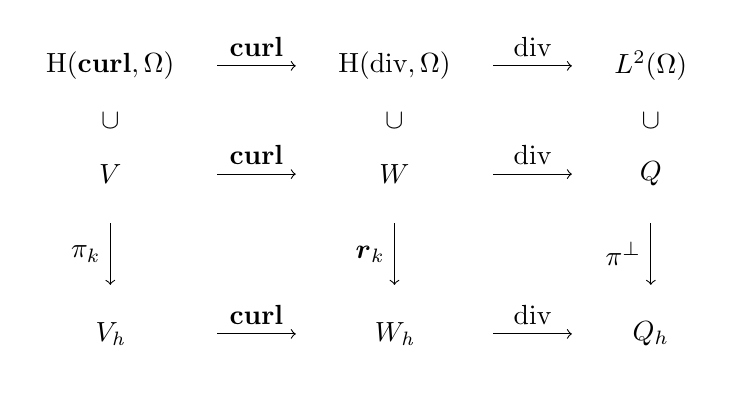
\begin{tikzpicture}[point/.style={circle, inner sep=0pt, minimum size=2pt,fill=red}]
            \matrix[column sep = 1.82mm, row sep = 1.1mm, ampersand replacement = \&] {
             \node {$\text{H}(\textbf{curl},\Omega)$};  
              \& \node (n0) {};
              \& \node      {};
              \& \node (n1) {};
              \& \node (n2) {};
              \& \node {$\text{H}(\Div, \Omega)$}; 
              \& \node (r1c7) {};
              \& \node {};
              \& \node {};
              \& \node (r1c10) {};
              \& \node {$L^2(\Omega)$};\\
             \node (n3) {}; \&\&\&\&\& \node (n5)   {};
              \& \node (r2c7) {};
              \& \node {};
              \& \node {};
              \& \node {};
              \& \node (r2c11) {};\\
             \node (n4) {}; \&\&\&\&\& \node (n6)   {};
              \& \node (r3c7) {};
              \& \node {};
              \& \node {};
              \& \node {};
              \& \node (r3c11) {};\\
             \node (v)  {$V$}; \&\node(fromV){};\&\&\&\node(toW){};\& \node (w) {$W$};
              \& \node (r4c7) {};
              \& \node {};
              \& \node {};
              \& \node (r4c10) {};
              \& \node {$Q$};\\
             \node (n7) {}; \&\&\&\&\& \node (n8)   {};
              \& \node {};
              \& \node {};
              \& \node {};
              \& \node {};
              \& \node (r5c11) {};\\
             \node      {}; \&\&\&\&\& \node        {}; 
              \& \node {};
              \& \node {};
              \& \node {};
              \& \node {};
              \& \node {};\\
             \node      {}; \&\&\&\&\& \node        {}; 
              \& \node {};
              \& \node {};
              \& \node {};
              \& \node {};
              \& \node {};\\
             \node (n11)    {}; \&\&\&\&\& \node (n12) {};
              \& \node {};
              \& \node {};
              \& \node {};
              \& \node {};
              \& \node (r8c11) {};\\
             \node {$V_{\textit{h}} $};                                 
              \& \node (n13) {};
              \& \node       {};
              \& \node (n14) {};
              \& \node (n15) {};
              \& \node {$W_{\textit{h}} $}; 
              \& \node (r9c7) {};
              \& \node {};
              \& \node {};
              \& \node (r9c10) {};
              \& \node {$Q_h$};\\
             };
            \draw[->] (n0) to node[above] {$\textbf{curl}$} (n2); 
            \draw[->] (fromV) to node[above] {$\textbf{curl}$} (toW); 
            \draw[white] (n3) to node {{\color{black}$\cup$}} (n4);
            \draw[white] (n5) to node {{\color{black}$\cup$}} (n6);
            \draw[->] (n7) to node[left] {$\pi_k$} (n11); 
            \draw[->] (n8) to node[left] {$\boldsymbol{r}_k$} (n12); 
            \draw[->] (n13) to node[above] {$\textbf{curl}$} (n15); 
            \draw[->] (r1c7) to node[above] {$\text{div}$} (r1c10);
            \draw[->] (r4c7) to node[above] {$\text{div}$} (r4c10);
            \draw[->] (r9c7) to node[above] {$\text{div}$} (r9c10);
            %\draw[white] (r2c7) to node {{\color{black}$\cup$}} (r3c7);
            \draw[white] (r2c11) to node {{\color{black}$\cup$}} (r3c11);
            \draw[->] (r5c11) to node[left] {$\pi^{\perp}$} (r8c11);
        \end{tikzpicture}
    \end{center}

% subsection definition_of_the_h_div_element (end)

El sigte lema, hacerlo una vez para edge
y una vez para face, para un cierto poliedro, y decir que vale 
la misma cuenta en los otros. Ver (3.79) (3.80) en monk: transf.
de normales y tangentes.\\\\
remite a transform entre prismas etc ... de preliminares
\begin{lemma} The edge element interpolators satisfy
\begin{IEEEeqnarray}{rCl}\label{piTransformado}
    \wku(\hat{\bx}) & = & M^{t} \bw_k\bu(F(\hat{\bx})).
\end{IEEEeqnarray}
{\color{BrickRed} > lo probamos?}
\end{lemma}

% subsection transformaciones_entre_prismas (end)
\begin{chapter}[Virtual Elements]{Virtual Elements}

The vems are customarly defined in terms of a given problem.

It is our intention to propose a Virtual Elements Method (VEM) scheme
as a generalization of $H(\text{div})$--conforming Finite Elements
in meshes consisting of polyhedra of arbitrary kind.
We deal with tetrahedra, triangular prisms and pyramids and, in the presence of
the latter, our VEM scheme is put in the framework of non-polynomial Finite Elements.\\[5pt]
\section{primera}
Recall Problem~\ref{weakMixedContinuous} and add some notation on
bilinear forms.
Let be given an open \emph{non--convex} domain $\Omega\subseteq\mathbb{R}^3$ with
Lipschitz--continuous boundary
consisting of planar faces and define $V:=H(\mbox{div},\Omega)$ and $Q:=L^2(\Omega)$.
Let us consider the following continuous problem.\\[5pt]
With 
\begin{IEEEeqnarray*}{rClCrCl}
	a(\bv,\bw) & = & \forma{v}{w} &\quad\mbox{and}\quad& b(\bv,q) & = & \formb{v}{q}
\end{IEEEeqnarray*}
find $\bu\in V$ and $p\in Q$ such that for every $\bv\in V$ and every $q\in Q$
\begin{equation}\label{mixedContinuousWeak}
  \makebox[0pt]{
    \begin{minipage}{\linewidth}
  	  \begin{IEEEeqnarray*}{rCCCl}
  		a(\bu,\bv) &+ &b(\bv,p) & = & 0\\[5pt]
  				   &- &b(\bu,q) & = & (f,q).
  	  \end{IEEEeqnarray*}
    \end{minipage}}
  \tag{MC}
\end{equation}
We start with a polihedral triangulation $\Th$ of $\Omega$ to define the 
virtual spaces $V_h$ and $Q_h$ as discretizations of $V$ and $Q$ respectively.\\[5pt]
For $E\in\Th$ the local space of vector fields will be
\begin{IEEEeqnarray*}{rCl}
  V_h(E)&=&\Big\{\bv\in H(\mbox{div},E)\cap H(\textbf{curl},E)\,:\,\\
  \yesnumber\label{vhE}
  &&\qquad \bv\cdot\bn|_f\in \mathcal P_0(f) \,\,\mbox{for all face $f$ of }E, \\
  && \qquad\dv\bv\in \mathcal P_0(E) \mbox{ and } \curl\bv = 0 \Big\}
\end{IEEEeqnarray*}
and the  global space $V_h$ will consist of functions defined piecewise with the former
local spaces:
\begin{IEEEeqnarray*}{ccrCl}
V_h&=&V_h(\Th)&:=&\Big\{\bv\in H(\dv,\Omega): \bv|_E\in V_h(E), \mbox{for all element }
E\in\Th\Big\}.
\end{IEEEeqnarray*}
\noindent{\color{blue}\#\#\#\#\#\#\# poner algo de por qu'e se pone
la condicion del curl: para que sea el gradiente de alguien (Nicaise)}. 
The scalar discrete space we will consider is
\begin{IEEEeqnarray}{rCl}
  Q_h & = & \mathcal{P}_0(\Th)
\end{IEEEeqnarray}
meaning the functions that are constant on each element of $\Th$. As expected,
with $V_h$ we consider the $H(\dv,\Omega)$ norm, 
$\|\bv\|^2_{V_h} = \|\bv\|^2_{L^2(\Omega)} + \|\dv\bv\|^2_{L^2(\Omega)}$,
and with $Q_h$ we consider the $L^2(\Omega)$ norm.

The condition in the definitions of these spaces suffice to construct an interpolation
operator, which is a key object both in Finite Elements as in Virtual Elements.
Let us take the degrees of freedom
\begin{IEEEeqnarray}{rCl}\label{dofs}
  \iint_f \bv\cdot\bn\,dS & \qquad\mbox{ for all face $f$ of } & \Th.
\end{IEEEeqnarray}
With \emph{faces of $\Th$} we mean the family of all faces forming the boundary
of the elements, with the unit normals consistently taken in the case of
neighbour elements.
\begin{lemma}\label{unisolvence} Given a polyhedron $E\in\Th$, the degrees
  of freedom~(\ref{dofs}) corresponding to the faces of $E$ are unisolvent
  in $V_h(E)$.
\end{lemma}
\begin{proof} \emph{Existence.} Let $n_{f,E}$ be the number of faces of $E$ and
take real numbers $\{\alpha_i\}_{i=1}^{n_{f,E}}$. Let $g$ the  piecewise constant
function on $\partial E$ satisfying, for all $i$, %face $f$ of $E$
\[
  \int\limits_{f_i} g = \alpha_i
\]
and let $d$ be the constant function in $E$ such that
\[
 \int\limits_E d\,d\textbf{x} = \sum \alpha_i.
\]
Then we consider the auxiliary problem of seeking a solution of
\begin{IEEEeqnarray}{rClrCl}
  \label{aux_prob}
  \Delta \phi & = & d \quad \mbox{in $E$,} \qquad & 
  \frac{\partial \phi}{\partial \bn}& = &g \quad \mbox{on }\partial E.
\end{IEEEeqnarray}
By definition we obtain the compatibility condition
\begin{IEEEeqnarray*}{rCl}
  \int\limits_E d\,d\textbf{x}& = & \int\limits_{\partial E} g\,d\gamma    
\end{IEEEeqnarray*}
so the solution $\phi$ to the problem~(\ref{aux_prob}) exists. Now
we take $\bu:=\nabla \phi$ and  it holds immediately that $\dv\bu$ is constant in $E$,
$\bu\cdot\bn$ is constant on each face of $\partial E$ and $\curl\bu = 0$. So
$\bu$ lies in $V_h(E)$ and also for all $1\leqslant i\leqslant n_{f,E}$ $\int_{f_i} \bu\cdot\bn\,d\gamma = \alpha_i$.\\[4pt]
\emph{Uniqueness.} Suppose that $\bv\in V_h(E)$ has vanishing
degrees of freedom. Condition $\curl\bv=0$ implies
$\bv=\nabla\phi$ for certain $\phi$. Now, since $\dv\bv$ is constant on $E$, the
relation
\begin{IEEEeqnarray*}{rCl}
   0 & = & \int\limits_{\partial P}\bv\cdot\bn\,d\gamma 
\end{IEEEeqnarray*} %& = & \int\limits_P\dv\bv\,d\textbf{x}
imply $\dv\bv=0$ by Green Theorem. Then, the potential $\phi$ satisfies
\begin{IEEEeqnarray*}{rClrCl}
  \Delta \phi & = & 0 \quad \mbox{in $E$,} \qquad & 
  \frac{\partial \phi}{\partial \bn}& = &0 \quad \mbox{on }\partial E
\end{IEEEeqnarray*}
which means it is a constant, and it follows $\bv=0$.
\end{proof}
With this Lemma already demonstrated we are able to consider
an $H(\text{div})$--like local interpolation operator well defined.
\begin{corollary} \label{interpolant}
  For every $\bv\in H^1(E)^3$ there exists a $V_h(E)$--interpolant $I(\bv)$
  defined as the unique element in $V_h(E)$ such that for every face $f$ of $E$
    \begin{IEEEeqnarray*}{rCl}
      \int\limits_f I(\bv)\cdot\bn\,d\gamma & = & \int\limits_f \bv\cdot\bn\,d\gamma.       
    \end{IEEEeqnarray*}
\end{corollary}
\begin{lemma} \label{p0_projection} Consider the projection $P_0$ onto the constants on $E$. It holds
\begin{IEEEeqnarray*}{rCl}
  \dv I(\bv) & = & P_0\,\dv\bv.
\end{IEEEeqnarray*}
\end{lemma}
\begin{proposition}\label{vem_equal_fem}
Recall the space $D_k$ introduced in~(\ref{dk}).\\
If $E$ is a right prism, then
\begin{IEEEeqnarray}{rCl}\label{d1p1}
  V_{\textit{h}}(E) & = & D_1(x,y)\otimes P_1(z)\mbox{,}
\end{IEEEeqnarray}
with $x,y,z$ being the variables in a cartesian system of coordinates in which
the $z$--axis is orthogonal to the planes containing the triangular faces of $E$.\\
If $E$ is a tetrahedron, then
\begin{IEEEeqnarray}{rCl}\label{p03}
  V_{\textit{h}}(E) & = & P_0^3(\bx) + P_0\bx\mbox{,}
\end{IEEEeqnarray}
with $\bx = (x,y,z)$ being the vector of variables in a cartesian system of coordinates.
\end{proposition}
\begin{proof}
  In the case of a prism $E$, the space $D_1(x,y)\otimes P_1(z)$ can be written as
  \[
    \{\bv \in P_1(E)\,:\, \bv=(a+\gamma x,b+\gamma y,c+d z),
        a,b,c,d,\gamma\in\mathbb{R})\}
  \]
  and then it is inmediately seen that it has the same dimension five
  as $V_{\textit{h}}(E)$. Finally, recalling that the $\dv$ and $\curl$ operators
  can be computed in the chosen local variables, given $\bv\in D_1(x,y)\otimes P_1(z)$
  we can compute $\bv|_{f}\cdot\bn_f$ on each face of $E$, $\dv\bv$ and $\curl\bv$
  to verify explicitly that the space on the right side of~(\ref{d1p1}) fulfills the 
  definition of $V_h(E)$ given in~(\ref{vhE}).
  Exactlty the same argument works for the case of a tetrahedron $E$, in which we
  deal with two vectorial spaces of dimension four that are such that 
  every element in
  \[
    P_0^3(\bx) + P_0\bx=\{\bv \in P_1(E)\,:\,
    \bv=(a+\gamma x,b+\gamma y,c+\gamma z,
    a,b,c,\gamma\in\mathbb{R})\}
  \]
  fulfills the conditions defining $V_{\textit{h}}(E)$.
\end{proof}
\begin{remark}
  By Proposition~\ref{vem_equal_fem} the spaces $V_h(E)$ conicide with the
  lowest order $H(\dv)$--conforming local Finite Element spaces
  introduced in~(\ref{prismaticSpace})
  for the prismatic case and in~(\ref{tetrahedralSpace}) for the tetrahedral case.
\end{remark}
\begin{lemma}
  The definition of the lowest order $H(\dv)$ Finite Elements on
  right prisms or tetrahedra is independent of
the choice of the cartesian axes (as long as the $z$-axis is
perpendicular to the trianguar faces in case of prisms).
\end{lemma}
\begin{proof}
  This can be prooved by hand. Let us proove the case of a Prism $E$. Let $(x,y,z)$ and $(x',y',z')$ be two cartesian coordinate systems satisfying the required properties. Then we can write
  \begin{IEEEeqnarray*}{rCl}
    x & = & p+\alpha x'-\beta  y' \\
    y & = & q+\beta x' -\alpha y' \\
    z & = & r+z'
  \end{IEEEeqnarray*}
for $\alpha$ and $\beta$ satisfying $\alpha^2+\beta^2 = 1$.
Let 
$\bv$ be an element in $V_{\textit{h}}(E)$. So
\begin{IEEEeqnarray*}{rCl}
\bv(x,y,z) & = & (a+\gamma x,b+\gamma y,c+d z)^{\scriptstyle t}\\
&=&\left((a+\gamma p) + \gamma(\alpha x' - \beta y'),
         (b+\gamma q) + \gamma(\beta x'+\alpha y'),
         (c+dr)+dz'\right)^{\scriptstyle t}.
\end{IEEEeqnarray*}
Then, the components of $\bv$ in the new coordinate versors are
\begin{IEEEeqnarray*}{rCcCl}
  \bv\cdot(\alpha,\beta,0)^{\scriptstyle t} & = &
   (\alpha a + \beta b + \gamma(\alpha p + \beta q )) +\gamma x' & =: & a' + \gamma x' \\
  \bv\cdot(-\beta,\alpha,0)^{\scriptstyle t} & = &
   (-\beta a + \alpha b + \gamma(-\beta p + \alpha q )) +\gamma y' & =: & b' + \gamma y' \\
  \bv\cdot(0,0,1)^{\scriptstyle t} & = &
   (c+dr)+d z' & =: & c' + dz'.
\end{IEEEeqnarray*}
Is follows that, in the $x'y'z'$ system,
\[
  \bv(x',y',z') = (a' + \gamma x', b' + \gamma y', c' + dz')^{\scriptstyle t}
  \in D_1(x',y')\otimes P_1(z').
\]
\end{proof}
%\paragraph{discretized forms} % (fold)
%\label{par:discretized_forms}
%\[
%\noindent{\color{blue}\#\#\#\#\#\#\# \mbox{¿hace falta?}} 
%  a(\bv,\bw)=\sum_{E\in\mathcal T_h}a^E(\bv,\bw), \qquad
%  b(\bv,q)=\sum_{E\in\mathcal T_h}b^E(\bv,q).
%\]
Next, together with the finite dimensional spaces already defined,
discretized version of the bilinear forms.\\
The evaluation of the form $b(\cdot,\cdot)$ in $(\bv,q)\in V_h\times Q_h$ can
be computed using the degrees of freedom~(\ref{dofs}) applied to $\bv$. For if $q\in Q_h$, then
\[
  b(\bv,q)=\int_\Omega q\,\dv\bv = \sum_{E\in\mathcal T_h}
  \int_Eq\,\dv\bv = \sum_{E\in\mathcal T_h}\int_{\partial E}q \bv\cdot\bn.
\]
so in the case of the form $b_h(\bv,q)$ we put simply
\[
  b_h(\bv,q) = b(\bv,q) =
  \sum_{E\in\mathcal T_h}b^E(\bv,q)\mbox{,}
\]
where $b^E(\bv,q) = \int_Eq\,\dv\bv\,d\textbf{x}$.
For the bilinear form $a(,)$, we can decompose it as
\[
  a(\bv,\bw)=\sum_{E\in\mathcal T_h}\int_E\bv\cdot\bw\,d\bx
\]
but this is not computable from the 
degres of freedom. The following construction
is done in order to get a calculable discrete form and
also we will introduce a term for the
stability.\\[4pt]
For each element $E\in\mathcal{T}_{\textit{h}}$, let the space $W(E)$
be defined by
\begin{IEEEeqnarray*}{rCl}
  W(E) & = & \left\{ \bw\in V_h(E):  \bw = \nabla  q_2,
\mbox{ for some }  q_2\in P_2(E)\right\}\\[5pt]
       & = & V_h(E)\cap\nabla {P}_2(E)\mbox{,}
\end{IEEEeqnarray*}
and with these we consider $W(\mathcal{T}_{\textit{h}}) = \{{\bw} : {\bw}|_{E} \in W(E)
\mbox{ for each }E\in\mathcal{\textit{h}}\}$. Integrating arbitrary elements
in~(\ref{d1p1}) and~(\ref{p03}) yields the following result.
\begin{lemma} When $E\in\mathcal{T}_{\textit{h}}$ is a tetrahedron or 
a prism, then $W(E) = V_{\textit{h}}(E)$.  
\end{lemma}
Again, observe that if $\bv\in V_h(E)$ and $\hat\bu\in\hat V(E)$, $a^E(\hat\bu,\bv)$ can be 
computed using the degrees of freedom of $\bv$, because it holds
\begin{IEEEeqnarray*}{rCCCl}
a^E(\hat\bu,\bv) &:=& \int_E\hat\bu\cdot\bv &=& \int_E\nabla \hat q_2\cdot\bv\\
                 &=&-\int_E\hat q_2 \dv\bv &+& \int_{\partial E}\hat q_2\bv\cdot\bn.
\end{IEEEeqnarray*}
This means we can consider an auxiliary projection  operator $\pi^E$
from $H(\dv,E)$ onto $W(E)$ defined by
\begin{IEEEeqnarray}{rCl}\label{projection}
  a^E(\bv-\pi^E\bv,\bw) = 0 &\qquad& \mbox{for all }\bw\in W(E)
\end{IEEEeqnarray}
fully computable in terms of the degrees of freedom of $\bv$.

We need the following last object to complete the discretization of $a(\cdot,\cdot)$.
Thanks to Lemma~\ref{unisolvence} we can consider a basis $B=\{\bv_{i,E}\}$
of $V_h(E)$ dual to the functionals~(\ref{dofs}), that is, for every
$1\leqslant i,j\leqslant n_{f,E}$
\begin{IEEEeqnarray}{rCl}
  \iint_{f_j} \bv_{i,E}\cdot\bn_j\,dS & = & \delta_{i,j}.
\end{IEEEeqnarray}
What we are considering is the inner product
$\mathcal \langle(\bv)_B,(\bw)_B\rangle$ of the coordinates
of the fields $\bv,\bw\in V_h(E)$ with respect 
to this local dual basis $B$.

Finally, the local discrete form $a_h^E$ is stated in the following definition.
\begin{defi} Given an element $E\in\Th$, for $\bv$ and $\bw$ in $V_{\textit{h}}(E)$
\begin{IEEEeqnarray}{rCl}\label{discreteLocal_a}
  a^E_{\textit{h}}(\bv,\bw) &:=& a^E(\pi^E\bv,\pi^E\bw) + 
  h_E^{-1}\langle(\bv-\pi^E\bv)_B,(\bw-\pi^E\bw)_B\rangle
\end{IEEEeqnarray}  
where $h_E$ is the diameter of $E$.
\end{defi}
The discrete global form $a_h$ is defined by the following equation.
\[
  a_h(\bv,\bw) = \sum_{E\in \mathcal T_h} a_h^E(\bv|_E,\bw|_E),
    \quad\mbox{ for } \bv \mbox{ and } \bw \in V_h.
\]

One fact to note
about the projection $\pi^E$ in~(\ref{projection}) is that, by
Remark~\ref{vem_equal_fem},
it coincides with the identity $I:W(E)\to W(E)$ whenever the element $E\in\Th$
is a Prism or a Tetrahedron so that, immediately, we have the following
property.
\begin{remark}\label{ah_equal_a} If $E$ is a tetrahedron or a prism, then
  $a_h^E(\bv,\bw)=a^E(\bv,\bw)$ for all $\bv,\bw \in V_h(E)$.
\end{remark}
Now we state a key result concerning the stability of the
discrete form $a^E_{\textit{h}}$ and which explains the form of the
term $h_E^{-1}\langle\,\cdot\,,\cdot\,\rangle$ in~(\ref{discreteLocal_a}).
\\{\color{blue}\#\#\#\#\#\#\#\# prop 3.2...}

In what follows we analyse the second term in $a_h^E$ when $E$ is a pyramid.
In this case, denote by $\{\bv_i\}$ the dual basis of the degrees of freedom \eqref{degreeOfFreedom}, that is,
\[
\bv_i\in V_h(E), \qquad \mbox{and}\qquad \int_{f_j}\bv_i\cdot\bn =\delta_{i,j}, \quad 1\le i,j\le 5,
\]
if $f_i$, $i=1,\ldots,5$, denote the faces of $E$. Then $\bv\in V_h(E)$ can be uniquely written as
\[
\bv=\sum_{i=1}^5 a_i \bv_i,
\]
with
\[
a_i=\int_{f_i}\bv\cdot\bn.
\]
By setting
\[
\vertiii{\bv}_E^2=\frac1{h_E}\sum_{i=1}^5 a_i^2
\]
$\vertiii{\cdot}_E$ defines a norm on $V_h(E)$, and since it has a finite dimension, we know that for constants $c_E$ and $C_E$, which depend on $E$, we have
\begin{equation}\label{equiv0}
c_E\|\bv\|_{L^2(E)}\le \vertiii{\bv}_E\le C_E\|\bv\|_{L^2(E)}, \qquad \forall \bv\in V_h(E).
\end{equation}
The purpose of the next Proposition is to prove that $C_E$ and $c_E$ can be taken depending only on the aspect ratio of $E$.


% \textcolor{red}{
% {\bf Assumption (A).} We assume that if $\mbox{diam\,}E=1$, constants $c$ and $C$ above depends only on the shape-regularity of $E$.
% }

\begin{proposition}
\label{stabilizing_term}
Let $E$ be a pyramid, and consider the basis $\{\bv_i, i=1,\ldots,5\}$ of $V_h(E)$, and the associated discrete norm $\vertiii{\cdot}_E$ introduced above. Then there exist constants $C_E$ and $c_E$ depending only on the aspect ratio of $E$ such that \eqref{equiv0} holds true for all $\bv\in V_h$.
\end{proposition}
\begin{proof} First we note that if $\bv\in V_h(E)$ is given by
\[
\bv = \sum_{i=1}^5a_i\bv_i
\]
then it satisfies
\[
\bv = \nabla\phi
\]
with 
\begin{eqnarray}\label{a0}
\Delta\phi &=& d\qquad \mbox{in }E\\ \frac{\partial\phi}{\partial\bn}&=& g\qquad\mbox{on }\partial E\nonumber\\ \int_E\phi&=&0\nonumber
\end{eqnarray}
for
\begin{equation}\label{ai}
g|_{f_i}=\frac{a_i}{|f_i|},\quad 1\le i\le5, \qquad |E|d=\sum_{i=1}^5a_i.
\end{equation}
Given $q\in H^1(E)$, we multiply  the first equation of \eqref{a0} by $q$ and integrate on $E$, integrate by parts on the left hand side, and use the Neumann boundary conditions to have
\[
\int_E\nabla\phi\cdot\nabla q = -\int_Edq + \int_{\partial E}gq.
\]
Since 
\[
\|\bv\|_{L^2(E)}=\|\nabla\phi\|_{L^2(E)}=\sup\left\{\int_{E}\nabla\phi\cdot\nabla q: \,\, q\in H^1(E),\|\nabla q\|_{L^2(E)}=1,\int_Eq=0\right\}
\]
we conclude that
\begin{equation}\label{equi0}
\|\bv\|_{L^2(E)}=\sup\left\{-\int_Edq + \int_{\partial E}gq: \,\, q\in H^1(E),\|\nabla q\|_{L^2(E)}=1,\int_Eq=0\right\}.
\end{equation}
Since $d$ and $g$ can be written in terms of $a_i$, we have obtained an expression of the norm $\|\bv\|_{L^2(E)}$ in terms of the coefficients of $\bv$ in the basis.
Now, let $\hat E$ be a reference pyramid, and $F:\hat E\to E$ a affine transformation mapping $\hat E$ onto $E$ (remember that only pyramids with parallelogram basis are considered), which can be written as
\[
{\bf x}=F(\hat{\bf x})=B\hat{\bf x}+{\bf c}.
\] 
Given $q\in H^1(E)$ we define $\hat q$ by
\[
\hat q(\hat{\bf x}) = q({\bf x}),\qquad \forall \hat{\bf x}\in \hat E
\] 
and we observe that there exists constants $c_0$ and $c_1$ depending on the aspect ratio of $E$ such that
\begin{equation}\label{a1}
\frac{c_0}{h_E}\|\nabla q\|_{L^2(E)}^2\le \|\nabla\hat q\|_{L^2(\hat E)}^2\le \frac{c_1}{h_E}\|\nabla q\|_{L^2(E)}^2,
\end{equation}
and, on the other hand,
\[
\int_{\hat E}\hat q =0\quad \Longleftrightarrow \quad\int_Eq=0.
\]
We have
\[
-\int_Edq + \int_{\partial E}gq = \|\nabla \hat q\|_{L^2(\hat E)}\left(-\int_{\hat E}d\frac{\hat q}{\|\nabla\hat q\|_{L^2(\hat E)}}|B| + \int_{\partial \hat E}\hat g\frac{\hat q}{\|\nabla\hat q\|_{L^2(\hat E)}} |J|\right)
\]
with $\left|J(\hat{\bf x})\right|_{f_i}|= |f_i|/|\hat f_i|\sim h_E^2$. It follows that
\begin{multline*}
\|\bv\|_{L^2(E)}=\sup\Bigg\{\|\nabla \hat q\|_{L^2(\hat E)}\left(-\int_{\hat E}d|B|\frac{\hat q}{\|\nabla\hat q\|_{L^2(\hat E)}} + \int_{\partial \hat E}g|J|\frac{\hat q}{\|\nabla\hat q\|_{L^2(\hat E)}} \right):\\ \quad q\in H^1(E),\|\nabla q\|_{L^2(E)}=1,\int_Eq=0\quad\Bigg\},
\end{multline*}
and taking \eqref{a1} into account we obtain
% \begin{multline*}
% \|\bv\|_{L^2(E)}\le \sup\Bigg\{\|\hat \nabla q\|_{L^2(\hat E)}\left(-\int_{\hat E}d|B|\frac{\hat q}{\|\nabla\hat q\|_{L^2(\hat E)}} + \int_{\partial \hat E}g|J|\frac{\hat q}{\|\nabla \hat q\|_{L^2(\hat E)}} \right):\\ \quad \hat q\in H^1(\hat E),\frac{c_0}{h_E^\frac12}\le\|\nabla \hat q\|_{L^2(\hat E)}\le\frac{c_1}{h_E^\frac12},\int_{\hat E}\hat q=0\quad\Bigg\}
% \end{multline*}
\begin{equation}\label{mult1}
\|\bv\|_{L^2(E)}\le  \frac{c_1^\frac12}{h_E^\frac12}\sup\Bigg\{\left(-\int_{\hat E}d|B|\hat q + \int_{\partial \hat E}g|J|\hat q \right): \quad \hat q\in H^1(\hat E),\|\nabla \hat q\|_{L^2(\hat E)}=1,\int_{\hat E}\hat q=0\quad\Bigg\}
\end{equation}
and 
\begin{equation}\label{mult2}
\|\bv\|_{L^2(E)}\ge  \frac{c_0^\frac12}{h_E^\frac12}\sup\Bigg\{\left(-\int_{\hat E}d|B|\hat q + \int_{\partial \hat E}g|J|\hat q \right): \quad \hat q\in H^1(\hat E),\|\nabla \hat q\|_{L^2(\hat E)}=1,\int_{\hat E}\hat q=0\quad\Bigg\}.
\end{equation}
% and so
% \begin{multline*}
% \|\bv\|_{L^2(E)}\le \frac{c_1}{h_E^\frac12}\sup\Bigg\{-\int_{\hat E}d|B|\hat q + \int_{\partial \hat E}g|J|\hat q:\\ \quad \hat q\in H^1(\hat E),\|\nabla \hat q\|_{L^2(\hat E)}=1,\int_{\hat E}\hat q=0\quad\Bigg\}.
% \end{multline*}
We remark that
\[
\int_{\hat E}d|B|=\int_{\partial\hat E}g|J|,
\]
Now, let $\{\hat\bv_i\}$ be the dual basis of $V_h(\hat E)$ to the degrees of freedom, and let
\begin{equation}\label{hatai}
\hat a_i=g|_{f_i}|J|_{f_i}|\hat f_i|, \qquad i=1,\ldots,5.
\end{equation}
and
\[
\hat\bv = \sum_{i=1}^5 \hat a_i\hat\bv_i.
\]
Then, from \eqref{equiv0} for $\hat E$ we know that
\begin{equation}\label{equiv1}
c_{\hat E}^2\|\hat\bv\|_{L^2(\hat E)}^2\le \frac1{h_{\hat E}}\sum_{i=1}^5 \hat a_i^2\le C_{\hat E}^2\|\hat\bv\|_{L^2(\hat E)}^2 
\end{equation}
and using \eqref{equi0} for $\hat E$ instead of $E$ we have %(with constants in the equivalence depending only on $\hat E$) %from our previous reasoning %(with $h_{\hat E}\sim 1$)
\[
\|\hat\bv\|_{L^2(\hat E)}= \sup\Bigg\{\left(-\int_{\hat E}d|B|\hat q + \int_{\partial \hat E}g|J|\hat q \right): \hat q\in H^1(\hat E),\|\nabla \hat q\|_{L^2(\hat E)}=1,\int_{\hat E}\hat q=0\Bigg\}.
\]
It follows from \eqref{equiv1} that
\[
\left(\frac1{h_{\hat E}}\sum_{i=1}^5 \hat a_i^2\right)^\frac12\sim \sup\Bigg\{\left(-\int_{\hat E}d|B|\hat q + \int_{\partial \hat E}g|J|\hat q \right): \hat q\in H^1(\hat E),\|\nabla \hat q\|_{L^2(\hat E)}=1,\int_{\hat E}\hat q=0\Bigg\},
\]
where the constants in this equivalence depend on the aspect ratio of $E$, and so, since $h_{\hat E}\sim 1$, this equation together with \eqref{mult1} and \eqref{mult2} gives
\[
\frac1{h_E}\sum_{i=1}^5\hat a_i^2\sim \|\bv\|_{L^2(E)}^2.
\]
But, from \eqref{ai} and \eqref{hatai}
\[
\hat a_i = a_i\frac{|J|_{f_i}|}{|f_i|}|\hat f_i|\sim a_i, \qquad i=1,\ldots,5,
\]
and then we obtain
\[
\frac1{h_E}\sum_{i=1}^5a_i^2\sim \|\bv\|_{L^2(E)}^2
\]
as we wanted, since the constants in this equivalence depend only on the aspect ratio of $E$.
\end{proof}

As a consequence of this result we obtain the next Corollary.

Proposition~(\ref{stabilizing_term}) yields the next corollary.
\begin{corollary}\label{equivalence} For all $\bv\in V_h(E)$ and all pyramidal
$E\in\mathcal T_h$ it holds
\begin{IEEEeqnarray*}{rCcCl}
  c_E\,a^E(\bv,\bv) & \leqslant & h_E^{-1}\langle(\bv)_B,(\bv)_B\rangle & \leqslant
  & C_E\,a^E(\bv,\bv)
\end{IEEEeqnarray*}
where $c_E$ and $C_E$ depend only on the shape regularity of $E$.
\end{corollary}

\section{discrete problem.}
The discrete problem in the Finite--Virtual Element scheme is stated as follows.
\begin{problem}\label{mixedDiscrete}
To find $\bu_{\Th}\in V_{\Th}$ and $p_{\Th}\in Q_{\Th}$ such that
$\forall \bv\in V_{\Th} \forall q\in Q_{\Th} $
\begin{equation}
  \makebox[0pt]{
    \begin{minipage}{\linewidth}
      \begin{IEEEeqnarray*}{rCCCl}
        a_{\scriptscriptstyle\Th}(\bu_{\Th},\bv) & + & b(\bv,p_{\Th}) & = & 0 \\[5pt]
                               & - & b(\bu_{\Th},q) & = & (f,q)
      \end{IEEEeqnarray*}
    \end{minipage}}
  %\tag{MD}
\end{equation}
\end{problem}
In Section~\ref{sec:well_posedness} we will be concerned in proving existence
and uniqueness for Problem~(\ref{mixedDiscrete}). It will be done
showing coercivity for one of the bilinear forms and a
discrete version of the $\inf$--$\sup$ condition for the other.
\begin{lemma}\label{lemma_for_coercivity} For all $E\in\Th$, all $\bu\in W(E)$ and all $\bv\in V_h(E)$
\begin{IEEEeqnarray}{rCcCl} 
a_h^E(\bu,\bv) & = & a^E(\bu,\bv)       & &\label{L1}\\
c_E\,a^E(\bv,\bv)      & \leqslant & a_h^E(\bv,\bv) & \leqslant & C_E\,a^E(\bv,\bv)\label{L2}
\end{IEEEeqnarray}
with $c_E = C_E = 1$ when $E$ is tetrahedral or prismatic and $c_E,C_E$ depending
only on the shape regularity of $E$ when $E$ is pyramidal.
\end{lemma}
\begin{proof} The relation $\hat\bu=\hat\pi^E\bu$, condition~(\ref{projection})
and the symmetry of $a^E$ imply
\[
  a_h^E(\hat\bu,\bv)=a^E(\hat\pi^E\hat\bu,\hat\pi^E\bv)=a^E(\hat\pi^E\hat\bu,\bv)=a^E(\hat\bu,\bv)
\]
which proves~(\ref{L1}).
To prove~(\ref{L2}), if $E$ is not a Pyramid this property is already a consequence
of~(\ref{ah_equal_a}). In the case of a Pyramid, firstly a simple computation yields
\begin{IEEEeqnarray}{rCcCl}
  \label{comput}
  a^E(\bv,\bv)&=&a^E(\bv-\hat\pi^E\bv,\bv-\hat\pi^E\bv)&+&a^E(\hat\pi^E\bv,\hat\pi^E\bv).
\end{IEEEeqnarray}
Corollary~\ref{equivalence} and~(\ref{comput}) give
\begin{IEEEeqnarray*}{rCl}
a_h^E(\bv,\bv) &\leqslant& a^E(\hat\pi\bv,\hat\pi\bv) + C_E\,a^E(\bv-\hat\pi\bv,\bv-\hat\pi\bv) \\[5pt]
               &\leqslant& \max\{1,C_E\}\,a^E(\bv,\bv).
\end{IEEEeqnarray*}
In a similar manner, it holds
\[
  a_h^E(\bv,\bv)\geqslant \min{1,c_E}\,a^E(\bv,\bv).
\]
\end{proof}



\section{A Projection Space $W(E)$}
Since it holds clearly that $W(E)=V_h(E)$ when $E$ is a tetrahedron or a prism,
the purpose of this Section is to characterize $W(E)$ only when $E$ is a pyramid.
The Section finishes with some computational insights. 
\begin{lemma}\label{L3}
Let $\hat E$ be the reference pyramid 
of Definition~\ref{defi_of_ref_pyr} and recall the notation for the faces
in Table~\ref{pyramidNotationTableFaces}.
If $\hat\bv\in P_1(\hat E)^3$ verifies $\hat\bv \cdot \hat\bn =0$ on
$\hat f_1$, $\hat f_2$, $\hat f_3$ and
$\hat f_5$, then $\hat\bv(\hat\bx)=(0,c\hat x_2,0)$ for a constant $c$.
\end{lemma}
\begin{proof}
The conditions of $\hat\bv\cdot\hat\bn$ over the faces $\hat f_1$, $\hat f_2$ and
$\hat f_5$ yield
\[
\hat\bv(\hat\bx) = (b_1\hat x_1, c_2\hat x_2,d_3\hat x_3)'.
\]
Using that $\hat\bv\cdot\hat\bn=0$ on
$\hat f_3$  we have $b_1=d_3=0$. Then $\hat \bv=(0,c_2\hat x_2,0)'$ as we wanted to prove.
\end{proof}
\begin{lemma}\label{L4}
Let $P$ be any pyramid on a physical mesh. Then $\mbox{dim\,}W(P)\leqslant 4$.
\end{lemma}
\begin{proof}
As $W(P)\subseteq V_{\textit{h}}(P)$, we have $\mbox{dim\,}W(P)\leqslant 5$. 
We will prove that $W(P)\ne V_{\textit{h}}(P)$ by showing that there exists no field
$\bv=\nabla q_2$ for $q_2\in P_2(P)$ if we impose the restriccion that the normal
component of $\bv$ vanishes on four different faces of $P$ while is different from zero on
the remaining face.

Let $\hat E$ be the reference pyramid of Definition~\ref{defi_of_ref_pyr}  and
let us use the same notation for the faces. Let $F(\hat {\bx}) = M_P \hat{\bx} + \bx_P$
be an affine map from $\hat E$ onto $P$ and let
$f_i=F(\hat f_i)$ denote the faces of $\hat E$ and $P$. Suppose
that $\bv=\nabla q_2$ for a $q_2 \in P_2(P)$ and that
$\bv\cdot\bn=0$ on $f_1$, $f_2$, $f_3$ and $f_5$, while
$\bv\cdot\bn=1$ on $f_4$. Now we transform it with~(\ref{transfDiv}) to get
\begin{equation}\label{piola}
\bv({\bx}) = \frac1{|M_P|}M_P\hat\bv(\hat{\bx}), \qquad {\bx}=F(\hat {\bx}),
\end{equation}
where $\hat\bv$ is in $P_1(\hat E)^3$. If $\phi\in P_1(f_i)$, put $\hat\phi = \phi\circ F$.
Using the properties of the transformed
degrees of freedom we explained in Section~\ref{auxlabel110} we have, for $i=1,2,3,5$,
\[
\iint_{\hat f_i}\hat\bv\cdot {\hat\bn}\,\hat\phi\,d\hat S = \iint_{f_i}\bv\cdot {\bn}\,\phi\,dS =0
\]
for all $\phi\in P_1(f_i)$.
Since $\hat\bv|_{\hat f_i}\cdot {\hat\bn}$ is itself a $P_1(\hat f_i)$ polynomial, 
this implies $\hat\bv|_{\hat f_i}\cdot {\hat\bn}$ vanishes identically over $\hat f_i$.
By Lemma~\ref{L3} we have $\hat\bv(\hat{\bx})=(0,c\hat x_2,0)'$. Then
\[
  \bv({\bx})=\frac1{|M_P|}M_P(0,c\hat x_2,0)' = \frac {c\,\hat x_2}{|M_P|}\boldsymbol{m}_2 
\]
where we write $M_P=[\boldsymbol{m}_1\,\,\boldsymbol{m}_2\,\,\boldsymbol{m}_3]$ 
columnwise. So on $f_4$ we have 
\[
	\bv({\bx})\cdot {\bn}=\frac {c\,\hat x_2}{|M_P|}\boldsymbol{m}_2\cdot {\bn} 
\]
but $\hat x_2$ is not a constant on $f_4$ since it ranges from $0$ to $1$. Moreover,
$\boldsymbol{m}_2\cdot {\bn}$ is not zero because $\boldsymbol{m}_2$ is a 
vector {\color{Orange}\#\#\#\#\#\#\#\# quiere decir no perpend? transversal} to $f_4$.
Then $\bv({\bx})\cdot {\bn}$ is not a constant on $f_4$, which contradicts our 
definition of $\bv$.  
\end{proof}
Now we explicit the pyramidal projection space.
\begin{proposition}
Let $P$ be a pyramid in the mesh. Then $W(P)=P_0^3(P)+{\bx} P_0(P)$.
\end{proposition}
\begin{proof}
First $P_0^3(P)+{\bx} P_0(P)\subseteq W(P).$
Since by Lemma~\ref{L4} both spaces have the same dimension the assertion concludes.
\end{proof}
If $P$ is a physical pyramid, given a field $\bv \in V_h(P)$ we can construct $\pi^P\bv$
as follows. We choose a basis $\{\bw_i\}$ of $W(P)$, for
example,
\[
\left\{ (1,0,0)', (0,1,0)', (0,0,1)', (x,y,z)' \right\} =: \{
\bw_i: 1\leqslant i\leqslant 4\}
\]
with $\bw_i=\nabla q_i$, $i=1,2,3,4$. Then $a^P(\bv,\bw_i)$ is 
calculable from the degrees of freedom of $\bv$ by
\[
a^P(\bv,\bw_i) = \int_P\bv\cdot\nabla q_i\,d\bx =
-\int_P\mbox{div\,}\bv\,q_i\,d\bx + \iint_{\partial P}\bv\cdot\bn\,q_i\,dS.
\]
Then, if $\pi^P\bv=\sum_{j=1}^4\alpha_j\bw_j$ we can
compute the coefficients $\alpha_j$ by solving the linear system
\[
\sum_{j=1}^4\alpha_j a^P(\bw_j,\bw_i) =
a^P(\bv,\bw_i), \qquad 1\leqslant i\leqslant 4.
\]
In order to compute the stabilization part of the discrete
bilinear form $a_\textit{h}^P$ we need to write $\pi^P\bv$ in terms
of the basis $\{\bv_i\}$ of $V_h(E)$ associated with
the degrees of freedom. That is (always in the pyramidal case)
\[
\iint_{f_i}\bv_j\cdot\bn\,dS =\delta_{ij}, \qquad 1\leqslant i,j\leqslant 5.
\]
In this case, we have $\pi^P\bv = \sum_{i=1}^5\beta_i\bv_i$,
with
\[
\beta_i=\sum_{j=1}^4\alpha_j\iint_{f_i}\bw_j\cdot\bn\,dS.
\]
\end{chapter}

\chapter{Local Interpolation}
We prove anisotropic local interpolation error estimates for two different operators
and use this result to estimate the global approximation error.

Edge elements are one example of $\textrm{H}(\textbf{curl})-$conforming elements, and they were
defined to determine a natural interpolation operator for fields with continuous tangential components.
Similarly, the other elements considered are $\textrm{H}(\text{div})-$conforming, and we will use them 
to interpolate fields with continuous tangential components. These are the cases of the
solutions of Stokes' equations, the solutions of time harmonic Maxwell's equations, and the vectorial
variable of the following problem, which will be our application.
\section{Prismatic Finite Elements} % (fold)
\label{sec:prismatic_finite_elements}
\subsection{Stability of curl--conforming Finite Element on Prisms}
\label{stab_edge_prism}
\section{Stability of the Edge Element in $\hat{K}$}
In the next three Lemmas $\hat\bu$ is an element
in $H({\bf curl},\hat{E})$ and we will assume there are 
a positive $\delta$ and a $p>2$ such that 
$\hat\bu$ belongs to $H^{1/2+\delta}(\hat{E})^3$ and
${\bf curl}\,\bu$ belongs to $L^p(\hat{E})^3$.
\begin{lemma}\label{lema_PIu3_k_cualquiera} 
$(\wku)_3$ is linearly and univocally 
determined by $\hat{u}_3$.
\end{lemma}
\begin{proof} If we pay attention to the directions of the unit
tangents and normals to the edges and faces, respectively, of $\hat E$,
we realize that
the degrees of freedom which involve $\wku_3$ give rise onnlyto the 
following linear equations
\begin{IEEEeqnarray}{rCrc}
\varphi_{e_i,p}\,(\wku) & = & \varphi_{e_i,p}\,(\hat{\bu}) &\quad\mbox{for $i$ = 3, 6, 7 and }p\in\mathcal{}  \\
\varphi_{f_j,\boldsymbol{q}}\,(\wku) & = & \varphi_{f_j,\boldsymbol{q}}\,(\hat{\bu})
  &\quad\mbox{for $j$ = 1, 2, 4 and }\boldsymbol{q}\in\mathcal{}  \\
\varphi_{\boldsymbol{r}}\,(\wku) & = & \varphi_{\boldsymbol{r}}\,(\hat{\bu})
  &\quad\mbox{for }\boldsymbol{r}\in\mathcal{}.
\end{IEEEeqnarray}
These are 
$3k$+$3k(k-1)$+$k(k-1)(k-2)/2 = k(k+1)(k+2)/2$ equations,
just the dimension of $P_k(\hat{T})\otimes P_{k-1}(\hat{I})$, 
which is the space $(\wku)_3$ belongs to by definition.
%$\frac{k(k+1)(k+2)}{2}$. 
%libertad en los que no des\-a\-pa\-re\-ce $(\pi\textbf{u})_3$ son \'unicamente:
Now set all those equations to zero and see that the unique solution is $(\wku)_3 = 0$.
A little more explicitly, we have:
\noindent{\color{blue}\#\#\#\#\#\#\# } 
para cada arista $e_j$, $j = 3, 6, 7$,
\begin{IEEEeqnarray}{lClc}
  \label{aristas} \int\limits_{e_j} (\pi\textbf{u})_3 q \, ds 
  & = & 0 &\quad q\in P_{k-1}(e_j).
\end{IEEEeqnarray}
Para cada cara vertical $f=f_1$, $f_2$, $f_4$,
\begin{IEEEeqnarray}{lClc}
	\label{caras} \int\limits_{f} (\pi\textbf{u})_3 q \, 
	d\gamma & = & 0 &\quad q\in Q_{k-2,k-1}(f_{ijkl}).
\end{IEEEeqnarray}
En $\hat{K}$
\begin{IEEEeqnarray}{lClc}
	\label{enK} \int\limits_{\hat{K}} (\pi\textbf{u})_3 
	q \, d\textbf{x} & = & 0 &\quad q\in P_{k-3}(f_z) \otimes P_{k-1}(e_{xy}).
\end{IEEEeqnarray}
\noindent{\color{blue}\#\#\#\#\#\#\# }
 of freedom que estos grados de libertad se anulan todos y veamos que de esta suposici\'on
se deduce que $(\pi\textbf{u})_3 = 0$, es decir que las ecuaciones li\-nea\-les mencionadas determinan un\'ivocamente a un elemento
$(\pi\textbf{u})_3$ pertenenciente a 
$P_k(\hat{T}) \otimes P_{k-1}(\hat{I})$. 

Empezamos por ver que $(\pi\textbf{u})_3$ se anula en ciertos subconjuntos de 
$\partial \hat{K} $. La restricci\'on de $(\pi\textbf{u})_3$ a $e_j, (j=3,6,7)$
es un elemento de $P_{k-1}(e_j)$. Entonces si usamos los degrees of freedom~(\ref{aristas}) obtenemos
\begin{IEEEeqnarray}{rCl}
	\label{restriccAristas}\int\limits_{e_j} [(\pi\textbf{u})_3]^2\, ds & = & 0,
\end{IEEEeqnarray}
es decir que $(\pi\textbf{u})_3$ es id\'enticamente cero en esas aristas. Con esto la restricci\'on $(\pi\textbf{u})_3|_{f_2}$ 
que pertenece a $P_k(x)\otimes P_{k-1}(z)$ se factoriza como 
\begin{IEEEeqnarray*}{rCl}
	v(x,0,z) 	& = 	& x\,(x-1)\,w_0(x,z),\\
	w_0 		& \in 	& P_{k-2}(x)\otimes P_{k-1}(z),
\end{IEEEeqnarray*}
pero este \'ultimo es precisamente el espacio de los degrees of freedom~(\ref{caras}) con los 
cuales llegamos a
\begin{IEEEeqnarray}{lClc}
	\int\limits_{f_2} x(x-1)[w_0(x,z)]^2\,d\gamma & = & 0.
\end{IEEEeqnarray}
Entonces en $f_2$ es $w_0 \equiv 0$ y $(\pi\textbf{u})_3|_{f_2} \equiv 0$. Por simetr\'ia, el argumento para probar que
$(\pi\textbf{u})_3|_{f_1} \equiv 0$ es exactamente igual.

Si volvemos a usar las igualdades~(\ref{restriccAristas}) obtenemos que la restricc\'on de $(\pi\textbf{u})_3$ a
$f_{4} = \{ (x,y,z) \;:\; 0\leqslant x\leqslant 1,\, y = 1 - x, \, 0\leqslant z\leqslant 1 \}$ se anula si $x=1-y=0$ o bien si $x=1-y=1$;
\begin{IEEEeqnarray}{rCl}
	v(x,1-x,z) 	& = 	& x\,(1-x)\,w_1(x,z)\\
	w_1 		& \in 	& P_{k-2}(x)\otimes P_{k-1}(z).
\end{IEEEeqnarray}
Si aplicamos los degrees of freedom~(\ref{caras}) llegamos 
a que en ${f_4}$ es $w_1$ id\'enticamente cero y as\'i tambi\'en $(\pi\textbf{u})_3$.\\
Recapitulando, 
\begin{IEEEeqnarray*}{rCl}
	(\pi\textbf{u})_3|_{f_j} & \equiv & 0\quad\text{ para } j = 1,2,4.
\end{IEEEeqnarray*}
Entonces en todo $\hat{K} $ tenemos la factorizaci\'on 
\begin{IEEEeqnarray*}{rCl}
	(\pi\textbf{u})_3(x,y,z) 	& = 	& x\,y\,(1-x-y)\,w_3(x,y,z),\\
						w_3		& \in 	& P_{k-3}(x)\otimes P_{k-1}(z).
\end{IEEEeqnarray*}
Simplemente aplicando los degrees of freedom~(\ref{enK}) nos queda que $w_3 \equiv 0$, y finalmente
$(\pi \textbf{u})_3 \equiv 0$.
%	debe anularse en todo $\hat{K}^{\textrm{o}}$, y por continuidad tambi\'en en 
%$\partial\hat{K}$. Si volvemos a la expresi\'on~(\ref{piu3}) nos queda que
\end{proof}
\begin{lemma}\label{lemma_PIu2_k_in_N}
\begin{IEEEeqnarray*}{rCl}
\label{piu2_k_in_N}
	\yesnumber\pi(0, u_2(y,z), 0) & = 	& (0, \xi_2(y,z) ,0)\textrm{,}\\
\label{piu1_k_in_N}	
	\yesnumber\pi(u_1(x,z), 0, 0) & = 	& (\xi_1(x,z), 0 ,0)\textrm{,}\\
	\xi_1 				& \in 	& P_{k-1}(x) \otimes P_k(z)\textrm{,}\\
	\xi_2 				& \in 	& P_{k-1}(y) \otimes P_k(z).
\end{IEEEeqnarray*}
\end{lemma}
\begin{proof} Demostramos s\'olo la primera igualdad, porque la otra es
an\'aloga. Lo que hay que ver es que, en la expresi\'on encontrada en
~(\ref{sub:elemento_P_k}), es $h \equiv 0$, $\xi_1 \equiv 0$ y que $\xi_2$ 
no depende de $x$. Gracias al lema~\ref{lema_PIu3_k_cualquiera} ya sabemos
que $\xi_3 \equiv 0$.
As\'{\i} que veamos primero $h \equiv 0$.
Observaci\'on: si $f$ es $f_3$ o $f_4$, entonces
\begin{IEEEeqnarray}{rCl}
	(\textbf{curl}\,\pi\textbf{u})_3 |_{_{f}} & \in & P_{k-1}(x,y).	
\end{IEEEeqnarray}
Por el Lema~\ref{lema_pi_star_rot_u}, si usamos los degrees of freedom~(\ref{momentos1hdiv})
obtenemos, para todo $q \in P_{k-1}(x,y)$,
\begin{IEEEeqnarray}{rCl}
	\int\limits_{f} (\textbf{curl}\,\pi\textbf{u})_3\,q \,d\gamma & = & 
		\int\limits_{f} \textrm{rot}(\textbf{u})_3\,q \,d\gamma\\
		& = & 0.	
\end{IEEEeqnarray}
Si tomamos $q = (\textbf{curl}\,\pi\textbf{u})_3 |_{_{f}}$ tenemos
$(\textbf{curl}\,\pi\textbf{u})_3 |_{_{f}} \equiv 0$, o, de otra manera,
$z\,(z-1)$ divide a $(\textbf{curl}\,\pi\textbf{u})_3$. Escribamos
\begin{IEEEeqnarray*}{rCl}
	(\textbf{curl}\,\pi\textbf{u})_3 & = 	& z\, (z-1)\, \psi\\[6pt]
	\psi						& \in 	& P_{k-1}(x,y) \otimes P_{k-2}(z).
\end{IEEEeqnarray*}
A continuaci\'on usamos los degrees of freedom~(\ref{momentos4hdiv}) en la misma 
definici\'on de antes. Para todo $q\in P_{k-1}(x,y) \otimes P_{k-2}(z)$
\begin{IEEEeqnarray*}{rCl}
	\int\limits_{\hat{K}} z\,(z-1)\,\psi \, q\,d\textbf{x} & = & 0,
\end{IEEEeqnarray*}
as\'{\i} que tomando $q = \psi$ probamos que $\psi \equiv 0$ en $\hat{K}$,
es decir que
\begin{IEEEeqnarray}{rCl}
	\label{rot_3_es_0} (\textbf{curl}\,\pi\textbf{u})_3 &\equiv& 0.
\end{IEEEeqnarray}
Ahora veamos c\'omo es $(\textbf{curl}\,\pi\textbf{u})_3$ en t\'erminos
de la expresi\'on encontrada en~\ref{sub:elemento_P_k}.
\begin{IEEEeqnarray*}{rCl}
	(\textbf{curl}\,\pi\textbf{u})_3 & = & 
	\partial_x\,\pi(\textbf{u})_2 -	\partial_y\,\pi(\textbf{u})_1\\
	\label{expre_h} \yesnumber & = & -(2\,h + y\,\partial_y\,h + 
				x\,\partial_x\,h) +	\partial_x\,\xi_2 - \partial_y\,\xi_1,
\end{IEEEeqnarray*}
en donde, observando los grados de cada t\'ermino,
\begin{IEEEeqnarray*}{rCl}
	2\,h + y\,\partial_y\,h + x\,\partial_x\,h & \in & \tilde{P}_{k-1}(x,y)
\otimes P_k(z)\textrm{ y }\\
\partial_x\,\xi_2 - \partial_y\,\xi_1 & \in & P_{k-2}(x,y) \otimes P_k(z).
\end{IEEEeqnarray*}
De esto necesariamente sigue que 
$g := 2\,h + y\,\partial_y\,h + x\,\partial_x\,h = 0$. Ahora exploramos los 
t\'erminos de $g$. Pongamos
\[
	h(x,y,z) = \sum\limits_{i+j=k-1, l\leqslant k} \alpha_{_{i,j,l}} x^i y^j z^l.
\]
Entonces, para todo $(x,y,z)$ en $\hat{K}$
\begin{IEEEeqnarray*}{rCl}
	g(x,y,z) & = & \sum\limits_{i+j=k-1, l\leqslant k} 
(2\alpha_{_{i,j,l}} + j \alpha_{_{i,j,l}} + i \alpha_{_{i,j,l}}) x^i y^j z^l\\
	& = &(k+1)\,h(x,y,z)\\
  \yesnumber\label{h_is_zero}	& = & 0,
\end{IEEEeqnarray*}
o sea, $h \equiv 0$.
Hasta ac\'a tenemos probado que $\pi(0, u_2(y,z), 0) = 
(\xi_1(x,y,z), \xi_2(x,y,z), 0)$. Let's see that $\xi_1$ vanishes identically. Empecemos con 
los degrees of freedom sobre las aristas. Si $e$ es $e_1$ o $e_4$ entonces
\[
	\xi_1|_{e} \in P_{k-1}(x)
\]
y adem\'as, para todo $q\in P_{k-1}(x)$
\[
	\int\limits_{e} \xi_1|_{e}\,q\,ds = 0\textrm{,}
\]
con lo que llegamos a que $z\,(z-1)$ divide tambi\'en a $\xi_1|_{f_2}$. Pongamos
\begin{IEEEeqnarray}{rCl}
	\xi_1|_{f_2}(x,z) &=&z\,(z-1)\phi(x,z)\\[6pt]
	\phi &\in& P_{k-1}(x)\otimes P_{k-2}(z).
\end{IEEEeqnarray}
A continuaci\'on, si usamos los degrees of freedom en $f_2$, tenemos, para todo 
$q\in P_{k-1}(x)\otimes P_{k-2}(z)$,
\begin{IEEEeqnarray}{rCl}
	\int\limits_{f_2} z\,(z-1)\phi\,q\,d\gamma &=&0.
\end{IEEEeqnarray}
Tomando $q=\phi$ sigue que $\xi_1|_{f_2}\equiv 0$, con lo cual, para $(x,y,z)
\in \hat{K}$
\begin{IEEEeqnarray}{rCl}
	\xi_1(x,y,z) & = & y\,\rho(x,y,z)\\[6pt]
	\rho &\in&P_{k-2}(x,y)\otimes P_k(z).	
\end{IEEEeqnarray}
Ahora miramos los degrees of freedom en $f = f_3, f_4$. Vale que $\xi_1|_{f}$ pertenece 
a $P_{k-2}(x,y)$, y que para todo $q\in P_{k-2}(x,y)$
\[
	\int\limits_{f} \xi_1\,q\,d\gamma = 0\textrm{,}
\]
de donde, por tomar $q = \xi_1|_{f}$, sigue que $\xi_1|_{f} \equiv 0$. Con todo
esto tenemos que $z\,(z-1)$ divide a $\xi_1$, as\'{\i} que
\begin{IEEEeqnarray*}{rCl}
	\xi_1(x,y,x) &=&y\,z\,(z-1)\,\theta(x,y,z)\\[6pt]
	\theta &\in& P_{k-2}(x,y)\otimes P_{k-2}(z).
\end{IEEEeqnarray*}
Resta mirar los degrees of freedom de volumen aplicados a $\pi(\textbf{u})$. Para 
todo $q \in  P_{k-2}(x,y)\otimes P_{k-2}(z)$ debe ser
\begin{IEEEeqnarray*}{rCl}
\int\limits_{\hat{K}} y\,z\,(z-1)\,\theta(x,y,z)\,q\,d\textbf{x} &=&0
\textrm{,} 
\end{IEEEeqnarray*}
de donde, al tomar $q = \theta$, sigue inmediatamente que, en todo $\hat{K}$,
\begin{IEEEeqnarray}{rCl}
\label{xi1_es_0}\xi_1 & \equiv & 0.
\end{IEEEeqnarray}
Hasta ahora probamos que  
\[
	\pi(0, u_2(y,z), 0)  = 	 (0, \xi_2(x,y,z) ,0).
\]
Pero si recordamos lo que probamos en~(\ref{rot_3_es_0}) y lo combinamos con
~(\ref{xi1_es_0}), inmediatamente llegamos a 
\begin{IEEEeqnarray*}{rCCCl}
	\partial_x \pi(\textbf{u})_2 &=& \partial_x \xi_2 &\equiv& 0\textrm{,}
\end{IEEEeqnarray*}
que implica que $\xi_2$ no depende de $x$, y que $\pi(0, u_2(y,z), 0)$ tiene 
la forma que quer\'{\i}amos.
\end{proof}
\begin{lemma}\label{pi00u3} Si $\pi$ es el interpolador determinado por el elemento de la
\emph{Definici\'on}~(\ref{edgeelement}), entonces
\begin{IEEEeqnarray}{rCl}
	\pi(0,0, u_3)& = & (0,0,\xi_3)\textrm{,}\\
	\nonumber		\xi_3 & \in & \p{k}{k-1}.
\end{IEEEeqnarray}
\end{lemma}
\begin{proof} La demostraci\'on ser\'a muy parecida a la del Lema~(\ref{lemma_PIu2_k_in_N}). Recordemos
la expresi\'on que encontramos en la Subsecci\'on~\ref{sub:elemento_P_k}; tenemos
\begin{IEEEeqnarray}{rCl}
	\label{expre_pi00u3} \pi(0,0,u_3) &=& (\xi_1 + y\,h,\xi_2 - x\,h, \xi_3).	
\end{IEEEeqnarray}
Empezamos por ver que $h$ se anula. Sea $f$ cualquiera de las dos caras horizontales del 
prisma de referencia. Usamos la expresi\'on~(\ref{expre_h}) para 
$(\textbf{curl}\,\pi\textbf{u})_3 \in \p{k-1}{k}$. Gracias al
Lema~\ref{lema_pi_star_rot_u} y a las igualdades~(\ref{momentos1hdiv}) vale
\begin{IEEEeqnarray}{rCl}
	(\textbf{curl}\,\pi\textbf{u})_3 |_{f}&\equiv&0.
\end{IEEEeqnarray}
Entonces los polinomios $z$ y $z-1$ dividen a $(\textbf{curl}\,\pi\textbf{u})_3=
z\,(z-1)\,\psi$, ($\psi\in P_{k-1}(x,y)\otimes P_{k-2}(z)$). Ahora vamos a los
degrees of freedom~(\ref{momentos4hdiv}) para obtener finalmente que $\psi$ es id\'enticamente cero. Es decir
que, en todo $\hat{K}$, $(\textbf{curl}\,\pi\textbf{u})_3 \equiv 0$ y, siguiendo
el argumento en la demostraci\'on del Lema~\ref{lemma_PIu2_k_in_N} probamos que $h$ es id\'enticamente
cero. As\'{\i} que podemos reescribir la expresi\'on~(\ref{expre_pi00u3}) y poner
\begin{IEEEeqnarray}{rCl}
	\label{expre_pi00u3_} \pi(0,0,u_3) &=& (\xi_1,\xi_2, \xi_3)\\
	\nonumber\xi_1, \xi_2&\in& \p{k-1}{k}.
\end{IEEEeqnarray}
Resta ver que $\xi_1$ y $\xi_2$ se anulan. Con la misma idea, si consideramos
las caras $f_1$ con normal $\boldsymbol{\nu}=(-1,0,0) $ y $f_2$ con normal 
$\boldsymbol{\nu}=(0,-1,0)$, entonces las igualdades~(\ref{momentos1hcurl}) 
para las aristas $e_1, e_4$ junto con las igualdades~(\ref{momentos4hcurl}) por un lado,
y las igualdades~(\ref{momentos1hcurl}) para las aristas $e_2, e_5$ y~(\ref{momentos3hcurl})
por el otro, implican, respectivamente, que $y$ divide a $\xi_1$ y $x$ divide a $\xi_2$. Si 
continuamos con los degrees of freedom sobre las dos caras horizontales~(\ref{momentos2hcurl})
obtenemos tambi\'en que $z\,(z-1)$ los divide a ambos. Finalmente, si aplicamos las
igualdades~(\ref{momentos6hcurl}) probamos que $\xi_1 = \xi_2 \equiv 0$ en todo $\hat{K}$.
En conclusi\'on, $\pi(0,0, u_3)$ tiene la forma deseada.
\end{proof}
\begin{theorem}\label{thm_stab_edge}
Dados $p > 2$, $\hat{\emph{\textbf{u}}} \in \wpcurl{\hat{K}}$, si $\hat{\pi}$ es 
el operador de interpolaci\'on determinado por el elemento de la Definici\'on~(\ref{edgeelement}),
entonces
\begin{IEEEeqnarray}{rCl}
\label{teorema_1} \norm{\hat{\pi}(\hat{\emph{\textbf{u}}})_1}_{L^{\infty}(\hat{E})} & 
	\lesssim & \|\hat{u}_1\|_{W^{1,p}(\hat{E})} + 
	\|\emph{\textbf{curl}}(\hat{\emph{\textbf{u}}})_3\|_{{\color{red} W^{1,1}(\hat{E})}} \\	
\label{teorema_2} \norm{\hat{\pi}(\hat{\emph{\textbf{u}}})_2}_{L^{\infty}(\hat{E})} & 
	\lesssim & \|\hat{u}_2\|_{W^{1,p}(\hat{E})} + 
	\|\emph{\textbf{curl}}(\hat{\emph{\textbf{u}}})_3\|_{{\color{red} W^{1,1}(\hat{E})}} \\	
\label{teorema_3} \norm{\hat{\pi}(\hat{\emph{\textbf{u}}})_3}_{L^{\infty}(\hat{E})} & 
	\lesssim & \|\hat{u}_3\|_{W^{1,p}(\hat{E})}.
\end{IEEEeqnarray}
\end{theorem}
\begin{proof}
The proof will rely on the three previous Lemmas, 
the triangular inequality applied on each component of 
expression~(\ref{edge_interp_explicit}) and traces inequalities.

First we will take a smooth field $\hat{\bu}$ defined on $\hat{E}$
and, by Lemma~(\ref{lemaDensidad}), we will conclude the Theorem 
with a density argumentation.\\[5pt]


Las dos primeras se 
demuestran de forma parecida; probamos~(\ref{teorema_1}). La idea es tomar una funci\'on otra,
$\hat{\textbf{w}}$, tal que su interpolada tenga igual primera coordenada que la de 
$\hat{\bu}$,
pero que tenga degrees of freedom m\'as c\'omodos de acotar en t\'erminos exclusivamente de 
$\hat{u}_1$ y $\textbf{curl}(\hat{\bu})_3$.
Definimos, dada $\hat{\bu} \in W^{1,p}(\hat{K})^3$,
\begin{IEEEeqnarray*}{rCl}
	\hat{\textbf{w}} & = & (\hat{u}_1, \hat{u}_2 - \hat{u}_2(0,y,z), 0).
\end{IEEEeqnarray*}
Como dec\'{\i}amos, observemos primero que gracias a los lemas~(\ref{lemma_PIu2_k_in_N}) 
y~(\ref{pi00u3}) es
\begin{IEEEeqnarray*}{rCl}
	\hat{\pi}(\hat{\textbf{w}})_1 & = & (\hat{\pi}\hat{\bu})_1 - 
	\hat{\pi}(0, \hat{u}_2(0,y,z), 0)_1 -
	\hat{\pi}(0, 0, \hat{u}_3)_1\\
						& = & (\hat{\pi}\hat{\bu})_1.
\end{IEEEeqnarray*}
Ahora exploremos uno por uno los degrees of freedom que definen a $\pi(\hat{\textbf{w}})$. Los \'unicos
degrees of freedom sobre aristas que no se anulan o que no dependen expl\'{\i}citamente s\'olo de $\textrm{u}_1$
son
\begin{IEEEeqnarray*}{rCl}
	\int\limits_{e_8} \hat{\textbf{w}} \cdot \boldsymbol{\tau}\,\phi\,ds & = &
	\tfrac{1}{\sqrt{2}} \int\limits_{e_8} (w_1 - w_2)\,\phi\,ds\\
	\int\limits_{e_9} \hat{\textbf{w}} \cdot \boldsymbol{\tau}\,\phi\,ds & = &
	\tfrac{1}{\sqrt{2}} \int\limits_{e_9} (w_1 - w_2)\,\phi\,ds
\end{IEEEeqnarray*}
para $q\in \mathcal{P}_{k-1}$. Para el momento sobre $e_8$ hacemos partes en la cara $f_4
\subseteq \{ z=1 \}$. Tomemos un polinomio $\phi \in \mathcal{P}_{k-1}$ sobre $e_8$, que puede
verse como $\phi(y)$, dado que en $e_8$ es $x = 1 - y$.
\begin{IEEEeqnarray*}{rCl}
	\int\limits_{f_4} \textbf{curl}(\hat{\bu})_3\,\phi\,d\gamma & = &
	\int\limits_{f_4} \textbf{curl}(\hat{\textbf{w}})_3\,\phi\,d\gamma\\
	& = & -\int\limits_{f_4} \left(w_2\,\partial_x\phi - w_1\,\partial_y\phi\right)\,d\gamma
		+ \int\limits_{\partial f_4} \left(w_2\,\nu_x - w_1\,\nu_y\right)\,\phi\,ds\\
	& = &  \int\limits_{f_4} w_1\,\partial_y\phi\,d\gamma
		+ \int\limits_{e_8} \left(w_2 - w_1\right)\,\phi\,ds + 
			\int\limits_{e_4} w_1\,\phi\,ds.
\end{IEEEeqnarray*}
Es decir
\begin{IEEEeqnarray}{rCl}\label{momentosWaristas}
	\tfrac{1}{\sqrt{2}} \int\limits_{e_8} (w_1 - w_2)\,\phi\,ds & = &
		 \tfrac{1}{\sqrt{2}} \int\limits_{e_4} u_1\,\phi\,ds - 
		 \tfrac{1}{\sqrt{2}} \int\limits_{f_4} \textbf{curl}(\hat{\bu})_3\,\phi\,d\gamma
		 + \int\limits_{f_3} u_1\,\partial_y\phi\,d\gamma.
\end{IEEEeqnarray}
De igual manera hacemos partes en $f_3 \subseteq \{ z=0 \}$ para obtener
\begin{IEEEeqnarray}{rCl}\label{momentosWaristas2}
	\tfrac{1}{\sqrt{2}} \int\limits_{e_9} (w_1 - w_2)\,\phi\,ds & = &
		 \tfrac{1}{\sqrt{2}} \int\limits_{e_1} u_1\,\phi\,ds - 
		 \tfrac{1}{\sqrt{2}} \int\limits_{f_3} \textbf{curl}(\hat{\bu})_3\,\phi\,d\gamma
		 + \int\limits_{f_3} u_1\,\partial_y\phi\,d\gamma.
\end{IEEEeqnarray}
Ahora miramos los degrees of freedom sobre las caras. Tambi\'en aqu\'{\i} hacemos notar que s\'olo hace falta
trabajar con los degrees of freedom sobre las dos caras horizontales $f_3$ y $f_4$ y sobre la cara $f_5$.
Tomemos $\phi_1$, $\phi_2 \in \mathcal{P}_{k-2}(x,y)$, $\boldsymbol{\phi} = (\phi_1, \phi_2, 0)$.
\begin{IEEEeqnarray}{rCl}
 	\label{cotaf3}\int\limits_{f_3} \hat{\textbf{w}} \times \boldsymbol{\nu} \cdot \boldsymbol{\phi}\,d\gamma
 		& = & \int\limits_{f_3} u_1\,\phi_2\,d\gamma + \int\limits_{f_3} w_2\,\phi_1\,d\gamma.
\end{IEEEeqnarray}
Ahora sea un polinomio $\varphi_1 \in \mathcal{P}_{k-1}(x,y) $ tal que 
\begin{IEEEeqnarray*}{rCl}
	\partial_x \varphi_1 & = & \phi_1\textrm{,}\\
	\varphi_1 |_{e_9} 	 & \equiv & 0\textrm{;}
\end{IEEEeqnarray*}
tomemos por ejemplo $\varphi_1 = -\int_{x}^{1-y} \phi_1(t,y)\,dt$. Entonces
\begin{IEEEeqnarray*}{rCl}
	\int\limits_{f_3} \textbf{curl}(\hat{\bu})_3\,\varphi_1\,d\gamma & = & -\int\limits_{f_3} \left(w_2\,\phi_1 - w_1\,\partial_y\varphi_1\right)\,d\gamma
		+ \int\limits_{e_1} w_1\,\nu_y\,\varphi_1\,ds,
\end{IEEEeqnarray*}
y de esto con junto con~(\ref{cotaf3}) sigue que
\begin{IEEEeqnarray}{rCl}\label{momentosWcaras}
 	\nonumber\int\limits_{f_3} \hat{\textbf{w}} \times \boldsymbol{\nu} \cdot \boldsymbol{\phi}\,d\gamma
 		& = & \int\limits_{f_3} u_1\,\phi_2\,d\gamma - \int\limits_{f_3} \textbf{curl}(\hat{\bu})_3\,\varphi_1\,d\gamma\\
 		& 	& + \int\limits_{f_3} u_1\,\partial_y\varphi_1\,d\gamma	+ \int\limits_{e_1} u_1\,\nu_y\,\varphi_1\,ds.
\end{IEEEeqnarray}
Si repetimos lo anterior para el momento en $f_4$, obtenemos 
\begin{IEEEeqnarray}{rCl}\label{momentosWcaras2}
 	\nonumber\int\limits_{f_4} \hat{\textbf{w}} \times \boldsymbol{\nu} \cdot \boldsymbol{\phi}\,d\gamma
 		& = & \int\limits_{f_4} u_1\,\phi_2\,d\gamma - \int\limits_{f_4} \textbf{curl}(\hat{\bu})_3\,\varphi_1\,d\gamma\\
 		& 	& + \int\limits_{f_4} u_1\,\partial_y\varphi_1\,d\gamma	+ \int\limits_{e_4} u_1\,\nu_y\,\varphi_1\,ds\textrm{,}
\end{IEEEeqnarray}
y con la misma técnica para $f_5$, si dado $\textbf{q} = (0,q_3,q_1) \in \{ 0 \} \times Q_{k-2,k-1} \times Q_{k-1,k-2}$ 
tomamos $\varphi_1(x,z)=-\int\limits_{x}^{1} q_1(t,z)\,dt$, entonces obtenemos
\begin{IEEEeqnarray}{rCl}\label{momentosWcaras3}
 	\nonumber\int\limits_{f_4} \hat{\textbf{w}} \times \boldsymbol{\nu} \cdot \textbf{q}\,d\gamma
 		& = & \int\limits_{f_5} u_1\,q_1\,d\gamma + \int\limits_{f_5} \textbf{curl}(\hat{\bu})_3\,\varphi_1\,d\gamma\\
 		& 	& - \int\limits_{f_5} u_1\,\partial_y\varphi_1\,d\gamma	+ \int\limits_{e_4} u_1\,\varphi_1\,ds.
\end{IEEEeqnarray}
Finalmente, estudiamos los degrees of freedom de volumen. Tomemos
$\boldsymbol{\phi} = (\phi_1, \phi_2, \phi_3) \in (P_{k-2}(x,y) \otimes P_{k-2}(z))^{\color{red}2}
\times P_{k-3}(x,y) \otimes
P_{k-1}(z)$ (cfr.~(\ref{momentos6hcurl})) y sea $\varphi_2 = - \int\limits_{x}^{1-y} \phi_2(t,y,z)\,dt$, para el cual vale 
$\partial_x\varphi_2 = \phi_2 $ y $\varphi_2|_{f_5} \equiv 0$. Entonces, por partes,
\begin{IEEEeqnarray}{rCl}\label{momentosWvolumen}
 	\nonumber\int\limits_{\hat{K}} \hat{\textbf{w}} \cdot \boldsymbol{\phi}\,d\textbf{x}
 		& = & \int\limits_{\hat{K}} u_1\,\phi_1\,d\textbf{x} -\int\limits_{\hat{K}} \textbf{curl}(\hat{\bu})_3\,
 		\varphi_2,d\textbf{x}\\
 		& 	& + \int\limits_{\hat{K}} u_1\,\partial_y\varphi_2\,d\textbf{x}	+ 
 		\int\limits_{f_2} u_1\,\varphi_2\,d\gamma.
\end{IEEEeqnarray} %,~(\ref{momentosWcaras2}),~(\ref{momentosWcaras3})
Ahora recolectamos lo que dicen las igualdades~(\ref{momentosWaristas}),~(\ref{momentosWaristas2}),
y~(\ref{momentosWcaras})--(\ref{momentosWvolumen}), para hacer simplemente
%\begin{IEEEeqnarray*}{rCl}
%	\|\hat{\pi}(\hat{\textbf{w}})\|_{L^\infty(\hat{K})} & = 
%	 & 
%	 & \leqslant & C \left(\|\hat{u}_1\|_{W^{1,p}(\hat{K})} +
%		\|{\textbf{curl}}({\hat{\bu}})_3\|_{W^{1,1}(\hat{K})}\right)
%\end{IEEEeqnarray*}
\begin{IEEEeqnarray*}{rCl}
	\|(\hat{\pi}\hat{\bu})_1\|_{L^\infty(\hat{K})} & = 
	&\|(\hat{\pi}\hat{\textbf{w}})_1\|_{L^\infty(\hat{K})}\\
	& \leqslant & C \left\|\sum F_{i}(\hat{\textbf{w}}, \textbf{q}_i)\,\hat{\textbf{v}}_i\right\|_{L^\infty(\hat{K})}\\
	& \leqslant & C \sum \left|F_{i}(\hat{\textbf{w}}, \textbf{q}_i)\right|\,
		\left\|\hat{\textbf{v}}_i\right\|_{L^\infty(\hat{K})}\\
	& \leqslant & C \left(\|\hat{u}_1\|_{W^{1,p}(\hat{K})} +
		\|{\textbf{curl}}({\hat{\bu}})_3\|_{{\color{red} W^{1,1}(\hat{K})}}\right),
\end{IEEEeqnarray*}
que es la desigualdad a la que quer\'iamos llegar.\\[5pt]
\noindent For inequality~(\ref{teorema_3}) given $\hat{\bu} \in W^{1,p}(\hat{K})^3$, define
$\hat{\bv}  =  (0,0, \hat{u}_3).$
Thanks to Lemma~(\ref{lema_PIu3_k_cualquiera}) we have 
$\hat{\bw}_k(\hat{\bv})_3 = (\hat{\bw}_k\hat{\bu})_3 - (\hat{\bw}_k(\hat{u}_1, \hat{u}_2, 0))_3 = (\hat{\bw}_k\hat{\bu})_3.$
Apply now expression~(\ref{edge_interp_explicit}) to $\bv$ writing the degrees of
freedom more explicitly. Taking another look at 
the unit tangent vector of the edges and unit normal vectors to the faces we have to
consider only a few not null terms ({\color{red}recall the numbering of the edges and faces}).
\begin{IEEEeqnarray*}{rCl}
  (\hat{\boldsymbol{w}}_k\hat{\bv})_3 & = &
  \sum_{j=3,6,7\,p\,\in\,{\color{red}\mathcal{B}_{\hat e_j}}} \int\limits_{\hat e_j} \hat{u}_3 p\,ds         \,(\hat{\bv}_{e_j,p})_3 +
  \sum_{i=1,2,4\,q\,\in\,{\color{red}\mathcal{B}_{\hat f_i}}} \int\limits_{\hat f_i} \hat{u}_3 q\,d\gamma    \,(\hat{\bv}_{f_i,q})_3 +
  \sum_{\boldsymbol{r}\,\in\,{\color{red}\mathcal{B}_{\hat E}}}
  \int\limits_{\hat E} \hat{u}_3 r_3\,d\textbf{x}\,(\hat{\bv}_{\boldsymbol{r}})_3.
\end{IEEEeqnarray*}
And now apply the triangular inequality and the proof
of Lemma $5.38$ in the page $134$ of Monk~\cite{monk}
and Theorem $3.9$ (\emph{Trace Theorem})
in page $43$ of
the same book, to get \noindent{\color{blue}\#\#\#\#\#\#\# revisar los exponentes hoelder y todo...
porque en monk pone $H^{1/2+\delta}$} 
\begin{IEEEeqnarray*}{rCl}
  \norm{(\hat{\boldsymbol{w}}_k\hat{\bu})_3}_{L^{\infty}(\hat{E})} =
  \norm{(\hat{\boldsymbol{w}}_k\hat{\bv})_3}_{L^{\infty}(\hat{E})} & 
  \leqslant & c\,\|\hat{u}_3\|_{W^{1,p}(\hat{E})}
\end{IEEEeqnarray*}
where the quantity $c$ depends, clearly, on the choice of the bases $\mathcal{B}_{\hat e_j},
\mathcal{B}_{\hat f_i}, \mathcal{B}_{\hat E}$.
\end{proof}
\noindent the next step is to estimate the stability in 
an anisotropically rescaled prism. Given three positive numbers
$h_1$, $h_2$ and $h_3$ we denote
\begin{IEEEeqnarray*}{CCl}
    \yesnumber\label{tilde_prism}
    \tilde{E}   &   =   &   \tilde{T} \times \tilde{I}\\
    \tilde{T}   &   =   &   \{ 0 < \nicefrac{\tilde{x}_1}{h_1} + \nicefrac{\tilde{x}_2  }{h_2} < 1 \}\\
    \tilde{I}   &   =   &   \{ 0 < \nicefrac{\tilde{x}_3}{h_3} < 1 \}.
\end{IEEEeqnarray*}
\rescaledPrismTikz
Of course $\tilde{E} = F(\hat{E})$ where $F$ is the linear
$\mathbb{R}^3 \rightarrow \mathbb{R}^3$ transformation such as
\begin{IEEEeqnarray}{rClCl}
  \label{change_var}
  F\hat{\bx} & = & \diag{h_1}{h_2}{h_3} \hat{\bx} & = & \tilde{\bx}
\end{IEEEeqnarray}
Denote with $\tilde{\bw}_k$ the $k$--th order curl--conforming interpolation
operator over $\tilde{E}$ defined as in~(\ref{push-forward}) via the \emph{push--forward}
$F^*$. for the rest of the subsection $\tilde\bu$ will be an element
with a well defined curl--conforming interpolate.
%, namely of
%$H({\bf curl},\tilde{E})\cap H^{1/2+\delta}(\tilde{E})^3$ for 
%a positive $\delta$ with 
%${\bf curl}\,\tilde{\bu}\in L^p(\tilde{E})^3$
%for some
%$p>2$.
Write the diameter of $\tilde{E}$ as $\textit{h}_{\tilde{E}}$ and as
$\tilde{x}_i,\,1\leqslant i\leqslant 3$, the coordinates along the axis
in $\mathbb{R}^3$.
\begin{lemma}\label{estabLinf} There exists a positive $C$, independent
of $h_i,\,1\leqslant i\leqslant 3$ such that for all $p > 2$ and 
$\tilde{\bu}\in\wpcurl{\tilde{E}}$
\begin{IEEEeqnarray*}{rCl}
    \left\| \wkutilde \right\|_{L^\infty(\tilde{E})^3}
    & \leqslant & C \left[ |\tilde{E}|^{-\nicefrac{1}{p}} \left( \left\| \tilde{\bu} 
    \right\|_{L^p(\tilde{E})^3} +
        \sum_{i=1}^3 h_i \left\| \partial_{\tilde{x}_i}\tilde{\bu} 
        \right\|_{L^p(\tilde{E})^3} \right)\right.\\
    &   & \left.\:+\; (h_1+h_2)\, |\tilde{E}|^{-1} \left( \left\|(\curl\,\tilde{\bu})_3 
    \right\|_{L^1(\tilde{E})} + 
    \sum_{i=1}^3 h_i \left\| \partial_{\tilde{x}_i}(\curl\,\tilde{\bu})_3 
    \right\|_{L^1(\tilde{E})}\right)
    \right].
\end{IEEEeqnarray*}
{\color{BrickRed} ver las cuentas donde dice $h_1 + h_2$}
\end{lemma}
\begin{proof}
The proof of this estimate will be made componentwise
using the inequalities of 
Theorem~(\ref{thm_stab_edge}) and the vectorial bound will hold immediately.
Bounds for $(\wkutilde)_1$ and $(\wkutilde)_3$
will be established, as the bounding for $(\wkutilde)_2$ is the same as the first one.
Pulling $\wkutilde$ back to $\hat{E}$ we get by
~(\ref{piTransformado}) that $(\wkutilde)_i = 
\nicefrac{1}{h_i} (\wku)_i,\,1\leqslant i\leqslant 3$. By~(\ref{teorema_1}) and a suitable, though elementary,
change of variables dictated by~(\ref{change_var})
\begin{IEEEeqnarray*}{rCl}
  \left\| (\wkutilde)_1 \right\|_{L^\infty(\tilde{E})} & = &
    \frac{1}{h_1} \left\| (\wku)_1 \right\|_{L^\infty(\hat{E})}\\
    & \leqslant & \frac{c(\hat{E})}{h_1} \left[\|\hat{u}_1\|_{W^{1,p}(\hat{E})} + 
        \|(\curl\,\hat{\bu})_3\|_{W^{1,1}(\hat{E})}\right] \\
    & \leqslant & c(\hat{E})
  \left[
    |\tilde{E}|^{\nicefrac{-1}{p}}
    \left(
    \|\tilde{u}_1\|_{L^p(\tilde{E})} + \sum_{i=1}^3 h_i \left\|\frac{\partial\tilde{u}_1}{\partial\tilde{x}_i}
    \right\|_{L^p(\tilde{E})}
    \right)
  \right.\\
\yesnumber\label{number1}      & & \:\:+
  \left.
    h_2|\tilde{E}|^{-1}
    \left(
    \|(\curl\,\tilde{\bu})_3\|_{L^1(\tilde{E})} + 
        \sum_{i=1}^3 h_i \|\partial_{\tilde{x}_i}(\curl\,\tilde{\bu})_3\|_{L^1(\tilde{E})}
    \right)
  \right].
\end{IEEEeqnarray*}
With respect to component number three, from~(\ref{teorema_3})
\begin{IEEEeqnarray}{rCl}\label{number2}
  \left\| (\wkutilde)_3 \right\|_{L^\infty(\tilde{E})}
  & \leqslant & C|\tilde{E}|^{-\nicefrac{1}{p}}
  \left(
    \|\tilde{u}_3\|_{L^p(\tilde{E})} + \sum_{i=1}^3 h_i \|\partial_{\tilde{x}_i}\tilde{u}_3\|_{L^p(\tilde{E})}
  \right).
\end{IEEEeqnarray}
\end{proof}
\noindent With the previous bound we deduce the following
anisotropic stability estimate for the rescaled element $\tilde{E}$.
\begin{theorem} There is a $c > 0$ independent of $h_i$ such that for all
$\tilde{\bu}\in\wpcurl{\tilde{E}}$
  \begin{IEEEeqnarray*}{rCl}
    \left\| \wkutilde \right\|_{L^p(\tilde{E})}
    & \leqslant & C \left[ \left\| \tilde{\bu} \right\|_{L^p(\tilde{E})}
    + \sum_{i=1}^3 h_i \left\| \partial_{\tilde{x}_i}\tilde{\bu} \right\|_{L^p(\tilde{E})}\right.\\
    & & \left.
    \:+\;(h_1+h_2)\left(\left\|(\curl\,\tilde{\bu})_3 \right\|_{L^p(\tilde{E})}
     + \sum_{i=1}^3 h_i
     \left\| \partial_{\tilde{x}_i}(\curl\,\tilde{\bu})_3 \right\|_{L^p(\tilde{E})}\right)
  \right].
\end{IEEEeqnarray*}
\end{theorem}
\begin{proof}
    \noindent From Lemma~(\ref{estabLinf}), since $|\tilde{E}|$ is finite measured,
    the H\"older inequality tells us that, for any real $q \geqslant 1$,
    \begin{IEEEeqnarray*}{rCl}
        \|(\curl\,\tilde{\textbf{u}})_3\|_{L^1(\tilde{E})} &\leqslant&
         |\tilde{E}|^{1-\frac{1}{q}}\,\|(\curl\,\tilde{\textbf{u}})_3\|_{L^q(\tilde{E})}\\
        \|\partial_{\tilde{x}_i}(\curl\,\tilde{\textbf{u}})_3\|_{L^1(\tilde{E})} &\leqslant&
         |\tilde{E}|^{1-\frac{1}{q}}\,\|\partial_{\tilde{x}_i}(\curl\,\tilde{\textbf{u}})_3\|_{L^q(\tilde{E})}.
    \end{IEEEeqnarray*}
    So we get to
    \begin{IEEEeqnarray*}{rCl}
    \left\| (\tilde{\bw}_k\tilde{{\textbf{u}}})_1 \right\|_{L^p(\tilde{E})}
        & \leqslant & |\tilde{E}|^{\nicefrac{1}{p}}\left\| (\tilde{\bw}_k\tilde{{\textbf{u}}})_1 \right\|_{L^\infty(\tilde{E})}\\
     \mbox{(by~(\ref{number1}))\hspace{.6cm}}   & \leqslant & C
        \left[
            \|\tilde{u}_1\|_{L^p(\tilde{E})} + \sum_{i=1}^3 h_i \|\frac{\partial\tilde{u}_1}{\partial\tilde{x}_i}\|_{L^p(\tilde{E})}
        \right.\\
            & & \:\:+
        \left.
            h_2
            \left(
            \|(\curl\,\tilde{\textbf{u}})_3\|_{L^p(\tilde{E})} + 
                \sum_{i=1}^3 h_i \|\partial_{\tilde{x}_i}(\curl\,\tilde{\textbf{u}})_3\|_{L^p(\tilde{E})}
            \right)
        \right].
    \end{IEEEeqnarray*}
    Now combine this with an entirely analogous argument for component $2$ and with~(\ref{number2}) and
    the Theorem follows.
\end{proof}
\subsection{Stability of divergence--conforming Finite Elements on Prisms} % (fold)
The exposition in this section will be the $H(\mbox{div})$--conforming analogue
of the exposition in the previous section.\\
\noindent In present subsection $\hat\bu$ will be an element
of $W^{1,1}(\hat E)$ in which elements have well defined
normal traces over the faces of $\hat{E}$, another possibility
being, as mentioned in~\cite{monk}, Lemma $5.15$, page $120$, to assume
there is
a positive $\delta$ such that $\hat\bu$ belongs to
$H^{1/2+\delta}(\hat{E})^3$.
$\hat\br_k$ will be, for the whole subsection, the $k$--th order face 
interpolation operator on the reference
Prism determined by the element of
\emph{Definition}~\ref{defi_h_div_conforme}.
\label{stability_of_rt_element_in_hat_k}
\begin{lemma}\label{lemmaRT3zero}
$(\rku)_3$ is linearly and univocally determined by $\hat{u}_3$.
\end{lemma}
\begin{proof}
By the unisolvence of the Finite Element~(\ref{defi_h_div_conforme})
$(\rku)_3$ is determined by the following linear equations.
\begin{IEEEeqnarray}{rCrl}
\label{rku_3_1}
\rho_{f_j,q}\,(\rku) & = & \rho_{f_j,q}\,(\hat{\bu})
  &\quad\mbox{for $j$ = 3, 4 and }q\in\mathcal{P}_{\hat{f}_j} \\
\label{rku_3_2}
\rho_{\br}\,(\rku) & = & \rho_{\br}\,(\hat{\bu})
  &\quad\mbox{for }\br\in\mathcal{P}_{\hat{E}}\mbox{ with }r_1 = r_2 = 0.
\end{IEEEeqnarray}
We have $\nicefrac{k(k+1)^2}{2}$ equations, which is the 
number of independent coefficients in $(\rku)_3$.
Now set $u_3 = 0$, which makes the right hand side of all the equations in~(\ref{rku_3_1})
and~(\ref{rku_3_2}) equal to zero.
Take $\hat f$ to be either $\hat{f}_3$ or $\hat{f}_4$. Put $q = (\rku)_3|_{\hat{f}}$ in~(\ref{rku_3_1}).
It yields
\begin{IEEEeqnarray*}{rCl}
  \int\limits_{\hat{f}} ((\rku)_3)^2\,d\hat{\gamma} & = & 0
\end{IEEEeqnarray*}
so there is a polinomial $\hat{q}_3\in(\mathcal{P}_{\hat{E}})_3$ such that
$(\rku)_3 \xyz = \hat{x}_3(\hat{x}_3-1)\,\hat{q}_3\xyz$
and the Lemma will follow once we apply the degrees of freedom~(\ref{rku_3_2})
with $\br$ set equal to $(0,0,\hat{q}_3)^t$. 
\end{proof}
\begin{lemma}\label{lemma_u1_u2} If $\hat\bu\xyz = (0,0, \hat{u}_3\xyz)^t$,
then $\rku\xyz = (0,0,\hat{\xi}_3\xyz)$ for some $\hat{\xi}_3\in
P_{k-1}(\hat{f}_3)\otimes P_k(\hat{x}_3)$.
\end{lemma}
\begin{proof}
In a completely analogous way as was done in Section~\ref{sub:defEdgeElement}
we can derive the following expressions for 
$\rku = (\hat{p}_1, \hat{p}_2, \hat{p}_3)^t \in  P_{\hat{E}}$: 
\begin{IEEEeqnarray*}{rCl}
  \hat{p}_1\xyz & = & \hat{q}_1\xyz + \hat{x}_1\,\hat{h}\xyz\\
  \label{exprPrt}\yesnumber
  \hat{p}_2\xyz & = & \hat{q}_2\xyz + \hat{x}_2\,\hat{h}\xyz\\
  \hat{p}_3\xyz & = & \hat{q}_3\xyz
\end{IEEEeqnarray*}
for unique $\hat{q}_1, \hat{q}_2 \in \mathcal{P}_{k-1}(\hat{f}_3)
\otimes\mathcal{P}_{k-1}(\hat{x}_3)$,
$\hat{q}_3 \in \mathcal{P}_{k-1}(\hat{f}_3)\otimes\mathcal{P}_{k}(\hat{x}_3)$,
and
$\hat{h} \in \tilde{\mathcal{P}}_{k-1}(\hat{f}_3)\otimes\mathcal{P}_{k-1}(\hat{x}_3)$.
Take an arbitrary $\hat{q}\in\mathcal{P}_{k-1}(\hat f_1)\otimes\mathcal P_{k-1}(\hat z)$.
Continuing with the technique developed for Section~\ref{stab_edge_prism}, 
the trick will be to apply Green's Theorem to the field
$(\hat{p}_1, \hat{p}_2, 0)^t$ and the scalar $\hat{q}$. By the surface degrees of
freedom~(\ref{momentos2hdiv}) and the volume degrees of freedom~(\ref{momentos3hdiv}) we have
  \begin{IEEEeqnarray*}{rClCl}
    \int\limits_{\hat{E}} \mbox{div}(\hat{p}_1, \hat{p}_2, 0)^t\,\hat{q}\,d\hat{\bx}&=&
    \int\limits_{\partial\hat{E}} (\hat{p}_1, \hat{p}_2, 0)^t\cdot\boldsymbol{\hat\nu}\,\hat{q}\,d\hat{\gamma}
    - \int\limits_{\hat{E}} (\hat{p}_1, \hat{p}_2, 0)^t\cdot\nabla \hat{q}\,d\hat{\bx}&&\\[5pt]
    & = &
    \int\limits_{\hat{f}_5} (\hat{u}_1 + \hat{u}_2)
    \hat{q}_{|_{\hat{f}_5 = 1}}\,d\hat{\gamma}
    - \int\limits_{\hat{f}_1} \hat{u}_1 \hat{q}_{|_{\hat{f}_1}}\,d\hat{\gamma}&&\\[5pt]
    &&\,- \int\limits_{\hat{f}_2} \hat{u}_2 \hat{q}_{|_{\hat{f}_2}}\,d\hat{\gamma}
    - \int\limits_{\hat{E}} \hat{u}_1
    \frac{\partial\hat{q}}{\partial{\hat{x}_1}} 
      + \hat{u}_2\frac{\partial\hat{q}}{\partial{\hat{x}_2}}\,d\hat{\bx} & = & 0.
  \end{IEEEeqnarray*}
  And since $\mbox{div}(\hat{p}_1, \hat{p}_2, 0)^t$ also belongs to
  $\pp{k-1}{k-1}$, we just established it vanishes on all $\hat{E}$.\\[3pt]
  In a similar way as done in Lemma~\ref{lemma_PIu2_k_in_N}, eq.~(\ref{h_is_zero}),
  we get to prove $\hat{h} \equiv 0$ in expression~(\ref{exprPrt}). It means we may
  assume that $\hat{p}_1$ and $\hat{p}_2$ belong to 
  $\mathcal{P}_{k-1}(\hat{f}_3)\otimes\mathcal{P}_{k-1}(\hat{x}_3)$.
  Now it is convenient to use again the degrees of freedom on the
  faces normal to $(-1, 0, 0)^t$ and $(0, -1, 0)^t$.
  The conditions
  \begin{IEEEeqnarray*}{rCCCl}
    \rho_{\hat f_1\,\hat q}(\rku) & = & \int\limits_{\hat f_1} \hat{p}_1\hat q\,d\hat\gamma
    & = & 0\qquad\mbox{for all }\hat{q}\in\mathcal{P}_{k-1}(\hat f_1)\\
    \rho_{\hat f_2\,\hat q}(\rku) & = & \int\limits_{\hat f_2} \hat{p}_2\hat q\,d\hat\gamma
    & = & 0\qquad\mbox{for all }\hat{q}\in\mathcal{P}_{k-1}(\hat f_2)
  \end{IEEEeqnarray*}
  ensure that $\hat{x}_i$ divides $\hat{p}_i$ for both $i=1,2$.
%  In other words, there are $\phi$ and $\psi$ in $\pp{k-2}{k-1}$ such that
%  \begin{IEEEeqnarray*}{rCl}
%    \hat{p}_1 & = & \hat{x}\,\phi\\
%    \hat{p}_2 & = & \hat{y}\,\psi.
%  \end{IEEEeqnarray*}
But finally, if we evaluate the degrees of freedom~(\ref{momentos3hdiv}),
we see that  $\hat{p}_1 = (\rku)_1$ and 
$\hat{p}_2 = (\rku)_2$ can be no other that
constantly null over all $\hat{E}$. 
\end{proof}
\begin{lemma}
\begin{itemize}
  \item []
  \item [(a)]\label{piu2_k_in_N} If $\hat\bu(\hat x_1,\hat x_2,\hat x_3) =
  (0, \hat{u}_2(\hat x_1,\hat x_3), 0)^t$,
  then $\rku\xyz = (0, \hat\xi_2(\hat x_1, \hat x_3) ,0)^t$ for some 
  $\hat\xi_2 \in P_{k-1}(\hat{x}_2) \otimes P_k(\hat{x}_3)$.
  \item [(b)]\label{piu1_k_in_N} If $\hat\bu(\hat x_1,\hat x_2,\hat x_3) = 
  (\hat{u}_1(\hat x_2,\hat x_3), 0, 0)^t$
  then $\rku\xyz = (\hat\xi_1(\hat x_2,\hat x_3), 0 ,0)^t$ for some
    $\hat\xi_1\in P_{k-1}(\hat{x}_1) \otimes P_k(\hat{x}_3)$.
\end{itemize}
\end{lemma}
\begin{proof} Let us prove the first one of the two claims. The second one 
  has an entirely analogous proof. By Lemma~\ref{lemmaRT3zero} we get
  $(\rku)_3 = 0$.
  The nullity of $\dv\hat{\bu}$ and the commutative
  diagram property~(\ref{lema_pi_star_rot_u}) give us
  $\dv\rku = 0$.
  This last fact, together with the result of the evaluation of the 
  degrees of freedom~(\ref{momentos2hdiv})
  on the face $\hat f_1 \subseteq \{x_1=0\}$
  and~(\ref{momentos3hdiv}) over $\hat E$, implies, as we have seen in
  Lemma~\ref{lemma_u1_u2}, that $(\rku)_1 = 0$.
  And if look again at 
  $\dv\rku = {\partial\rku}/{\partial\hat x_2} = 0$
  we have that $(\rku)_2$ does not depend on $\hat x_2$.
\end{proof}
\noindent It is time to state and prove the Theorem that was the purpose of this section.
\begin{theorem}\label{thm_stab_div} Given $\hat{\bu} \in W^{1,1}(\hat{E})$
\begin{IEEEeqnarray}{rCl}
\label{teoremaDiv_1} \norm{(\rku)_1}_{L^{\infty}(\hat{E})} & 
    \lesssim & \|\hat{u}_1\|_{W^{1,1}(\hat{E})} + 
    \|\emph{div}(\hat{u}_1, \hat{u}_2, 0)\|_{L^{1}(\hat{E})} \\ 
\label{teoremaDiv_2} \norm{(\rku)_2}_{L^{\infty}(\hat{E})} & 
    \lesssim & \|\hat{u}_2\|_{W^{1,1}(\hat{E})} + 
    \|\emph{div}(\hat{u}_1, \hat{u}_2, 0)\|_{L^{1}(\hat{E})} \\ 
\label{teoremaDiv_3} \norm{(\rku)_3}_{L^{\infty}(\hat{E})} & 
    \lesssim & \|\hat{u}_3\|_{W^{1,1}(\hat{E})}
\end{IEEEeqnarray}
where the constants in the inequalities depend olny on $\hat{E}$.
\end{theorem}
\begin{proof}[Proof of Theorem~\ref{thm_stab_div}] The proof is based on the
last three Lemmas. By Remark~\ref{density_wpcurl} we can state the estimate for
a smooth field $\hat{\bu}$ and then finish the proof with a density argument.\\[4pt]
Take again $\omega$ as the closure of $\hat{E}$ and 
$\hat\bu\in\mathcal{C}^\infty(\omega)^3$. Let
us prove the first inequality. Set
$\hat{\bv} = (\hat{u}_1, \hat{u}_2 - \hat{u}_2(\hat{x}_1,0,\hat{x}_3), 0)$.
Then $(\hat{\br}_k\bv)_1 = (\rku)_1$.
By evaluating the degrees of freedom to $\hat{\bv}$ we observe
that some of them vanish or depend exclusively on $\hat{u}_1$ in the way
we need them to depend on $\hat{u}_1$. As for the others,
pick first 
$\hat{q}_0 \in \mathcal{P}_{\hat{f}_5} = 
P_{k-1}(\hat{x}_1)\otimes P_{k-1}(\hat{x}_3)$
and extend it as the same polynomial  
$\hat{q}$ to $Q_{k-1,k-1,k-1}$.
\begin{IEEEeqnarray*}{rCl}
  \rho_{\hat{f}_5,\,\hat{q}_0} (\hat{\bv})
  & = & \int\limits_{\hat{f}_5} \hat{u}_1\,\hat{q}_0\,d\hat{\gamma} + 
  \sqrt{2}\iint\limits_{[0,1]^2} \hat{q}_0(\hat{x}_1,\hat{x}_3)
  \int_0^{1-\hat{x}_1}\frac{\partial \hat{v}_2}{\partial\hat{x}_2}
    (\hat{x}_1,\hat{t},\hat{x}_3)\,d\hat{t}d\hat{x}_1d\hat{x}_3\\[5pt]    
  & = & \int\limits_{\hat{f}_5} \hat{u}_1\,\hat{q}_0\,d\hat{\gamma} + 
  \sqrt{2}\int\limits_{\hat{E}} \hat{q}\frac{\partial \hat{v}_2}{\partial\hat{x}_2}\,d\hat{\bx}\\[5pt]    
  & = & \int\limits_{\hat{f}_5} \hat{u}_1\,\hat{q}_0\,d\hat{\gamma} + 
  \sqrt{2}\int\limits_{\hat{E}} \hat{q}\,\{\,\mbox{div} (\hat{u}_1,\hat{u}_2,0)^t -
    \frac{\partial \hat{u}_1}{\partial\hat{x}_1}\,\}\,d\hat{\bx}.
\end{IEEEeqnarray*}
For the volume degrees of freedom~(\ref{momentos3hdiv}) take $\hat{q}_2
\in P_{k-2}(\hat{f}_3) \otimes P_{k-1}(\hat{x}_3)$. Write 
$\hat{v}_2\xyz = \int_0^{\hat{x}_2} 
\nicefrac{\partial\hat{u}_2}{\partial\hat{x}_2}(\hat{x}_1,\hat{t},\hat{x}_3)\,d\hat{t}$ and do
{\color{brown}\#\#\#\#\#\#\#\# partir este array para pasar de p'agina.}
\begin{IEEEeqnarray*}{rCl}
  \int\limits_{\hat{E}} \hat{v}_2\,\hat{q}_2 
  & = &\int\limits_0^1\int\limits_0^1\int\limits_0^{1-\hat{x}_1}
  \int\limits_0^{\hat{x}_2}
    \frac{\partial \hat{u}_2}{\partial \hat{x}_2} 
    (\hat{x}_1,\hat{t},\hat{x}_3)\,d\hat{t}\,\hat{q}_2\xyz\,d\hat{x}_2\,d\hat{x}_1\,d\hat{x}_3\\
  & = &\int\limits_0^1\int\limits_0^1\int\limits_0^{1-\hat{x}_1}\int\limits_0^{\hat{x}_2}
        \frac{\partial\hat{u}_2}{\partial\hat{x}_2}(\hat{x}_1,\hat{t},\hat{x}_3)
        \,\hat{q}_2 \xyz\,d\hat{t}\,d\hat{x}_2\,d\hat{x}_1\,d\hat{x}_3\\
  & = &\int\limits_0^1\int\limits_0^1\int\limits_0^{1-\hat{x}_1}\int\limits_{\hat{t}}^{1-\hat{x}_1}
        \frac{\partial\hat{u}_2}{\partial\hat{x}_2}(\hat{x}_1,\hat{t},\hat{x}_3)\,\hat{q}_2\xyz\,
        d\hat{x}_2\,d\hat{t}\,d\hat{x}_1\,d\hat{x}_3\\
  & = &\int\limits_0^1\int\limits_0^1\int\limits_0^{1-\hat{x}_1}
        \frac{\partial \hat{u}_2}{\partial \hat{x}_2}(\hat{x}_1,\hat{t},\hat{x}_3)
        \int\limits_{\hat{t}}^{1-\hat{x}_1}\,\hat{q}_2\xyz\,d\hat{x}_2\,d\hat{t}\,d\hat{x}_1\,d\hat{x}_3\\
  & = &\int\limits_0^1\int\limits_0^1\int\limits_0^{1-\hat{x}_1}
  \frac{\partial\hat{u}_2}{\partial\hat{x}_2}(\hat{x}_1,\hat{t},\hat{x}_3)\,
       \hat{\phi} (\hat{x}_1,\hat{t},\hat{x}_3)\,d\hat{t}\,d\hat{x}_1\,d\hat{x}_3\\
& = &\int\limits_{\hat{E}} \mbox{div} (\hat{u}_1,\hat{u}_2,0)^t\,\hat{\phi}\,d\hat{\bx}
    - \int\limits_{\hat{E}}\frac{\partial\hat{u}_1}{\partial\hat{x}_1}\,\hat{\phi}\,d\hat{\bx}
\end{IEEEeqnarray*}
(for some $\hat{\phi} \in  P_{k-1}(\hat{f}_3)\otimes P_{k-1}(\hat{x}_3)$),
which is what we needed. The inequality~(\ref{teoremaDiv_2}) is proved in the same way.
For inequality~(\ref{teoremaDiv_3})
\begin{IEEEeqnarray*}{rCl}
  (\rku)_3 & = & (\hat{\br}_k(0,0,\hat{u}_3)^t)_3\\
  & = & \sum_{i=3,4\,\hat{\bq}\,\in\,{\color{red}\mathcal{B}_{\hat f_i}}}
  \int\limits_{\hat f_i} \hat{u}_3 \hat{q}_3\,d\hat{\gamma} \,(\hat{\bv}_{\hat{f}_i,\hat{\bq}})_3
    +\sum_{\hat{\br}\,\in\,{\color{red}\mathcal{B}_{\hat E}}}
  \int\limits_{\hat E} \hat{u}_3 \hat{r}_3\,d\hat{\bx}\,(\hat{\bv}_{\hat{\br}})_3.
\end{IEEEeqnarray*}
Then, by standard result for traces in Sobolev spaces,
\begin{IEEEeqnarray*}{rCl}
  \|(\rku)_3\|_{L^\infty(\hat{E})} 
  & \leqslant & c(\hat{E}) \left\{
   \sum_{i=3,4}
     \int\limits_{\hat f_i} |\hat{u}_3|\,d\hat{\gamma}
   + \int\limits_{\hat E} |\hat{u}_3|\,d\hat{\bx}
  \right\}\\
  &\leqslant& c(\hat{E}) (\|\hat{u}_3|_{\partial\hat{E}}\|_{L^1(\partial\hat{E})} + 
    \|\hat{u}_3\|_{L^1(\hat{E})})\\
  &\leqslant& c(\hat{E}) \|\hat{u}_3\|_{W^{1,1}(\hat{E})}
\end{IEEEeqnarray*}
\end{proof}
Theorems~\ref{thm_stab_edge} and~\ref{thm_stab_div} show that the interpolations
determined by the Finite Elements~(\ref{edgeelement}) and~(\ref{defi_h_div_conforme})
are anisotropically stable, in the sense that the image of a field $\hat\bu$ under
the linear operator depends not only continously on $\hat\bu$, but also with a
\emph{componentwise} bound, with perhaps and additional
curl or divergence term, respectively.\\

\noindent Consider again the element $\tilde{E}$ defined in~(\ref{tilde_prism}).
\begin{theorem} \label{thmStabilityKtildeRT}
There is $C > 0$, independent of $h_1$, $h_2$ and $h_3$, s.t. for all $p \geqslant 1$ and 
  $\tilde{\bu}\in W^{1,p}(\tilde{E})$
  \begin{IEEEeqnarray*}{rCl}
    \left\| \rkutilde \right\|_{L^p(\tilde{E})}
    & \leqslant & C \left( \left\| \tilde{\bu} \right\|_{L^p(\tilde{E})}
    + \sum_{i=1}^3 h_i \left\| \frac{\partial\tilde{\bu}}{\partial\tilde{x}_i} \right\|_{L^p(\tilde{E})}
    + \max\{h_1,h_2\}\left\|{\dv}(\tilde{u}_1, \tilde{u}_2, 0) \,\right\|_{L^p(\tilde{E})}\right).
  \end{IEEEeqnarray*}
\end{theorem}
\begin{remark}
{\color{red}esto va en el cap. de approx tal vez, decidir, porque esta dos veces
esto mismo.}  When it comes to estimate in terms of the data $f$ we
  will assume $h_3 \geqslant C\max\{h_1,h_2\}$ to be able to do
  \begin{IEEEeqnarray*}{rCl}
    \left\| \rkutilde \right\|_{L^p(\tilde{E})}
    & \leqslant & C \left( \left\| \tilde{\bu} \right\|_{L^p(\tilde{E})}
    + \sum_{i=1}^3 h_i \left\| \frac{\partial\tilde{\bu}}{\partial\tilde{x}_i} \right\|_{L^p(\tilde{E})}
    + \max\{h_1,h_2\}\left\|{\dv}\hat\bu\right\|_{L^p(\tilde{E})}
    + \max\{h_1,h_2\}\left\|\frac{\partial\hat u_3}{\partial\hat x_3}\right\|_{L^p(\tilde{E})}\right).\\[5pt]
    &\leqslant& C \left( \left\| \tilde{\bu} \right\|_{L^p(\tilde{E})}
    + \sum_{i=1}^3 h_i \left\| \frac{\partial\tilde{\bu}}{\partial\tilde{x}_i} \right\|_{L^p(\tilde{E})}
    + \max\{h_1,h_2\}\left\|{\dv}\hat\bu\right\|_{L^p(\tilde{E})}\right).
  \end{IEEEeqnarray*}
  this is not a restriction since we needed the prisms to be 
  elongated exactly along the direction paralell to the cuadrilateral faces.
\end{remark}
\begin{proof}
Pick $p\geqslant 1$. If we pull 
$\tilde{\bu}$ back to $\hat{E}$ we get the relation
\begin{IEEEeqnarray}{rCl}\label{pull1}
  \hat{\bu}(\hat{\bx}) & = & (det\,DF)DF^{-1}\tilde{\bu}(F\hat{\bx})
\end{IEEEeqnarray}
\begin{IEEEeqnarray}{rCl}
  D\hat{\bu}(\hat{\bx}) & = & \diag{h_2\,h_3}{h_1\,h_3}{h_1\,h_2}\cdot
  D\tilde{\bu}(F\hat{\bx})\cdot\diag{h_1}{h_2}{h_3}
\end{IEEEeqnarray}
and by~(\ref{push-forward})
\begin{IEEEeqnarray}{rCl}\label{pull2}
  (\det DF)DF^{-1}\rkutilde(F(\hat{\bx})) & = & \rku(\hat{\bx}).
\end{IEEEeqnarray}
With~(\ref{pull1})~(\ref{pull2}) and 
stability inequality~(\ref{teoremaDiv_1}) 
plus H\"older's inequality we obtain 
\begin{IEEEeqnarray*}{rCl}
  \|(\rkutilde)_1\|_{L^{\infty}(\tilde{E})} & = &
  (h_2\,h_3)^{-1}
  \|(\rku)_1\|_{L^{\infty}(\hat{E})}\\[7pt]
  &\leqslant&(h_2\,h_3)^{-1}\left(\|\hat{u}_1\|_{W^{1,1}(\hat{E})}
  +\|\dvg(\hat{u}_1,\hat{u}_2,0)^t\|_{L^{1}(\hat{E})}\right)\\[7pt]
  &=& 
  (h_2\,h_3)^{-1}
  \left(
    \int\limits_{\hat{E}}\left|\hat{u}_1\right|\,d\hat{\bx}
    +\sum_{i=1}^3\int\limits_{\hat{E}}\left|\frac{\partial\hat{u}_1}{\partial\hat{x}_i}\right|\,d\hat{\bx}
    +\int\limits_{\hat{E}}\left|\frac{\partial\hat{u}_1}{\partial\hat{x}_1} + \frac{\partial\hat{u}_2}{\partial\hat{x}_2}\right|
    \,d\hat{\bx}
  \right)\\[7pt]
  &=&(\det DF)^{-1}\left(
  \int\limits_{\tilde{E}}|\tilde{u}_1|\,d\tilde{\bx}
  +\sum_{i=1}^3h_i\int\limits_{\tilde{E}}|\frac{\partial\tilde{u}_1}{\partial\tilde{x}_i}|\,d\tilde{\textbf{x}}
  +h_1\int\limits_{\tilde{E}}|\frac{\partial\tilde{u}_1}{\partial\tilde{x}_1} + \frac{\partial\tilde{u}_2}{\partial\tilde{x}_2}|
  \,d\tilde{\textbf{x}}\right)\\[7pt]
  &=&(2|\tilde{E}|)^{-1}\left(
  \|\tilde{u}_1\|_{L^1(\tilde{E})}
  +\sum_{i=1}^3h_i\|\frac{\partial\tilde{u}_1}{\partial\tilde{x}_i}\|_{L^1(\tilde{E})}
  +h_1\|\dvg(\tilde{u}_1,\tilde{u}_2,0)\|_{L^1(\tilde{E})}\right)\\[7pt]
  &\leqslant&(2|\tilde{E}|^{\nicefrac{1}{p}})^{-1}\left(
  \|\tilde{u}_1\|_{L^p(\tilde{E})}
  +\sum_{i=1}^3h_i\|\frac{\partial\tilde{u}_1}{\partial\tilde{x}_i}\|_{L^p(\tilde{E})}
  +h_1\|\dvg(\tilde{u}_1,\tilde{u}_2,0)\|_{L^p(\tilde{E})}\right).
\end{IEEEeqnarray*}
Now
\begin{IEEEeqnarray*}{rCl}
  \|(\rkutilde)_1\|_{L^{p}(\tilde{E})}
  &\leqslant&
  |\tilde{E}|^{1/p}\|(\tilde{\br}_k\tilde{\boldsymbol{u}})_1\|_{L^{\infty}(\tilde{E})}\\
  &\lesssim&\|\tilde{u}_1\|_{L^p(\tilde{E})}
  +\sum_{i=1}^3h_i\|\frac{\partial\tilde{u}_1}{\partial\tilde{x}_i}\|_{L^p(\tilde{E})}
  +h_1\|\dvg(\tilde{u}_1,\tilde{u}_2,0)\|_{L^p(\tilde{E})},
\end{IEEEeqnarray*}
and again, the symmetric inequality holds for component $2$. For component $3$,
stability inequality~(\ref{teoremaDiv_3}) gives us
\begin{IEEEeqnarray*}{rCl}
  \|(\rkutilde)_3\|_{L^{\infty}(\tilde{E})} & = &({h_1h_2})^{-1}
  \|(\rku)_3\|_{L^{\infty}(\hat{E})}\\[6pt]
  &\leqslant&{C}({h_1h_2})^{-1}\,\|\hat{u}_3\|_{W^{1,1}(\hat{E})}\\[6pt]
  &=&C\,|\tilde{E}|^{-1}\,\left[\|\tilde{u}_3\|_{L^1(\tilde{E})} +
    \sum_{i=1,2,3} h_i\,\left\|\frac{\partial\tilde{u}_3}{\partial\tilde{x}_i}\right\|_{L^1(\tilde{E})}\right]\\[6pt]
  &\leqslant& {C}\,|\tilde{E}|^{-\nicefrac{1}{p}}\,\left[\|\tilde{u}_3\|_{L^p(\tilde{E})} +
    \sum_{i=1,2,3} h_i\,\left\|\frac{\partial\tilde{u}_3}{\partial\tilde{x}_i}\right\|_{L^p(\tilde{E})}\right]
\end{IEEEeqnarray*}
so, immediately,
\begin{IEEEeqnarray}{rCl} \label{aux_label18}
  \|(\rkutilde)_3\|_{L^{p}(\tilde{E})}
  &\leqslant& C\,\left(
  \|\tilde{u}_3\|_{L^p(\tilde{E})} +
    \sum_{i=1,2,3} h_i\,\left\|\frac{\partial\tilde{u}_3}{\partial\tilde{x}_i}\right\|_{L^p(\tilde{E})}
  \right)
\end{IEEEeqnarray}
and the sum of the three estimates yields the theorem.
\end{proof}

\begin{lemma}\label{L6} Let $P$ be a right prism. There exists a constant $C$ depending only on $\alpha_P$ such that for all $\bu$ in $W^{1,1}(P)$ we have
\begin{multline}\label{estabL1}
\|\bu_I\|_{L^1(P)} \leqslant C\Bigg(\|\bu\|_{L^1(P)} + \sum_{i=1}^3 h_{i,P}\|\partial_{\xi_{P,i}}\bu\|_{L^1(P)}\\ + \max\{h_{P,1},h_{P,2}\}\|\mbox{div\,}(u_1,u_2,0)\|_{L^1(P)}\Bigg).
\end{multline}
\end{lemma}
\begin{proof} Using the notation introduced above for the vertices of $P$, suppose that $v_0$ is the vertex with the maximum angle of the triangle $v_0v_1v_2$. Let $\tilde P$ be a prism with vertices at $(0,0,0)$, $(h_{P,1},0,0)$, $(0,h_{P,2},0)$, $(0,0,h_{P,3})$, $(h_{P,1},0,h_{P,3})$ and $(0,h_{P,2},h_{P,3})$. Then by standard rescaling arguments using the Piola Transform we can prove from Lemma \eqref{L5} that there exists a constant $C$ such that for all $\bu\in W^{1,1}(\tilde P)$ we have
\begin{eqnarray*}
\|\tilde\bu_I\|_{L^1(\tilde P)}&\le& C\Bigg(\|\tilde\bu\|_{L^1(\tilde P)} + \sum_{i=1}^3h_{P,i}\|\partial_{x_i}\tilde\bu\|_{L^1(\tilde P)}\\&&\qquad + 
\max\{h_{P,1},h_{P,2}\}\|\dv(\tilde u_1,\tilde u_2,0)\|_{L^1(\tilde P)}\Bigg).
\end{eqnarray*}
Let $B$ be the matrix with columns $\xi_{P,1}$, $\xi_{P,2}$ and $\xi_{P,3}$ (note $B$ has the form \eqref{matrix} and $\xi_{P,3}=(0,0,1)$). Then the map $F(\tilde{\bf x})=B\tilde{\bf x}+v_0$ sends $\tilde P$ onto $P$. Then, again by a change of variables, we obtain from the previous estimate, that for all $\bu\in W^{1,1}(P)$ it holds
\begin{eqnarray*}
\|\bu_I\|_{L^1(P)}&\le& C\|B\|\|B^{-1}\|\bigg(\|\bu\|_{L^1(P)} + \sum_{i=1}^3h_{P,i}\|\partial_{\xi_{P,i}}\bu\|_{L^1(P)}\\ &&  \qquad +\max\{h_{P,1},h_{P,2}\}\frac1{\|B^{-1}\|}\|\dv(u_1,u_2,0)\|_{L^1(P)}\bigg). 
\end{eqnarray*}
Then the proof concludes by noting that $\|B\|\leqslant C$ and $\|B^{-1}\|\sim \sin\alpha_P$.
\end{proof}

\begin{remark} Stability estimates in $L^p$-norm, $p>1$, can by proved analogously. In particular, from  \eqref{estabL1}, using an inverse inequality on the left hand side, and Cauchy-Schwarz inequality on the right hand side, we obtain under assumptions of Lemma \ref{L6}
\begin{multline}\label{estabL2}
\|\bu_I\|_{L^2(P)} \leqslant C\Bigg(\|\bu\|_{L^2(P)} + \sum_{i=1}^3 h_{i,P}\|\partial_{\xi_{P,i}}\bu\|_{L^2(P)}\\ + \max\{h_{P,1},h_{P,2}\}\|\mbox{div\,}(u_1,u_2,0)\|_{L^2(P)}\Bigg)
\end{multline}
\end{remark}

\begin{corollary} Under assumptions of Lemma \ref{L6}, and if $h_{P,3}\ge \max\{h_{P,1},h_{P,2}\}$ we obtain 
\begin{equation}\label{estabLp}
\|\br_E \bu\|_{L^p(E)} \leqslant \left(\|\bu\|_{L^p(E)} + \sum_{i=1}^3 h_{E,i}\|\partial_{\xi_i} \bu\|_{L^p(E)}+ h_E\|\mbox{div\,}\bu\|_{L^p(E)}\right)
\end{equation}
\end{corollary}
\begin{remark}
{\color{red}esto es del corolario aca arriba}  When it comes to estimate in terms of the data $f$ we
  will assume $h_3 \geqslant C\max\{h_1,h_2\}$ to be able to do
  \begin{IEEEeqnarray*}{rCl}
    \left\| \rkutilde \right\|_{L^p(\tilde{E})}
    & \leqslant & C \left( \left\| \tilde{\bu} \right\|_{L^p(\tilde{E})}
    + \sum_{i=1}^3 h_i \left\| \frac{\partial\tilde{\bu}}{\partial\tilde{x}_i} \right\|_{L^p(\tilde{E})}
    + \max\{h_1,h_2\}\left\|{\dv}\hat\bu\right\|_{L^p(\tilde{E})}
    + \max\{h_1,h_2\}\left\|\frac{\partial\hat u_3}{\partial\hat x_3}\right\|_{L^p(\tilde{E})}\right).\\[5pt]
    &\leqslant& C \left( \left\| \tilde{\bu} \right\|_{L^p(\tilde{E})}
    + \sum_{i=1}^3 h_i \left\| \frac{\partial\tilde{\bu}}{\partial\tilde{x}_i} \right\|_{L^p(\tilde{E})}
    + \max\{h_1,h_2\}\left\|{\dv}\hat\bu\right\|_{L^p(\tilde{E})}\right).
  \end{IEEEeqnarray*}
  this is not a restriction since we needed the prisms to be 
  elongated exactly along the direction paralell to the cuadrilateral faces.
\end{remark}



\subsection{Local Interpolation Estimates for Prismatic Elements} % (fold)
\label{sub:local_interpolation_estimates_for_prismatic_elements}

For the following paragraph we refer to the exposition in pages $25$--$26$
of~\cite{ariel} and page 161 of~\cite{aadl}. We will state scaling consequences
of inequalities~(\ref{aux_label19}). Let $\partial^m f$ denote
the sum of the absolute values of all the derivatives of order $m$ of $f$.





one of the main results in this thesis
Sean un prisma obl\'{\i}cuo irregular $K$, $k\in\mathbb{N}$, el operador de interpolaci\'on 
$\pi_k$ determinado por el elemento en la Definición~(\ref{edgeelement}), y $p>2$.

{\color{blue}\#\#\#\#\#\#\#\# ver el estilo del resultado en
articulo ariel.}
\begin{theorem}
Existe $C > 0$ independiente de $K$ tal que para todo campo ${\bf u}\in W^{m + 1,p}(K)$ con 
${\bf curl}({\bf u})\in W^{m,p}(K)$ y $m\leqslant k-1$, 
\[
  \|{\bf u}-\pi_k {\bf u}\|_{L^p(K)} \leqslant C \left(
  \sum_{|\alpha|=m+1}h^\alpha \|D^\alpha{\bf u}\|_{L^p(K)} +
  h_K^{m+1}\|D^m{\bf{curl}}({\bf u})\|_{L^p(K)} \right).
\]
\end{theorem}
%%==============================================================================
% \begin{theorem}\label{thmErrorInterpolacionPrismas}
% Let $P$ be a right prism, and consider a local system of coordinates $x_1x_2x_3$
% such that the triangular basis of $P$ are parallel to the $x_1x_2$-coordinate
% plane. Denote by $\xi_{P,1}$ and $\xi_{P,2}$ the versors parallel to the edges
% of the triangular basis of $P$ adjacent to its maximum angle
% $\alpha_P$, $\xi_{P,3}=(0,0,1)$ and $h_{P,i}$ are the lengths of the edges of
% $P$ parallel to $\xi_{P,i}$. We assume that $h_{P,3}>ch_{P,1}$ and
% $h_{P,3}>ch_{P,2}$. Then, there exists a constant $C$ depending only on $c$
% and $\alpha_P$, such that for all $\bu\in H^1(P)$ we have
% \begin{equation}\label{interp}
% \|\bu-\boldsymbol{r}_E\bu\|_{L^2(E)} \leqslant C\left(\sum_{i=1}^3 h_{E,i}
% \|\partial_{\xi_{E,i}}\bu\|_{L^2(E)} + h_T\|\dv\bu\|_{L^2(E)}\right).
% \end{equation}
% \end{theorem}
%%==============================================================================

% subsection local_interpolation_estimates_for_prismatic_elements (end)
% section prismatic_finite_elements (end)

\section{Pyramidal Finite Elements} % (fold)
\label{sec:pyramidal_finite_elements}
\begin{table}[!h]
    \centering  
    \caption{Notation for the faces and positive normals of $\partial\hat{E}$.}
    \label{pyramidNotationTableFaces}
    \begin{IEEEeqnarraybox*}
      [\IEEEeqnarraystrutmode
      \IEEEeqnarraystrutsizeadd{2pt}{6pt}]{v/c/x/c/x/c/x/v/x/c/x/c/x/c/v/}
        \IEEEeqnarrayrulerow\\
        \IEEEeqnarrayseprow[5pt]\\
          & \hat f_1 && \subseteq &&  \{\hat x_2 = 0 \}            && && \hat{\bn}_1 && = && (0,-1,0)' & \\
        \IEEEeqnarrayrulerow\\
        \IEEEeqnarrayseprow[5pt]\\
          & \hat f_2 && \subseteq &&  \{\hat x_1 = 0 \}            && && \hat{\bn}_2 && = && (-1,0,0)' &\\
        \IEEEeqnarrayrulerow\\
        \IEEEeqnarrayseprow[5pt]\\
          & \hat f_3 && \subseteq &&  \{\hat x_1 + \hat x_3 = 1 \} && && \hat{\bn}_3 && = && 2^{-\nicefrac{1}{2}}(1,0,1)' &\\
        \IEEEeqnarrayrulerow\\
        \IEEEeqnarrayseprow[5pt]\\
          & \hat f_4 && \subseteq &&  \{\hat x_2 + \hat x_3 = 1 \} && && \hat{\bn}_4 && = && 2^{-\nicefrac{1}{2}}(0,1,1)' &\\
        \IEEEeqnarrayrulerow\\
        \IEEEeqnarrayseprow[5pt]\\
          & \hat f_5 && \subseteq &&  \{\hat x_3 = 0\}             && && \hat{\bn}_5 && = && (0,0,-1)' &\\
        \IEEEeqnarrayrulerow
    \end{IEEEeqnarraybox*}
\end{table}

\begin{table}[!h]
    \centering  
    \caption{Notation for the edges and positive tangents of $\partial\hat{E}$.}
    \label{pyramidNotationTableEdges}
    \begin{IEEEeqnarraybox*}
      [\IEEEeqnarraystrutmode
      \IEEEeqnarraystrutsizeadd{2pt}{6pt}]{v/c/x/c/x/c/x/v/x/c/x/c/x/c/v/}
        \IEEEeqnarrayrulerow\\
        \IEEEeqnarrayseprow[5pt]\\
   & \hat \be_1 && = && \{(\hat x_1,0,0)^t\,:\,0\leqslant\hat x_1\leqslant 1\} && && \hat \btau_1 && = && (1,0,0)' & \\
        \IEEEeqnarrayrulerow\\
        \IEEEeqnarrayseprow[5pt]\\
   & \hat \be_2 && = && \{(1,\hat x_2,0)^t\,:\,0\leqslant\hat x_2\leqslant 1\} && && \hat \btau_2 && = && (0,1,0)' & \\
        \IEEEeqnarrayrulerow\\
        \IEEEeqnarrayseprow[5pt]\\
   & \hat \be_3 && = && \{(\hat x_1,1,0)^t\,:\,0\leqslant\hat x_1\leqslant 1\} && && \hat \btau_3 && = && (-1,0,0)' & \\
        \IEEEeqnarrayrulerow\\
        \IEEEeqnarrayseprow[5pt]\\
   & \hat \be_4 && = && \{(0,\hat x_2,0)^t\,:\,0\leqslant\hat x_2\leqslant 1\} && && \hat \btau_4 && = && (0,1,0)' & \\
        \IEEEeqnarrayrulerow\\
        \IEEEeqnarrayseprow[5pt]\\
   & \hat \be_5 && = && \{(0,0,\hat x_3)^t\,:\,0\leqslant\hat x_3\leqslant 1\} && && \hat \btau_5 && = && (0,0,1)' & \\
        \IEEEeqnarrayrulerow\\
        \IEEEeqnarrayseprow[5pt]\\
   & \hat \be_6 && = && \{(1-\hat x_3,0,\hat x_3)^t\,:\,0\leqslant\hat x_3\leqslant 1\} && && \hat \btau_6 && = && 2^{-\nicefrac{1}{2}}(-1,0,1)' & \\
        \IEEEeqnarrayrulerow\\
        \IEEEeqnarrayseprow[5pt]\\
   & \hat \be_7 && = && \{(0,1-\hat x_3,\hat x_3)^t\,:\,0\leqslant\hat x_3\leqslant 1\} && && \hat \btau_7 && = && 2^{-\nicefrac{1}{2}}(0,-1,1)' & \\
        \IEEEeqnarrayrulerow\\
        \IEEEeqnarrayseprow[5pt]\\
   & \hat \be_8 && = && \{(1-\hat x_3,1-\hat x_3,\hat x_3)^t\,:\,0\leqslant\hat x_3\leqslant 1\} && && \hat \btau_8 && = && 3^{-\nicefrac{1}{2}}(-1,-1,1) & \\
        \IEEEeqnarrayrulerow
    \end{IEEEeqnarraybox*}
\end{table}
\begin{figure}[!h]
\centering
  \unitTangentsPyramid
  \caption{Directions of the positive unit tangents (cfr. Table~\ref{pyramidNotationTableEdges}).}
  \label{unitTangPyr}
\end{figure}



$\hat{E}$ will be the reference pyramid  in Figure~\ref{unitTangPyr}.

\subsection{Edge Elements} % (fold)
\label{sub:edge_elements}
The proof is based on mere calculation. 
Let us recall the shape funtions in Table~(\ref{shape_edge_table}) and
start with $\bu$ of the form $(u_1,0,0)'$. After computations we have
\begin{IEEEeqnarray*}{rCl}
	\nabla\times\bu &=& (0, \frac{{\s\partial} u_1}{{\s\partial} x_3},-\frac{{\s\partial} u_1}{{\s\partial} x_2})\\[5pt]
	\wku	&=& [{\s\int_{\hat{\be}_1}\bu\cdot\btau\, ds}]\bgamma_1 +
				[{\s\int_{\hat{\be}_3}\bu\cdot\btau\, ds}]\bgamma_3 + 
				[{\s\int_{\hat{\be}_6}\bu\cdot\btau\, ds}]\bgamma_6 + 
				[{\s\int_{\hat{\be}_8}\bu\cdot\btau\, ds}]\bgamma_8\\[5pt]
			&=& \alpha_1(\hat\bu)\hat\bgamma_1 + 
				\alpha_3(\hat\bu)\hat\bgamma_3 + 
				\alpha_6(\hat\bu)\hat\bgamma_6 + 
				\alpha_8(\hat\bu)\hat\bgamma_8
\end{IEEEeqnarray*}
\begin{IEEEeqnarray*}{rCl}
  (\wku)_1(x,y,z) 
    &  = & \alpha_1(\hat\bu)(1-z-y)+ 
	  \alpha_3(\hat\bu)y+ 
	  \alpha_6(\hat\bu)(-z+\frac{yz}{1-z})+ 
	  \alpha_8(\hat\bu)(-\frac{yz}{1-z})\\
	& = & \alpha_1(\hat\bu) - (\alpha_1 + \alpha_6)(\hat\bu)\,z+ 
	  (\alpha_3 - \alpha_1)(\hat\bu)\,y + (\alpha_6-\alpha_8)(\hat\bu)\,\frac{yz}{1-z}.
\end{IEEEeqnarray*}
Now we explore the new coefficients separately. The tangential component of $\hat\bu$
along $\hat\be_5$ equals zero, and this is an argument we are using repeatedly in the forthcoming
computations.\\[4pt]
\noindent By Stokes' Theorem we have
\begin{IEEEeqnarray*}{rCl}
  (\alpha_1+\alpha_6)(\hat\bu)
  	& = & \int_{\hat{\be}_1}\hat\bu\cdot\hat\btau_1\, ds +
  											\int_{\hat{\be}_6}\hat\bu\cdot\hat\btau_6\, ds -
  											\int_{\hat{\be}_5}\hat\bu\cdot\hat\btau_5\, ds \\[5pt]
  	& = & \int_{\hat{f}_1} \nabla\times\hat\bu\cdot\hat\bn\,d\gamma \\[5pt]
  	& = & -\int_{\hat{f}_1} \frac{{\s\partial} u_1}{{\s\partial} x_3}\,d\gamma.
\end{IEEEeqnarray*}
Next,
\begin{IEEEeqnarray*}{rCl}
	(\alpha_3-\alpha_1)(\hat\bu) & = & (\alpha_3-\alpha_2-\alpha_1+\alpha_4)(\hat\bu)\\
	& = & - \int_{\partial\hat{f}_5}\hat{\bu}\cdot\hat\btau\,d\hat{s}\\
	&=& -\iint_{\hat{f}_5}\nabla\times\hat{\bu}\cdot\hat{\bn}_5\,d\gamma\\
	&=&	 \iint_{\hat{f}_5}\frac{{\s\partial} \hat{u}_1}{{\s\partial} \hat{x}_2}\,d\gamma.
\end{IEEEeqnarray*}
And
\begin{IEEEeqnarray*}{rCl}
  (\alpha_6-\alpha_8)(\hat\bu) & = & \left(\int_{\hat\be_6}\hat\bu\cdot\hat\btau_6\,ds-
    \int_{\hat\be_8}\hat\bu\cdot\hat\btau_6\,ds-
	\int_{\hat\be_2}\hat\bu\cdot\hat\btau_6\,ds\right)\\[5pt]
	& = &-\int_{\partial\hat{f}_3}\hat\bu\cdot\hat\btau\,ds  
	  =  -\int_{\hat{f}_3}\nabla\times\hat\bu\cdot\bn\,d\gamma
	  =   \int_{\hat{f}_3}\frac{{\s\partial} \hat u_1}{{\s\partial} x_2}\,d\gamma.
\end{IEEEeqnarray*}
By exactly the last computation,
\begin{IEEEeqnarray*}{rCl}
  (\wku)_2 & = & (\alpha_6-\alpha_8)(\hat\bu)\frac{xz}{1-z}
  = \int_{\hat{f}_3}\frac{{\s\partial}\hat u_1}{{\s\partial} x_2}\,d\gamma\,\frac{xz}{1-z}.
\end{IEEEeqnarray*}
Next,
\begin{IEEEeqnarray*}{rCl}
	(\wku)_3 & = &     \alpha_1(\hat\bu)\left(x-\frac{xy}{1-z}\right) + \alpha_3(\hat\bu)\frac{xy}{1-z}\\[6pt]
			 &   &\,+\,\alpha_6(\hat\bu)\left(x-\frac{xy}{1-z}+\frac{xyz}{(1-z)^2}\right)
		            +  \alpha_8(\hat\bu)\left(\frac{xy}{1-z}-\frac{xyz}{(1-z)^2}\right)\\[6pt]
			 & = &  (\alpha_1 + \alpha_6)(\hat\bu)\,x +
			 		(\alpha_3-\alpha_1+\alpha_8-\alpha_6)(\hat\bu)\,\frac{xy}{1-z}\\[6pt]
			 &   &\,+ (\alpha_6-\alpha_8)(\hat\bu)\,\frac{xyz}{(1-z)^2}.
\end{IEEEeqnarray*}
As $\hat\bu$ has zero tangential component along $\be_5$ and $\be_7$,
\begin{IEEEeqnarray*}{rCl}
  (\alpha_3-\alpha_1+\alpha_8-\alpha_6)(\hat\bu)&=&
  (\alpha_3-\alpha_7+\alpha_8)(\hat\bu)+(\alpha_5-\alpha_6-\alpha_1)(\hat\bu)\\[8pt]
  &=&-\int_{\partial\hat{f}_4}\hat\bu\cdot\hat\btau\,ds
   -\int_{\partial\hat{f}_1}\hat\bu\cdot\hat\btau\,ds\\[8pt]
  &=&-\iint_{\hat{f}_1}\nabla\times\hat\bu\cdot\hat\bn\,d\gamma
   -\iint_{\hat{f}_4}\nabla\times\hat\bu\cdot\hat\bn\,d\gamma\\[8pt]
\yesnumber\label{pyr_edge_one}
  &=&\iint_{\hat{f}_1}(\nabla\times\hat\bu)_2\,d\gamma\\[8pt]
  & &\quad-2^{-\nicefrac{1}{2}}\iint_{\hat{f}_4}[(\nabla\times\hat\bu)_2 + (\nabla\times\hat\bu)_3]\,d\gamma.\\[8pt]
  &=&\iint_{\hat{f}_1}\frac{\partial\hat{u}_1}{\partial\hat{x}_3}\,d\hat\gamma
  -2^{-\nicefrac{1}{2}}\iint_{\hat{f}_4}[\frac{\partial\hat{u}_1}{\partial\hat{x}_3}
   + \frac{\partial\hat{u}_1}{\partial\hat{x}_2}]\,d\hat\gamma.
\end{IEEEeqnarray*}
\noindent Now, as expected, we switch to $\bu = (0,u_2,0)'$. In this case we have
\begin{IEEEeqnarray*}{rCl}
  \wku     & = & \alpha_2(\hat{\bu})\,\bgamma_2 +
	\alpha_4(\hat{\bu})\,\bgamma_4+ \alpha_7(\hat{\bu})\,\bgamma_7+\alpha_8(\hat{\bu})\,\bgamma_8.\\
  (\wku)_1 & = &(\alpha_7-\alpha_8)(\hat{\bu})\,\frac{yz}{1-z}\\
  		   & = &(\alpha_7-\alpha_8 - \alpha_3)(\hat{\bu})\,\frac{yz}{1-z}\\
  		   & = &\int_{\partial\hat{f}_4}\hat{\bu}\cdot\btau\,d\hat{s}\,\frac{yz}{1-z}\\
  		   & = &\iint_{\hat{f}_4} \nabla\times\hat\bu\cdot\,d\gamma\,\frac{yz}{1-z}
  		     =  \iint_{\hat{f}_4} \frac{\partial\hat{u}_2}{\partial\hat{x}_1}\,d\gamma\,\frac{yz}{1-z}.
\end{IEEEeqnarray*}
For the next component,
\begin{IEEEeqnarray*}{rCl}
	(\wku)_2 & = &\alpha_4(\hat\bu) + (\alpha_2-\alpha_4)(\hat\bu)\,x -
	(\alpha_4+\alpha_7)(\hat\bu)\,z + (\alpha_7-\alpha_8)(\hat\bu)\,\frac{xz}{1-z}.\\
	(\alpha_2-\alpha_4)(\hat\bu) & = & (\alpha_2-\alpha_3-\alpha_4+\alpha_1)(\hat\bu)\\
  &=&-\int_{\partial\hat{f}_5}\hat\bu\cdot\hat\btau\,d\hat{s}\\
  &=&-\iint_{\hat{f}_5}\nabla\times\hat{\bu}\cdot\hat\bn_5\,d\gamma
   =  \iint_{\hat{f}_5}\frac{\partial\hat{u}_2}{\partial\hat{x}_1}\,d\gamma.
\end{IEEEeqnarray*}
\begin{IEEEeqnarray*}{rCl}
  (\alpha_4+\alpha_7)(\hat\bu) & = & 
  (\alpha_4+\alpha_7-\alpha_5)(\hat\bu)\\
  &=& - \int_{\partial\hat{f}_2} \hat\bu\cdot\hat\btau\,d\hat{s}\\
  &=& -\iint_{\hat{f}_2}\nabla\times\hat\bu\cdot\hat\bn\,d\gamma~=~
      -\iint_{\hat{f}_2}\frac{{\s\partial} u_2}{{\s\partial} x_3}.
\end{IEEEeqnarray*}
And for the third one, {\color{red}\#\#\#\#\#\#\#\# aca pruebo una manera de acomodar. ver otras después de
armar la tabla para acotar.}
\begin{IEEEeqnarray*}{rCl}
	(\wku)_3&=&(\alpha_4+\alpha_7)(\hat\bu)\,y + (\alpha_2-\alpha_4-\alpha_7+\alpha_8)(\hat\bu)\,\frac{xy}{1-z}\\[4pt]
	& &\,+\,(\alpha_7-\alpha_8)(\hat\bu)\,\frac{xyz}{(1-z)^2}.\\[8pt]
	&=&(\alpha_2 - \alpha_4)(\hat\bu)\,\frac{xy}{1-z} + (\alpha_4+\alpha_7)(\hat\bu)\,y\\[8pt]
	& &-(\alpha_7-\alpha_8)(\hat\bu)\,\frac{xy}{(1-z)^2}.
\end{IEEEeqnarray*}
{\color{blue}\#\#\#\#\#\#\#\# continue here.}
Finally for $\hat\bu = (0,0,\hat u_3)$ it is
$\wku = \alpha_5(\hat\bu)\bgamma_5 + 
		\alpha_6(\hat\bu)\bgamma_6 + 
		\alpha_7(\hat\bu)\bgamma_7 +
		\alpha_8(\hat\bu)\bgamma_8. $
\begin{IEEEeqnarray*}{rCl}
	(\pi\bu)_1 & = &(\alpha_5-\alpha_6)z+
		(-\alpha_5+\alpha_6+\alpha_7-\alpha_8)\frac{yz}{1-z}.\\
	\alpha_5-\alpha_6 & = &-\int\limits_{\mathcal{C}_{125}}\bu\cdot\btau\,d\sigma\\
	&=&-\iint\limits_{[a_1,a_2,a_5]}\nabla\times\bu\cdot\bn\,dS
\end{IEEEeqnarray*}
($\bn$ is the outer normal $(0,-1,0)$)
Similarly:
\begin{IEEEeqnarray*}{rCl} 	
	\alpha_7-\alpha_8 & = & 
	\iint\limits_{[a_3,a_5,a_4]}\nabla\times\bu\cdot\bn\,dS
\end{IEEEeqnarray*}
so {\color{red}($\nabla\times\bu\cdot(0,1,1)/\sqrt{2} = -\frac{{\s\partial} u_3}{{\s\partial} x_1}$)}
\begin{IEEEeqnarray*}{rCl}
	-\alpha_5+\alpha_6+\alpha_7-\alpha_8 & = & 
	\iint\limits_{[a_1,a_2,a_5]}\nabla\times\bu\cdot\bn\,dS
	+\iint\limits_{[a_3,a_5,a_4]}\nabla\times\bu\cdot\bn\,dS\\
	&=&\int\limits_{0}^{1}
	\int\limits_{0}^{1-t}\frac{{\s\partial} u_3}{{\s\partial} x_1} (s,0,t) \,ds\,dt
	-\int\limits_{0}^{1}
	 \int\limits_{0}^{1-t}\frac{{\s\partial} u_3}{{\s\partial} x_1} (s,1-t,t) \,ds\,dt\\
	&=&-\int\limits_{0}^{1}
	\int\limits_{0}^{1-t}
	\int\limits_{0}^{1-t}\frac{{\s\partial}^2u_3}{{\s\partial} x_2{\s\partial} x_1}(s,r,t)\,dr\,ds\,dt\\
	&=&-\iiint\limits_{\hat{P}}\frac{{\s\partial}^2u_3}{{\s\partial} x_2{\s\partial} x_1}\,dV.
\end{IEEEeqnarray*}
For now
\begin{IEEEeqnarray*}{rCl}
	(\pi\bu)_1 & = & -z\int\limits_{0}^{1-t}\frac{{\s\partial} u_3}{{\s\partial} x_1}\,ds\,dt
	-\frac{yz}{1-z}\iiint\limits_{\hat{P}}
		\frac{{\s\partial}^2u_3}{{\s\partial} x_2{\s\partial} x_1}\,dV.
\end{IEEEeqnarray*}
\begin{IEEEeqnarray*}{rCl}
	(\pi\bu)_2& = &(\alpha_5-\alpha_7)z
				+(-\alpha_5+\alpha_6+\alpha_7-\alpha_8)\frac{xz}{1-z}\\[5pt]
\end{IEEEeqnarray*}
\begin{IEEEeqnarray*}{rCl}
	\alpha_5-\alpha_7& = & \iint\limits_{[a_1,a_5,a_3]}\nabla\times\bu\cdot\bn\,dS\\
	& = &-\int\limits_{0}^{1}\int\limits_{0}^{1-t} \frac{{\s\partial} u_3}{{\s\partial} x_2}(0,s,t)\,ds\,dt
\end{IEEEeqnarray*}
\begin{IEEEeqnarray*}{rCl}
	(\pi\bu)_2& = &
	-z\int\limits_{0}^{1}\int\limits_{0}^{1-t}\frac{{\s\partial} u_3}{{\s\partial} x_2}(0,s,t)\,ds\,dt
	+\frac{xz}{1-z}\iiint\limits_{\hat{P}}
	\frac{{\s\partial}^2u_3}{{\s\partial} x_2{\s\partial} x_1}\,dV.
\end{IEEEeqnarray*}
\begin{IEEEeqnarray*}{rCl}
	(\pi\bu)_3&=& \alpha_5 + x(-\alpha_5+\alpha_6)+y(-\alpha_5+\alpha_7)\\[5pt]
	&&\,+(\alpha_5-\alpha_6-\alpha_7+\alpha_8)\frac{xy}{1-z}
	+(-\alpha_5+\alpha_6+\alpha_7-\alpha_8)\frac{xyz}{(1-z)^2}.
\end{IEEEeqnarray*}
\begin{IEEEeqnarray*}{rCl}
	\alpha_5&=&\int\limits_{0}^1u_3(0,0,t)\,dt.
\end{IEEEeqnarray*}
Joinig everything
\begin{IEEEeqnarray*}{rCl}
	(\pi\bu)_3 & = & \int\limits_{0}^1u_3(0,0,t)\,dt
				+ x \int\limits_{0}^{1}\int\limits_{0}^{1-t}
						\frac{{\s\partial} u_3}{{\s\partial} x_1} (s,0,t) \,ds\,dt
				+ y \int\limits_{0}^{1}\int\limits_{0}^{1-t}
						\frac{{\s\partial} u_3}{{\s\partial} x_2}(0,s,t) \,ds\,dt\\
				&&\,+ \frac{xyz}{(1-z)^2}\iiint\limits_{\hat{P}}
				\frac{{\s\partial}^2u_3}{{\s\partial} x_2{\s\partial} x_1}\,dV.
				-\frac{xz}{1-z}\iiint\limits_{\hat{P}}
				\frac{{\s\partial}^2u_3}{{\s\partial} x_2{\s\partial} x_1}\,dV.
\end{IEEEeqnarray*}
All together, for an $\bu=(u_1,u_2,u_3)$.
\begin{IEEEeqnarray*}{rCl}
	(\pi\bu)_1 & = & \int\limits_{0}^{1}u_1(t,0,0)\,dt + 
	z \int\limits_0^1\int\limits_0^{1-t}
	\frac{{\s\partial} u_1}{{\s\partial} x_3}(t,0,s)\,dsdt +
	y \int\limits_0^1\int\limits_0^{1}
	\frac{{\s\partial} u_1}{{\s\partial} x_2}(t,s,0)\,dsdt\\
	&&\,+\frac{yz}{1-z} \int\limits_0^1\int\limits_0^{1-t}
	\frac{{\s\partial} u_1}{{\s\partial} x_2}(1-t,s,t)\,dsdt +
	\frac{yz}{1-z} \int\limits_0^1\int\limits_0^{1-t}
	\frac{{\s\partial} u_2}{{\s\partial} x_1}(s,1-t,t)\,dsdt\\
	&&\,-z\int\limits_0^1\int\limits_0^{1-t}
	\frac{{\s\partial} u_3}{{\s\partial} x_1}(s,0,t)\,dsdt +
	\frac{yz}{1-z} \iiint\limits_{\hat{P}}
	\frac{{\s\partial}^2u_3}{{\s\partial} x_2{\s\partial} x_1}\,dV.
\end{IEEEeqnarray*}
\begin{IEEEeqnarray*}{rCl}
	(\pi\bu)_2 & = & \int\limits_{0}^{1}u_2(0,t,0)\,dt + 
	z \int\limits_0^1\int\limits_0^{1-t}
	\frac{{\s\partial} u_2}{{\s\partial} x_3}(0,t,s)\,dsdt +
	x \int\limits_0^1\int\limits_0^{1}
	\frac{{\s\partial} u_2}{{\s\partial} x_1}(s,t,0)\,dsdt\\
	&&\,+\frac{xz}{1-z} \int\limits_0^1\int\limits_0^{1-t}
	\frac{{\s\partial} u_1}{{\s\partial} x_2}(1-t,s,t)\,dsdt +
	\frac{xz}{1-z} \int\limits_0^1\int\limits_0^{1-t}
	\frac{{\s\partial} u_2}{{\s\partial} x_1}(s,1-t,t)\,dsdt\\
	&&\,-z\int\limits_0^1\int\limits_0^{1-t}
	\frac{{\s\partial} u_3}{{\s\partial} x_2}(0,s,t)\,dsdt +
	\frac{xz}{1-z} \iiint\limits_{\hat{P}}
	\frac{{\s\partial}^2u_3}{{\s\partial} x_2{\s\partial} x_1}\,dV.
\end{IEEEeqnarray*}
\begin{IEEEeqnarray*}{rCl}
	(\pi\bu)_3 & = & \int\limits_{0}^{1}u_3(0,0,t)\,dt + 
	x \int\limits_0^1\int\limits_0^{1-t}
	\frac{{\s\partial} u_3}{{\s\partial} x_1}(s,0,t)\,dsdt -
	x \int\limits_0^1\int\limits_0^{1-t}
	\frac{{\s\partial} u_1}{{\s\partial} x_3}(t,0,s)\,dsdt\\
	&&\,+y \int\limits_0^1\int\limits_0^{1-t}
	\frac{{\s\partial} u_3}{{\s\partial} x_2}(0,s,t)\,dsdt -
	y \int\limits_0^1\int\limits_0^{1-t}
	\frac{{\s\partial} u_2}{{\s\partial} x_3}(0,t,s)\,dsdt\\
	&&\,+\frac{xy}{1-z} \int\limits_0^1\int\limits_t^{1}
	\frac{{\s\partial} u_1}{{\s\partial} x_2}(t,s,0)\,dsdt +
	\frac{xy}{1-z} \int\limits_0^1\int\limits_0^{t}
	\frac{{\s\partial} u_2}{{\s\partial} x_1}(t,s,1-t)\,dsdt\\
	&&\,+\frac{xyz}{(1-z)^2} \int\limits_0^1\int\limits_0^{1-t}
	\frac{{\s\partial} u_2}{{\s\partial} x_1}(s,1-t,t)\,dsdt
	+\frac{xyz}{(1-z)^2} \int\limits_0^1\int\limits_0^{1-t}
	\frac{{\s\partial} u_1}{{\s\partial} x_2}(1-t,s,t)\,dsdt\\
	&&\,-\frac{xy}{1-z}
	\int\limits_{0}^{1}
	\int\limits_{0}^{t}
	\int\limits_{0}^{1-t}
	\frac{{\s\partial}^2u_1}{{\s\partial}x_2{\s\partial}x_3}(t,s,r)\,dr\,ds\,dt
	-\frac{xy}{1-z}
	\int\limits_{0}^{1}
	\int\limits_{0}^{t}
	\int\limits_{0}^{t}
	\frac{{\s\partial}^2u_2}{{\s\partial}x_1{\s\partial}x_3}(r,s,1-t)\,dr\,ds\,dt\\
	&&\,
	+\frac{xyz}{(1-z)^2} \iiint\limits_{\hat{P}}
	\frac{{\s\partial}^2 u_3}{{\s\partial} x_1{\s\partial} x_2}\,dV
	-\frac{xz}{1-z} \iiint\limits_{\hat{P}}
	\frac{{\s\partial}^2 u_3}{{\s\partial} x_1{\s\partial} x_2}\,dV
\end{IEEEeqnarray*}
{\color{red}controlar contra el papel y contra los signos
según las normales exteriores}

	% &=&-\int\limits_0^1\int\limits_0^{1-t}\frac{{\s\partial} u_3}{{\s\partial} x_1}(s,0,t)\,dsdt.


%	(\pi\bu)_2 & = &\alpha_4 + (\alpha_2-\alpha_4)x -
%	(\alpha_4+\alpha_7)z + (\alpha_7-\alpha_8)\frac{xz}{1-z}.\\
%	\alpha_4 = \int\limits_{0}^{1}u_2(0,t,0)\,dt\\
%	\alpha_2-\alpha_4 & = & \int\limits_{0}^{1} u_2(1,t,0)-u_2(0,t,0)\,dt\\
%		&=&\int\limits_{0}^{1}\int\limits_{0}^{1}\frac{{\s\partial} u_2}{{\s\partial} x_1}(s,t,0)\,dsdt\\
%	\alpha_4+\alpha_7 & = & \int\limits_0^1 u_2(0,t,0)-u_2(0,t,1-t)\,dt\\
%		& = & \int\limits_0^1\int\limits_0^{1-t}\frac{{\s\partial} u_2}{{\s\partial} x_3}(0,t,s)\,dsdt.\\
%	\alpha_7-\alpha_8&=&\int\limits_{0}^{1} u_2(1-t,1-t,t)-u_2(0,1-t,t)\,dt\\
%		&=&\int\limits_{0}^{1}\int\limits_{0}^{1-t}\frac{{\s\partial} u_2}{{\s\partial} x_1}(s,1-t,t)\,dsdt.

% subsection edge_elements (end)
\subsection{Face Elements} % (fold)
\label{sub:face_elements}

\paragraph{Stability $\hat{E}$} 
\label{par:stability_hat}
\begin{theorem}
\noindent{\color{blue}\#\#\#\#\#\#\# cambiar H1 por W1p a la derecha.
corregir en las estimaciones de la demostración porque
está todo con H1} 
\begin{IEEEeqnarray*}{rCl}
  \|(\rku)_1\|_{\scriptscriptstyle{L^p(\hat{E})}}
  &\lesssim& \|\hat u_1\|_{\scriptscriptstyle{W^{1,p}(\hat{E})}} +
    \|\dv \bu\|_{\scriptscriptstyle{L^p}(\hat{E})} + 
    \left\|\hat{u}_3\right\|_{\scriptscriptstyle{H^1}(\hat{E})}\\[12pt]
  \|(\rku)_2\|_{\scriptscriptstyle{L^p(\hat{E})}}
  &\lesssim& \|\hat u_2\|_{\scriptscriptstyle{W^{1,p}(\hat{E})}} +
    \|\dv \bu\|_{\scriptscriptstyle{L^p}(\hat{E})} + 
    \left\|\hat{u}_3\right\|_{\scriptscriptstyle{H^1}(\hat{E})}\\[12pt]
  \|(\rku)_3\|_{\scriptscriptstyle{L^p(\hat{E})}} & \lesssim & 
    \|u_3\|_{\scriptscriptstyle{W^{1,p}(\hat{E})}} +
    \|\dv \bu\|_{\scriptscriptstyle{L^p}(\hat{E})}.
\end{IEEEeqnarray*}
\end{theorem}

\begin{proof}
We will use the notation of Table~\ref{shape_edge_table} for the 
shape functions and Tables~\ref{pyramidNotationTableFaces} and
~\ref{pyramidNotationTableEdges} for the border of the pyramid. The variables 
in the local coordinate system of $\hat E$ are $x,y$ and $z$.\\[5pt]
Consider the case $\hat{\bu} = (\hat{u}_1,0,0)'$ and compute it's interpolate. 
\begin{IEEEeqnarray*}{rCl}
  \rku & = & ({\scriptstyle\iint_{\hat{f}_2} \bu \cdot \hat\bn_2\,d\gamma})\,\bzeta_2 + 
         \iint_{\hat{f}_3} \bu \cdot \hat\bn_3\,d\gamma\,\bzeta_3\\[4pt]
       & = & \alpha_2(\hat\bu)\,\bzeta_2 + \alpha_3(\hat\bu)\,\bzeta_3.
\end{IEEEeqnarray*}
Then 
\begin{IEEEeqnarray*}{rCl}
  (\rku)_1\xyz & = & -2\alpha_2(\hat\bu) + 
    (\alpha_2(\hat\bu)+\alpha_3(\hat\bu))\,\frac{2x-xz}{1-z}\\[4pt]
    & = & -2{\iint_{\hat{f}_2} \hat{\bu} \cdot \hat\bn_2\,d\gamma} + 
          ({\iint_{\hat{f}_2} \hat{\bu} \cdot \hat\bn_2\,d\gamma}+
                  {\iint_{\hat{f}_3} \hat{\bu} \cdot \hat\bn_3\,d\gamma})\frac{2x-xz}{1-z}\\[4pt]
    & = & -2{\iint_{\hat{f}_2} \hat{\bu} \cdot \hat\bn_2\,d\gamma} + 
          {\iint_{\partial\hat{E}} \hat{\bu} \cdot \hat\bn\,d\gamma}\frac{2x-xz}{1-z}\\[4pt]
    & = & -2{\iint_{\hat{f}_2} \hat{\bu} \cdot \hat\bn_2\,d\gamma} + 
            {\int_{\hat{E}} \dv\hat{\bu} \,d\hat{\boldsymbol{x}}}\frac{2x-xz}{1-z}.\\[8pt]
  (\rku)_2\xyz & = & -(\alpha_2(\hat\bu)+\alpha_3(\hat\bu))\,\frac{yz}{1-z}\\[4pt]
    & = & -{\int_{\hat{E}} \dv\hat{\bu} \,d\hat{\boldsymbol{x}}}\frac{yz}{1-z}.
\end{IEEEeqnarray*}
Switch to $\hat{\bu} = (0,\hat{u}_2,0)'$.
\begin{IEEEeqnarray*}{rCl}
  \rku & = & ({\scriptstyle\iint_{\hat{f}_1} \bu \cdot \hat\bn_1\,d\gamma})\,\bzeta_1 + 
         \iint_{\hat{f}_4} \bu \cdot \hat\bn_4\,d\gamma\,\bzeta_4\\[4pt]
       & = & \alpha_1(\hat\bu)\,\bzeta_1 + \alpha_4(\hat\bu)\,\bzeta_4.
\end{IEEEeqnarray*}
Then
\begin{IEEEeqnarray*}{rCl}
  (\rku)_1\xyz & = & -(\alpha_1(\hat\bu)+\alpha_4(\hat\bu))\,\frac{xz}{1-z}\\[4pt]
    & = & -{\int_{\hat{E}} \dv\hat{\bu} \,d\hat{\boldsymbol{x}}}\frac{xz}{1-z}.\\[8pt]
  (\rku)_2\xyz & = & -2\alpha_1(\hat\bu) + 
  (\alpha_1(\hat\bu)+\alpha_4(\hat\bu))\,\frac{2y-yz}{1-z}\\[4pt]
    & = & -2{\iint_{\hat{f}_1} \hat{\bu} \cdot \hat\bn_1\,d\gamma} + 
            {\iint_{\partial\hat{E}} \hat{\bu} \cdot \hat\bn\,d\gamma}\frac{2y-yz}{1-z}\\[4pt]
    & = & -2{\iint_{\hat{f}_1} \hat{\bu} \cdot \hat\bn_1\,d\gamma} + 
            {\int_{\hat{E}} \dv\hat{\bu} \,d\hat{\boldsymbol{x}}}\frac{2y-yz}{1-z}.\\[8pt]
\end{IEEEeqnarray*}
Switch to $\hat{\bu} = (0,0,\hat{u}_3)'$.
\begin{IEEEeqnarray*}{rCl}
  \rku & = & ({\scriptstyle\iint_{\hat{f}_3} \bu \cdot \hat\bn_3\,d\gamma})\,\bzeta_3 + 
         \iint_{\hat{f}_4} \bu \cdot \hat\bn_4\,d\gamma\,\bzeta_4 + 
         \iint_{\hat{f}_5} \bu \cdot \hat\bn_5\,d\gamma\,\bzeta_5\\[4pt]
       & = & \alpha_3(\hat\bu)\,\bzeta_3 + \alpha_4(\hat\bu)\,\bzeta_4
       + \alpha_5(\hat\bu)\,\bzeta_5.
\end{IEEEeqnarray*}
Then
\begin{IEEEeqnarray*}{rCl}
  (\rku)_1\xyz & = & (\alpha_3(\hat\bu)+\alpha_5(\hat\bu))x
  + \alpha_3(\hat\bu) \frac{x}{1-z} - \alpha_4\frac{xz}{1-z}.
\end{IEEEeqnarray*}
Now observe
\begin{IEEEeqnarray*}{rCl}
  (\alpha_3(\hat\bu)+\alpha_5(\hat\bu)) & = & 
    {\iint_{\partial\hat{E}} \hat{\bu} \cdot \hat\bn\,d\gamma} - 
      {\iint_{\hat{f}_4} \hat{\bu} \cdot \hat\bn_4\,d\gamma} \\[4pt]
  & = & {\int_{\hat{E}} \dv\hat{\bu}\,d\hat{\boldsymbol{x}}} - 
        \alpha_4(\hat{\bu})
\end{IEEEeqnarray*}
and
\begin{IEEEeqnarray*}{rCl}
  \alpha_3(\hat\bu)-\alpha_4(\hat\bu) & = & 
  {\iint_{\hat{f}_3} \bu \cdot \hat\bn_3\,d\gamma} - 
  {\iint_{\hat{f}_4} \bu \cdot \hat\bn_4\,d\gamma} \\[4pt]
  & = & \int_{0}^{1}\int_{0}^{x} \hat{u}_3(x,y,1-x)\,dydx - 
        \int_{0}^{1}\int_{0}^{y} \hat{u}_3(x,y,1-y)\,dxdy\mbox{,}
\end{IEEEeqnarray*}
so
\begin{IEEEeqnarray*}{rCl}
  (\rku)_1\xyz & = & {\int_{\hat{E}} \dv\hat{\bu}\,d\hat{\boldsymbol{x}}}\,x +\\[4pt]
  \IEEEeqnarraymulticol{3}{r}{\qquad(\int_{0}^{1}\int_{0}^{x} \hat{u}_3(x,y,1-x)\,dydx - 
                          \int_{0}^{1}\int_{0}^{y} \hat{u}_3(x,y,1-y)\,dxdy)
                        \frac{x}{1-z}.}
\end{IEEEeqnarray*}
In a completely similar fashion
\begin{IEEEeqnarray*}{rCl}
  (\rku)_2\xyz & = & {\int_{\hat{E}} \dv\hat{\bu}\,d\hat{\boldsymbol{x}}}\,y\,+
  ({\iint_{\hat{f}_3} \bu \cdot \hat\bn_3\,d\gamma} - 
   {\iint_{\hat{f}_4} \bu \cdot \hat\bn_4\,d\gamma})\frac{y}{1-z}.\\[4pt]
               & = & {\int_{\hat{E}} \dv\hat{\bu}\,d\hat{\boldsymbol{x}}}\,y\,+\\[4pt]
  \IEEEeqnarraymulticol{3}{r}{\qquad(\int_{0}^{1}\int_{0}^{x} \hat{u}_3(x,y,1-x)\,dydx - 
                          \int_{0}^{1}\int_{0}^{y} \hat{u}_3(x,y,1-y)\,dxdy)
                        \frac{y}{1-z}.}
\end{IEEEeqnarray*}
We collect every term obtained so far for the first and second components in
Table~\ref{terms_table}.
\begin{table}[!h]
    \centering  
    \caption{Terms\\[4pt]$q(s,t) = \frac{2s-st}{1-t},\,r(s,t) = \frac{st}{1-t}$}
    \label{terms_table}
    \begin{IEEEeqnarraybox*}
    [\IEEEeqnarraystrutmode
    \IEEEeqnarraystrutsizeadd{2pt}{12pt}]{v/c/v/c/v/c/v/}
        \IEEEeqnarrayrulerow\\
        \IEEEeqnarrayseprow[5pt]\\
        & & & (\rku)_1 & & (\rku)_2 & \\
        \IEEEeqnarrayrulerow\\
        \IEEEeqnarrayseprow[5pt]\\
        & (\hat{u}_1,0,0)' & &
          \begin{IEEEeqnarraybox*}{l}
            -2{\iint_{\hat{f}_2} \hat{\bu} \cdot \hat\bn_2\,d\gamma}\\ + 
            {q(x,z)\int_{\hat{E}} \dv\hat{\bu} \,d\hat{\boldsymbol{x}}}
          \end{IEEEeqnarraybox*}
        & &
          -r(y,z){\int_{\hat{E}} \dv\hat{\bu} \,d\hat{\boldsymbol{x}}} &\\
        \IEEEeqnarrayrulerow\\
        \IEEEeqnarrayseprow[5pt]\\
        & (0,\hat{u}_2,0)' & & 
          -r(x,z){\int_{\hat{E}} \dv\hat{\bu} \,d\hat{\boldsymbol{x}}} 
        & & 
          \begin{IEEEeqnarraybox*}{l}
            -2{\iint_{\hat{f}_1} \hat{\bu} \cdot \hat\bn_1\,d\gamma}\\ + 
            {q(x,z)\int_{\hat{E}} \dv\hat{\bu} \,d\hat{\boldsymbol{x}}}
          \end{IEEEeqnarraybox*}
        &\\
        \IEEEeqnarrayrulerow\\
        \IEEEeqnarrayseprow[5pt]\\
        & (0,0,\hat{u}_3)' & & 
          \begin{IEEEeqnarraybox*}{l}
            x\int_{\hat{E}} \dv\hat{\bu}\,d\hat{\boldsymbol{x}} \\[5pt] +\, 
            ({\iint_{\hat{f}_3} \bu \cdot \hat\bn_3\,d\gamma}
             \\[5pt] 
             -{\iint_{\hat{f}_4} \bu \cdot \hat\bn_4\,d\gamma})r(x,z)
          \end{IEEEeqnarraybox*}
         & & 
          \begin{IEEEeqnarraybox*}{l}
            y\int_{\hat{E}} \dv\hat{\bu}\,d\hat{\boldsymbol{x}}\\[5pt] +\, 
              ({\iint_{\hat{f}_4} \bu \cdot \hat\bn_4\,d\gamma}
             \\[5pt] 
             -{\iint_{\hat{f}_3} \bu \cdot \hat\bn_3\,d\gamma})r(y,z)
          \end{IEEEeqnarraybox*}
        &\\\IEEEeqnarrayrulerow
    \end{IEEEeqnarraybox*}
\end{table}
Lastly, for any $\hat\bu$
\begin{IEEEeqnarray*}{rCl}
    (\rku)_3\xyz & = &   z\sum_{i=1}^4\iint_{\hat{f}_i} \hat{\bu}\cdot\hat{\bn}_i\,d\gamma
                      + (z-1) \iint_{\hat{f}_5}\hat{\bu}\cdot\hat{\bn}_5\,d\gamma\\[5pt]
                 & = & z\iint_{\partial\hat{E}} \hat{\bu}\cdot\hat{\bn} - \iint_{f_5}
                 \hat{\bu}\cdot\hat{\bn}_5\,d\gamma\\[5pt]
   \yesnumber\label{term_rk3}
                 & = &\hat{x}_3\int\limits_{\hat{E}} \mbox{div}\,\hat{\bu}\,d\hat{\bx} 
     + \iint\limits_{\hat{f}_5} \hat{u}_3\,d\hat{\gamma}
\end{IEEEeqnarray*}
Now we bound each term 
\begin{IEEEeqnarray*}{rCl}
  (\rku)_1 & = & (\br_{\hat{E}}(\hat{u}_1,0,0)')_1 + 
                 (\br_{\hat{E}}(0,\hat{u}_2,0)')_1 + 
                 (\br_{\hat{E}}(0,0,\hat{u}_3)')_1\\[5pt]
  & = & -2\iint_{\hat{f}_2}\hat{u}_1\,d\gamma +
  \frac{2x}{1-z}\int_{\hat{E}} \frac{\partial\hat{u}_1}{\partial\hat{x}_1}\,d\hat{\bx} -
  \frac{xz}{1-z}\int_{\hat{E}} \frac{\partial\hat{u}_1}{\partial\hat{x}_1}\,d\hat{\bx} \\[5pt]
  & & \,- \frac{xz}{1-z}\int_{\hat{E}} \frac{\partial\hat{u}_2}{\partial\hat{x}_2}\,d\hat{\bx}
  + \left( x + \frac{xz}{1-z}-\frac{xz}{1-z} \right)
  \int_{\hat{E}} \frac{\partial\hat{u}_3}{\partial\hat{x}_3}\,d\hat{\bx}\\[5pt]
  &   &\, + \left({\iint_{\hat{f}_3} \hat{u}_3\,d\gamma}
        - {\iint_{\hat{f}_4} \hat{u}_3\,d\gamma}\right)\frac{xz}{1-z}\\[5pt]
  & = & -2\iint_{\hat{f}_2}\hat{u}_1\,d\gamma +
  \frac{2x}{1-z}\int_{\hat{E}}\frac{\partial\hat{u}_1}{\partial\hat{x}_1}\,d\hat{\bx} -
  \frac{xz}{1-z}\int_{\hat{E}}\dv\hat{\bu}\,d\hat{\bx}\\[5pt]
  \yesnumber\label{face_integrals}
  &  & \,+\frac{x}{1-z}\int_{\hat{E}}\frac{\partial\hat{u}_3}{\partial\hat{x}_3}\,d\hat{\bx}
  + \left({\iint_{\hat{f}_3} \hat{u}_3\,d\gamma}
        - {\iint_{\hat{f}_4} \hat{u}_3\,d\gamma}\right)\frac{xz}{1-z}
\end{IEEEeqnarray*}
For the surface integrals in~(\ref{face_integrals}), by Theorem 3.9 in~\cite{monk}, page 43,
\begin{IEEEeqnarray*}{rCl}
  \left|\iint_{\hat{f}_2} \hat{u}_1\,d\gamma\right| 
  & \leqslant & 2^{-1/4}\,\|\mbox{Tr}_{\hat{f}_2}\hat{u}_1\|_{L^2(\hat{f}_3)} \\[5pt]
  & \leqslant & C\,\|\mbox{Tr\,}\hat{u}_1\|_{H^{\delta}(\partial\hat{E})} \\[5pt]
  & \leqslant & C\,\|\hat{u}_1\|_{H^{1/2+\delta}(\hat{E})}. \\[5pt]
  & \leqslant & C\,\|\hat{u}_1\|_{H^{1}(\hat{E})}.
\end{IEEEeqnarray*}
and similarly
\begin{IEEEeqnarray*}{rCl}
  \left|\iint_{\hat{f}_3} \hat{u}_3\,d\gamma - \iint_{\hat{f}_4} \hat{u}_3\,d\gamma\right| 
  & \leqslant & C\,\|\hat{u}_3\|_{H^{1}(\hat{E})}
\end{IEEEeqnarray*}
all of which leads to
\begin{IEEEeqnarray*}{rCl}
  \|(\rku)_1\|_{L^{\infty}(\hat{E})} & \leqslant & C_{\hat{E}} 
  \left[ 
    \|\hat{u}_1\|_{H^{1}(\hat{E})} + 
    \|\dv\hat{\bu}\|_{L^{2}(\hat{E})} + 
    \|\hat{u}_3\|_{H^{1}(\hat{E})}
  \right].
\end{IEEEeqnarray*}
Copying the argument for the second component
\begin{IEEEeqnarray*}{rCl}
  \|(\rku)_1\|_{L^{\infty}(\hat{E})} & \leqslant & C_{\hat{E}} 
  \left[ 
    \|\hat{u}_1\|_{H^{1}(\hat{E})} + 
    \|\dv\hat{\bu}\|_{L^{2}(\hat{E})} + 
    \|\hat{u}_3\|_{H^{1}(\hat{E})}
  \right].
\end{IEEEeqnarray*}
From~(\ref{term_rk3}) we deduce
\begin{IEEEeqnarray*}{rCl}
  \|(\rku)_3\|_{\scriptscriptstyle{L^\infty(\hat{E})}} & \leqslant & C_{\hat{E}}
    \left[\|u_3\|_{\scriptscriptstyle{H^{1}(\hat{E})}} +
    \|\dv \bu\|_{\scriptscriptstyle{L^2}(\hat{E})}\right].
\end{IEEEeqnarray*}
The quantity $C_{\hat{E}}$ depends only on the supremum of the (fixed)
basis shape functions of Table~\ref{shape_face_table} over the pyramid.
\end{proof}
% subsection face_elements (end)
\subsection{Local Interpolation Estimates for Pyramidal Finite Elements} % (fold)
\label{sub:local_interpolation_estimates_for_pyramidal_elements}
decir que permitimos pirámides elongadas perpendicularmente a la base
$h_3\geqslant C\min\{h_1,h_2\}$
Verificar si es esto o $h3 >= max (h1, h2)$\\
poner tres dibujos con casos $h1=h2<h3$; $h1<h2<h3$; $h2<h1<h3$

% subsection local_interpolation_estimates_for_pyramidal_elements (end)

% section pyramidal_finite_elements (end) 

\section{Local estimates for Pyramidal Virtual Elements}

\begin{theorem}
If $E$ is an isotropic tetrahedron or pyramid, then  
\begin{equation}\label{estab2}
\|\bu_I\|_{L^p(E)}\leqslant C\left(\|\bu\|_{L^p(E)}+ h_T|\bu|_{W^{1,p}(E)}\right), \qquad \forall \bu\in W^{1,p}(E),
\end{equation}
with the constant $C$ depending on the shape regularity of $E$, and $1\leqslant p$ if $E$ is a tetrahedron and $1\leqslant p\leqslant 2$ if $E$ is a pyramid.
\end{theorem}
\begin{proof}
{\color{blue}\#\#\#\#\#\#\#\# esto no ponerlo, al momento de usar tetra para
malla, citar del articulo\\.}
When $E$ is a tetrahedron, this result is contained in \cite{aadl}. So we assume that $E$ is a pyramid.\\ 
{\color{blue}\#\#\#\#\#\#\#\#\\}
We note that 
\begin{equation}\label{estab2:eq1}
\bu_I=\sum_{i=1}^5 \left(\int_{f_i}\bu\cdot \bn\right)\bv_i
\end{equation}
where $\{\bv_i\}_{i=1}^5$ is the basis of $V_h(E)$ dual to the degrees of freedom
\ref{dofs}. Denote by $f_j$, $j=1,\ldots,5$ the faces of $E$. First of all we need to estimate the $L^2$-norm of the basis functions $\bv_i$. Fixed $1\leqslant i\leqslant 5$, it follows from the proof of Lemma \ref{existenciaInterpolante} that $\bv_i=\nabla \psi$ where $\psi$ is the solution of
\begin{eqnarray*}
\Delta\psi&=&d\qquad\mbox{in }\Omega\\ \frac{\partial\psi}{\partial\bn}&=&g\qquad\mbox{on }\partial E\\ \int_E\psi&=&0
\end{eqnarray*}
with
\[
g|_{f_j}=\left\{\begin{array}{cl}\frac1{|f_i|}&\mbox{if }i=j\\0&\mbox{if }i\ne j\end{array}\right., \qquad d=\frac1{|E|}.
\]
Multiplying the first equation defining $\psi$ by $\psi$, and integrating by parts, we obtain
\begin{eqnarray*}
\|\nabla\psi\|_{L^2(E)}^2 &=& -\int_Ed\psi + \int_{\partial E}g\psi\\ &\leqslant & 
\|d\|_{L^2(E)}\|\psi\|_{L^2(E)} + \|g\|_{L^2(\partial E)}\|\psi\|_{L^2(\partial E)}.
\end{eqnarray*}
Using Poincare's and trace inequalities we have for, a constant $C$ depending on the aspect ratio of $E$ 
\begin{equation}\label{estab2:eq2}
\|\nabla\psi\|_{L^2(E)}^2\leqslant  C\left(h_E\|d\|_{L^2(E)} + h_E^\frac12 \|g\|_{L^2(\partial E)}\right) \|\nabla\psi\|_{L^2(E)}.
\end{equation}
Taking into account the definitions of $d$ and $g$ we have
\[
\|d\|_{L^2(E)}\leqslant Ch_E^{-\frac32}, \qquad \|g\|_{L^2(\partial E)}\leqslant Ch_E^{-1}
\]
and so from \eqref{estab2:eq2} we obtain
\begin{equation}\label{estab2:eq3}
\|\bv_i\|_{L^2(E)}=\|\nabla\psi\|_{L^2(E)}\leqslant Ch_E^{-\frac12}.
\end{equation}

Now, for $1\leqslant p\leqslant 2$ using H\"older's inequality and the expression \eqref{estab2:eq1} we have
\begin{eqnarray*}
\|\bu_I\|_{L^p(E)}&\le& |E|^{\frac1p-\frac12}\|\bu_I\|_{L^2(T)}\\&\le&|E|^{\frac1p-\frac12} \sum_{i=1}^5  \left|\int_{f_i}\bu\cdot\bn\right|\|\bv_i\|_{L^2(E)}.
\end{eqnarray*}
By using \eqref{estab2:eq3}, H\"older's inequality, trace inequalities and taking into account the shape-regularity of $E$ we obtain
\begin{eqnarray*}
\|\bu_I\|_{L^p(E)}&\le& C |E|^{\frac1p-\frac12} h_E^{-\frac1p}\left(\|\bu\|_{L^p(\Omega)}+h_E\|\nabla\bu\|_{L^p(E)}\right)|\partial E|^{1-\frac1p} \|\bv_i\|_{L^2(E)}\\&\le& C h_E^{3\left(\frac1p-\frac12\right)}h_E^{-\frac1p}h_E^{2\left(1-\frac1p\right)} h_E^{-\frac12}\left(\|\bu\|_{L^p(\Omega)}+h_E\|\nabla\bu\|_{L^p(E)}\right)\\&=& C \left(\|\bu\|_{L^p(\Omega)}+h_E\|\nabla\bu\|_{L^p(E)}\right)
\end{eqnarray*}


%\sum_{i=1}^5 \left|\int_{f_i}\bu\cdot\bn\right|\|\bv_i\|_{L^2(E)}\\&\le& \sum_{i=1}^5 |f_i|^\frac12\|\bu\|_{L^2(f_i)}\|\bv_i\|_{L^2(E)}\\ &\le& C|f_i|^\frac12\left(h_e^{-\frac12}\|\bu\|_{L^2(E)}+h_E^\frac12\|\nabla\bu\|_{L^2(E)}\right)\|\bv_i\|_{L^2(E)}\\ &\le& C\left(\|\bu\|_{L^2(E)}+h_E\|\nabla\bu\|_{L^2(E)}\right)

where $C$ depends on the shape regularity of $E$.
\end{proof}

\begin{proposition}\label{propErrorInterpolacionPiramidesTetraedros}
Let $E$ be a tetrahedron or a pyramid satisfying the shape-regularity property with constant $\sigma$. Then there exists a constant $C$ depending only on $\sigma$ such that 
\[
\|\bu-\bu_I\|_{L^2(E)}\leqslant C h_E|\bu|_{H^1(E)} \qquad \forall \bu\in H^1(E).
\]
\end{proposition}
\begin{proof} Let $Q\bu$ be the $L^2(E)$-projection of $u$ onto the constant fields. Then we have
\[
\bu-\bu_I = (\bu - Q\bu) + (Q\bu-\bu)_I
\]
and using the previous Lemma and a clasical estimate for the $L^2(E)$-projection error we have
\begin{eqnarray*}
\|\bu-\bu_I\|_{L^2(E)} &\le& \|\bu - Q\bu\|_{L^2(E)} + \|(\bu-Q\bu)_I\|_{L^2(E)}\\ &\le& \|\bu - Q\bu\|_{L^2(E)} + C \left(\|\bu-Q\bu\|_{L^2(E)} + h_E\|\nabla(\bu-Q\bu)\|_{L^2(E)}\right)\\ &=& C\left(\|\bu-Q\bu\|_{L^2(E)} + h_E\|\nabla\bu\|_{L^2(E)}\right)\\&\le& Ch_E\|\nabla\bu\|_{L^2(E)}
\end{eqnarray*}
as we wnated to prove.
\end{proof}


\begin{proposition}\label{propupi}
Let $E$ be a pyramid satisfying a shape regularity property with constant $\sigma$, and $\bu\in H^1(E)$. 
Then there exists a field $\bu_\pi\in W(E)$ such that
\[
\|\bu-\bu_\pi\|_{L^2(E)}\leqslant C h_E|\bu|_{H^1(E)}.
\]
(Poner directo) Then
\[
\|\bu-P^{\perp}\bu\|_{L^2(E)}\leqslant C h_E|\bu|_{H^1(E)}.
\]
\end{proposition}
\begin{proof}
We can define $\bu_\pi$ on $E$ as the $L^2(E)$-projection of $\bu$ on the space
of constant fields $P_0(E)^3\subset W(E)$. The error estimate follows from Bramble-Hilbert Lemma.  
\end{proof}
\begin{remark}
  we could replicate the results por prisms, at low order. We are not
  applying pyramidal FE interpolation, though.
\end{remark}

\chapter{Approximation}
\section{Discrete Well Posedness of a Model Elliptic Problem} % (fold)
\label{sec:well_posedness}
If we consider the following kernel
\begin{IEEEeqnarray*}{rCl}
  \Kb_{\Th} & = & \{\bv_h\in V_h: b(\bv_h,q)=0\,\,
                        \mbox{for all } q\in Q_h\} \\[4pt]
               & = & V_{\textit{h}}\cap\ker\dv
\end{IEEEeqnarray*}
then Lemma~\ref{lemma_for_coercivity} implies the following Proposition.
\begin{proposition}
  The form $a_h$ in~(\ref{discreteGlobal_a})  is coercive over $\Kb_{\Th}$
  and the coercivity constant
  depends only on the shape regularity of the pyramids of the mesh.
\end{proposition}
\begin{proposition} \label{cont} For every $E\in\Th$ the local discrete bilinear form $a_h^E$
in~(\ref{discreteLocal_a})
is continuous en $L^2(E)$. That is,  for all $\bu$,$\bv\in V_h(E)$
\[
  a_h^E(\bu,\bv) \leqslant C \|\bu\|_{L^2(E)}\|\bv\|_{L^2(E)}\mbox{,}
\]
where $C$ equals $1$ when $E$ is a right prism or tetrahedron, and
depends only on the aspect ratio of $E$ in the case of pyramids.
\end{proposition}
\begin{proof}
When $E$ is a prism or tetrahedron, $a_h^E(\bu,\bv)=a^E(\bu,\bv)$ for $\bu$ 
and $\bv$ in $V_h(E)$, and the result is immediate. 
If $E$ is a pyramid, as $a_h^E$ is symmetric, the coercivity arising from~\eqref{L2}
implies that $a_h^E$ defines an inner product. 
Hence we have
\begin{IEEEeqnarray*}{rClCr}
  \left|a_h^E(\bu,\bv)\right| & \leqslant &      a_h^E(\bu,\bu)^\frac12 a_h^E(\bv,\bv)^\frac12 & \leqslant &\\ 
                              & \leqslant & C_E\,a^E(\bu,\bu)^\frac12 a^E(\bv,\bv)^\frac12     & \leqslant & C_E\|\bu\|_{L^2(E)}\|\bv\|_{L^2(E)}.
\end{IEEEeqnarray*}
\end{proof}
\begin{lemma} \label{lemma_inf_sup_bh} There exists a constant
$\beta^*>0$ depending only on $\Omega$  and the maximum aspect
ratio of the pyramids of $\Th$ 
such that for all $q^*\in Q_h$ there exists $\bw_h^*\in V_h$ such
that
\[
\dv\bw_h^*=q^* \mbox{\quad and\quad} \beta^*\|\bw_h^*\|_{Q}\leqslant\|q^*\|_{Q}.
\]
\end{lemma}
\begin{proof} Start considering the infinite dimensional version
of the statement. There is, in fact, a constant $\beta^*$ depending only on
$\Omega$ such that
for every $q^*\in Q_h \subseteq Q$ there exists 
$\bw^*\in H^1_0(\Omega)^3$ with $\dv\bw^*=q^*$ such that
\begin{IEEEeqnarray}{rCl} \label{bound_w}
  \beta^*\|\bw^*\|_{H^1(\Omega)} & \leqslant &
  \|q^*\|_{Q}.
\end{IEEEeqnarray}
Now, for each $q^*\in Q_h$ take $\bw_h^*$ such that,
in every $E\in\Th$, $\bw_h^*|_E := I(\bw^*|_E)$, as defined in
Corollary~\ref{interpolant}. As a consequence of Proposition~\ref{vem_equal_fem}
and because we are considering the exact same degrees of freedom, this
interpolation operator coincides, in the lowest order case, with the
$H(\Div)$--conforming operators in Definitions~\ref{sub:definition_of_the_h_div_element_on_prisms}
and~\ref{defi_face_element_tetra}. 

For prismatic elements we use the estimate in Remark~\ref{auxlabel4} which, together
with the anisotropic rescalings  used in Theorem~\ref{aux_label46}, applies 
to any right prism, and Theorem $3.1$ in page $149$ of~\cite{aadl} for tetrahedral elements.
In the case of a pyramidal element we draw upon estimate~(\ref{estab2}). With
all these together and~(\ref{bound_w}) for all cases we get
\[
  \|\bw_{\textit{h}}^*\|_{Q} =
  \|I\bw^*\|_{Q}\leqslant
  C(1+\textit{h})\|\bw^*\|_{H^1(\Omega)}
  \leqslant\frac{C(1+\textit{h})}{\beta^*}\|q^*\|_{Q}.
\]
Besides, since $q^*\in Q_h$, by~(\ref{p0_projection}) we have
\[
  \dv I\bw^*=P_0\,\dv\bw^*=P_0\,q^*=q^*.
\]
\end{proof}
Now we can prove the discrete inf-sup condition for the $b_{\textit h}$ form 
in~(\ref{aux_label44}).
\begin{theorem}\label{inf_sup_b_h}
Consider the bilinear form $b_{\textit{h}}$ in~(\ref{aux_label44}).  
There exists $\beta > 0$ such that for all $q^*\in Q_h$ 
\begin{IEEEeqnarray}{rCl}\label{discrete_inf_sup_b} 
  \sup_{0\ne\bv\in V_h} \frac{b_h(\bv,q^*)}{\|\bv\|_{V_h}} &\geqslant& \beta\|q^*\|_{Q_h}.
\end{IEEEeqnarray}
\end{theorem}
\begin{proof} By Lemma~\ref{lemma_inf_sup_bh} for $q^*\in Q_h$
there exists $\bw_h^*\in V_h$ such that $\dv\bw_h^*=q^*$ and
$\beta^*\|\bw_h^*\|_{L^2(\Omega)}\leqslant\|q^*\|_{Q_h}$ (the constant $\beta^*$
is independent of $q^*$). Then
\begin{IEEEeqnarray*}{rcCcl}
  \|\bw_h^*\|_{V_h}^2 \, & \, = \, & \, \|\bw_h^*\|_{L^2(\Omega)}^2 + \|q^*\|_{Q_h}^2 
    \, & \,\leqslant\, & \, \left(\frac1{(\beta^*)^2}+1\right) \|q^*\|_{Q_h}^2
\end{IEEEeqnarray*}
and
\begin{IEEEeqnarray*}{rcCcl}
\sup_{0\ne\bv\in V_h} \frac{b_h(\bv,q^*)}{\|\bv\|_{V_h}}
      \,&\,\geqslant\,&\,
\frac{b_h(\bw_h^*,q^*)}{\|\bw_h^*\|_{V_h}}
      \,&\,\geqslant\,&\,
\frac1{\sqrt{\dfrac1{(\beta^*)^2}+1}}\,\|q^*\|_{Q_h}.
\end{IEEEeqnarray*}
\end{proof}
\begin{theorem} Problem~(\ref{mixedDiscrete}) has a unique solution.
\end{theorem}
\begin{proof}
  Theorem 5.2 of~\cite{ricardoMixed} states that 
  Problem~(\ref{mixedDiscrete}) has a unique solution
  provided~(\ref{discrete_inf_sup_b})  holds and 
  that there exists some $\alpha>0$ such that for all $\bu\in\Kb_{\Th}$
\begin{IEEEeqnarray*}{rCl}\label{discrete_inf_sup_a} 
  \sup_{0\ne\bv\in \Kb_{\Th}}
  \frac{a_{\textit{h}}(\bu,\bv)}{\|\bv\|_{V_h}} &\geqslant& \alpha\|\bu\|_{V_h}
\end{IEEEeqnarray*}
  but this is implied by the coercivity of $a_{\textit{h}}$
since
\begin{IEEEeqnarray*}{rCcCl}
  \sup_{0\ne\bv\in \Kb_{\Th}}
  \frac{a_{\textit{h}}(\bu,\bv)}{\|\bv\|_{V_h}}
  & \geqslant &
  \frac{a_{\textit{h}}(\bu,\bu)}{\|\bu\|_{V_h}}
  & \geqslant & c\|\bu\|_{V_h}.
\end{IEEEeqnarray*}
\end{proof}
We introduce the following global interpolation operator.
\begin{defi}\label{aux_label52}
  Given a positive
  parameter $\textit{h}\downarrow 0$ and an admissible mesh $\Th$ 
  made up of prisms, pyramids and tetrahedra,
  let $\rZerou$  be the \emph{global interpolation operator}
  \begin{IEEEeqnarray}{rCl}\label{global_interpolator}
    \rZerou & : & W^{1,1}(\Omega) \to V_{\textit{h}}
  \end{IEEEeqnarray}
  such that, for each $\{{E}:E\in\Th\}$,
  \begin{equation*}
    (\rZerou)|_{E} = 
      \left\{
      \begin{array}{rll}
        \br_E\,[\bu|_E] & \mbox{\,as in Definition~\ref{defi_face_element}} & \mbox{if $E$ is a prism}\\[5pt]
                           I\bu    & \mbox{\,as in Corollary~\ref{interpolant}} & \mbox{if $E$ is a pyramid}\\[5pt]
        \br_E\,[\bu|_E] & \mbox{\,as in Definition~\ref{defi_face_element_tetra}} & \mbox{if $E$ is a tetrahedron,}
      \end{array}
      \right.
  \end{equation*}
  in all cases with the lowest interpolation degree $k=0$ and
  with consistent normal components for interelementary faces.
\end{defi}
\begin{theorem}\label{aux_label47} The solution $(\bu_{\textit{h}},p_{\textit{h}})$
of~(\ref{mixedDiscrete}) satisfies,
for every approximation $\bw$ of $\bu$ in
$W(\Th)$,
\begin{IEEEeqnarray}{rCl}
  \label{aux_label48}
\|\bu-\bu_h\|_{L^2(\Omega)^3} &\leqslant&
  C\{\|\bu-\br_0\bu\|_{L^2(\Omega)^3} + \|\bu-\bw\|_{L^2(\Omega)^3}\} \\[5pt]
  \label{aux_label49}
\|P_{0,{\tau_{\textit{h}}}}p-p_h\|_{L^2(\Omega )} &\leqslant&
  C\{\|\bu-\bu_h\|_{L^2(\Omega)^3} + \|\bu-\bw\|_{L^2(\Omega)^3}\}
\end{IEEEeqnarray} 
\end{theorem}
\begin{proof} Cfr. proof of Theorem 5.1 in~\cite{bfm}.
\end{proof}
\begin{defi}\label{aux_label51}
  let $P_{0,E_{\ell}}$ be the projection onto the constants over $E_{\ell}$;
  let a $\bw_{\bu}$ such that, for every $E_\ell$
  \begin{equation*}
    (\bw_{\bu})|_{E_\ell} = 
      \left\{
      \begin{array}{rll}
        \br_{E_\ell}\,[\bu|_{E_\ell}] & \mbox{if $E_\ell$ is a prism or a tetrahedron}\\[5pt]
                           P_{0,E_{\ell}}\bu    & \mbox{if $E_{\ell}$ is a pyramid}\\[5pt]
      \end{array}
      \right.
  \end{equation*}
\end{defi}
\begin{remark}
The one in Definition~\ref{aux_label51} is is the approximation $\bw$ of $\bu$
piecewise in $W(E)$ that we will use on the right hand side of~(\ref{aux_label48})  and~(\ref{aux_label49}).
Observe that $\bw_{\bu_r+\bu_s} = \bw_{\bu_r} + \bw_{\bu_s}.$
\end{remark}
% section well_posedness (end)
\section{Approximation Error for the Convex Case} % (fold)
\label{sec:convex Case}
For the case in which $\Omega$ is convex and $f\in L^2(\Omega)$ 
we obtain from Theorem~\ref{aux_label47} the following Corollary.
\begin{corollary}\label{auxlabel418}
\begin{eqnarray*}
\|\bu-\bu_h\|_{L^2(\Omega)}&\leqslant& C\textit{h}|p|_{H^2(\Omega)}\\ 
\|p-p_h\|_{L^2(\Omega)}&\leqslant& C\textit{h}\|p\|_{H^2(\Omega)}
\end{eqnarray*}
where the constant $C$ depends only on the aspect ratios of tetrahedra 
and pyramids and the maximum angle of the triangular faces
of the right prisms on the mesh, provided that the tetrahedra fulfill a
uniform maximum angle condition. 
\end{corollary}
\begin{proof}
For a convex $\Omega$ and $f\in L^2(\Omega)$ the solution $p$ of the
problem belongs to $H^2(\Omega)$ and so $\bu\in H^1(\Omega)^3$. In this case, using the 
interpolation error estimates we proved in Theorem~\ref{aux_label46} for general
prisms
and Proposition~\ref{propErrorInterpolacionPiramidesTetraedros} for 
pyramids and the analogue for tetrahedra from~\cite{aadl},
we have, for $\br_0\bu$ as in Definition~\ref{aux_label52}, that 
\begin{IEEEeqnarray*}{rCl}
  \|\bu-\br_0\bu\|_{L^2(\Omega)^3} &\leqslant & C\textit{h}|p|_{H^2(\Omega)}.
\end{IEEEeqnarray*}
Next
again Theorem~\ref{aux_label46},
Proposition~\ref{propErrorInterpolacionPiramidesTetraedros} for pyramids and 
the analogue for tetrahedra from~\cite{aadl}, and Proposition~\ref{propupi}
for pyramids
yield, for $\bw_{\bu}$ as in Definition~\ref{aux_label51},
\begin{IEEEeqnarray*}{rCl}
  \|\bu-\bw_{\bu}\|_{L^2(\Omega)^3} & \leqslant & C\textit{h}|p|_{H^2(\Omega)}.
\end{IEEEeqnarray*}
So joining the last two inequalities,  from~\eqref{aux_label48} in Theorem~\ref{aux_label47},
\begin{IEEEeqnarray*}{rCl}
  \|\bu-\bu_h\|_{L^2(\Omega)^3} & \leqslant &
  C\{\|\bu-\bw_{\bu}\|_{L^2(\Omega)^3} + \|\bu-\br_0\bu\|_{L^2(\Omega)^3}\}\\[5pt]
  &\leqslant & C\textit{h}|p|_{H^2(\Omega)}\\[5pt]
  &\leqslant & C\textit{h}\,\|f\|_{L^2(\Omega)}
\end{IEEEeqnarray*}
as stated in~\cite{alw}	in expression after $(3.42)$ on page $19$.
The bound for the scalar variable error
in the convex case follows using~\eqref{aux_label49} and the estimate
$\|p-P_{0,\tau_{\textit{h}}}\,p\|\leqslant C\,h_{E}\,|p|_{1,E}$ for the orthogonal
projection.
\end{proof}
Arbitrarily narrow right prisms can be used in the mesh without 
affecting this estimate. This fact can be further exploited when the
domain $\Omega$ is not convex or $f$ is not in $L^2(\Omega)$. Besides, we could
also allow arbitrary narrow pyramids in the mesh (as long as they are not \textit{flat},
that is, at least one side of the basis must be smaller than the height) and
continue from Theorems~\ref{aux_label53} and~\ref{aux_label54}, but in the meshes we 
designed, which appear in what follows, pyramids happened to be regular. 
The same can be said about the $\pazocal{MAC}$ condition mentioned
in Corollary~\ref{auxlabel418}. Again, this is not a restriction, since
our method required only the use of shape--regular tetrahedra. This will be made clear
in Subsection~\ref{meshes}.

The non--convex case including anisotropic prismatic elements is what follows. It is in
this non--convex case where we will need our estimates of anisotropic type,
in contrast with the previous convex case, where we didn't need them.

\section{Approximation Error for the Non--Convex Case}
\label{sec:non_convex_case}
Our main approximation error Theorem will be the following statement:
There exists a family of anisotropic graded meshes
$\{\Th\}_{{\textit{h}}\downarrow 0}\,$
made up of
prisms, tetrahedra and pyramids 
for which 
\begin{IEEEeqnarray*}{rCl}
  \|\bu-\bu_{\textit{h}}\|_{0,\Omega}&\leqslant &C {\textit{h}} \|f\|_{0,\Omega}\\[5pt]
  \|p-p_{\textit{h}}\|_{0,\Omega}&\leqslant &C \textit{h} \|f\|_{0,\Omega}
\end{IEEEeqnarray*}
with $\textit{h}$ being smaller than  $C N_{\textit{h}}^{\nicefrac{-1}{3}}$, where
$N_{\textit{h}}$ is the  number of elements in $\Th$.

The rest of the chapter contains its proof, which is summarized at the end of it.
To avoid what would result in a proof causing weariness we decided to partition
the proof in subsections, paragraphs and items. The first part of the proof
will be the exhibition of the meshes and after that we will prove the estimates.
%=====================================================
%{\color{BrickRed}\paragraph{TODO} % (fold)
%\label{par:todo}
%ver qu'e pasa con lo de distance to the vertices, distance to de 
%singular vertices.
%
%ver si se acomoda definiendo $\lambda_e, \lambda_v$ como $+\infty$ en caso de
%ser arista o v'ertice regulares, y as'i poder usar las cotas con las 
%distancias al \'unico v\'ertice o arista de cada macroelemento, etc...
%}
%=====================================================
\subsection{Meshes and Meshing Algorithm in Dimension $3$}\label{meshes}
%%=========== GRADING ==============================================
Our algorithm starts taking a first partition of $\Omega$
into macro--elements, which may be
prisms or tetrahedra, according to the main regularity result, 
Theorem~\ref{thm_regularity}. Read Section~\ref{sec:regularity} again and recall Figures~\ref{macro_prism_reg}  and~\ref{macro_tetra_reg}.
Here we recall it.

Let $\Omega=\cup_{\ell=1}^N \Lambda_\ell$ be 
a decomposition in
macro--elements having, each one of them,
at most a singular edge $\lambda_{\be}^{(\ell)}$ and a singular vertex
$\lambda_{\bv}^{(\ell)}$. 

Please recall also the notation for the distance  $R(\bx)$ to the singular vertex 
and the angular distance $\theta(\bx)$ to the singular edge in Definition~\ref{auxlabel300}.

We will show that, in each prismatic or tetrahedral macro--element, our meshes
fulfill the following grading. Given a macro--element $\Lambda_\ell$ with
just a singular edge $\be$, for
any element $E\subseteq\Lambda_\ell$ it holds
\begin{equation}\label{label_grading3}
\begin{IEEEeqnarraybox*}{lCl}
  h_{E,1}, h_{E,2} &\sim&
    \begin{cases}
      \textit{h}^{\frac{1}{\mu}}  & \text{ if\, }d(E,\be)=0\\
      \textit{h}\,d(E,\be)^{1-\mu}  & \text{ if\, }0<d(E,\be)\lesssim1\\
      \textit{h}          & \text{ if\, }d(E,\be)\sim1
    \end{cases}\\[5pt]
  h_{E,3}   &\sim&\textit{h}
\end{IEEEeqnarraybox*}
\end{equation}
Given a macro--element $\Lambda_\ell$ with
just a singular vertex $\bv$, for
any element $E\subseteq\Lambda_\ell$ it holds
\begin{equation}\label{label_grading2}
\begin{IEEEeqnarraybox*}{lCl}
  h_{E,1}, h_{E,2}, h_{E,3}   &\sim& 
    \begin{cases}
      \textit{h}^{\frac{1}{\nu}}  & \text{ if\, }d(E,v)=0\\
      \textit{h}\,d(E,\bv)^{1-\nu}  & \text{ if\, }0<d(E,v)\lesssim1\\
      \textit{h}          & \text{ if\, }d(E,v)\sim1.
    \end{cases}
\end{IEEEeqnarraybox*}
\end{equation}
Given a macro--element $\Lambda_\ell$ with
a singular edge $\be$ and a singular vertex $\bv$ at an
endpoint of $\be$, for
any element $E\subseteq\Lambda_\ell$ it holds
\begin{equation}\label{label_grading}
\begin{IEEEeqnarraybox*}{lCl}
  h_{E,1}, h_{E,2} &\sim&
    \begin{cases}
      \textit{h}^{\frac{1}{\mu}}  & \text{ if\, }d(E,\be)=0\\
      \textit{h}\,d(E,\be)^{1-\mu}  & \text{ if\, }0<d(E,\be)\lesssim1\\
      \textit{h}          & \text{ if\, }d(E,\be)\sim1
    \end{cases}\\[5pt]
  h_{E,3}   &\sim& 
    \begin{cases}
      \textit{h}^{\frac{1}{\nu}}  & \text{ if\, }d(E,v)=0\\
      \textit{h}\,d(E,\bv)^{1-\nu}  & \text{ if\, }0<d(E,v)\lesssim1\\
      \textit{h}          & \text{ if\, }d(E,v)\sim1
    \end{cases}
\end{IEEEeqnarraybox*}
\end{equation}
with $\mu\leqslant 1-\delta$ for $\delta>1-\lambda_{\be}$ and 
$\nu\leqslant 1-\beta$ for $\beta>\frac12-\lambda_{\bv}$ for all cases, 
respectively.
%%==================================================================
\subsubsection{Macro--element with singular edge and singular vertex}\label{caso4}
Let $\Lambda$ be a tetrahedral macro--element with vertices $P_0, P_1, P_2$ and $P_3$.
We suppose that $P_0$ is the singular vertex and that the
singular edge is $P_0P_1$. The mesh $\pazocal T_h$ on $\Lambda$ will 
contain tetrahedra, prisms and pyramids. 
In Tables~\ref{prisms_barycentric_a}--\ref{tetrahedral_barycentric}
we explicit the elements in terms
of the barycentric coordinates of the vertices of each element corresponding to 
the ordered vertices $P_0, P_1, P_2$ and $P_3$.
\bigskip

\prismsBaryCoordA                        %% tables of coordinates

\prismsBaryCoordB

\pyramidsBaryCoord

\tetrahedraBaryCoord
In Figure~\ref{aux_label70} there are a couple of examples.
\begin{figure}
  \centering
  \subfloat[$n=0$]
  {
    \tetrahedralmacroelementA
  }\hspace{1cm}
  \subfloat[$n=1$]
  {
    \tetrahedralmacroelementB
  }\hspace{1cm}
  \subfloat[$n=2$]
  {
    \tetrahedralmacroelementC
  }\\
  \subfloat[$n=3$]
  {
    \tetrahedralmacroelementD
  }\hspace{1cm}
  \subfloat[$n=4$]
  {
    \tetrahedralmacroelementE
  }\hspace{1cm}
  \subfloat[$n=5$]
  {
    \tetrahedralmacroelementF
  }
  \caption{Tetrahedral macro--elements with singularities of both types.}
  \label{aux_label70}
\end{figure}
\newpage
\subsubsection{Macro--element with a singular edge}
This case corresponds to the prismatic macro--element as well as the
tetrahedral macro--element of Subsubsection~\ref{caso4} but only with
a singular edge. Therefore, we only need to present the meshing for the former case.
A mesh in the prismatic macro--elements is constructed as the cartesian product 
between a graded mesh
in a triangle and a quasi--uniform mesh along the singular edge. % Table~\ref{prisms_product} shows the points
For $0\leqslant i\leqslant n$ and $0\leqslant j\leqslant n-1$ let $p_{i,j}$
be the point with barycentric coordinates, with respect to $P_0,P_1,P_2$,
equal to      
\begin{eqnarray*}
&&\lambda_0(i,j)=1-\lambda_1(i,j)-\lambda_2(i,j),\\[5pt]
&&\lambda_1(i,j)=\frac in\left(\frac{i+j}n\right)^{\nicefrac{1}{\mu}-1},\quad
  \lambda_2(i,j)=\frac jn\left(\frac{i+j}n\right)^{\nicefrac{1}{\mu}-1},\quad
\end{eqnarray*}
Now let $\Tb$ the family of triangles with vertices
\begin{IEEEeqnarray*}{lllCLL}
p_{i,j} & p_{i+1,j} & p_{i,j+1} & \quad & 0\leqslant i  < n\mbox{,\quad}&0\leqslant j < n - i\\
p_{i,j} & p_{i+1,j-1} & p_{i+1,j} & \quad & 0\leqslant i  < n-1\mbox{,\quad}&1\leqslant j < n - i.
\end{IEEEeqnarray*}
The elements in $\Lambda_\ell$ will be
$\tau\times (P_{0,3} + \frac kn h_{\Lambda_\ell,3}, P_{0,3} + \frac{k+1}{n} h_{\Lambda_\ell,3})$
for each $\tau\in\Tb$ and each $0\leqslant k<n$. See Figure~\ref{prismatic_macroelements}.
%borrar ---->>>  \prismsProductCoord

\def\col{black}
\def\singCol{red}
\begin{figure}[!h]\centering
  \subfloat
  {
    \begin{tikzpicture}[scale=2]
      \prismaticMacroelement{8}{2}{.63}{4}{\col}{\singCol}
    \end{tikzpicture}\hspace{1cm}
    \begin{tikzpicture}[scale=2]
      \prismaticMacroelement{8}{3}{.63}{4}{\col}{\singCol}
      \draw[red] (0,0,0) -- (0,-1.5,0);
    \end{tikzpicture}\hspace{1cm}
    \begin{tikzpicture}[scale=2]
      \prismaticMacroelement{8}{4}{.63}{4}{\col}{\singCol}
      \draw[red] (0,0,0) -- (0,-1.5,0);
    \end{tikzpicture}
  }
  \caption{Elements of the family of
    meshes restricted to a prismatic macro--element.$\mu = .63$}
  \label{prismatic_macroelements}
\end{figure}

\subsubsection{Macro--element with a singular vertex}

We consider again a tetrahedral macro--element $T$ with vertices $P_0, P_1, P_2$
and $P_3$, assuming that it has a singular vertex at $P_0$ and no singular edge.
We construct a triangulation of $T$ made of tetrahedra describing 
the barycentric coordinates of the vertices of each tetrahedron with respect
to $P_0, P_1, P_2$ and $P_3$. %This case corresponds to Case 1 of \cite{AN}.

Let $p_{i,j,k}$ be the points with barycentric coordinates
\begin{eqnarray*}
&&\lambda_0=1-\lambda_1-\lambda_2-\lambda_3,\\[5pt]
&&\lambda_1=\tfrac in\left(\tfrac{i+j+k}n\right)^{\nicefrac{1}{\mu}-1},\quad
  \lambda_2=\tfrac jn\left(\tfrac{i+j+k}n\right)^{\nicefrac{1}{\mu}-1},\quad
  \lambda_3=\tfrac kn\left(\tfrac{i+j+k}n\right)^{\nicefrac{1}{\mu}-1}
\end{eqnarray*}
for $0\leqslant i\leqslant n$, $0\leqslant j\leqslant n-i$, $0\leqslant k\leqslant n-i-j$.
Then, the tetrahedra are the $n^3$ ones with the following vertices
\begin{IEEEeqnarray*}{lcl}
p_{i,j,k}, p_{i+1,j,k}, p_{i,j+1,k}, p_{i,j,k+1}, &\quad& 0\leqslant i+j+k\leqslant n-1\mbox{,}\\
p_{i+1,j,k}, p_{i,j+1,k}, p_{i,j,k+1}, p_{i+1,j,k+1}, &\quad& 0\leqslant i+j+k\leqslant n-2\mbox{,}\\
p_{i,j+1,k}, p_{i,j,k+1}, p_{i+1,j,k+1}, p_{i,j+1,k+1}, &\quad& 0\leqslant i+j+k\leqslant n-2\mbox{,}\\
p_{i+1,j,k}, p_{i,j+1,k}, p_{i+1,j+1,k}, p_{i+1,j,k+1}, &\quad& 0\leqslant i+j+k\leqslant n-2\mbox{,}\\
p_{i,j+1,k}, p_{i+1,j+1,k}, p_{i+1,j,k+1}, p_{i,j+1,k+1}, &\quad& 0\leqslant i+j+k\leqslant n-2\mbox{,}\\
p_{i+1,j+1,k}, p_{i+1,j,k+1}, p_{i,j+1,k+1}, p_{i+1,j+1,k+1}, &\quad& 0\leqslant i+j+k\leqslant n-3.
\end{IEEEeqnarray*}


\begin{proposition} Pyramids and tetrahedra in the meshes in Subsection~\ref{meshes}  are isotropic.
\end{proposition}
\begin{proof} Consider a pyramid with vertices $p_0, \ldots, p_4$ in a 
macro--element of vertices $P_0,P_1,P_2$ and $P_3$ as in Subsection~\ref{caso4}.
With $|p_i-p_j|$ or $|P_i-P_j|$ we mean euclidean distance.
Note that the basis of the pyramid is the paralelogram $p_0p_1p_3p_2$ with
\begin{eqnarray}
\label{once}
&&p_1-p_0=p_3-p_2=\tfrac1n\left(\tfrac{n-l-1}n\right)^{\nicefrac{1}{\mu}-1}(P_3-P_2)\\
\label{doce}
&&p_2-p_0=p_3-p_1=\left[\left(\tfrac{n-l}n\right)^{\nicefrac{1}{\mu}}-\left(\tfrac{n-l-1}n\right)^{\nicefrac{1}{\mu}}\right](P_0-P_1).
\end{eqnarray}
So there hold
\begin{IEEEeqnarray*}{rCl}
  \tfrac{\nicefrac{1}{\mu}}{n}\left(\tfrac{n-l-1}n\right)^{\nicefrac{1}{\mu}-1}|P_0-P_1|
  & \leqslant & |p_2-p_0|=|p_3-p_1| \\[4pt]
  & \leqslant &
  \tfrac{\nicefrac{1}{\mu}}{n}\left(\tfrac{n-l}n\right)^{\nicefrac{1}{\mu}-1}|P_0-P_1|\mbox{,}
\end{IEEEeqnarray*}
and 
\[
\mu\left(\tfrac12\right)^{\nicefrac{1}{\mu}-1}\leqslant\mu\left(\tfrac{n-l-1}{n-l}\right)^{\nicefrac{1}{\mu}-1}\leqslant\tfrac{|p_1-p_0|}{|p_2-p_0|}\leqslant \mu.
\]
Then the parallelogram $p_0p_1p_3p_2$ is shape-regular since the angle between $P_0-P_1$ and $P_3-P_2$ depends only on the macro--element, and so it is away from $0$ and $\pi$. 

Now we prove that there exists constants $c_0$ and $c_1$ depending only on
 $\nicefrac{1}{\mu}$ and the vertices of the macro--element such that
\begin{IEEEeqnarray}{rCcCl}
\label{diez}
c_0&\leqslant&\tfrac{|p_4-p_2|}{|p_2-p_0|}&\leqslant& c_1
\end{IEEEeqnarray}
and  
\begin{IEEEeqnarray}{rCcCl}
\label{trece}
c_0&\leqslant&\tfrac{|p_4-p_3|}{|p_2-p_0|}&\leqslant& c_1.
\end{IEEEeqnarray}
After simple computations we obtain
\begin{eqnarray*}
p_4-p_2 &=& \left[\left(\tfrac{n-l}n\right)^{\nicefrac{1}{\mu}} - \left(\tfrac{n-l-1}n\right)^{\nicefrac{1}{\mu}}\right](P_3-P_0) \\ &&\qquad + \tfrac in \left[\left(\tfrac{n-l}n\right)^{\nicefrac{1}{\mu}-1} - \left(\tfrac{n-l-1}n\right)^{\nicefrac{1}{\mu}-1}\right](P_2-P_3)\\ &=& \left[\left(\tfrac{n-l}n\right)^{\nicefrac{1}{\mu}} - \left(\tfrac{n-l-1}n\right)^{\nicefrac{1}{\mu}}\right]\bigg\{P_3-P_0 +\\ &&\qquad + \tfrac{\tfrac in \left[\left(\tfrac{n-l}n\right)^{\nicefrac{1}{\mu}-1} - \left(\tfrac{n-l-1}n\right)^{\nicefrac{1}{\mu}-1}\right]}{\left[\left(\tfrac{n-l}n\right)^{\nicefrac{1}{\mu}} - \left(\tfrac{n-l-1}n\right)^{\nicefrac{1}{\mu}}\right]} (P_2-P_3)\bigg\}\\ &\sim& \left[\left(\tfrac{n-l}n\right)^{\nicefrac{1}{\mu}} - \left(\tfrac{n-l-1}n\right)^{\nicefrac{1}{\mu}}\right](P_3-P_0)\\ &\sim& p_3-p_1
\end{eqnarray*}
where we used the following relation 
\[
  \tfrac{\tfrac in \left[\left(\tfrac{n-l}n\right)^{\nicefrac{1}{\mu}-1} - \left(\tfrac{n-l-1}n\right)^{\nicefrac{1}{\mu}-1}\right]}{\left[\left(\tfrac{n-l}n\right)^{\nicefrac{1}{\mu}} - \left(\tfrac{n-l-1}n\right)^{\nicefrac{1}{\mu}}\right]}\leqslant \tfrac{\nicefrac{1}{\mu}-1}{\nicefrac{1}{\mu}},
\]
and also that the angle between $P_3-P_0$ and $P_2-P_3$ is fixed
(and depends only on the macro--element) and equation~\eqref{doce}. 
This proves~\eqref{diez}. Inequalities in~\eqref{trece} follow analogously. 
To finish the proof of the isotropy of the pyramids we have to observe that the 
basis $p_0p_1p_3p_2$ is contained in a plane ${\Pi}_1$ that is parallel to the one generated 
by the directions $P_1-P_0$ and $P_3-P_2$, and the face $p_2p_3p_4$ is in a 
plane parallel to the plane ${\Pi}_2$ in which lies the triangle $P_0P_2P_3$ 
(this is a face of the macro--element), 
and the angle between  planes ${\Pi}_1$ and ${\Pi}_2$ depends only on the macro--element.      
\end{proof}
%===========================================================
%Another way, less formal but clearer, to look
%at the  mesh points in a tetrahedral macro--element
%with both kinds of singularities is the following.
%
%Fijamos:
%\begin{IEEEeqnarray*}{rCl}
%  T &=& \left[\textbf{p}_0,\textbf{p}_1,\textbf{p}_2,\textbf{p}_3\right]\\[7pt]
%  \textbf{p}_0 &=& 0\\[7pt]
%  \left[\textbf{p}_0,\textbf{p}_3\right] &=& 
%  \text{la arista singular}\\[7pt]
%  \textbf{p}_3 & = & \text{v\'ertice singular}\\[7pt]
%  \left[\textbf{p}_0, \textbf{p}_1, 
%  \textbf{p}_2\right]&\subseteq&\{z=0\}.
%\end{IEEEeqnarray*}
  %
%$\lambda_0,\lambda_1$ y $\lambda_2$: {\color{RedOrange}coordenadas  baric\'entricas} con respecto a
%$\textbf{p}_0,\textbf{p}_1$ y $\textbf{p}_2$.\\[10pt]
%$\textbf{p}_{i,j}$ es tal que\\[5pt]
%\begin{IEEEeqnarray*}{rCl}
%  \lambda_0(\textbf{p}_{i,j})  &=& 1-\lambda_1(\textbf{p}_{i,j}) - \lambda_2(\textbf{p}_{i,j}) \\[5pt]
%  \lambda_1(\textbf{p}_{i,j})  &=& \frac{i}{n}\left(\frac{i+j}{n}\right)^{\frac{1}{\mu}-1}\\[5pt]
%  \lambda_2(\textbf{p}_{i,j})  &=& \frac{j}{n}\left(\frac{i+j}{n}\right)^{\frac{1}{\mu}-1}.\\[15pt]
%  &&0\leqslant i\leqslant n\\[5pt]
%  &&0\leqslant j\leqslant n-i
%\end{IEEEeqnarray*}
  %
%Los puntos son la uni\'on de\\[5pt]
%\begin{IEEEeqnarray*}{lCl}
%  \left\{ \textbf{p}_{i,j}\,:\,0\leqslant i\leqslant n,\quad
%    0\leqslant j\leqslant n-i \right\}&&\\[7pt]
%  \left\{ \textbf{p}_{i,j}\,:\,0\leqslant i\leqslant n-1,\quad
%  0\leqslant j\leqslant n-1-i \right\} & \quad+\quad & 
%  [{\scriptstyle 1-\left(\frac{n-1}{n}\right)^{1/\mu}}]\,\textbf{e}_3\\[7pt]
%  \IEEEeqnarraymulticol{3}{c}{\vdots}\\[7pt]
%  \left\{\textbf{p}_{i,j}\,:\,0\leqslant i\leqslant n-k,\quad
%  0\leqslant j\leqslant n-k-i \right\} & \quad+\quad &
%  [{\scriptstyle 1-\left(\frac{n-k}{n}\right)^{1/\mu}}]\,\textbf{e}_3\\[7pt]
%  \IEEEeqnarraymulticol{3}{c}{\vdots}\\[7pt]
%  \left\{ \textbf{p}_{i,j}\,:\,0\leqslant i\leqslant 1,\quad
%  0\leqslant j\leqslant 1-i \right\} & \quad+\quad &
%  [{\scriptstyle 1-\left(\frac{1}{n}\right)^{1/\mu}}]\,\textbf{e}_3\\[10pt]
%  \IEEEeqnarraymulticol{3}{l}{\left\{\textbf{e}_3\right\}}\text{,}
%\end{IEEEeqnarray*}
%i.e.:
%\begin{IEEEeqnarray*}{rCl}
%  \mathcal{P} & = & \bigcup_{k=0}^n\;\left\{ \textbf{p}_{i,j}\,:\,0\leqslant i\leqslant n - k,\quad
%  0\leqslant j\leqslant n-k-i \right\}\\[8pt]
%  &&\quad+\,[{\scriptstyle1-\left(\frac{n-k}{n}\right)^{1/\mu}}]\,\textbf{e}_3.
%\end{IEEEeqnarray*}
%===========================================================
\begin{remark}
  Our meshes sastify the property that for each $\ell$ and each $\textit{h}$
  there exists an index set $I_{\textit{h},\ell}$ such that
  \begin{IEEEeqnarray*}{rCl}
    \Lambda_\ell = \cup_{i\in I_{\textit{h},\ell}} E_{\textit{h},i}.
  \end{IEEEeqnarray*}
  In this case we are denoting 
  $\Th = \{E_{\textit{h},i}\,:\,1\leqslant i\leqslant N_{\textit{h}}\}$.
\end{remark}
This means the meshes resolve the macro--elements in a conforming way and
refinement is done whithin the macro--elements of the 
initial mesh.
\begin{remark} 
We remark that if a mesh satisfies conditions~(\ref{label_grading}
for $\mu=\mu_0$ and $\nu=\nu_0$, then it satisfies the same for 
$\mu>\mu_0$ and $\nu>\nu_0$. Thus, the mesh can be constructed for 
$\mu_0=\nu_0=1-\gamma$ with $1>\gamma>\max\{1-\lambda_e,\frac12-\lambda_v\}$, 
and it still verifies the former conditions. 
The possibility to use $\mu_0=\nu_0$ for the construction of the mesh 
allows us to validate the assumptions at the beginning of Section~\ref{auxlabel290}.  

Therefore, we assume that the mesh $\Th$ on a macroelement $\Lambda_\ell$
with a singular edge 
$\be$ and a singular vertex $\bv$ 
satisfies conditions~\eqref{label_grading} 
for $\mu,\nu\geqslant 1-\gamma$. And in particular, those conditions hold
for $\mu=1-\delta$ for some $\delta>1-\lambda_{\be}$ and for $\nu=1-\beta$ 
for some $\beta>\frac12-\lambda_{\bv}$. 

For the case of a tetrahedral macroelement with just a singular edge, which is 
assumed to have a face $f$ perpendicular to the singular edge, 
we assume that it is meshed as in the case in
which the opposite vertex to the face $f$ is singular, satisfying 
conditions~\eqref{label_grading} with $\mu=\nu=1-\delta$.
This assumption does not affect the asymptotic relation between 
$\textit{h}$ and the number of elements.


We remark that if a mesh satisfies~(\ref{label_grading})
for $\mu=\mu_0$ and $\nu=\nu_0$, then it satisfies the
same for $\mu>\mu_0$ and $\nu>\nu_0$. Thus, the mesh can be overrefined by
taking $\mu=\nu=\min\{1-\delta,1-\beta\}$, and it still
verifies~(\ref{label_grading}) for
$\min\{1-\delta,1-\beta\}\leqslant\mu\leqslant 1-\delta$ and
$\min\{1-\delta,1-\beta\}\leqslant\nu\leqslant 1-\beta$. The possibility to use $\mu=\nu$
for the construction of the mesh, allows to validate condition stating
that tetrahedra and pyramids in $\Th$ are not necessarily anisotropic.
\end{remark}
\begin{remark}
If the diameter $\delta(\Lambda)$ of a macro--element $\Lambda$ were greater than $1$, 
then
\begin{IEEEeqnarray*}{rCl}
  R_K(\bx) & \leqslant & \delta(\Lambda)\min\{ R_K(\bx), 1\}
\end{IEEEeqnarray*}
so we will assume $R_K(\bx)\leqslant 1$.
\end{remark}
\begin{remark}
  $\mu < 1 \Rightarrow \mu \leqslant \nu$.
\end{remark}
\section{Main Global Interpolation Error Theorem}
In the present section we perform the anisotropic approximation error estimates
over the meshes we constructed in the previous section.

To estimate the error, we start with inequality~(\ref{aux_label48}) of
Theorem~\ref{aux_label47} and work with each term in the right--hand side
in the non--convex case.

As in the meshing algorithm we proposed the pyramids turned out to be isotropic,
we may use Proposition~\ref{propErrorInterpolacionPiramidesTetraedros} as the
local interpolation estimate which.
Nevertheless, starting with the anisotropic Finite Element stability estimates
we proved in Theorem~\ref{aux_label53}  and in Theorem~\ref{aux_label54}   
we could arrive at inequalities of the form~(\ref{aux_label39}) and~(\ref{aux_label55})
for the interpolation operators determined by the 
finite elements in Definitions~\ref{aux_label50} and~\ref{aux_label71}
and the estimates in terms of weighted norms would follow exactly as the ones
we will perform in short for $h_E|u|_{1,E}$.                        %%%  At the end of this proof we include weighted

The following is the main interpolation error theorem.
\begin{theorem}\label{interpolation_theorem} Let $\Omega$ and $f$ be the data and $(\bu,p)$ be the 
solution
of Problem~\ref{weakMixedContinuous}. Let  $\br_0$ be the operator~(\ref{global_interpolator}), then
  \begin{IEEEeqnarray}{rCl}
  \label{auxlabel75}
    \|\bu-\rZerou\|_{0,\Omega} &\leqslant& C \textit{h}\|f\|_{0,\Omega}\\[5pt]
  \label{auxlabel76}
    \|p-P_{\scriptscriptstyle \Th}p\|_{0,\Omega} &\leqslant& 
    C \textit{h}\|\nabla p\|_{0,\Omega}.
  \end{IEEEeqnarray}
\end{theorem}

\begin{remark}
  The operator~(\ref{global_interpolator}) is well defined because, for any
  polyhedral element considered, for any of its faces, if a field $\bv$ of the discrete
  global space has all
  the
  degrees of freedom with respect to that face equal to zero, then the restriction
  of $\bv$ to that face vanishes identically.
\end{remark}

\section{Proof of Theorem~\ref{interpolation_theorem}}
For the scalar variable the estimate follows from Lemma~\ref{aux_label40}.
For the vectorial variable start splitting the field $\bu$ as in~(\ref{splitting}). By 
Lemma~\ref{well_defined_dofs}, the field $\rZerou = \br_0\bu_s + \br_0\bu_r$ 
is well defined, so we will work 
with the regular part $\bu_r - \br_0\bu_r$ and the singular part $\bu_s - \br_0\bu_s$
separately. The bound for the error of the interpolation of the singular part will be 
performed in each type of macro--element.

First we'd like to remark that, for a given macro--element in 
$\pazocal{T}_{\textit{h}_0}$ the case when there is no weight with respect to 
the distance $R(\bx)$
to the vertex is also available by simply putting 
$R\equiv 1$ in the computations we show. The case when there is no weight with 
respect to the angular distance
$\theta(\bx)$ is also available by simply putting 
$\theta\equiv 1.$ Additionally, if $\be$ is not singular, the condition for 
$\delta$ in~(\ref{label_grading}) 
turns $\delta > -\infty$ and if $\bv$ is not singular, the condition for $\beta$
turns $\beta > -\infty.$

Now it is the time to make a remark of crucial importance. If we take the
solution $(\bu, p)$ of Problem~\ref{mixedContinuous},
the singular part of the vectorial variable, $\bu_s$, has a well defined $H(div, \Omega)$--conforming interpolate.
This is implied by the next result, since the normal traces on faces
of the elements in $W^{1,1}(\Lambda_\ell)$ are well defined.
\begin{lemma}\label{well_defined_dofs}
If $\beta,\delta\in[0,1)$ and $\beta + \delta\leqslant 1$ then 
\[
  V^{1,2}_{\beta,\delta}(\Lambda_\ell) \subseteq W^{1,1}(\Lambda_\ell)
\]
for all macro--element $\Lambda_{\ell}$.
\end{lemma}
\begin{proof}
Every function ${\bv}\in V^{1,2}_{\beta,\delta}(\Lambda_\ell)$ has a finite
$L^1(\Lambda_\ell)$ norm. On the other hand,
\[
  R^{-\beta}\theta^{-\delta}\leqslant\left(\max_{\bx
  \in\Lambda_\ell}R(\bx)^\delta\right)
  r^{-\beta-\delta}
  \leqslant C r^{-\beta-\delta}\in L^2(\Lambda_\ell)
\]
which implies $\partial^\alpha{\bv}\in L^1(\Lambda_\ell)$ for all
$\bv\in V^{1,2}_{\beta,\delta}(\Lambda_\ell)$.
\end{proof}
%%======================================================================================= 
% Recall that $\|\bw\|^2_{\mathbb{V}} = \|\bw\|^2_{0,\Omega} + \|\dv\,\bw\|^2_{0,\Omega}$ 
% and that, 
% First, for the divergence term,
% Primero usar el lemma de taylor promediado aplicado al caso sin derivar. Despu'es:
% If we apply this after the commutative diagram property~(\ref{div_commutativity})
% \begin{IEEEeqnarray*}{rCl}
% \|\dv(\bu - \rZerou)\|^2_{0,\Omega} & = &
%   \|\dv\,\bu - \dv\,\rZerou\|^2_{0,\Omega}\\
%     & = &\|\dv\,\bu - \boldsymbol{P}_{\pazocal{T}_h}\dv\,\bu\|^2_{0,\Omega}\\
%   &\leqslant&\textit{h}^2\,\|\dv\,\bu\|^2_{0,\Omega}\\
%   &=&\textit{h}^2\,\|f\|^2_{0,\Omega}.|
% \end{IEEEeqnarray*}
%%======================================================================================= 
\subsection{Bound for the Regular Part in~(\ref{auxlabel75})} % (fold)
\label{sub:bound_for_the_regular_part}

Take any macro--element $\Lambda_\ell$. Given an element $E\subset\Lambda_\ell$, 
let $\boldsymbol{h}=(h_{1},h_{2},h_{3})'$. By Theorem~\ref{aux_label46}
\begin{IEEEeqnarray*}{rCl}
  \|\bu_r - \br_0\bu_r\|_{L^2(\Omega)}^2 & = &
  \sum_{E\in\Th}
  \|\bu_r - \br_0\bu_r\|_{L^2(E)}^2\\
\IEEEeqnarraymulticol{3}{l}{\qquad
  \leqslant\,C\,\sum_{E\in\Th}\left( \sum_{|{\balpha}| = 1} 
  \boldsymbol{h}^{\balpha} \|\partial^{\balpha}\bu_r\|_{L^2(E)} + 
  h_E\|\dv\bu_r\|_{L^2(E)}
  \right)^2
}
  \\[5pt]
\IEEEeqnarraymulticol{3}{l}{\qquad
  \leqslant\,\sum_{E\in\Th}\left\{\sum_{|{\balpha}| = 1}
  \boldsymbol{h}^{2{\balpha}} + h_E^{2} \right\}
  \left\{\sum_{|{\balpha}| = 1}\|\partial^{\balpha}\bu_r\|_{L^2(E)}^2 + 
  \|\dv\bu_r\|_{L^2(E)}^2\right\}.
}
\end{IEEEeqnarray*}
%================= TODO
%\noindent{\color{Orange}\#\#\#\#\#\#\# aca hay que poner la interpolacion en piramides
%aparte tambien.} 
%============================
Now following the grading~(\ref{label_grading}) it holds
$\boldsymbol{h}^{\balpha}\leqslant C\,\textit{h}$ and $h_E \leqslant C\,h_3 \sim \textit{h}$ 
for all the elements of the
  mesh, so the last expression is bounded above by
\begin{IEEEeqnarray*}{lCl}
  C^2\sum_{E\in\Th}4\,\textit{h}^{2}
  \left\{\sum_{|{\balpha}| = 1}\|\partial^{\balpha}\bu_r\|_{L^2(E)}^2 + 
  \|\text{div}\bu_r\|_{L^2(E)}^2\right\}
  &=&\qquad\\[5pt]
\IEEEeqnarraymulticol{3}{R}{
  =\,C\,\textit{h}^{2}
  \left\{\sum_{|{\balpha}| = 1}\|\partial^{\balpha}\bu_r\|_{L^2(\Omega)}^2 + 
  \|\text{div}\bu_r\|_{L^2(\Omega)}^2\right\}.
}
\end{IEEEeqnarray*}
Then, finally
\begin{IEEEeqnarray*}{rCl}
  \|\bu_r - \br_0\bu_r\|_{L^2(\Omega)}&\leqslant&
  C\,\textit{h}\,|\bu_r|_{1,\Omega}\\
  \mbox{by~(\ref{aux_label11})\qquad}&\leqslant&C\,\textit{h}\,\|f\|_{0,\Omega}.
\end{IEEEeqnarray*}
% subsection bound_for_the_regular_part (end)
\subsection{Bound for the Singular Part in~(\ref{auxlabel75}) in a 
prismatic macro--element with
a singular Edge} % (fold)
\label{sub:bound_singular_part_prismatic_macroelement}

Let $\Lambda_\ell$ be a prismatic element of $\pazocal{T}_{\textit{h}_0}$.
Let $\be$ be the singular edge of $\Lambda_\ell$ and let 
$\bxi = (\xi_1,\xi_2,\xi_3)'$ be it's local coordinates, all as in the hypotheses
of Theorem~\ref{thm_regularity}. In this case we need to
distinguish between the elements $E$ with $d(E,\be) > 0$ and those with
$d(E,\be) = 0$.
\begin{IEEEeqnarray*}{rCl}
  \| \bu_s - \br_0\bu _s\|_{L^2(\Lambda_\ell)}^2 &\leqslant&
  \sum_{d(E,\be) = 0} \left(\| \bu_s\|_{L^2(E)} + 
  \|\br_0\bu_s\|_{L^2(E)}\right)^2\\
  & &\:+\sum_{d(E,\be) > 0} \left( \sum_{|{\balpha}| = 1} 
  \boldsymbol{h}^{\balpha} \|\partial^{\balpha}\bu_s\|_{L^2(E)} + 
  h_E\|\text{div}\bu_s\|_{L^2(E)}
  \right)^2.\\
  \yesnumber\label{aux_label}&&
\end{IEEEeqnarray*}
The objective of the following paragraphs and items is to bound each one of the
terms involved in the right hand side of~(\ref{aux_label})
by a constant times
$\textit{h}$ times the norm of $f$, to sum everything up afterwards.
\paragraph{Elements with $d(E,\be) > 0$ in~(\ref{aux_label}).} % (fold)
\label{par:elements_with_d_pos}
\begin{enumerate}
\item Bound for $\|\partial_{\xi_1}\bu_s\|_{L^2(E)}$.                    %%, $\alpha = (1,0,1).$ % (fold)
\label{subp:bound_for_100} Pick any weight $w(\bx)\geqslant h_1$.
\begin{IEEEeqnarray*}{rCl}
  h_1\|\partial_{\xi_1}\bu_s\|_{L^2(E)}& = & 
    \sum_{i=1,2} \|h_1\partial_{\xi_1}u_{s,i}\|_{L^2(E)} +
      h_1\|\partial_{\xi_1}u_{s,3}\|_{L^2(E)}\\
  & \leqslant & \sum_{i=1,2} \|w(\bx)\partial_{\xi_1}u_{s,i}\|_{L^2(E)} +
      h_1\|u_{s,3}\|_{V_0^{1,2}(E)}.
\end{IEEEeqnarray*}
Now it turns out that if we could choose $w(\bx) = \textit{h}\,r(\bx)^\delta \geqslant h_1$
for some $\delta$, then
we would have
\begin{IEEEeqnarray*}{rCl}
  h_1\|\partial_{\xi_1}\bu_s\|_{L^2(E)}
  &\leqslant&\textit{h} \sum_{i=1,2} \|u_{s,i}\|_{V_\delta^{1,2}(E)} +
      \textit{h}\|u_{s,3}\|_{V_0^{1,2}(E)}\\
  \yesnumber\label{aux_label1}
  &\leqslant&C\,\textit{h}\|\bu_s\|_{\pazocal{V}_{\beta,\delta}(E)}.
\end{IEEEeqnarray*}
Let's look for $\delta$. We have $r(\bx)\geqslant d(E,\be)$ so, according to the
grading~(\ref{label_grading}) , in the 
case $0< d(E,\be) <1$, it holds
\begin{IEEEeqnarray*}{rClCl}
  \textit{h}\,r(\bx)^{1-\mu}&\geqslant&\textit{h}\,d(E,\be)^{1-\mu}&\sim& h_1.
\end{IEEEeqnarray*}
In the 
case $d(E,\be) \sim 1$
\begin{IEEEeqnarray*}{rClCl}
  \textit{h}\,r(\bx)^{1-\mu}&\gtrsim&\textit{h}&\sim& h_1.
\end{IEEEeqnarray*}
In both cases we have to take $\delta \sim 1-\mu > 1 - \frac{\pi}{\omega_\ell}$
to get the estimate~(\ref{aux_label1}).
The bound for the term $\|\partial_{\xi_22}\bu_s\|$ is done similarly.
\item Bound for $\|\partial_{\xi_3}\bu_s\|_{L^2(E)}$. % (fold)
\label{subp:bound_for_001}
If $i = 1$,$2$ or $3$, $\partial_{\xi_3}u_i$ equals $\partial_{\xi_i}u_3$, so
\begin{IEEEeqnarray*}{rCl}
  h_3^2\|\partial_{\xi_3}\bu_s\|^2_{L^2(E)}& = & 
     h_3^2\sum_{i=1,2,3}\|\partial_{\xi_3}u_{s,i}\|^2_{L^2(E)}\\
    &\lesssim&\textit{h}^2\,\| u_3 \|^2_{V_0^{1,2}(E)}.
\end{IEEEeqnarray*}
\item {Bound for the divergence.} By the grading in the present macro--element and
the triangle inequality we have
\label{subp:bound_for_the_div}
\begin{IEEEeqnarray*}{rCl}
  h_E\,\| \dv\bu_s \|_{L^2(E)} & \lesssim &
  {h_3}\,\|\dv\bu_s\|_{L^2(E)}\sim
  \textit{h}\,\|\dv\bu_s\|_{L^2(E)}\\[7pt]
  \yesnumber\label{aux_label64}&\leqslant&\textit{h}\,\left\{\|\dv\bu\|_{L^2(E)}+
  \|\dv\bu_r\|_{L^2(E)}\right\}.
\end{IEEEeqnarray*}
\end{enumerate}
\paragraph{Elements with $d(E,\be) = 0$ in~(\ref{aux_label}).}
Take $\delta \sim 1-\mu$ in this paragraph again.
\begin{enumerate}
  \item Bound for $\| \bu_s\|_{L^2(E)}$. % (fold)
\begin{IEEEeqnarray*}{rCl}
  \|\bu_s\|^2_{L^2(E)}& = & \sum_{i=1,2}\|{u_{s,i}}\|^2_{L^2(E)} + 
    \|{u_{s,3}}\|^2_{L^2(E)}\\
\IEEEeqnarraymulticol{3}{r}{
\begin{IEEEeqnarraybox*}{rCl}
\qquad&=&\sum_{i=1,2}\|r(\bx)^{1-\delta} r(\bx)^{\delta-1} {u_{s,i}}\|^2_{L^2(E)}
    + \|r\,r^{-1} {u_{s,3}}\|^2_{L^2(E)}\\
  &\leqslant& 
  \max r(\bx)^{2(1-\delta)}\sum_{i=1,2}\|{u_{s,i}}\|^2_{V_\delta^{1,2}(E)}
  + \max_{\bx\in E} r(\bx)^{2}\|{u_{s,3}}\|^2_{V_0^{1,2}(E)}\\
  &\lesssim& h_1^{2(1-\delta)}\sum_{i=1,2}\|{u_{s,i}}\|^2_{V_\delta^{1,2}(E)}
  + h_1\|{u_{s,3}}\|^2_{V_0^{1,2}(E)}\\
  &\sim&  (\textit{h}^{\nicefrac{2}{\mu}})^\mu\sum_{i=1,2}\|{u_{s,i}}\|^2_{V_\delta^{1,2}(E)}
  + (\textit{h}^{\nicefrac{1}{\mu}})^2\|{u_{s,3}}\|^2_{V_0^{1,2}(E)}\\
  &\leqslant& C\,\textit{h}^2\|\bu_{s}\|^2_{\pazocal{V}_\delta^{1,2}(E)}
\end{IEEEeqnarraybox*}
}    
\end{IEEEeqnarray*}
(because $\mu \leqslant 1$).
\item \label{aux_label61} {Bound for $\| \br_E \bu_s \|_{L^2(E)^3}$.} % (fold)
First recall that if $\phi$ is a scalar polynomial defined on a physical element $E$, then
\begin{IEEEeqnarray}{rCl}\label{normaL2L1}
  \| \phi \|_{L^{2}(E)} & \leqslant & C\,|E|^{-1/2}\,\| \phi \|_{L^{1}(E)}.
\end{IEEEeqnarray}
Now we estimate the $L^1$ norms, starting with the stability estimate in 
the rescaled element $\tilde{E}$ of Figure~(\ref{rescaled_prism}).
As in our mesh we are considering right prisms and local coordinates
in $\Lambda_\ell$ such that $\xi_3$ is the direction containing the singular
edge $\be_\ell$, there is a matrix $M_E$ of the form 
\begin{equation}\label{matrix_A}
  M_E=
    \left(\begin{array}{ccc}a_{11}&a_{12}&0\\a_{21}&a_{22}&0\\0&0&1\end{array}\right)
\end{equation}
for which an affine transform $F_E$ with matrix $M_E$ maps $\tilde{E}$ onto $E$.
The infinity
norm of $\left(\begin{array}{cc}a_{11}&a_{12}\\a_{21}&a_{22}\end{array}\right)$
is bounded by a quantity $c_E$ depending only on the maximum angle of the projection
of $E$ onto the $(\xi_1,\xi_2)$ plane and the infinity norm of its inverse
is bounded by one.
So changing variables and pulling
back to $\tilde E$ we get 
\begin{IEEEeqnarray*}{rCcCl}
  \| (\br_E\bu_s)_1 \|_{L^{1}(E)}  & = & \int_E |(\br_E\bu_s)_1|\,d\bx
        & = & \int_{\tilde{E}} |(M_E\,\tilde{\br}_{\tilde E}\tilde{\bu}_s)_1|\,d\tilde{\bx}\\
   \IEEEeqnarraymulticol{5}{R}{\leqslant  c_E\,\Big\{
    \sum_{i=1,2} \|\tilde{u}_{s,i}\|_{L^1(\tilde{E})}
      + \sum_{i=1}^3 h_i \left(\|\partial_{i} \tilde{u}_{s,1} \|_{L^{1}(\tilde{E})} +
           \| \partial_{i} \tilde{u}_{s,2} \|_{L^{1}(\tilde{E})}\right)}\\
    && & & +\,2 h_1\|\dv(\tilde{u}_{s,1},\tilde{u}_{s,2},0)\|_{L^{1}(\tilde{E})}\Big\}.\\[4pt]
\yesnumber\label{aux_label3}&&&&
\end{IEEEeqnarray*}
Now the work comes to rewrite and bound each term in~(\ref{aux_label3}).
Recalling the properties~(\ref{transfDiv}) and~(\ref{derivadaPiola}) about the derivatives
with coordinate changes,
\begin{IEEEeqnarray*}{rCl}
  \|\tilde{u}_{s,1}\|_{L^1(\tilde{E})} & = &
  \frac{1}{|\det(M_E)|} \int_{E} \left|\tilde{u}_{s,1}(F_E^{-1}(\bx))\right|\,d\bx\\[4pt]
    & =   &         \int_{E} |(M_E^{-1})_{\text{row}_1}\bu_s(\bx)|\,d\bx\\[4pt]
    & \leqslant & \|M_E^{-1}\|_\infty   \sum_{i=1,2} \|{u}_{s,i}\|_{L^1({E})}\\[4pt]
    & \leqslant & \sum_{i=1,2} \|{u}_{s,i}\|_{L^1({E})}
\end{IEEEeqnarray*}
and by the same reasons
\begin{IEEEeqnarray*}{rCl}
  \|\tilde{u}_{s,2}\|_{L^1(\tilde{E})} & \leqslant & \sum_{i=1,2} \|{u}_{s,i}\|_{L^1({E})}.
\end{IEEEeqnarray*}
For the first derivatives, let $k,l = 1$ or $2$. 
\begin{IEEEeqnarray*}{rCl}
  \|\partial_{\tilde{x}_l} \tilde{u}_{s,k}\|_{L^1(\tilde{E})} 
  & = & \frac{1}{|\det(M_E)|} \int_{E} \left|\det(M_E)\,(M_E^{-1})_{\text{row}_k}\,
  D\bu_s(\bx)\,(M_E)_{\text{col}_l}\right|\,d\bx\\[4pt]
  %& \leqslant & \|M_E^{-1}_{\text{row}_k}\|_\infty\|A_{\text{col}_l}\|_\infty\sum_{i,j = 1,2} \|\partial_{\xi_j}u_{s,i}\|_{L^{1}(E)}\\
  & \leqslant & \sum_{i=1,2}\|\partial_{\xi_l}u_{s,i}\|_{L^{1}(E)}
\end{IEEEeqnarray*}
and, similarly, if $k=1,2$
\begin{IEEEeqnarray*}{rCl}
  \|\partial_{\tilde{x}_3} \tilde{u}_{s,k}\|_{L^1(\tilde{E})} & \leqslant &
  \|M_E^{-1}\|_\infty\sum_{i = 1,2} \|\partial_{\xi_3}u_{s,i}\|_{L^{1}(E)}.
\end{IEEEeqnarray*}
To cope with the divergence term, because of the blocks of the matrix $M_E$
we have
\begin{IEEEeqnarray*}{rCl}
  (u_1(F_E\tilde\bx), u_2(F_E\tilde\bx), 0)' & = &
\frac{1}{\det M_E}\,M_E\, (\tilde{u}_1(\tilde{\bx}), \tilde{u}_2(\tilde{\bx}), 0)'\mbox{,}\\
{\dv}({u}_1,{u}_2,0)'&=&\frac{1}{\det M_E} \dv(\tilde{u}_1,\tilde{u}_2,0)'.
\end{IEEEeqnarray*}
Then, changing variables,
\begin{IEEEeqnarray*}{rCl}
  \|\dv(\tilde{u}_{s,1},\tilde{u}_{s,2},0)'\|_{L^{1}(\tilde{E})} &=&
  \|\dv(u_{s,1},u_{s,2},0)'\|_{L^{1}(E)}.
\end{IEEEeqnarray*}
Finally joining everything,
\begin{IEEEeqnarray*}{rCl}
  \| (\br_E \bu_s)_1 \|_{L^{1}(E)} & \leqslant & C\,\bigg\{ 
  \sum_{i=1,2} 
\Big\{
  \|u_{s,i}\|_{L^1(E)}\\[5pt]
  & &+\;h_i\sum_{j=1,2}\|\partial_{\xi_i}u_{s,j}\|_{L^{1}(E)^3} +
  h_3 \|\partial_{\xi_3}u_{s,i}\|_{L^{1}(E)}\Big\}\\[5pt]
  \yesnumber\label{aux_label15}
  & & +\;h_1 \|\dv(u_{s,1}, u_{s,2}, 0)'\|_{L^{1}(E)}\bigg\}.
\end{IEEEeqnarray*}
Now we enumerate the bound for each term on the right of~(\ref{aux_label15}).
\begin{enumerate}
    \item
  For $\|u_{s,i}\|$ we have
  \begin{IEEEeqnarray*}{rCl}
    \|u_{s,i}\|_{L^1(E)} & = & 
    \| r(\bx)^{1-\delta} r(\bx)^{\delta-1} u_{s,i}\|_{L^1(E)}\\
    &\leqslant& \|r^{1-\delta}\|_{L^2(E)} \|u_{s,i}\|_{V_\delta^{1,2}(E)}\\
    &\leqslant& C\,h_1^{1-\delta}\,|E|^{\nicefrac12}\,\|u_{s,i}\|_{V_\delta^{1,2}(E)}\\
    &\leqslant& C\,\textit{h}\,|E|^{\nicefrac12}\,\|u_{s,i}\|_{V_\delta^{1,2}(E)}.
  \end{IEEEeqnarray*}
    \item
  With respect to the derivatives orthogonal to the singular edge, take $i$,$j = 1$,$2$ and,
  by H\"older's inequality,
  \begin{IEEEeqnarray}{rCl}\label{aux_label16}
    h_1\|\partial_{\xi_j}u_{s,i}\|_{L^1(E)} &\leqslant&
    h_1\,\|r^{-\delta}\|_{L^2(E)}\,\|u_{s,i}\|_{V_\delta^{1,2}(E)}.
  \end{IEEEeqnarray}
  Integrating the radial weight $r^{-\delta}$ we get
  \begin{IEEEeqnarray*}{rCl}
    \|r^{-\delta}\|_{L^2(E)} & \leqslant & C\, h_1^{-\delta}\,h_1\,h_3^{\nicefrac12}\\
    & \sim & h_1^{-\delta}(h_1h_2h_3)^{\nicefrac12}\\
    &\leqslant& C\, h_1^{-\delta} |E|^{\nicefrac12},
  \end{IEEEeqnarray*}
  (where we used $h_1 \sim h_2$ and the minimun angle condition to bound the
  area of a triangular face from below with $h_1h_2$), so in~(\ref{aux_label16})
  we have
  \begin{IEEEeqnarray*}{rCl}
    h_1\|\partial_{\xi_j}u_{s,i}\|_{L^1(E)} & \leqslant & C\,h_1^{1-\delta} |E|^{\nicefrac12}
    \|u_{s,i}\|_{V_\delta^{1,2}(E)}\\
    &\sim& (\textit{h}^{1/\mu})^{\mu} |E|^{\nicefrac12}
    \|u_{s,i}\|_{V_\delta^{1,2}(E)}\\
    \label{derivOrtog} \yesnumber &=&|E|^{\nicefrac12}\,\textit{h}\,\|u_{s,i}\|_{V_\delta^{1,2}(E)}.
  \end{IEEEeqnarray*}
    \item
  For the derivatives along the singular edge we use $\bu = \nabla p$ to
  commute the indices of the derivatives and H\"older's inequality. We have
  \begin{IEEEeqnarray*}{rCl}
    h_3\,\| \partial_{\xi_3}u_{s,i} \|_{L^1(E)} &=& h_3\,\| \partial_{\xi_i}u_{s,3} \|_{L^1(E)}\\
    &\leqslant& h_3\,|E|^{\nicefrac12}\,\| \partial_{\xi_i}u_{s,3} \|_{L^2(E)}\\
    \yesnumber\label{alongSingular}&\leqslant& C\,|E|^{\nicefrac12}\,\textit{h}\,\| u_{s,3} \|_{V_0^{1,2}(E)}.
  \end{IEEEeqnarray*}
    \item
  For the divergence we can recall the grading condition $h_1\sim h_2$ and 
  observe that
  \begin{IEEEeqnarray*}{rCl}
    h_1 \|\text{div}(u_{s,1}, u_{s,2}, 0)\|_{L^{1}(E)} & \leqslant &
    h_1 \sum_{j=1,2} \|\partial_{\xi_j} u_{s,j}\|_{L^{1}(E)}
  \end{IEEEeqnarray*}
  and reuse the estimates~(\ref{derivOrtog}). 
\end{enumerate}
The estimate for 
$\| (\br_0\bu_s)_2 \|_{L^{2}(E)}$ is the same. The estimate for 
component $(\br_0\bu_s)_3$ is as follows. By the commutativity of the
local interpolator and the coordinate change in Corollary~\ref{aux_label17} and
the estimate~(\ref{aux_label18}) in the proof Theorem~\ref{thmStabilityKtildeRT} we have
\begin{IEEEeqnarray*}{rCl}
  \| (\br_E\bu_s)_3 \|_{L^{1}(E)}
  & =     &
  \| (\br_{\tilde E}\tilde{\bu}_s)_3 \|_{L^{1}(\tilde{E})}\\
  & \leqslant & C\,\big{\{}\,\|\tilde{u}_{s,3}\|_{L^1(\tilde{E})} +
    \sum_{j=1}^3 h_j\,\|\partial_{\tilde{x}_j}\tilde{u}_{s,3}\|_{L^1(\tilde{E})}\,\big{\}}
\end{IEEEeqnarray*}
which by~(\ref{matrix_A}) and the considerations made there is bounded by
\begin{IEEEeqnarray*}{rCl}
  C\,(\,\|{u}_{s,3}\|_{L^1({E})} +
    \sum_{j=1}^3 h_j\|\partial_{\xi_j}{u}_{s,3}\|_{L^1({E})}).
\end{IEEEeqnarray*}
Now
\begin{IEEEeqnarray*}{rCl}
  \|u_{s,3}\|_{L^1(E)} &\leqslant& \|r\|_{L^2(E)} \,\|r^{-1}\,u_{s,3}\|_{L^2(E)}\\
              &\leqslant&C\,h_1\,|E|^{\nicefrac12}\,\|u_{s,3}\|_{V_0^{1,2}(E)}\\
              &\leqslant&C\,\textit{h}\,|E|^{\nicefrac12}\,\|u_{s,3}\|_{V_0^{1,2}(E)}. 
\end{IEEEeqnarray*}
We have also                                   %% TODO {\color{red} (al final no va $(h_1 + h_2)$)}
\begin{IEEEeqnarray*}{rCl}
  (h_1 + h_2)\sum_{i=1,2} \|\partial_{{x}_i}{u}_{s,3}\|_{L^1({E})} &\leqslant&
  C\,|E|^{\nicefrac12}\,\textit{h}\,\|u_{s,3}\|_{V_0^{1,2}(E)}
\end{IEEEeqnarray*}
and by~(\ref{alongSingular})
\begin{IEEEeqnarray*}{rCl}
  h_3\,\|\partial_{\xi_3}u_{s,3}\|_{L^1(E)} &\leqslant& C\,|E|^{\nicefrac12}\,
  \textit{h}\,\|u_{s,3}\|_{V_{0}^{1,2}(E)}.
\end{IEEEeqnarray*}

At last, having the bound for each of the three terms in 
$\|\br_E \bu_s\|_{L^2(E)^3}$, (\ref{normaL2L1}) yields    %% TODO {\color{BrickRed}(redactar mejor)}
\begin{IEEEeqnarray*}{rCl}
  \|\br_E\bu_s\|_{L^{2}(E)^3} &\leqslant& C\,\textit{h}\,\|\bu_s\|_{\pazocal{V}_{\delta}(E)}.
\end{IEEEeqnarray*}
\end{enumerate}
% paragraph elements_with_d0 (end)
% subsection bound_singular_part_prismatic_macroelement (end)
\subsection{Bound for the Singular Part  of~(\ref{auxlabel75})
in a Tetrahedral Macro--Element with Singular Edge and Vertex}\label{auxlabel205} % (fold)
Again we organize separating cases in terms of distance to the singular edge 
and then, for this type of macro--element, the terms with $d(E,\be) = 0$
will be separated in terms of distance to the singular vertex.

Table~\ref{element_classification} shows what has to be done for each type of
element. The rest of the needed estimates are contained in the proof of
the former case.
\begin{table}[!h]
\centering
\caption{Singular Part.}
\label{element_classification}
  \begin{IEEEeqnarraybox}
  [\IEEEeqnarraystrutmode
   \IEEEeqnarraystrutsizeadd{0pt}{0pt}]{v/c/v/c/v/c/v/c/v}
    \IEEEeqnarrayrulerow\\
    \IEEEeqnarrayseprow[5pt]\\
    &\hfill\raisebox{22pt}[0pt][0pt]{$d(E,\be)>0$}\hfill
                & & \referencePrismTikz{.9} 
              & & \referencePyramidTikz{0.9}
                & & \referenceTetrahedronTikz{.94}&\\
    \IEEEeqnarrayrulerow\\
    \IEEEeqnarrayseprow[5pt]\\
    &\hfill\raisebox{30pt}[0pt][0pt]{$d(E,\be)=0$}\hfill& &
      \begin{IEEEeqnarraybox}{c}
      \referencePrismTikz{.9}\\{\scriptstyle d(E,\bv) > 0}
      \end{IEEEeqnarraybox}
    &&&&
      \begin{IEEEeqnarraybox}{c}
        \referenceTetrahedronTikz{.94}\\{\scriptstyle d(E,\bv) = 0}
      \end{IEEEeqnarraybox}
    &\\
    \IEEEeqnarrayseprow[3pt]\\
    \IEEEeqnarrayrulerow
  \end{IEEEeqnarraybox}
\end{table}

Take a tetrahedral macro--element $\Lambda_\ell$ in $\pazocal{T}_{\textit{h}_0}$ as
in the title of the subsection. Let us start with
\begin{IEEEeqnarray}{rCl}\nonumber
  \|\bu_s - \br_0\bu_s\|^2_{\scriptscriptstyle L^2(\Lambda_\ell)^3}
  &=&\sum_{d(E,\be) = 0}
  \|\bu_s - \br_0\bu_s\|^2_{\scriptscriptstyle L^2(E)^3}+
  \sum_{d(E,\be) > 0}
  \|\bu_s - \br_0\bu_s\|^2_{\scriptscriptstyle L^2(E)^3}.\\
\label{auxlabel350}
\end{IEEEeqnarray}
\paragraph{Terms in~\eqref{auxlabel350} such that $d(E,\be)>0$. }
%% (y,z,x)
\begin{figure}[!h]
  \centering
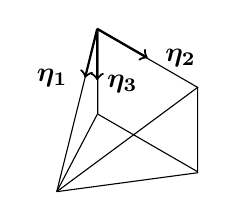
\begin{tikzpicture}[rotate=0,scale=1,shape border uses incircle,shape border rotate=-30]
  \node [name=t,shape=trapezium,draw,minimum width=2cm,
      trapezium left angle=120] at (0,0,0) {};
  
  \coordinate (punta) at (0,0,3);

  \coordinate (tl) at (t.top left corner);
  \coordinate (tr) at (t.top right corner);
  \coordinate (bl) at (t.bottom left corner);
  \coordinate (br) at (t.bottom right corner);

  \draw (tl) -- (punta);
  \draw (bl) -- (punta);
  \draw (tr) -- (punta);
  \draw (br) -- (punta);
  
  \coordinate (k1) at ($0.70*(tl) + 0.30*(punta)$);
  \coordinate (k2) at ($0.5*(tl) + 0.5*(tr)$);
  \coordinate (k3) at ($0.4*(tl) + 0.6*(bl)$);

  \node [left=1mm] (eta1) at (k1) {$\boldsymbol{\eta_1}$};
  \node [right=1mm] (eta2) at (k2) {$\boldsymbol{\eta_2}$};
  \node [below=0.5mm,right] (eta3) at (k3) {$\boldsymbol{\eta_3}$};

  \draw [->,thick] (tl) -- (k1);
  \draw [->,thick] (tl) -- (k2);
  \draw [->,thick] (tl) -- (k3);
\end{tikzpicture}
\caption{Macro--element directions in a pyramid}
\label{auxlabel8}
\end{figure}
\begin{enumerate}
  \item 
Case $E$ is a pyramid.  
Remember the local ordering for the directions
of the edges of sizes $h_1$, $h_2$ and $h_3$ for pyramids in our setting
(cfr. Figure~\ref{auxlabel8}).

As pyramids in $\Th$ don't touch singularities
and are regular, and $1-\mu\geqslant 1-\nu$, we have
\begin{IEEEeqnarray*}{rCcCl}
  \|\bu_s - \br_0\bu_s\|^2_{\sss L^2(E)} & \leqslant & h_E^2|\bu_s|_{1,E}^2
  &\leqslant&
  \textit{h}^2d(E,\be)^{2(1-\mu)}\sum_{i=1}^3 |u_{s,i}|^2_{1,E}\\
\IEEEeqnarraymulticol{5}{R}{
\begin{IEEEeqnarraybox*}{rCl}
  \qquad&\leqslant&  
    \textit{h}^2\sum_{i=1}^3\sum_{j=1}^3 \|r^{1-\mu}\gancho_{\eta_j}u_{s,i}\|_{\sss L^2(E)}^2\\
       &\leqslant&
    \textit{h}^2\left(
     \sum_{i=1}^2 \sum_{j=1}^3\|R^{1-\mu}\theta^{1-\mu}\gancho_{\eta_j}u_{s,i}\|_{\sss L^2(E)}^2
     + \sum_{j=1}^3\|R^{1-\mu}\gancho_{\eta_j}u_{s,3}\|_{\sss L^2(E)}^2\right)\\[7pt]
       &\leqslant&
    \textit{h}^2\left(
     \sum_{i=1}^2 \sum_{j=1}^3\|R^{1-\nu}\theta^{1-\mu}\gancho_{\eta_j}u_{s,i}\|_{\sss L^2(E)}^2
    + \sum_{j=1}^3\|R^{1-\nu}\gancho_{\eta_j}u_{s,3}\|_{\sss L^2(E)}^2\right)\\[7pt]
       &\leqslant&
    \textit{h}^2\left(
    \sum_{i=1}^2 \sum_{j=1}^3\|R^{\beta}\theta^{\delta}\gancho_{\eta_j}u_{s,i}\|_{\sss L^2(E)}^2+
     \sum_{j=1}^3\|R^{\beta}\gancho_{\eta_j}u_{s,3}\|_{\sss L^2(E)}^2\right)\\[7pt]
  \yesnumber\label{aux_label63} 
       &\leqslant&
    \textit{h}^2
    \|\bu_{s}\|^2_{\pazocal{V}_{\beta,\delta}(E)}.
\end{IEEEeqnarraybox*}
}
\end{IEEEeqnarray*}
\item Case $E$ is a prism (with $d(E,\be)>0$) or a tetrahedron. In the case of prisms we use 
the result of Theorem~\ref{aux_label46} and in the case of tetrahedra
we use Theorem 6.2 of~\cite{aadl}  to get
\begin{IEEEeqnarray}{rCl}\label{auxlabel9}
  \|\bu_s - \br_0\bu_s\|^2_{\sss L^2(K)}&\leqslant& C\left\{
    \sum_{i=1}^3 h_i^2\|\gancho_{\xi_i}\bu_s\|^2+
    h_K^2\|\dv\bu_s\|^2
  \right\}.
\end{IEEEeqnarray}
Now the treatment is a slight variation of the previous item including a few small
tricks. In fact,
\begin{IEEEeqnarray*}{rCcCl}
  h_1^2\|\gancho_{\xi_1}\bu_s\|^2_{L^2(E)^3}&=&
  h_1^2\sum_{i=1}^3 \|\gancho_{\xi_1}u_{s,i}\|^2_{L^2(E)}&\leqslant&
    \textit{h}^2\sum_{i=1}^3 \|r^{1-\mu}\gancho_{\xi_1}u_{s,i}\|^2_{L^2(E)}\\
\IEEEeqnarraymulticol{5}{r}{
\begin{IEEEeqnarraybox}{rCl}
\qquad&\leqslant&
    \textit{h}^2\left(
     \sum_{i=1}^2 \|R^{1-\mu}\theta^{1-\mu}\gancho_{\xi_1}u_{s,i}\|^2_{L^2(E)}+
     \|R^{1-\mu}\gancho_{\xi_1}u_{s,3}\|^2_{L^2(E)}\right)\\[7pt]
  &\leqslant&
    \textit{h}^2\left(
     \sum_{i=1}^2 \|R^{1-\nu}\theta^{1-\mu}\gancho_{\xi_1}u_{s,i}\|^2_{L^2(E)}+
     \|R^{1-\nu}\gancho_{\xi_1}u_{s,3}\|^2_{L^2(E)}\right)\\[7pt]
  &\leqslant&
    \textit{h}^2\left(
    \sum_{i=1}^2 \|R^{\beta}\theta^{\delta}\gancho_{\xi_1}u_{s,i}\|^2_{L^2(E)}+
     \|R^{\beta}\gancho_{\xi_1}u_{s,3}\|^2_{L^2(E)}\right)\\[7pt]
  &\leqslant&
    \textit{h}^2 \|\bu_{s}\|^2_{\pazocal{V}_{\beta,\delta}(E)}.
\end{IEEEeqnarraybox}
}
\end{IEEEeqnarray*}
Now, since $h_2\sim h_1$, with the same argument,
\begin{IEEEeqnarray*}{rCl}
  h_2\|\gancho_{\xi_2}\bu_s\|_{L^2(E)^3}&=&
  h_2\sum_{i=1}^3 \|\gancho_{\xi_2}u_{s,i}\|\,\leqslant\,
    \textit{h}
    \|\bu_{s}\|_{\pazocal{V}_{\beta,\delta}(E)}.
\end{IEEEeqnarray*}
For the derivative with respect to $\xi_3$ in~\eqref{auxlabel9},
\begin{IEEEeqnarray*}{rCl}
  h_3^2\|\gancho_{\xi_3}\bu_s\|^2_{L^2(E)^3}&=&
  h_3^2\sum_{i=1}^3 \|\gancho_{\xi_3}u_{s,i}\|^2_{L^2(E)}\\
\IEEEeqnarraymulticol{3}{R}{
\begin{IEEEeqnarraybox*}{rCl}
\qquad&=&h_3^2\left(\sum_{i=1}^2\|\gancho_{\xi_i}u_{s,3}\|^2_{L^2(E)}+
    \|\gancho_{\xi_3}u_{s,3}\|^2_{L^2(E)}\right)\\[7pt]
  &\leqslant&\textit{h}^2\left(\sum_{i=1}^2\|d(E,v)^{1-\nu}\gancho_{\xi_i}u_{s,3}\|^2_{L^2(E)}
      +\|d(E,v)^{1-\nu}\gancho_{\xi_3}u_{s,3}\|^2_{L^2(E)}\right)\\[7pt]
  &\leqslant&
  \textit{h}^2\left(\sum_{i=1}^2\|R^{\beta}\gancho_{\xi_i}u_{s,3}\|^2_{L^2(E)}+
    \|R^{\beta}\gancho_{\xi_3}u_{s,3}\|^2_{L^2(E)}\right)\\[7pt]
  &=&
  \textit{h}^2\sum_{i=1}^3\|R^{\beta}\gancho_{\xi_i}u_{s,3}\|^2_{L^2(E)}\\[7pt]
  &\leqslant&
  3\textit{h}^2\|u_{s,3}\|^2_{\scriptscriptstyle V^{1,2}_{\beta,0}(E)}.
\end{IEEEeqnarraybox*} 
}
\end{IEEEeqnarray*}
The divergence term in~\eqref{auxlabel9} goes like in~(\ref{aux_label64}).
\end{enumerate}
\paragraph{Terms in~\eqref{auxlabel350} such that $d(E,\be_\ell)=0$.}
In this case we have anisotropic prisms and tetrahedra from an isotropic 
subfamily, one in each tetrahedral macro--element of the present type.

From~\eqref{auxlabel350}, after triangle inequality, we write
\begin{IEEEeqnarray}{rCl} %
  \IEEEeqnarraymulticol{3}{L}{\nonumber
    \sum_{d(E,\be) = 0}
    \|\bu_s - \br_0\bu_s\|^2_{\scriptscriptstyle L^2(E)^3}
    \,\lesssim\,}
  \\
  \IEEEeqnarraymulticol{3}{R}{
  \label{distancia_cero_arista}
  \,\lesssim\,\|\br_0\bu_s\|^2_{\scriptscriptstyle L^2(T_\ell)^3}
  \,+\sum_{
  \substack{{\small{\text{prisms\,}}P}\\
          d(P,\be) = 0}} \|\br_0\bu_s\|^2_{\scriptscriptstyle L^2(P)^3}
  \,+\sum_{d(E,\be) = 0} \|\bu_s\|^2_{\scriptscriptstyle L^2(E)^3}}.
\end{IEEEeqnarray}
Here we put $T_\ell$ for the mentioned tetrahedron and
$E$ for generic elements in $\Lambda_\ell$.
Now let us bound each term.%% on the right of~(\ref{distancia_cero_arista}).
\begin{enumerate}
  \item 
  For the last term on the right of~(\ref{distancia_cero_arista}), let
$E$ be any of both the tetrahedron with the
singular
 vertex or a prism. If $E$ is a prism, recall in this case we have
 $d(E,\be) = 0$ and $d(E,\bv) > 0$. So
\begin{IEEEeqnarray*}{rCl}
   \|\bu_s\|_{L^2(E)^3} &=&
    \sum_{i=1}^2 \|R^\nu\theta^\mu R^{-\nu}\theta^{-\mu} u_{s,i}\|_{0,E}
    + \|R^\nu\theta^{-1}R^{-\nu}\theta u_{s,3}\|_{0,E}\\[7pt]
  &\leqslant&\|R^\nu\theta^\mu\|_{L^\infty(E)}
  \sum_{i=1}^2 \|R^{-\nu}\theta^{-\mu} u_{s,i}\|_{0,E}\\[4pt]
\IEEEeqnarraymulticol{3}{r}{
    +\,\|R^\nu\theta\|_{\infty,E}
    \|R^{-\nu}\theta^{-1} u_{s,3}\|_{0,E}.
}
\end{IEEEeqnarray*}
Since $\theta < 1$ and $\mu \leqslant \nu < 1$, then
\begin{IEEEeqnarray}{rClClCr}
  \label{cota_pesos}
  R(\bx)^\nu\theta(\bx)&\leqslant&
  R(\bx)^\nu\theta(\bx)^\mu&\leqslant&R(\bx)^\mu\theta(\bx)^\mu&=&
  r(\bx)^\mu.
\end{IEEEeqnarray}
Using this we get
\begin{IEEEeqnarray*}{rCl}
  \|\bu_s\|_{0,E}&\leqslant&\|r^\mu\|_{\infty,E}
  \left(
    \sum_{i=1}^2 \|R^{-\nu}\theta^{-\mu}u_{s,i}\|_{0,E}
    + \|R^{-\nu}\theta^{-1}u_{s,3}\|_{0,E}
  \right)\\[7pt]
  &\leqslant&\max\{h_1,h_2\}^\mu
  \left(
    \sum_{i=1}^2 \|R^{-\nu}\theta^{-\mu}u_{s,i}\|_{0,E}
    + \|R^{-\nu}\theta^{-1}u_{s,3}\|_{0,E}
  \right)\\[7pt]
  &\lesssim&\textit{h}
    \|\bu_{s}\|_{\pazocal{V}_{\beta,\delta}(E)}
\end{IEEEeqnarray*}
provided we take $\beta\sim 1-\nu$ and $\delta\sim 1-\mu$.
\item For the first term in~\eqref{distancia_cero_arista},
although, as we said, the tetrahedra touching the vertex remain regular, 
we estimate with 
the weighted norms anisotropically for the sake of completeness and generality.
Recall $T_\ell$ also has an edge
contained in the singular edge of $\Lambda_\ell$. %${\color{blue}\|\br_0\bu_s\|^2_{\scriptscriptstyle L^2(Tetra)^3}}$.
We work for the first component of the local interpolate in the $L^1(T_\ell)$ norm
using~(\ref{normaL2L1}).
\begin{IEEEeqnarray*}{rCl}
  \|(\br_0\bu_s)_1\|_{\scriptscriptstyle L^2(T_\ell)}
    & \leqslant & C|T_\ell|^{-1/2} \|(\br_0\bu_s)_1\|_{\scriptscriptstyle L^1(T_\ell)}.
\end{IEEEeqnarray*}
Remember that by Lemma~\ref{well_defined_dofs} we know $\bu_s$ is in 
$W^{1,1}(\Lambda_\ell)^3$. We start pulling $\br_0\bu_s$ back to a rescaled
reference tetrahedron $\tilde{T}$ 
with the mapping 
$F_{T_\ell}(\tilde{\bx}) = M_{T_\ell}\tilde{\bx} + \bx_{T_\ell}$
(cfr. Figure~\ref{rescaled_tetra}). 
\rescaledTetraTikz

Using Lemma 5.22 in page 123 of~\cite{monk},
which gives the analog of our statement in~(\ref{div_interp_commutes}) for 
tetrahedra, and then using Proposition 3.4 of~\cite{aadl}, we get
\begin{IEEEeqnarray*}{rCl}
  \|(\br_0\bu_s)_1\|_{L^1(T_\ell)} &=& \int_{\tilde{T}}|(M_{T_\ell}\tilde{\br}_0\tilde{\bu}_s)_1|\,d\tilde{\bx}\\[7pt]
    &\leqslant& C\,\bigg\{ \sum_{1\leqslant i\leqslant 3} \|\tilde{u}_{s,i}\|_{L^1(\tilde{T})} + 
      \sum_{1\leqslant j\leqslant 3} h_j\|\partial_j\tilde{u}_{s,i}\|_{L^1(\tilde{T})}\\
      \IEEEeqnarraymulticol{3}{r}{ + \,
             h_i\|\dvg \tilde{\bu}_s\|_{L^1(\tilde{T})}\bigg\}} \\[7pt] %%% & = & \ldots \text{paso al tetraedro f\'isico} \ldots \\[7pt] % VER BORRADOR INTERPOLACION PIRAMIDE
    & \leqslant & C\,
    \bigg\{\|\bu_{s}\|_{L^1(T_\ell)^3} + 
    \sum_{1\leqslant j \leqslant 3} h_j\|\partial_{\xi_j}\bu_{s}\|_{L^1(T_\ell)^3}\\
    \IEEEeqnarraymulticol{3}{r}{
    + (h_1+h_2+h_3) \|\dvg \bu_s\|_{L^1(T_\ell)}\bigg\}}\\[3pt]
&&\yesnumber\label{aux_label60}
\end{IEEEeqnarray*}
where $C$ depends only on the maximum angle of $T_\ell$. 
Now we estimate each term on the right hand side of~(\ref{aux_label60}).
\begin{enumerate}
  \item[(2a)] By H\"older's inequality
\begin{IEEEeqnarray*}{rCl}
  \|\bu_{s}\|_{L^1(T_\ell)^3} &\leqslant&
\sum_{i=1,2}\|R^{\nu}\theta^{\mu}\|_{L^2(T_\ell)}\|R^{-\nu}\theta^{-\mu}u_{s,i}\|_{L^2(T_\ell)}\\ %%&\leqslant&\|R^\nu\theta^{\mu}\|_\infty|T_\ell|^{\nicefrac12}\sum_{i=1,2}\|\ldots u_{s,i}\|_{L^2(T\ell)} + \|R^\nu\theta\|_\infty|T_\ell|^{\nicefrac12}\|\ldots u_{s,3}\|_{L^2(T\ell)}\\[7pt]
 & &\qquad+\,\|R^{\nu}\theta\|_{L^2(T_\ell)}\|R^{-\nu}\theta^{-1}u_{s,3}\|_{L^2(T_\ell)}
\end{IEEEeqnarray*}
and by~(\ref{cota_pesos}) and the grading criterion~(\ref{label_grading}) we have                                        %&\leqslant&(\textit{h}^{1/\mu})^\mu|T_\ell|^{\nicefrac12}\sum_{i=1,2}\|R^{-\nu}\theta^{-\mu}u_{s,i}\|_{L^{2}(T_\ell)} +\|R^{-\nu}\theta^{-1} u_{s,3}\|_{L^{2}(T_\ell)}\\[7pt]
\begin{IEEEeqnarray*}{rCl} 
\|\bu_{s}\|_{L^1(T_\ell)^3} &\leqslant&(\textit{h}^{1/\mu})^\mu|T_\ell|^{\nicefrac12}
\|\bu_s\|_{V_{\beta,\delta}^{1,2}(T_\ell)^2\times V_{\beta,0}^{1,2}(T_\ell)}\\
&=&\textit{h}\,|T_\ell|^{\nicefrac12}\|\bu_s\|_{\pazocal{V}_{\beta,\delta}(T_\ell)}.
\end{IEEEeqnarray*}
  \item[(2b)]
Take $1\leqslant j,i \leqslant 3$. Then %%% TODO (HACER APARTE PARA $i=3$; creo que es un poco diferente, como pas\'o antes):
\begin{IEEEeqnarray*}{rCl}
  h_j\|\partial_{\xi_j} u_{s,i}\|_{L^1(T_\ell)} & \leqslant &
    h_j\|R^{\nu-1}\theta^{\mu-1}\|_{0,T_\ell}\|R^{1-\nu}\theta^{1-\mu}\partial_{\xi_j} u_{s,i}\|_{0,T_\ell}.
\end{IEEEeqnarray*}
As it holds $0\leqslant1-\nu\leqslant1-\mu<1$, we get 
\[
  R(\bx)^{1-\nu}\geqslant R(\bx)^{1-\mu}
\]
and
\[
  R(\bx)^{\nu-1}\theta(\bx)^{\mu-1}\leqslant
  R(\bx)^{\mu-1}\theta(\bx)^{\mu-1} = r(\bx)^{\mu-1}.
\]
From this we will use that
\[
  \|R^{\nu-1}\theta^{\mu-1}\|_{L^2(T_\ell)} \leqslant \|r^{\mu-1}\|_{L^2(T_\ell)}.
\]
Now, calculating the right hand side integrating in a cylindrical section,
\[
  \|r^{\mu-1}\|_{L^2(T_\ell)} = \sqrt{\tfrac{\pi}{4\mu}}\sqrt{h_3}\,h_1^{\mu}\sim \sqrt{h_3}\,\textit{h}.
\]
Then
\begin{IEEEeqnarray*}{rCl}
  h_j\|r^{\mu-1}\|_{L^2} & \lesssim & \sqrt{h_1h_2h_3}\,\textit{h}\\[7pt]
    & \sim & \sqrt{|T_\ell|}\,\textit{h}
\end{IEEEeqnarray*}
and then
\begin{IEEEeqnarray}{rCl}
\nonumber
  h_j\|\partial_{\xi_j} u_{s,i}\|_{L^1(T_\ell)} & \lesssim &
    \textit{h}\,\sqrt{|T_\ell|}\,\|R^{1-\nu}\theta^{1-\mu}\partial_{\xi_j} u_{s,i}\|_{L^2(T_\ell)}\\
\label{cuentita_integral}
    &\leqslant& \textit{h}\,\sqrt{|T_\ell|}\,\|u_{s,i}\|_{\scriptscriptstyle V^{1,2}_{\beta,\delta}(T_\ell)}.
\end{IEEEeqnarray}
\item[(2c)]\label{aux_label65} For the divergence term in~(\ref{aux_label60}):
\begin{IEEEeqnarray*}{rClCr}
  (h_1+h_2+h_3) \|\dvg \bu_s\|_{L^1(T_\ell)} & \leqslant &
    (2\textit{h}^{1/\mu} + \textit{h}^{1/\nu}) \|\dvg \bu_s\|_{L^1(T_\ell)} \\[7pt]
\IEEEeqnarraymulticol{3}{r}{
  \begin{IEEEeqnarraybox*}{rCl}
    & \leqslant & 3\,\textit{h}\,\sqrt{|T_\ell|}\,\|\dvg \bu_s\|_{L^2(T_\ell)} 
    \\[7pt]
    & \leqslant & 3\,\textit{h}\,\sqrt{|T_\ell|}\,\left\{\|\dv\bu\|_{L^2(T_\ell)}
     + \|\dv\bu_r\|_{L^2(T_\ell)}\right\}.
  \end{IEEEeqnarraybox*}
}\\&&
\yesnumber\label{aux_label66}
\end{IEEEeqnarray*}
\end{enumerate}
\item 
Now prisms, the middle term on the right hand of~(\ref{distancia_cero_arista}). Remember
the difference with the tetrahedron is that $d(P,\bv_\ell) \gtrsim h_1$.
We start pulling back from $P$ to the rescaled prism in Figure~\ref{rescaled_prism}
called here $\tilde P$.   
By the stability estimate in Theorem~\ref{thmStabilityKtildeRT}, 
\begin{IEEEeqnarray*}{rCl}
  \|\br_0\bu_s\|_{\scriptscriptstyle L^1(P)^3} & \leqslant & 
    \|M_P\|_\infty \|\tilde{\br}_0\tilde{\bu}_s\|_{L^1({\tilde{P}})^3} \\ [7pt]
\IEEEeqnarraymulticol{3}{r}{
\begin{IEEEeqnarraybox*}{rCl}
 \qquad&\lesssim& \left\| \tilde{\bu}_s \right\|_{L^1(\tilde{P})^3}
    + \sum_{j=1}^3 h_j \left\| \partial_{\tilde{x}_j}\tilde{\bu}_s \right\|_{L^1(\tilde{P})^3}
    + h_{\tilde{P}}\left\|\dv(\tilde{u}_{s,1}, \tilde{u}_{s,2}, 0) \,\right\|_{L^1(\tilde{P})}\\[7pt]
  &\lesssim& \left\| \bu_s \right\|_{L^1(P)^3}
    + \sum_{j=1}^3 h_j \left\| \partial_{\xi_j}\bu_s \right\|_{L^1(P)^3}
    + h_{P}\left\|\dv(u_{s,1}, u_{s,2}, 0) \,\right\|_{L^1(P)}\mbox{,}    
\end{IEEEeqnarraybox*}
}\\[4pt]
&&\yesnumber\label{auxlabel10}
\end{IEEEeqnarray*}
by the same argument as in~(\ref{aux_label15}) for 
elements touching the singular edge in the prismatic macro--element. Now
to estimate each term, again for $i=1$ or $2$ we have
\begin{IEEEeqnarray*}{rCcCl}
  \|u_{s,i}\|_{L^1(P)} & \leqslant & 
    \|R^{\nu}\theta^{\mu}\|_{0,P} \|R^{-\nu}\theta^{-\mu}u_{s,i}\|_{0,P}
      & \leqslant & \textit{h}\,|P|^{\nicefrac12} \|R^{-\nu}\theta^{-\mu}u_{s,i}\|_{0,P}
\end{IEEEeqnarray*}
and
\begin{IEEEeqnarray*}{rCcCl}
  \|u_{s,3}\|_{L^1(P)} & \leqslant & \|R^{\nu}\theta\|_{0,P} \|R^{-\nu}\theta^{-1}u_{s,3}\|_{0,P}
  & \leqslant & \textit{h}\,|P|^{\nicefrac12} \|R^{-\nu}\theta^{-1}u_{s,3}\|_{0,P}.
\end{IEEEeqnarray*}
Next fix $j = 1$ or $2$.         %\noindent DErivatives: $j = 1$ or $2$.\\
If $i=1$ or $2$, with the same argument as in~(\ref{cuentita_integral}), we state that
\begin{IEEEeqnarray}{rCl}
  h_j\|\partial_{\xi_j} u_{s,i}\|_{L^1(P)} & \lesssim &
    \textit{h}\,\sqrt{|P|}\,\|R^{1-\nu}\theta^{1-\mu}\partial_{\xi_j} u_{s,i}\|_{0,P}.
\end{IEEEeqnarray}
For the derivatives of $u_{s,3}$ it holds that 
\begin{IEEEeqnarray*}{rCl}
  h_j\|\partial_{\xi_j}u_{s,3}\|_{L^1(P)} &\leqslant&
    h_j \|R^{\nu-1}\|_{0,P}\|R^{1-\nu}\partial_{\xi_j}u_{s,3}\|_{0,P}\\[7pt]
  &\leqslant& h_j \|r^{\mu-1}\|_{0,P}\|R^{1-\nu}\partial_{\xi_j}u_{s,3}\|_{0,P}\\[7pt]
  &\lesssim& \textit{h}\,\sqrt{|P|}\,\|R^{1-\nu}\partial_{\xi_j}u_{s,3}\|_{0,P}.
\end{IEEEeqnarray*}
Now, for the  derivative along the direction of the singular edge 
$\partial_{\xi_3}(\cdot)$, remember in this case it is 
$h_3\sim\textit{h}\,d(P,\bv)^{1-\nu}$. If we take first and second components,
\begin{IEEEeqnarray*}{rCl}
  h_3\|\partial_{\xi_3}u_{s,i}\|_{L^1(P)}& = & h_3\|\partial_{\xi_i}u_{s,3}\|_{L^1(P)}\\[7pt]
  & \leqslant & C\textit{h}\|R^{1-\nu}\partial_{\xi_i}u_{s,3}\|_{L^1(P)}\\[7pt]
  & \leqslant & C\textit{h}|P|^{\nicefrac12}\|R^{1-\nu}\partial_{\xi_i}u_{s,3}\|_{L^2(P)}.
\end{IEEEeqnarray*}
And if we take the third component,
\begin{IEEEeqnarray*}{rCl}
  h_3\|\partial_{\xi_3}u_{s,3}\|_{L^1(P)}& \sim & \textit{h}\|d(P,\bv)^{1-\nu}
    \partial_{\xi_3}u_{s,3}\|_{L^1(P)}\\[7pt]
  & \leqslant & C\textit{h}\|R^{1-\nu}\partial_{\xi_3}u_{s,3}\|_{L^1(P)}\\[7pt]
  & \leqslant & C\textit{h}|P|^{\nicefrac12}\|R^{1-\nu}\partial_{\xi_3}u_{s,3}\|_{L^2(P)}.
\end{IEEEeqnarray*}
For the divergence term in~\eqref{auxlabel10},
\begin{IEEEeqnarray*}{rCl}
  h_P\|\dv(u_{s,1},u_{s,1},0)\|_{L^1(P)}&\leqslant&h_P\|\dv\bu_s\|_{L^1(P)}
    +h_P\|\partial_{\xi_3}u_{s,3}\|_{L^1(P)}\\[7pt]
    &\lesssim&h_P\|\dv\bu_s\|_{L^1(P)} + h_3\|\partial_{\xi_3}u_{s,3}\|_{L^1(P)}\mbox{;}
\end{IEEEeqnarray*}
the estimate for $h_P\|\dv\bu_s\|_{L^1(P)}$ follows as in~(\ref{aux_label66}), 
and the estimate for $h_3\|\partial_{\xi_3}u_{s,3}\|_{L^1(P)}$ should be
\begin{IEEEeqnarray*}{rCl}
  h_3\|\partial_{\xi_3}u_{s,3}\|_{L^1(P)} & \lesssim &
  \textit{h} |P|^{\nicefrac12}\|R^{1-\nu}\partial_{\xi_3}u_{s,3}\|_{L^2(P)} \\
  &\lesssim& \textit{h} |P|^{\nicefrac12}\|u_{s,3}\|_{V_{\beta,0}(P)}.
\end{IEEEeqnarray*}
\end{enumerate}
Collecting all the estimates in items $2$ and $3$ above, using~(\ref{normaL2L1})
we bound the first and second term in~(\ref{distancia_cero_arista}), 
belonging to the case with zero distance
to the edge, in the $L^2$ norm.

\subsection{Bound for the Singular Part in a Tetrahedral Macro--Element
with Singular Vertex and no Singular Edge}
This macroelement is made up with a graded subfamily of isotropic tetrahedra.
The grading fulfills the relations~\eqref{label_grading2} and the estimates
follow repeating (in fact, simpler) arguments used in Subsection~\ref{auxlabel205}.  
%% {\color{blue}\# continue here; anotar para seguir 
%% en el remark del caso de macroel. que me marcó ariel que faltar'ia 
%% (ver mi cuaderno)}

\section{examples of the meshing procedure} % (fold)
\label{sec:examples_of_the_meshing_procedure}

% section examples_of_the_meshing_procedure (end)


\chapter{Further Results on Finite Elements}
\section{An\-iso\-tropic Stability Estimates for $H(\bcurl)$ Conforming Finite
Elements on Prisms}
\label{stab_edge_prism}
We are writing the following three Lemmas which state some special
behavior of the interpolation operator, mostly related to the preservation of
null components of the fields, and whose proofs consist in a smart use of the
degrees of freedom and the very definition of the operator. These Lemmas, 
although just with technical purpose, exhibit
nice properties of the interpolators.

In the present subsection $\hat\bu$ is an element
in $W^{1,p}(\hat{E})$ for $p>2$ which is a space whose elements have well
defined tangential traces on each edge of the prism $\hat{E}$.
Another possibility, as stated in Lemma $5.38$ in the page $134$ of~\cite{monk},
is to assume there are 
a positive $\delta$ and a $p>2$ such that 
$\hat\bu$ belongs to $H^{1/2+\delta}(\hat{E})^3$ and
${\bf curl}\,\bu$ belongs to $L^p(\hat{E})^3$.
For the whole section, $\hat\bw_k$ will be the $k$--th order edge 
interpolation operator on the reference
Prism determined by the element of
\emph{Definition}~\ref{edgeelement}.

\begin{lemma}\label{lema_PIu3_k_cualquiera} 
$(\wku)_3$ is linearly and univocally 
determined by $\hat{u}_3$.
\end{lemma}
\begin{proof} If we pay attention to the directions of the unit
tangents and normals to the edges and faces, respectively, of $\hat E$,
we realize that
the degrees of freedom which involve $(\wku)_3$ give rise only to the 
following linear equations
\begin{IEEEeqnarray}{rCrc}
\varphi_{\hat{\be}_i,p}\,(\wku) & = & \varphi_{\hat{\be}_i,p}\,(\hat{\bu}) &\quad\mbox{as in~(\ref{momentos1hcurl}) for $i$ = 3, 6, 7,}\\
\varphi_{f_1,\bq}\,(\wku) & = & \varphi_{f_1,\boldsymbol{q}}\,(\hat{\bu})
  &\quad\mbox{as in~(\ref{momentos3hcurl})}\\
\varphi_{f_2,\bq}\,(\wku) & = & \varphi_{f_2,\boldsymbol{q}}\,(\hat{\bu})
  &\quad\mbox{as in~(\ref{momentos4hcurl})}  \\
\varphi_{f_5,\bq}\,(\wku) & = & \varphi_{f_5,\boldsymbol{q}}\,(\hat{\bu})
  &\quad\mbox{as in~(\ref{momentos5hcurl})}  \\
\varphi_{\boldsymbol{r}}\,(\wku) & = & \varphi_{\boldsymbol{r}}\,(\hat{\bu})
  &\quad\mbox{as in~(\ref{momentos6hcurl})}.
\end{IEEEeqnarray}
These are 
$3k$+$3k(k-1)$+$k(k-1)(k-2)/2 = k(k+1)(k+2)/2$ equations,
just the dimension of $P_k(\hat{T})\otimes P_{k-1}(\hat{I})$, 
which is the space $(\wku)_3$ belongs to by definition.
%$\frac{k(k+1)(k+2)}{2}$. 
%libertad en los que no des\-a\-pa\-re\-ce $(\wku)_3$ son \'unicamente:
Now set all those equations equal to zero (that is, pick $u_3 = 0$) and see that
the unique solution is $(\wku)_3 = 0$.
A little more explicitly, we have:
\begin{IEEEeqnarray}{lCll}
  \label{aristas} \int_{\hat\be_i} (\wku)_3\,\hat q \, d\alpha 
  & = & 0 &\qquad \mbox{for $i$ = 3, 6 and 7, }q\in P_{k-1}(\hat\be_i)\\[5pt]
  \label{caras} \iint_{\hat f_j} (\wku)_3\,\hat q \,d\hat S
  & = & 0 &\qquad \mbox{for $j$ = 1, 2, and 5, } \hat q\in Q_{k-2,k-1}(\hat f_j)\\[5pt]
  \label{enK} \int_{\hat{E}} (\wku)_3\,\hat q_3 \, d\bx 
  & = & 0 &\qquad \mbox{for }\hat q_3\in P_{k-3,k-1}.
\end{IEEEeqnarray}
Start considering the face $\hat f_2$.
The restriction of $(\wku)_3$ to $\be_3$
is itself 
an element in $P_{k-1}({\be_3})$, 
and the same holds for $\be_6$,  
so equations~(\ref{aristas}), for $i = 3$, $6$, say that $(\wku)_3$
is identically null on those edges by which
the restriction 
$(\wku)_3|_{f_2}$, which is an element of $P_k(\hat x_1)\otimes P_{k-1}(\hat x_3)$
may be se factorized
as
$(\wku)_3|_{f_2}(\hat x_1,0,\hat x_3) = \hat x_1\,(1-\hat x_1)\,w_0(\hat x_1,\hat x_3)$,
with $w_0$ equal to some polynomial in $P_{k-2}(\hat x_1) \otimes P_{k-1}(\hat x_3)$.
Now choose $\hat q = w_0$ in the degrees of freedom~(\ref{caras}) for the face
$\hat f_2$ and it holds
\begin{IEEEeqnarray}{lClc}
	\iint_{\hat f_2} \hat{x}_1(1-\hat{x}_1)w_0(\hat{x}_1,\hat{x}_3)^2\,d\hat S & = & 0.
\end{IEEEeqnarray}
But $\hat{x}_1\,(1-\hat{x}_1)$ is almost everywhere positive over the closure
of $\hat f_2$, so 
$(\wku)_3|_{\hat f_2}$ vanishes identically.
By a completely symmetric observation we can prove 
$(\wku)_3|_{\hat f_1} \equiv 0$.\\
One more time, if we use~(\ref{aristas}) for $i =$ 6, 7,
$\hat x_1\,(1-\hat x_1)$ divides the restriction $(\wku)_3|_{\hat f_5}$, so that
there is a 
$w_1 \in P_{k-2}(\hat x_1)\otimes P_{k-1}(\hat x_3)$ for which 
$(\wku)_3|_{\hat f_5}(\hat x_1, \hat x_2, \hat x_3) = \hat{x}_1\,\displaystyle{(1-\hat{x}_1)}\,w_1(\hat{x}_1,\hat{x}_3)$.
Now equality~(\ref{caras}) for $j = 5$ implies
$(\wku)_3|_{f_5} \equiv 0$.\\
Next, since $(\wku)_3$ vanishes when restricted $\hat f_1$, $\hat f_2$ and $\hat f_5$
we get to factorize it on $\hat E$ as 
\begin{IEEEeqnarray*}{rCl}
	(\wku)_3(\hat x_1, \hat x_2, \hat x_3) 	& = 	& \hat{x}_1\,\hat{x}_2\,(1-\hat{x}_1-\hat{x}_2)\,w_3(\hat{x}_1,\hat{x}_2,\hat{x}_3),\\
									w_3		& \in 	& P_{k-3}(\hat x_1)\otimes P_{k-1}(\hat x_3).
\end{IEEEeqnarray*}
And now we evaluate the degrees of freedom~(\ref{enK}) choosing
$\hat q_3 \equiv w_3$ and conclude immediately
$(\wku)_3 \equiv 0$ on $\hat E$. 
\end{proof}
\label{auxlabel500}
\begin{lemma}\label{auxlabel501}
\begin{itemize}
	\item []
	\item [(a)] If $\hat\bu(\hat x_1,\hat x_2,\hat x_3) = (0, \hat u_2(\hat x_2,\hat x_3), 0)'$,
	then 
  \[
  \wku\xyz = (0, \hat\xi_2(\hat x_2,\hat x_3) ,0)'
  \]
  for some 
	$\hat\xi_2 \in P_{k-1}(\hat{x}_2) \otimes P_k(\hat{x}_3)$.
	\item [(b)]\label{piu1_k_in_N} If $\hat\bu(\hat x_1,\hat x_2,\hat x_3) = (\hat u_1(\hat x_1,\hat x_3), 0, 0)'$
	then
  \[
  \wku\xyz = (\hat\xi_1(\hat x_1,\hat x_3), 0 ,0)'
  \]
  for some
    $\hat\xi_1\in P_{k-1}(\hat{x}_1) \otimes P_k(\hat{x}_3)$.
\end{itemize}
\end{lemma}
\begin{proof} We will prove the first inequality, as the second follows
with the same ideas. In Subsection~\ref{sub:defEdgeElement} we found 
expression~(\ref{elemento_P_k}) which states
\begin{IEEEeqnarray*}{rCl}
  \wku\xyz  & = & (p_1\xyz, p_2\xyz, p_3\xyz)^t\\[4pt]
  			    & = & \begin{pmatrix}
  					        \xi_1\xyz + \hat{x}_2\,h\xyz\\
                    \yesnumber\label{expr_wku}\xi_2\xyz - \hat{x}_1\,h\xyz \\
  					        \xi_3\xyz
  				        \end{pmatrix}
\end{IEEEeqnarray*}
for
$\xi_1$ and $\xi_2$ in $P_{k-1}(\hat{f}_3) \otimes P_k(\hat{x}_3)$,
$\xi_3$ in $P_{k}(\hat{f}_3) \otimes P_{k-1}(\hat{x}_3)$,
and $h$ in $\tilde{P}_{k-1}(\hat{f}_3) \otimes P_k(\hat{x}_3)$.
Thanks to Lemma~\ref{lema_PIu3_k_cualquiera} we already know that $\xi_3 \equiv 0$,
so we are going to show
that $h \equiv 0$, $\xi_1 \equiv 0$ and that $\xi_2$ does not depend 
on $\hat{x}_1$. First, if $\hat{f}$ is either $\hat{f}_3$ o $\hat{f}_4$, then
with a direct calculation we see that $({\bf curl}\,\wku)_3 |_{\hat f}$ belongs to
$P_{k-1}(\hat{f})$. By the commutative diagram property expressed
in~(\ref{curl_commutativity}), the definition of the degrees of freedom~(\ref{momentos1hdiv})
and the interpolation operator $\br_{\hat E}$
in Definition~\ref{defi_face_element}, it holds that, if $\hat{f}$ is 
either $\hat{f}_3$ or $\hat{f}_4$, then for every $q \in P_{k-1}(\hat{f})$,
\begin{IEEEeqnarray*}{rCCCl}
  \hat\rho_{\hat{f},q}\,({\bf curl\,}\wku)
  & = & \hat\rho_{\hat{f},q} (\br_{\hat E}\,{\bf curl\,}\hat\bu) &&\\[5pt]
  & = & \iint_{\hat f} ({\bf curl\,}\hat \bu)_3\,q \,d\hat S & = & 0.	
\end{IEEEeqnarray*}
As is for time being expected, the choice $q = ({\bf curl}\,\wku)_3 |_{\hat{f}}$
yields 
\[
  ({\bf curl}\,\wku)_3 |_{\hat{f}} \equiv 0
\]
so we may write again $(\curl \wku)_3 = \hat{x}_3\,(\hat{x}_3-1)\,\hat\psi$ for
a $\hat\psi\in P_{k-1}(\hat{f}) \otimes P_{k-2}(\hat{x}_3)$.
We choose now $q=\hat\psi$ in the degrees of freedom~(\ref{momentos4hdiv}).
By the commutative diagram property
and the definition of $\br_{\hat E}$, we have 
\begin{IEEEeqnarray*}{rCCCl}
	\int_{\hat{E}} \hat{x}_3\,(\hat{x}_3-1)\,\hat\psi^2\,d\hat{\bx}
  & = &\int_{\hat{E}} (\curl\wku)_3\,\hat\psi\,d\hat{\bx}&&\\
  & = &\int_{\hat{E}} (\br_{\hat E}\curl\hat{\bu})_3\,\hat{\psi}\,d\hat{\bx}&&\\
  & = &\int_{\hat{E}} (\curl\hat{\bu})_3\,\hat{\psi}\,d\hat{\bx} & = & 0\\
\end{IEEEeqnarray*}
and it follows that
\begin{IEEEeqnarray}{rCl}
	\label{rot_3_es_0} (\curl\wku)_3 &\equiv& 0.
\end{IEEEeqnarray}
Now if we explore $({\bf curl}\,\wku)_3$ taking derivatives in  
expression~(\ref{expr_wku}) we get 
\begin{IEEEeqnarray*}{rCl}
  (\curl\wku)_3 & = & 
  \dfrac{\partial}{\partial \hat x_1}(\wku)_2 - \dfrac{\partial}{\partial \hat x_2}(\wku)_1\\[5pt]
  \label{expre_h} \yesnumber & = & -(2\,h + \hat{x}_2\,\dfrac{\partial h}{\partial \hat{x}_2} + 
	\hat{x}_1\,\dfrac{\partial h}{\partial \hat{x}_1}) + 
	\dfrac{\partial\hat\xi_2}{\partial \hat{x}_1} - \dfrac{\partial\hat\xi_1}{\partial \hat{x}_2}.
\end{IEEEeqnarray*}
Observing the degrees in each term, there hold
\begin{enumerate}
  \item 
  $g\,:=\,2\,h + \hat{x}_2\,\dfrac{\partial h}{\partial \hat{x}_2} + 
  \hat{x}_1\,\dfrac{\partial h}{\partial \hat{x}_1}
  \mbox{ belongs to } \tilde{P}_{k-1}(\hat{f}_3) \otimes P_k(\hat x_3)$
  \item 
  $\dfrac{\partial\hat\xi_2}{\partial \hat{x}_1} -
  \dfrac{\partial\hat\xi_1}{\partial \hat{x}_2}
  \mbox{ belongs to } P_{k-2}(\hat{f}_3) \otimes P_k(\hat x_3)\mbox{,}$
\end{enumerate}
but from this it follows necessarily that $g \equiv 0$. Now, how do the terms
of $g$ look like? Let us put
\begin{IEEEeqnarray*}{rCl}
	h\xyz &=& \sum_{\stackrel{i+j\,=\,k-1}{l\,\leqslant\,k}} \alpha_{_{i,j,l}}\,\hat{x}_1^i \hat{x}_2^j \hat{x}_3^l.
\end{IEEEeqnarray*}
Then
\begin{IEEEeqnarray*}{rCl}
  g\xyz & = & \sum_{\stackrel{i+j\,=\,k-1}{l\,\leqslant\,k}} 
  (2\alpha_{_{i,j,l}} + j\,\alpha_{_{i,j,l}} + i\,\alpha_{_{i,j,l}}) \hat{x}_1^i \hat{x}_2^j \hat{x}_3^l\\
  \yesnumber\label{h_is_zero} & = &(k+1)\,h\xyz\,=\,0,
\end{IEEEeqnarray*}
so $h \equiv 0$ too and, for now, 
\begin{IEEEeqnarray*}{rCl}
\wku\xyz &=& 
(\hat\xi_1\xyz, \hat\xi_2\xyz, 0)'. 
\end{IEEEeqnarray*}
The second--to--last task is to see that $\hat\xi_1$ vanishes identically.
We turn back to de edge degrees of freedom.
Set $\be$ equal to $\hat\be_1$ or $\hat\be_4$. Then the restriction
$\hat\xi_1|_{\be}$ belongs to $P_{k-1}(\be)$, so letting $\hat q = \hat\xi_1|_{\be}$ in
~(\ref{momentos1hcurl}) we obtain
\begin{IEEEeqnarray*}{rCCCCCl}
	0 &=& \hat\varphi_{\be,\,\hat\xi_1}\,(\hat\bu) &=&
	\hat\varphi_{\be,\,\hat\xi_1}\,(\wku) &=& \int_{\be} (\hat\xi_1)^2\,d\alpha\textrm{,}
\end{IEEEeqnarray*}
so, for some $\hat{p} \in P_{k-1}(\hat x_1)\otimes P_{k-2}(\hat x_3)$ we have
\[
  \hat\xi_1|_{\hat f_2}(\hat x_1,\hat x_3) = \hat{x}_3\,(\hat{x}_3-1)\,\hat{p}(\hat x_1,\hat x_3).
\]
Next choose $\hat{f} = \hat{f}_2$ and $\boldsymbol{q}=(0,0,\hat{p})'$ in~(\ref{momentos4hcurl}).
\begin{IEEEeqnarray*}{rCCCCCl} 
  0 & = & \hat\varphi_{\hat{f}_2,\bq}\,(\hat\bu) 
    & = & \hat\varphi_{\hat{f}_2,\bq}\,(\wku) 
    & = & \iint_{\hat{f}_2} \hat{x}_3\,(\hat{x}_3-1)\hat{p}^2\,d\hat S.
\end{IEEEeqnarray*}
It follows that $\hat\xi_1|_{\hat f_2}\equiv 0$, by which we know it exists
certain $\zeta \in P_{k-2}(\hat{f}_3)\otimes P_k(\hat{x}_3)$ satisfying
\[
\hat\xi_1\xyz = \hat{x}_2\,\zeta\xyz.
\]
Now we switch to the faces $\hat{f} = \hat{f}_3$ or $\hat{f}_4$. 
Take $\hat{\boldsymbol{q}} = (\zeta|_{\hat f},0,0)'$ in~(\ref{momentos2hcurl})
\begin{IEEEeqnarray*}{rCCCCCl}
  0 & = & \varphi_{\hat f,\hat{\boldsymbol{q}}}\,(\hat\bu) 
    & = & \varphi_{\hat f,\hat{\boldsymbol{q}}}\,(\wku) 
    & = & \iint_{\hat f} \hat{x}_2\zeta^2\,d\hat S\textrm{,}
\end{IEEEeqnarray*}
and it follows that
$\hat{x}_3\,(\hat{x}_3-1)$ divides $\zeta$. So putting this together
with the previous factorization, there is some
$r \in P_{k-2}(\hat{f}_3)\otimes P_{k-2}(\hat{x}_3)$ which satisfies.
\begin{IEEEeqnarray*}{rCl}
    \hat\xi_1\xyz &=& \hat{x}_2\,\hat{x}_3\,(\hat{x}_3-1)\,r\xyz.
\end{IEEEeqnarray*}
It remains to use the volume degrees of freedom. We could choose
 $\hat\br := (r,0,0)'$ in degree of freedom~(\ref{momentos6hcurl})
to get
\begin{IEEEeqnarray*}{rCCCCCl}
  0 & = & \hat\varphi_{\hat\br}\,(\hat{\bu}) & = & \hat\varphi_{\hat\br}\,(\wku)
    & = & \int_{\hat{E}} \hat{x}_2\,\hat{x}_3\,(\hat{x}_3-1)\,r\xyz^2\,d\hat\bx\textrm{,} 
\end{IEEEeqnarray*}
which yields, over all $\hat{E}$, $\hat\xi_1  \equiv  0$. Finally, if we
combine this last property with~(\ref{rot_3_es_0}) we prove that $\hat{\xi}_2$
does not depend on $\hat{x}_2$.
\end{proof}
\begin{lemma}\label{pi00u3} 
If $\hat{\bu}\xyz=(0,0, \hat{u}_3\xyz)^t$, then
$\wku\xyz = (0,0,\hat\xi_3\xyz)^t$ for some
$\hat\xi_3 \in {P}_k(\hat{f}_3)\otimes
{P}_{k-1}(\hat{x}_3)$.
\end{lemma}
\begin{proof} We will work again with
expression~(\ref{expr_wku}).
%but we will write with less details than in the previous two Lemmas
By expression~(\ref{expre_h}) for $(\curl\wku)_3$
and the commutativity in equation~(\ref{curl_commutativity}),
if we apply degrees of freedom~(\ref{momentos1hdiv})
to $\curl\hat\bu$ we obtain that
$(\curl\wku)_3$ vanishes on any of the horizontal faces $\hat{f}_3$ or $\hat{f}_4$ in
Table~\ref{prismNotationTableFaces}.
In other words, $(\curl\wku)_3
= \hat{x}_3\,(\hat{x}_3-1)\,\hat\psi$, 
($\hat\psi\in P_{k-1}(\hat{f}_3)\otimes P_{k-2}(\hat{x}_3)$)
and if we set $\hat{\br} := (0,0,\hat\psi)'$ in the
$H(\mbox{div})$ degrees of freedom~(\ref{momentos4hdiv})
we have
\begin{IEEEeqnarray*}{rCCCCCCCl}
0 & = & \int_{\hat{E}} (\curl\hat{\bu})_3\,\hat{\psi}
  & = & \hat\rho_{\br} (\curl\hat{\bu})
  & = & \hat\rho_{\br} (\hat{\br}_k\curl\hat{\bu})
  & = & \hat\rho_{\br} (\curl\wku)\\[4pt]
  &&&&&&& = & \int_{\hat{E}} \hat{x}_3(1-\hat{x}_3)\hat{\psi}^2\,d\bx
\end{IEEEeqnarray*}
yielding that $\hat\psi$ is identically zero, and also
$(\curl\wku)_3$ is identically zero.

From this point, if
we copy the argument in the proof of
Lemma~\ref{auxlabel500} starting with equation~(\ref{expre_h}) we arrive at
$h\equiv 0$, so we may rewrite~(\ref{expr_wku}) for the present case as
\begin{IEEEeqnarray}{rCl}
  \label{expre_pi00u3_} \wku &=&
  (\hat\xi_1,\hat\xi_2,\hat\xi_3)^t.
\end{IEEEeqnarray}
We claim that $\hat{\xi}_1\equiv\hat{\xi}_2\equiv0$.
To see this, first observe that the evaluation of the degrees of freedom
for the edges $\hat\be_1$ and $\hat\be_2$ yields
$\hat\xi_1|_{\hat\be_1} \equiv \hat\xi_2|_{\hat\be_2} \equiv 0$,
hence, evaluating the degree of freedom~(\ref{momentos2hcurl})
tangent to the face $\hat{f}_3$ two times we have
$\hat\xi_1|_{\hat{f}_3}  \equiv  \hat\xi_2|_{\hat{f}_3}  \equiv  0$.
In equal manner, if we pick $\hat\be_4$ and $\hat\be_5$, and then the 
degree of freedom tangent to $\hat{f}_4$ we obtain
$\hat\xi_1|_{\hat{f}_3} \equiv \hat\xi_2|_{\hat{f}_3} \equiv  0$.
So we proved there are polynomials $p_1$ and $p_2$ in
$P_{k-1}(\hat{f}_3)\otimes P_{k-2}(\hat{x}_3)$ which allow us to write
\begin{IEEEeqnarray*}{rCl}
  \hat\xi_1\xyz & = & \hat{x}_3(1-\hat{x}_3)p_1\xyz\\[4pt]
  \hat\xi_2\xyz & = & \hat{x}_3(1-\hat{x}_3)p_2\xyz.
\end{IEEEeqnarray*}
Take $\hat\bq := (0,0, \hat{q}_2|_{\hat{f}_2})'$ and 
evaluate the degree of freedom~(\ref{momentos3hcurl}). We have
\begin{IEEEeqnarray*}{rCCCCCl}
  0 & = & \hat\varphi_{\hat{f}_1,\hat{\bq}}\,(\hat\bu) 
    & = & \hat\varphi_{\hat{f}_1,\hat{\bq}}\,(\wku) 
    & = & \iint_{\hat{f}_1} \hat{x}_3(1-\hat{x}_3)\hat{q}_2^2\,d\hat S.
\end{IEEEeqnarray*}
Hence, there is some $\hat{r}_2\in P_{k-2}(\hat{f_3})\otimes P_{k-2}(\hat{x}_3)$
such that $\hat\xi_2 = \hat{x}_1\hat{x}_3(1-\hat{x}_3)\hat{r}_2$.
Now choose $\br = (0,\hat{r}_2,0)'$ and use degree of freedom~(\ref{momentos6hcurl})
to obtain $\int_{\hat{E}}\hat{x}_1\hat{x}_3(1-\hat{x}_3)\hat{r}_2^2\,d\hat\bx=0.$
Since 
$\hat{x}_1\hat{x}_3(1-\hat{x}_3)\hat{r}_2^2$ is almost everywhere greater than zero,
this implies
$\hat{\xi}_2 = 0$.
With the simmetric procedure starting with face $\hat f_2$ we get to prove
$\hat{\xi}_1 = 0$.
\end{proof}
Now here is our first important result.
\begin{theorem}\label{thm_stab_edge}
Given $p > 2$, $\hat{\bu} \in \wpcurl{\hat{E}}$,
\begin{IEEEeqnarray}{rCl}
\label{teorema_1} \norm{(\wku)_1}_{L^{\infty}(\hat{E})} & 
	\lesssim & \|\hat{u}_1\|_{W^{1,p}(\hat{E})} + 
	\|(\curl\hat{\bu})_3\|_{W^{1,1}(\hat{E})} \\	
\label{teorema_2} \norm{(\wku)_2}_{L^{\infty}(\hat{E})} & 
	\lesssim & \|\hat{u}_2\|_{W^{1,p}(\hat{E})} + 
	\|(\curl\hat{\bu})_3\|_{W^{1,1}(\hat{E})} \\	
\label{teorema_3} \norm{(\wku)_3}_{L^{\infty}(\hat{E})} & 
	\lesssim & \|\hat{u}_3\|_{W^{1,p}(\hat{E})}
\end{IEEEeqnarray}
where the constants in the inequalities depend only on $\hat{E}$.
\end{theorem}
\begin{proof}
The proof will rely on the three previous Lemmas, 
the triangular inequality applied on each component of 
expression~(\ref{edge_interp_explicit}) and traces inequalities or,
more precisely, the proof
of Lemma $5.38$ in the page $134$ of~\cite{monk}
and Theorem $3.9$ (\emph{Trace Theorem})
in page $43$ of
the same book.
First we will take a smooth field $\hat{\bu}$ defined on $\hat{E}$
and, by Proposition~\ref{density_wpcurl}, we will conclude the Theorem 
with a density argumentation.\\[4pt]
To prove~(\ref{teorema_1}) the idea will be to take another function
$\hat{\bw}$ such that its interpolate has the same first component
as the one of $\hat\bu$ and such that its degrees of freedom are
more easily bounded in terms of $\hat{u}_1$ and $\curl(\hat{\bu})_3$.

Let us define, for a given $\hat{\bu} \in C^\infty(\bar{\hat{E}})^3$,
$\hat{\bv}\,:\,\hat{E}\to\mathbb{R}^3$ with
\begin{IEEEeqnarray}{rCl} \label{auxlabel201}
  \hat{\bv}\xyz &=& (\hat{u}_1\xyz, \hat{u}_2\xyz - \hat{u}_2(0,\hat{x}_2,\hat{x}_3), 0)'.
\end{IEEEeqnarray}
Thanks to the Lemmas~\ref{auxlabel500} and~\ref{pi00u3} it holds
\begin{IEEEeqnarray*}{rCl}
	(\hat{\bw}_{\hat E}\hat{\bv})_1 & = & (\wku)_1 - 
	\hat{\bw}_{\hat E}(0, \hat{u}_2(0,\hat{x}_2,\hat{x}_3), 0)_1 -
	\hat{\bw}_{\hat E}(0, 0, \hat{u}_3)_1\\
						& = & (\wku)_1\mbox{,}
\end{IEEEeqnarray*}
and we also have $(\curl\hat{\bu})_3 = (\curl\hat{\bv})_3$.
Now let us explore one by one the degrees of freedom that define
$\hat{\bw}_{\hat E}\hat{\bv}$. The only edge degrees
that do not vanish directly or depend explicitly just on 
$\hat{u}_1$ are
\begin{IEEEeqnarray*}{rCl}
	\int_{\hat{\be}_8} q\,\hat{\bv}\cdot d\hat\balpha & = &
	\tfrac{1}{\sqrt{2}} \int_{\hat{\be}_8} (\hat{v}_1 - \hat{v}_2)\,q\,d\alpha\\
	\int_{\hat{\be}_9} q\,\hat{\bv}\cdot d\hat\balpha & = &
	\tfrac{1}{\sqrt{2}} \int_{\hat{\be}_9} (\hat{v}_1 - \hat{v}_2)\,q\,d\alpha
\end{IEEEeqnarray*}
for $q$ in $\pazocal{P}_{k-1}(\hat{\be}_8)$ or $\pazocal{P}_{k-1}(\hat{\be}_9)$ 
respectively. 
Pick a polynomial $q \in P_{k-1}(\hat{\be}_8)$. Since on
$\hat{\be}_8$ it is $\hat{x}_1 = 1 - \hat{x}_2$, we evaluate $q$ as
$q(\hat{x}_2)$, with $0\leqslant\hat{x}_2 \leqslant 1$. Integration
by parts over the face $\hat{f}_4$ yields
\begin{IEEEeqnarray*}{rCl}
  \iint_{\hat{f}_4} (\curl\hat{\bv})_3\,q\,d\hat S
	& = & -\iint_{\hat{f}_4} \left(\hat{v}_2\,\partial_{\hat{x}_1}q - \hat{v}_1\,
  \partial_{\hat{x}_2}q\right)\,d\hat{S}
		+ \int_{\partial \hat{f}_4} \left(\hat{v}_2\,\hat{\nu}_1 
    - \hat{v}_1\,\hat{\nu}_2\right)\,q\,d\hat\alpha\\
	& = & \iint_{\hat{f}_4} \hat{v}_1\,\partial_{\hat{x}_2}q\,d\hat S
		+ \int_{\hat{\be}_8} \left(\hat{v}_2 - \hat{v}_1\right)\,q\,d\hat\alpha + 
			\int_{\hat{\be}_4} \hat{v}_1\,q\,d\hat\alpha\mbox{,}
\end{IEEEeqnarray*}
hence
\begin{IEEEeqnarray*}{rCl}
	\hat\varphi_{\hat{\be}_8,\,q}(\hat\bv) & = &
  \dfrac{1}{\sqrt{2}} \int_{\hat{\be}_8} (\hat{v}_1 - \hat{v}_2)\,q\,d\hat\alpha\\
    & = &\tfrac{1}{\sqrt{2}} \int_{\hat{\be}_4} \hat{u}_1\,q\,d\hat\alpha - 
    \tfrac{1}{\sqrt{2}} \iint_{\hat{f}_4} (\curl\hat{\bu})_3\,q\,d\hat{S}
    + \iint_{\hat{f}_3} \hat{u}_1\,\partial_{\hat{x}_2}q\,d\hat{S}.\\
	\yesnumber\label{momentosWaristas}
    &&
\end{IEEEeqnarray*}
In a similar manner if we integrate over $\hat{f}_3 \subseteq \{ \hat{x}_3 = 0 \}$
we get
\begin{IEEEeqnarray*}{rCl}
	\hat\varphi_{\hat{\be}_9,\,q}(\hat\bv) & = & \tfrac{1}{\sqrt{2}} 
  \int_{\hat{\be}_9} (\hat{v}_1 - \hat{v}_2)\,q\,d\hat\alpha \\
     &=&\tfrac{1}{\sqrt{2}} \int_{\hat{\be}_1} \hat u_1\,q\,d\hat\alpha -
     \tfrac{1}{\sqrt{2}} \iint_{\hat{f}_3} (\curl\hat{\bu})_3\,q\,d\hat{S}
     + \iint_{\hat{f}_3} \hat{u}_1\,\partial_{\hat{x}_2}q\,d\hat{S}.\\
	\yesnumber\label{momentosWaristas2}
     &&
\end{IEEEeqnarray*}
If we evaluate now the face degrees of freedom, we only have to bound
those corresponding to $\hat{f}_3$, $\hat{f}_4$ and $\hat{f}_5$.
Take $\hat{q}_1$, $\hat{q}_2 \in P_{k-2}(\hat{f}_3)$ and consider $\hat{\bq} := (\hat{q}_1, \hat{q}_2, 0)$.
\begin{IEEEeqnarray}{rCl}
 	\label{cotaf3}\iint_{\hat{f}_3} \hat{\bv} \times \hat\bn \cdot \hat\bq\,d\hat{S}
 		& = & \iint_{\hat{f}_3} \hat u_1\,\hat q_2\,d\hat{S} -
    \iint_{\hat f_3} \hat{v}_2\,\hat q_1\,d\hat{S}.
\end{IEEEeqnarray}
Observe that $\hat{v}_2$ vanishes over the face $\hat{f}_1\subseteq\{\hat{x}_1=0\}$.
Now we need a polynomial $\hat\zeta \in P_{k-1}(\hat{f}_3) $ such that 
$\partial_{\hat{x}_1} \hat\zeta = \hat{q}_1$ and
$\hat\zeta |_{\hat{\be}_9} = 0$; take for instance
$\hat\zeta(\hat{x}_1,\hat{x}_2) = -\int_{\hat{x}_1}^{1-\hat{x}_2} \hat q_1(t,\hat{x}_2)\,dt$. Then
\begin{IEEEeqnarray*}{rCl}
	\iint_{\hat{f}_3} (\curl\hat{\bv})_3\,\hat\zeta\,d\hat{S} & = & 
 -\iint_{\hat{f}_3} \left(\hat{v}_2\,\hat q_1 - 
  \hat{v}_1\,\partial_{\hat{x}_2}\hat\zeta\right)\,d\hat{S}
		-\int_{\hat{\be}_1} \hat{v}_1\,\hat n_2\,\hat\zeta\,d\hat\alpha,
\end{IEEEeqnarray*}
which, together with~(\ref{cotaf3}) implies
\begin{IEEEeqnarray}{rCl}
  \nonumber  
  \hat\varphi_{\hat{f}_3,\,\hat{\bq}}(\hat{\bv})
    & = & \iint_{\hat{f}_3} \hat{u}_1\,\hat q_2\,d\hat{S} +
    \iint_{\hat{f}_3} (\curl\hat{\bu})_3\,\hat\zeta\,d\hat{S}\\[4pt]
\label{momentosWcaras}
  &&\,- \iint_{\hat{f}_3} \hat u_1\,\partial_{\hat{x}_2}\hat\zeta\,d\hat{S} +
        \int_{\hat{\be}_1} \hat{u}_1\,\hat n_2\,\hat\zeta\,d\hat\alpha.
\end{IEEEeqnarray}
If we repeated the procedure for the degree of freedom on $\hat{f}_4$, for a given 
$\hat\bp = (\hat p_1, \hat p_2, 0) \in P_{k-2}(\hat{f}_4)^2\times \{0\}$ we would set 
$\hat\psi (\hat{x}_1,\hat{x}_2) = \int_{1-\hat{x}_2}^{\hat{x}_1} 
\hat p_1 (t,\hat{x}_2)\,dt$
and had
\begin{IEEEeqnarray}{rCl}
\nonumber
  \hat\varphi_{\hat{f}_4,\,\hat{\bp}}(\hat{\bv})
    & = & - \iint_{\hat{f}_4} \hat{u}_1\,\hat{p}_2\,d\hat{S} -
    \iint_{\hat{f}_4} (\curl\hat{\bu})_3\,\hat\psi\,d\hat{S} \\[4pt]
\label{momentosWcaras2} && \,+ 
    \iint_{\hat{f}_4} \hat{u}_1\,\partial_{\hat{x}_2}\hat\psi\,d\hat{S}	-
    \int_{\hat{\be}_4} \hat{u}_1\,\hat{n}_2\,\hat\psi\,d\hat{\alpha}.
\end{IEEEeqnarray}
For the degree of freedom~(\ref{momentos5hcurl}) corresponding to $\hat{f}_5$, given
$\hat\bq = (0, \hat q_3, \hat q_1) \in \{ 0 \} \times Q_{k-2,k-1} \times Q_{k-1,k-2}$
observe
\begin{IEEEeqnarray}{rCl}\label{momentosWcaras3}
  \iint_{\hat{f}_5} \hat{\bv} \times \bn \cdot \hat{\bq}\,d\hat{S}
    & = & \iint_{\hat{f}_5} (\hat{v}_1 - \hat{v}_2)\,\hat{q}_1\,d\hat{S}
\end{IEEEeqnarray}
Now, if $\hat{q}$ is the extension of $\hat{q}_1$ to the whole prism, then
\begin{IEEEeqnarray*}{rCl}
  \iint_{\hat{f}_5} \hat{v}_2\,\hat{q}_1\,d\hat{S} & = &
  \sqrt{2} \iint\limits_{[0,1]^2}\hat{v}_2(1-\hat{x}_2,\hat{x}_2,\hat{x}_3)\hat{q}_1(\hat{x}_2,\hat{x}_3)\,d\hat{x}_2d\hat{x}_3\\[5pt]
  &=&\sqrt{2} \iint\limits_{[0,1]^2}\int_{0}^{1-\hat{x}_2}\tfrac{\partial\hat{v}_2}{\partial{\hat{x}_1}}
  (\hat{t},\hat{x}_2,\hat{x}_3)\hat{q}(\hat{t}, \hat{x}_2,\hat{x}_3)\,d\hat{t}d\hat{x}_2d\hat{x}_3\\[5pt]
  \yesnumber\label{momentosWcaras3_}
  &=&\sqrt{2}\int_{\hat{E}} (\curl\hat\bv)_3\hat{q}\,d\hat{\bx} + 
  \sqrt{2}\int_{\hat{E}} \tfrac{\partial\hat{v}_1}{\partial{\hat{x}_2}}\hat{q}\,d\hat{\bx}.
\end{IEEEeqnarray*}
Joining~(\ref{momentosWcaras3}) and~(\ref{momentosWcaras3_}) and using the
expression for $\hat{\bv}$ in~(\ref{auxlabel201}) we get 
\begin{IEEEeqnarray}{rCl}
  \nonumber
  \varphi_{\hat{f}_5,\,\hat{\bq}}(\hat{\bv})
  & = & \iint_{\hat{f}_5} \hat{u}_1\,\hat{q}_1\,d\hat{S}
  -\sqrt{2}\int_{\hat{E}} \tfrac{\partial\hat{u}_1}{\partial{\hat{x}_2}}\hat{q}\,d\hat{\bx}
  -\sqrt{2}\int_{\hat{E}} (\curl\hat\bu)_3\,\hat{q}\,d\hat{\bx}. \\
  & & \label{momentosWcaras3__}
\end{IEEEeqnarray}
At last, we study the volume degrees of freedom. Pick
$\hat\br = (\hat r_1, \hat r_2, \hat r_3)'$ belonging to the space
\[
 (P_{k-2}(\hat{f}_3) \otimes P_{k-2}(\hat{x}_3))^{2}
\times P_{k-3}(\hat{f}_3) \otimes
P_{k-1}(\hat{x}_3)
\]
(cfr. degree of freedom~(\ref{momentos6hcurl}))
and let $\hat\varphi_2$ be defined in such a way that
$\varphi_2\xyz = \int_{1-\hat{x}_2}^{\hat{x}_1} 
\hat{r}_2(\hat{t},\hat{x}_2,\hat{x}_3)\,d\hat{t}$.
%, para el cual
%vale 
%$\partial_x\varphi_2 = \hat{r}_2 $
%y $\varphi_2|_{\hat{f}_5} \equiv 0$.
Green's Theorem and the fact that $\varphi_2|_{\hat{f}_5} \equiv 0$
give 
\begin{IEEEeqnarray}{rCl}
  \nonumber\int_{\hat{E}} \hat{\bv} \cdot \hat\br\,d\hat\bx
  & = & \int_{\hat{E}} \hat{u}_1\,\hat{r}_1\,d\hat\bx 
  - \int_{\hat{E}} (\curl\hat{\bu})_3\,
  \hat\varphi_2\,d\hat\bx
  - \int_{\hat{E}}
  \tfrac{\partial\hat{u}_1}{\partial\hat{x}_2}\,
  \hat\varphi_2\,d\hat\bx.\\
\label{momentosWvolumen}
  &&
\end{IEEEeqnarray}
%,~(\ref{momentosWcaras2}),~(\ref{momentosWcaras3})
Now we collect what has been said so far.
%%%%%%%%%%%%%%%%%%%%%%%%% equalities,,~(\ref{momentosWcaras}),~(\ref{momentosWcaras2}),~(\ref{momentosWcaras3}) and~(\ref{momentosWvolumen}).
For the edge degrees of freedom we use an inequality in page $135$ of~\cite{monk},
in the proof of Lemma 5.38, which states, for $\hat\bu$ in the present conditions,
\begin{IEEEeqnarray}{rCl}\label{edgeTrace}
  \left|\int_{\hat\be} \hat\bu\cdot\hat\btau\,q\,d\hat\alpha\right| 
  & \leqslant & C(q) \,\{\, \|\curl\hat\bu\|_{L^p(\hat{E})^3}
    + \|\mbox{Tr}\,\hat\bu\|_{L^p(\partial\hat{E})^3} \}.
\end{IEEEeqnarray}
The details needed to the proof of inequality~(\ref{edgeTrace}) can be completed
from Theorem 3.14 of~\cite{A-2001}.

Now if we put the field $(\hat{u}_1,0,0)'$ in inequality~(\ref{edgeTrace}) then
by, H\"older's Inequality and standard traces inequalities, equation~(\ref{momentosWaristas})
and~(\ref{momentosWaristas2}) yield, for $i=8$ and $9$,
\begin{IEEEeqnarray*}{rCl}
  \left|\varphi_{\hat{\be}_i,\,\hat{q}}(\hat\bv)\right| & \leqslant & c(\hat{q})\,
  \{\,\|\hat{u}_1\|_{W^{1,p}(\hat{E})} + \|\mbox{Tr}\,(\curl{\hat{\bu}})_3\|_{L^1(\partial\hat{E})}
  +\|\mbox{Tr}\,\hat{u}_1\|_{L^p(\partial\hat{E})}\,\}\\[5pt]
  \yesnumber\label{traceE8}
  & \leqslant & c(\hat{q})\,\{\,\|\hat{u}_1\|_{W^{1,p}(\hat{E})} + 
  \|(\curl\hat{\bu})_3\|_{W^{1,1}(\hat{E})}\,\}.
\end{IEEEeqnarray*}
If we repeat the argument for the line integral
terms in~(\ref{momentosWcaras}) and~(\ref{momentosWcaras2}) we get, for $j=3$ and $4$,
\begin{IEEEeqnarray}{rCl}
\nonumber
  \left|\varphi_{\hat{f}_j,\,\hat{\bq}}(\hat\bv)\right| & \leqslant &
  c(\hat{\bq})\,\{\,
    \|\mbox{Tr}\,\hat{u}_1\|_{L^p(\partial\hat{E})} +
    \|\mbox{Tr}\,(\curl{\hat{\bu}})_3\|_{L^1(\partial\hat{E})} +
    |\hat{u}_1|_{W^{1,p}(\hat{E})}\,\}.\\
\label{traceF3}&&
\end{IEEEeqnarray}
And finally, by estimates~(\ref{momentosWcaras3})--(\ref{traceF3})
and one more time H\"older's and traces inequalities,
\begin{IEEEeqnarray*}{rCCCl}
	\|(\wku)_1\|_{L^\infty(\hat{E})} & = & \|(\hat{\bw}_{\hat E}\hat{\bv})_1\|_{L^\infty(\hat{E})}
  &\lesssim&
  \sum_{i=8,9,\,\hat p} |\hat\varphi_{\hat{\be}_i,\hat p}(\hat{\bv})|\,\|(\hat{\bv}_{\hat{\be}_i,\hat p})_1\|_{L^\infty(\hat{E})}
  \\[4pt]\IEEEeqnarraymulticol{5}{C}{\,+
  \sum_{j=3,4,\,\hat\bq} |\hat\varphi_{\hat{f}_j,\hat\bq}(\hat{\bv})|\,
  \|(\hat{\bv}_{\hat f_j,\hat\bq})_1\|_{L^\infty(\hat{E})} +
  \sum_{\hat\br} |\hat\varphi_{\hat\br}(\hat{\bv})|\,\|(\hat{\bv}_{\hat\br})_1\|_{L^\infty(\hat{E})}
  }\\[4pt]
	& \leqslant & c(\hat{E})\,\{\,\|\hat{u}_1\|_{W^{1,p}(\hat{E})} & + &
		\|(\curl\hat{\bu})_3\|_{W^{1,1}(\hat{E})}\,\}
\end{IEEEeqnarray*}
which is the bound we wanted to prove. The summation indices with polynomials
$\hat p$, $\hat\bq$ and $\hat\br$ mean that we use the way of writing
the interpolator stated in~(\ref{edge_interp_explicit}). The same proving procedure applies to 
inequality~(\ref{teorema_2}).\\[7pt]
For inequality~(\ref{teorema_3}), given $\hat{\bu} \in W^{1,p}(\hat{E})^3$, define
$\hat{\bv}  =  (0,0, \hat{u}_3)'.$
Thanks to Lemma~\ref{lema_PIu3_k_cualquiera} we have 
$(\hat{\bw}_{\hat E}\hat{\bv})_3 = (\hat{\bw}_{\hat E}\hat{\bu})_3 - (\hat{\bw}_{\hat E}(\hat{u}_1, \hat{u}_2, 0))_3 = (\hat{\bw}_{\hat E}\hat{\bu})_3.$
By expression~(\ref{edge_interp_explicit}), taking another look at 
the unit tangent vector of the edges and unit normal vectors to the
faces, we have
\begin{IEEEeqnarray*}{rCl}
  (\hat{\bw}_{\hat E}\hat{\bv})_3 & = &
  \sum_{j=3,6,7;\,\hat{\bp}}
  \int_{\hat e_j} \hat{u}_3 \hat{p}_3\,d\alpha\,(\hat{\bv}_{\hat{\be}_j,\hat{\bp}})_3 +
  \sum_{i=1,2,4;\,\hat q}
  \int_{\hat f_i} \hat{u}_3 \hat q\,d\hat S \,(\hat{\bv}_{\hat{f}_i,\hat q})_3\\
  &&\,+\sum_{\hat \br}
  \int_{\hat E} \hat{u}_3 \hat r_3\,d\hat\bx\,(\hat{\bv}_{\hat\br})_3.
\end{IEEEeqnarray*}
This implies, by traces inequalities and~(\ref{edgeTrace}), that
\begin{IEEEeqnarray*}{rCl}
  \norm{(\hat{\bw}_{\hat E}\hat{\bu})_3}_{L^{\infty}(\hat{E})}
  & \leqslant & C(\hat{E}) \big\{
  \sum_{j=3,6,7; \hat{\bp}}
  \left|\int_{\hat e_j} \hat{u}_3\,\hat{p}_3\,d\alpha\right| \\[4pt]
  &&\,+
  \sum_{i=1,2,4}
  \iint_{\hat f_i} |\hat{u}_3|^p\,d\hat S
  + \int_{\hat E} |\hat{u}_3|^p\,d\hat\bx  \big\}\\[4pt]
  &\leqslant& C(\hat{E}) \|\hat{u}_3\|_{W^{1,p}(\hat{E})}.
\end{IEEEeqnarray*}
The constants in the three inequalities of this Theorem depend only
on the choice of the bases of the test polynomials for the degrees of freedom.
\end{proof}
As in the div--conforming case, the next step is to estimate the stability in 
an anisotropically rescaled prism. Consider again the element $\tilde{E}$ defined in~(\ref{tilde_prism}).
Given a natural number $k$, denote with ${\bw}_{\tilde{E}}$ the $k$--th order 
$\bcurl$--conforming interpolation
operator over $\tilde{E}$ defined as in Corollary~\ref{aux_label26}. 
For the rest of the Subsection, $\tilde\bu$ will be an element
with a well defined $\bcurl$--conforming interpolate.
%, namely of
%$H({\bf curl},\tilde{E})\cap H^{1/2+\delta}(\tilde{E})^3$ for 
%a positive $\delta$ with 
%${\bf curl}\,\tilde{\bu}\in L^p(\tilde{E})^3$
%for some
%$p>2$.
Write the diameter of $\tilde{E}$ as $h_{\tilde{E}}$ and as
$\tilde{x}_i,\,1\leqslant i\leqslant 3$, the coordinates along the axes
in $\mathbb{R}^3$.
\begin{lemma}\label{estabLinf} There exists a positive $C$, independent
of $h_i,\,1\leqslant i\leqslant 3$ such that for all $p > 2$ and 
$\tilde{\bu}\in\wpcurl{\tilde{E}}$
\begin{IEEEeqnarray*}{rCl}
    \left\| \wkutilde \right\|_{L^\infty(\tilde{E})^3}
    & \leqslant & C \left[ |\tilde{E}|^{-\nicefrac{1}{p}} \left( \left\| \tilde{\bu} 
    \right\|_{L^p(\tilde{E})^3} +
        \sum_{i=1}^3 h_i \left\| \partial_{\tilde{x}_i}\tilde{\bu} 
        \right\|_{L^p(\tilde{E})^3} \right)\right.\\
\IEEEeqnarraymulticol{3}{c}
{\left.\:+\; (h_1+h_2)\, |\tilde{E}|^{-1} \left( \left\|(\curl\,\tilde{\bu})_3 
    \right\|_{L^1(\tilde{E})} + 
    \sum_{i=1}^3 h_i \left\| \partial_{\tilde{x}_i}(\curl\,\tilde{\bu})_3 
    \right\|_{L^1(\tilde{E})}\right)
    \right].}
\end{IEEEeqnarray*}
%============
%{\color{BrickRed} ver las cuentas donde dice $h_1 + h_2$}
%============
% tal vez esto no haga falta
%para transformar $\hat{E} $ en $\tilde{E} $ v\'ia
%
%in this particular case ...
%\begin{IEEEeqnarray*}{rCl}
%    \hat{\pi}_i & = & h_i\tilde{\pi}_i \\
%    (\textbf{curl}\,\hat{\bu})_3 & = & h_1h_2(\textbf{curl}\,\tilde{\bu})_3.
%\end{IEEEeqnarray*}
%============
\end{lemma}
\begin{proof}
The proof of this estimate will be made componentwise
using the inequalities of 
Theorem~\ref{thm_stab_edge} and the vectorial bound will hold immediately.
Bounds for $(\wkutilde)_1$ and $(\wkutilde)_3$
will be established, as the bounding for $(\wkutilde)_2$ is the same as the first one.
Pulling $\wkutilde$ back to $\hat{E}$ we get by~(\ref{piTransformado}) 
that $(\wkutilde)_i = 
\nicefrac{1}{h_i} (\wku)_i,\,1\leqslant i\leqslant 3$. By inequality~(\ref{teorema_1}) and a suitable, though elementary,
change of variables dictated by~(\ref{change_var}) we do
\begin{IEEEeqnarray*}{rCl}
  \left\| (\wkutilde)_1 \right\|_{L^\infty(\tilde{E})} & = &
    \frac{1}{h_1} \left\| (\wku)_1 \right\|_{L^\infty(\hat{E})}\\
    & \leqslant & \frac{c(\hat{E})}{h_1} \left[\|\hat{u}_1\|_{W^{1,p}(\hat{E})} + 
        \|(\curl\,\hat{\bu})_3\|_{W^{1,1}(\hat{E})}\right] \\
    & \leqslant & c(\hat{E})
  \left[
    |\tilde{E}|^{\nicefrac{-1}{p}}
    \big\{
    \|\tilde{u}_1\|_{L^p(\tilde{E})} + \sum_{i=1}^3 h_i
    \|\tfrac{\partial\tilde{u}_1}{\partial\tilde{x}_i}\|_{L^p(\tilde{E})}
    \big\}
  \right.\\
\IEEEeqnarraymulticol{3}{r}{+
  \left.
    h_2|\tilde{E}|^{-1}
    \big\{
    \|(\curl\,\tilde{\bu})_3\|_{L^1(\tilde{E})} + 
        \sum_{i=1}^3 h_i \|\partial_{\tilde{x}_i}(\curl\,\tilde{\bu})_3\|_{L^1(\tilde{E})}
    \big\}
  \right].}
  \\&&\yesnumber\label{number1}
\end{IEEEeqnarray*}
With respect to component number three, from~(\ref{teorema_3}) we write
\begin{IEEEeqnarray}{rCl}\label{number2}
  \left\| (\wkutilde)_3 \right\|_{L^\infty(\tilde{E})}
  & \leqslant & C|\tilde{E}|^{-\nicefrac{1}{p}}
  \left(
    \|\tilde{u}_3\|_{L^p(\tilde{E})} + \sum_{i=1}^3 h_i \|\partial_{\tilde{x}_i}\tilde{u}_3\|_{L^p(\tilde{E})}
  \right).
\end{IEEEeqnarray}
\end{proof}
\noindent With the previous bound we deduce the following
anisotropic stability estimate for the rescaled prismatic element $\tilde{E}$.
\begin{theorem} \label{aux_label27}
There is a $C > 0$ independent of $h_i$ such that for all
$\tilde{\bu}\in\wpcurl{\tilde{E}}$ and $p>2$.
\begin{IEEEeqnarray*}{rCl}
    \|\wkutilde\|_{L^p(\tilde{E})}
    & \leqslant & C \left[ \left\| \tilde{\bu} \right\|_{L^p(\tilde{E})}
    + \sum_{i=1}^3 h_i \left\| \partial_{\tilde{x}_i}\tilde{\bu} \right\|_{L^p(\tilde{E})}\right.
\\\IEEEeqnarraymulticol{3}{r}{
\left.
    \:+\;(h_1+h_2)\left(\left\|(\curl\,\tilde{\bu})_3 \right\|_{L^p(\tilde{E})}
     + \sum_{i=1}^3 h_i
     \left\| \partial_{\tilde{x}_i}(\curl\,\tilde{\bu})_3 \right\|_{L^p(\tilde{E})}\right)
  \right].
}
\end{IEEEeqnarray*}
\end{theorem}
\begin{proof}
    \noindent From Lemma~\ref{estabLinf}, since $|\tilde{E}|$ is finite measured,
    the H\"older inequality tells us that, for any real $q \geqslant 1$,
    \begin{IEEEeqnarray*}{rCl}
        \|(\curl\tilde{\bu})_3\|_{L^1(\tilde{E})} &\leqslant&
         |\tilde{E}|^{1-\frac{1}{q}}\,\|(\curl\,\tilde{\bu})_3\|_{L^q(\tilde{E})}\\
        \|\partial_{\tilde{x}_i}(\curl\,\tilde{\bu})_3\|_{L^1(\tilde{E})} &\leqslant&
         |\tilde{E}|^{1-\frac{1}{q}}\,\|\partial_{\tilde{x}_i}(\curl\,\tilde{\bu})_3\|_{L^q(\tilde{E})}.
    \end{IEEEeqnarray*}
    So we get to
    \begin{IEEEeqnarray*}{rCl}
    \left\| (\tilde{\bw}_{\tilde E}\tilde{{\bu}})_1 \right\|_{L^p(\tilde{E})}
      & \leqslant & |\tilde{E}|^{\nicefrac{1}{p}}\left\| (\tilde{\bw}_{\tilde E}\tilde{{\bu}})_1 \right\|_{L^\infty(\tilde{E})}\\
      \mbox{(by~(\ref{number1}))\hspace{.6cm}}   & \leqslant & C
      \left[
        \|\tilde{u}_1\|_{L^p(\tilde{E})} + \sum_{i=1}^3 h_i \|\tfrac{\partial\tilde{u}_1}{\partial\tilde{x}_i}\|_{L^p(\tilde{E})}
        \right.\\
          & & \:\:+
        \left.
            h_2
            \left(
            \|(\curl\tilde{\bu})_3\|_{L^p(\tilde{E})} + 
                \sum_{i=1}^3 h_i \|\partial_{\tilde{x}_i}(\curl\tilde{\bu})_3\|_{L^p(\tilde{E})}
            \right)
        \right].
    \end{IEEEeqnarray*}
    Now combine this with an entirely analogous argument for component two and with~(\ref{number2}) and
    the Theorem follows.
\end{proof}
\section{Local Interpolation Estimates for $H(\bcurl)$ Conforming Prismatic Elements}
\begin{theorem} \label{aux_label32} Let $k\in\mathbb{N}$ and $p>2$ and let $E$ be a prism whose triangular
faces have greatest angle less than $c_0$.
There exists $C > 0$ and three edges $\be_i$ of $E$ incident to a common vertex
$\bx_E$ such that for all $\bu\in W^{m + 1,p}(E)^3$
and $m\leqslant k-1$, %with $\bcurl \bu\in W^{m,p}(E)^3$
\begin{IEEEeqnarray*}{rCl}\label{aux_label55}
  \|\bu-\bw_E \bu\|_{L^p(E)} & \leqslant & C
  \left\{
    \sum_{|{\balpha}|=m+1}\bh^{\balpha} \|\partial^{\balpha} \bu\|_{L^p(E)} +\right.\\[4pt]
  \yesnumber\label{auxlabel5}
   &&\qquad\left. h_E\sum_{|{\balpha}|=m}\bh^{\balpha}\|\partial^{\balpha} 
    (\curl \bu)_3 \|_{L^p(E)}
  \right\}.
\end{IEEEeqnarray*} 
$C$ depends only on $c_0$.
$C$ can be chosen so that, if $M_E$ is the matrix made with
$\xi_i$ as columns, then $\|M\|_\infty\leqslant C$ and $\|M^{-1}\|_\infty\leqslant C$ 
and $\det M_E \geqslant C$
\end{theorem}
Notice the an\-iso\-tropic character of the inequality in~\eqref{auxlabel5}. Notice only the component
of the $\curl$ corresponding to the direction that is orthogonal to the 
triangular faces.
%[Proof of Theorem~\ref{aux_label32}]
\begin{proof}[Proof of Theorem~\ref{aux_label32}] %%% TODO: {\color{BrickRed}\#\#\#\#\#\#\#\# Ariel, por favor mirar si es correcta la manera en que lo digo.}\\\\
Since $W^{m+1,p}(E)\hookrightarrow W^{1,p}(E)$ and $p$ is greater than $2$,
the edge interpolator $\bw_E$ is well--defined via Corollary~\ref{aux_label26}.
Consider the prism $\tilde E$ as in~(\ref{tilde_prism}). There is an affine map
$\tilde \bx \mapsto \bx = M_E\,\tilde\bx+\bx_E = F_E\,\tilde\bx$ from $\tilde E$ onto $E$, such that 
$\|M_E\|$, $\|M_E\|^{-1}\leqslant C$. The matrix $M_E$ is made up of vectors 
$\xi_i$, $i = 1$, $2$, $3$ as its columns. First we take $\bq := \Qbb_{m,E}\,\bu$ and
do%where $\xi_i$ are the unitary vectors in the directions of three edges $\ell_i$  of E of lengths $h_i$ sharing the vertex $\bx_E$.
\begin{IEEEeqnarray*}{rCl}
  \|\bu-\bw_E\bu\|_{L^p(E)} & \leqslant & \|\bu-\bq\|_{L^p(E)}
    +\|\bw_E(\bu-\bq)\|_{L^p(E)}
\end{IEEEeqnarray*}
For the first term we may simply do, by Remark~\ref{aux_label28} and the
transformation~(\ref{transfHcurl}),
\begin{IEEEeqnarray}{rCl}
\nonumber
  \|\bu-\bq\|_{L^p(E)} & = & \|M_E^{-t}(\tilde{\bu}-\tilde{\bq})\circ F_E^{-1}\|_{L^p(E)} \\[5pt]
\label{aux_label37}
  &\leqslant& \|M^{-1}\||\det M_E|^{\nicefrac1p}\|\tilde{\bu}-\tilde{\bq}\|_{L^p(\tilde E)}.
\end{IEEEeqnarray}
With regard to the second term, by the commutativity property~(\ref{piTransformado})
and again the coordinate transformation,
\begin{IEEEeqnarray*}{rCl}
  \|\bw_E(\bu-\bq)\|_{L^p(E)}&\leqslant&
    |M|^{\nicefrac1p}\|M_E^{-1}\|  
      \|\tilde{\bw}_{\tilde E}(\tilde\bu-\tilde\bq)\|_{L^p(\tilde E)}.
\end{IEEEeqnarray*}
Theorem~\ref{aux_label27} implies
\begin{IEEEeqnarray*}{rCl}
    \|\bw_E(\bu-\bq)\|_{L^p(E)}
    & \leqslant & \\
\IEEEeqnarraymulticol{3}{r}{
\begin{IEEEeqnarraybox*}{rl}
  \qquad & C\|M^{-1}\||\det M_E|^{\nicefrac1p}
\left[ \| \tilde\bu-\tilde\bq \|_{L^p(\tilde{E})}
    + \sum_{i=1}^3 h_i \| \partial_{\tilde{x}_i}(\tilde\bu-\tilde\bq) \|_{L^p(\tilde{E})}\right.\\
&
    \left.
    \:+\;h\left(\left\|(\curl(\tilde\bu-\tilde\bq))_3 \right\|_{L^p(\tilde{E})}
     + \sum_{i=1}^3 h_i
     \left\| \partial_{\tilde{x}_i}(\curl(\tilde\bu-\tilde\bq))_3 \right\|_{L^p(\tilde{E})}\right)
  \right].
\end{IEEEeqnarraybox*}
}\\[4pt]
&&\yesnumber\label{aux_label34}
\end{IEEEeqnarray*}
By expressions~(\ref{aux_label30}),~(\ref{aux_label24}),~(\ref{aux_label25})
the last expression is bounded by a constant times
$\|M_E^{-1}\||\det M_E|^{\nicefrac1p}$
times the following sum
\begin{IEEEeqnarray}{rCl}
\nonumber
\sum_{i+j+k=m+1} h_1^ih_2^jh_3^k \left\| \frac{\partial^{m+1}\tilde\bu}
    {\partial\tilde x_1^i\partial\tilde x_2^j\partial\tilde x_3^k}
    \right\|_{0,\tilde E} &+&
h \sum_{j+k+l=m}  h_1^jh_2^kh_3^l
  \left\|\frac{\tilde\partial^m(\curl\tilde\bu)_3}{\partial\tilde x_1^j\partial\tilde x_2^k\partial\tilde x_3^l}
  \right\|_{0,\tilde E}
\\[7pt]
\IEEEeqnarraymulticol{3}{r}{
\nonumber
+\,h \sum_{i=1}^3 h_i\sum_{j+k+l=m-1}  h_1^jh_2^kh_3^l
        \left\|\frac{\tilde\partial^{m-1}\tilde\partial(\tilde\curl\tilde\bu)_3}
               {\partial\tilde x_1^j\partial\tilde x_2^k\partial\tilde x_3^l\partial\tilde x_j}
       \right\|_{0,\tilde E}
}\\[7pt]
\IEEEeqnarraymulticol{3}{r}{\nonumber
\lesssim
\sum_{i+j+k=m+1} h_1^ih_2^jh_3^k \left\| \frac{\partial^{m+1}\tilde\bu}
    {\partial\tilde x_1^i\partial\tilde x_2^j\partial\tilde x_3^k}
    \right\|_{0,\tilde E}
+  h \sum_{j+k+l=m}  h_1^jh_2^kh_3^l
  \left\|\frac{\tilde\partial^m(\curl\tilde\bu)_3}{\partial\tilde x_1^j\partial\tilde x_2^k\partial\tilde x_3^l}
  \right\|_{0,\tilde E}.}\\[4pt]&&
\label{aux_label33}
\end{IEEEeqnarray}
From equality~(\ref{aux_label29}), for every $\balpha$ of order
$m+1$ it holds
\begin{IEEEeqnarray}{rCl}\label{aux_label36}
  \|\tilde{\partial}^{\balpha}\tilde\bu\|_{L^p(\tilde{E})} & \leqslant & 
  \|M_E\|\,|\det M_E|^{-\nicefrac1p} \|\partial^{\balpha}\bu\|_{L^p(E)}.
\end{IEEEeqnarray} %%{\color{BrickRed}\#\#\#\#\#\#\#\# esto de la matriz realmente hace falta?.}
Lastly, adapting Lemma 3.57 in page 77 of~\cite{monk}, we observe
\begin{IEEEeqnarray*}{rCl}
  \begin{pmatrix}
    0 & -(\tilde\curl\tilde\bu)_3 & 0 \\
    (\tilde\curl\tilde\bu)_3 & 0 & 0 \\
    0 & 0 & 0 
  \end{pmatrix}M_E^{-1}
  & = & M_E^{t}
  \begin{pmatrix}
    0 & -(\curl\bu)_3 & 0 \\
    (\curl\bu)_3 & 0 & 0 \\
    0 & 0 & 0 
  \end{pmatrix}\circ F_E
\end{IEEEeqnarray*}
which implies, for every $\balpha$ of order $m$,
\begin{IEEEeqnarray}{rCl} \label{aux_label35}
  \|\tilde{\partial}^{\balpha}(\tilde{\curl}\tilde\bu)_3\|_{L^p(\tilde E)}
  & \leqslant & C |\det M_E|^{-\nicefrac1p}\,\|M_E\|^{2} 
  \|\partial^{\balpha}(\curl\bu)_3\|_{L^p(E)}.
\end{IEEEeqnarray}   %%{\color{blue}\#\#\#\#\#\#\#\# De donde sale el $(2+m)$ de (6.15) en~\cite{ariel}?.}
Now combine~(\ref{aux_label33}),~(\ref{aux_label36}) and~(\ref{aux_label35}) 
with~(\ref{aux_label34}) and~(\ref{aux_label37}) to obtain the
Theorem.
\end{proof}
\section{Pyramidal Finite Elements}\label{label999}
The Finite Elements defined here are the ones found in~\cite{gh99}. There the authors
perform a
construction of discrete differential
forms by solving a local interpolation problem on the reference pyramid. The
finite element in an arbitrary mesh pyramid is obtained by pushing forward
the vector proxies of those discrete forms.
\facesOfPyramid
\edgesOfPyramid
\begin{figure}[!h]
\centering
  \unitTangentsPyramid
  \caption{Directions of the positive unit tangents (cfr. Table~\ref{pyramidNotationTableEdges}).}
  \label{reference_pyramid}
\end{figure}

\subsection{$H(\bcurl)$--Conforming Element on Pyramids} % (fold)
\label{sub:edge}
\begin{defi}\label{aux_label50}
  The following items define a least order $\bcurl$--conforming finite element
  on the reference Pyramid.
  \begin{enumerate}
    \item $\hat E$ is the reference Pyramid in Definition~\ref{defi_of_ref_pyr}. 
    \item The rational space $P_{\hat E}$ is the span of
    $\{\hat{\bgamma}_1,\,\ldots,\,\hat{\bgamma}_8\}$ with $\hat{\bgamma}_i$
    as in Table~\ref{shape_edge_table}.
    \item The degrees of freedom are the line integrals
      \begin{IEEEeqnarray*}{c}
        \int_{\hat\be_j}\hat\bu\cdot\,d\hat\balpha
      \end{IEEEeqnarray*}
      for every edge $\hat\be_j$ of $\hat E$, $1\leqslant j\leqslant 8$.
  \end{enumerate}
\end{defi}
\edgeShapeTable
A direct computation yields the following Lemma.
\begin{lemma}
  For $1\leqslant i,j\leqslant 8$,
  $\int_{\hat\be_j}\hat\bgamma_i\cdot d\hat\balpha = \delta_{ij}$ which
  implies immediately that the finite element in Definition~\ref{aux_label50}
  is unisolvent in $\hat E$. %$H(\bcurl)$--conforming and 
\end{lemma}
% subsection edge (end)
\subsection{$H(\Div)$--Conforming Element on Pyramids} % (fold)
\label{sub:face}
\begin{defi}\label{aux_label71}
The following items define a least order $\Div$--conforming finite element
  on the reference Pyramid.
\begin{enumerate}
  \item $\hat{E}$ is the reference pyramid of Figure~\ref{reference_pyramid}.
  \item The space $P_{\hat{E}}$ is the span of 
  $\{\hat{\bz}_1,\,\ldots,\,\hat{\bz}_5\}$ with $\hat{\bz}_i$
    as in Table~\ref{shape_face_table}.
  \item The degrees of freedom are the surface integrals
  \begin{IEEEeqnarray*}{c}
    \label{dofsdivpyramid} \iint_{\hat{f}_j} \hat\bv\cdot\hat\bn\,d\hat S
  \end{IEEEeqnarray*}
  for every face $\hat{f}_j$ of $\hat E$, $1\leqslant j\leqslant 5$.
\end{enumerate}
\end{defi}
\faceShapeTable
A direct computation yields the following Lemma.
\begin{lemma}
  For $1\leqslant i,j\leqslant 5$,
  $\iint_{f_j}\hat\bz_i\cdot\hat\bn\,d\hat S = \delta_{ij}$ which
  implies immediately that the finite element in Definition~\ref{aux_label71}
  is unisolvent in $\hat E$. %$H(\bcurl)$--conforming and 
\end{lemma}
% subsection face (end)
\section{Stability Estimates for Pyramidal Finite Elements} % (fold)
\label{sec:pyramidal_finite_elements}
$\hat{E}$ will be the reference pyramid  in Figure~\ref{reference_pyramid}.
Anisotropic interpolation error estimates for pyramidal $\bcurl$--conforming
and div--conforming finite elements of least order will we established.
\begin{lemma}\label{auxlabel350}
  The shape functions in Tables~\ref{shape_edge_table} and~\ref{shape_face_table}
  are bounded.
\end{lemma}
\begin{proof}
  Observe that the pyramid is contained in the region $\{\,x+z\leqslant 1,\,y+z\leqslant 1\,\}$
  which yields
  \begin{IEEEeqnarray*}{rClcrClcrCl}
    \tfrac{x}{1-z}&\leqslant& 1\mbox{,} &\quad&
    \tfrac{xy}{1-z}&\leqslant& y\mbox{,}&\quad&
    \tfrac{xyz}{(1-z)^2}&\leqslant& z.
  \end{IEEEeqnarray*}
\end{proof}
\subsection{Anisotropic Stability Estimates for $H(\bcurl)$--Conforming 
Elements on Pyramids} % (fold)
\label{sub:edge_elements}
\begin{theorem} \label{aux_label53}
Let $\hat E$ be the reference pyramid and let $p>2$. There is $C>0$ such that,
for all $\hat\bu\in W^{1,p}(\hat E)$ with first derivatives in $W^{1,1}(\hat E)$, there hold
\begin{IEEEeqnarray}{rCl}
  \nonumber\|(\wku)_1\|_{L^\infty(\hat E)}&\lesssim&
  \|\hat u_1\|_{\scriptscriptstyle W^{1,p}(\hat E)} +
  \|(\nabla\times\hat\bu)_2\|_{\scriptscriptstyle W^{1,1}(\hat E)} +  
  \|(\nabla\times\hat\bu)_3\|_{\scriptscriptstyle W^{1,1}(\hat E)}\\[4pt]
  \label{auxlabel203}
  &&\, +  \left\|\tfrac{\partial \hat u_1}{\partial\hat x_2}\right\|_{\scriptscriptstyle W^{1,1}(\hat E)} +
          \left\|\tfrac{\partial^2 \hat u_3}{\partial\hat x_2\partial\hat x_1}\right\|_{\scriptscriptstyle L^{1}(\hat E)}.\\[12pt]
  \nonumber\|(\wku)_2\|_{L^\infty(\hat E)}&\lesssim&
\|\hat u_2\|_{\scriptscriptstyle W^{1,p}(\hat E)} +
  \|(\nabla\times\hat\bu)_1\|_{\scriptscriptstyle W^{1,1}(\hat E)} +  
  \|(\nabla\times\hat\bu)_3\|_{\scriptscriptstyle W^{1,1}(\hat E)}\\[4pt]
  &&\, +  \left\|\tfrac{\partial \hat u_2}{\partial\hat x_1}\right\|_{\scriptscriptstyle W^{1,1}(\hat E)} +
          \left\|\tfrac{\partial^2 \hat u_3}{\partial\hat x_2\partial\hat x_1}\right\|_{\scriptscriptstyle L^{1}(\hat E)}.\\[12pt]
  \nonumber\|(\wku)_3\|_{L^\infty(\hat E)}&\lesssim&
  \|\hat u_3\|_{\scriptscriptstyle W^{1,p}(\hat E)} +
  \|(\nabla\times\hat\bu)_2\|_{\scriptscriptstyle W^{1,1}(\hat E)} +  
  \|(\nabla\times\hat\bu)_1\|_{\scriptscriptstyle W^{1,1}(\hat E)}\\[5pt]
  \IEEEeqnarraymulticol{3}{r}{\label{auxlabel209}
  +\left\|\tfrac{\partial \hat u_3}{\partial\hat x_1}\right\|_{\scriptscriptstyle W^{1,1}(\hat E)} +
        \left\|\tfrac{\partial \hat u_2}{\partial\hat x_1}\right\|_{\scriptscriptstyle W^{1,1}(\hat E)} +
        \left\|\tfrac{\partial \hat u_1}{\partial\hat x_2}\right\|_{\scriptscriptstyle W^{1,1}(\hat E)} +
        \left\|\tfrac{\partial^2 \hat u_3}{\partial\hat x_2\partial\hat x_1}\right\|_{\scriptscriptstyle L^{1}(\hat E)}.}
\end{IEEEeqnarray}
\end{theorem}
\begin{proof}
Take an element $\hat\bu$ of $W^{1,p}(\hat{E})$ for a $p > 2$.
Let us recall the shape funtions in Table~\ref{shape_edge_table}.
For the variables of the shape functions in upcoming computations we will write $x$,$y$ and $z$ instead of
$\hat x_i$ to get a cleaner reading. Start with $\hat\bu$ of the form $(\hat u_1,0,0)'$. After calculating we have
\begin{IEEEeqnarray*}{rCl} %%\nabla\times\hat\bu &=& (0, \tfrac{{\s\partial} \hat u_1}{{\s\partial} \hat x_3},-\tfrac{{\s\partial} \hat u_1}{{\s\partial} \hat x_2})'.\\[6pt]
	\wku	&=& [{\s\int_{\hat{\be}_1}\hat\bu\cdot d\hat\balpha_1}]\hat\bgamma_1 +
				    [{\s\int_{\hat{\be}_3}\hat\bu\cdot d\hat\balpha_3}]\hat\bgamma_3 + 
				    [{\s\int_{\hat{\be}_6}\hat\bu\cdot d\hat\balpha_6}]\hat\bgamma_6 + 
				    [{\s\int_{\hat{\be}_8}\hat\bu\cdot d\hat\balpha_8}]\hat\bgamma_8\\[5pt]
			&=:& \varphi_1(\hat\bu)\hat\bgamma_1 + 
				   \varphi_3(\hat\bu)\hat\bgamma_3 + 
				   \varphi_6(\hat\bu)\hat\bgamma_6 + 
				   \varphi_8(\hat\bu)\hat\bgamma_8.
\end{IEEEeqnarray*}
\begin{IEEEeqnarray*}{rCl}
  (\wku)_1(x,y,z) 
    &  = & \varphi_1(\hat\bu)(1-z-y)+ 
	  \varphi_3(\hat\bu)y+ 
	  \varphi_6(\hat\bu)(-z+\frac{yz}{1-z})\\[4pt]
    &&\,+\,  \varphi_8(\hat\bu)(-\frac{yz}{1-z})\\[4pt]
	& = & \varphi_1(\hat\bu) - (\varphi_1 + \varphi_6)(\hat\bu)\,z+ 
	  (\varphi_3 - \varphi_1)(\hat\bu)\,y\\[4pt]
  &&\, +\, (\varphi_6-\varphi_8)(\hat\bu)\,\frac{yz}{1-z}.
\end{IEEEeqnarray*}
Now we explore the new coefficients separately. As the tangential component of $\hat\bu$
along $\hat\be_5$ equals zero, and this is an argument we are using repeatedly in the forthcoming
computations, we may write, by Stokes' Theorem,
\begin{IEEEeqnarray*}{rCl}
  (\varphi_1+\varphi_6)(\hat\bu)
  	& = & \int_{\hat{\be}_1}\hat\bu\cdot d\hat{\balpha}_1  
        +	\int_{\hat{\be}_6}\hat\bu\cdot d\hat\balpha_6 -
  		  	\int_{\hat{\be}_5}\hat\bu\cdot d\hat\balpha_5 \\[5pt]
  	& = & \iint_{\hat{f}_1} \nabla\times\hat\bu\cdot\hat\bn\,d\hat S \\[5pt]
  	& = & -\iint_{\hat{f}_1} \tfrac{{\partial} \hat u_1}{{\partial}\hat x_3}\,d\hat S.
\end{IEEEeqnarray*}
Next,
\begin{IEEEeqnarray*}{rCl}
	(\varphi_3-\varphi_1)(\hat\bu) & = & (\varphi_3-\varphi_2-\varphi_1+\varphi_4)(\hat\bu)\\
	& = & - \int_{\partial\hat{f}_5}\hat{\bu}\cdot d\hat{\balpha}\\[4pt]
	&=& -\iint_{\hat{f}_5}\nabla\times\hat{\bu}\cdot\hat{\bn}_5\,d\hat S\\
	&=&	 \iint_{\hat{f}_5}\tfrac{{\partial} \hat{u}_1}{{\partial} \hat{x}_2}\,d\hat S.
\end{IEEEeqnarray*}
And
\begin{IEEEeqnarray*}{rCl}
  (\varphi_6-\varphi_8)(\hat\bu) & = & \int_{\hat\be_6}\hat\bu\cdot d\hat\balpha_6 -
    \int_{\hat\be_8}\hat\bu\cdot\hat\btau_6\,d\hat s-
	\int_{\hat\be_2}\hat\bu\cdot\hat\btau_6\,d\hat s\\[5pt]
	& = &-\int_{\partial\hat{f}_3}\hat\bu\cdot\hat\btau\,d\hat s  
	  =  -\iint_{\hat{f}_3}\nabla\times\hat\bu\cdot\hat\bn_3\,d\hat S
	  =   \tfrac{1}{\sqrt{2}}\iint_{\hat{f}_3}\tfrac{{\s\partial} \hat u_1}{{\s\partial} \hat x_2}\,d\hat S.
\end{IEEEeqnarray*}
So in this case in which $\hat\bu$ has null first and second components, it holds
\begin{IEEEeqnarray}{rCl}\label{first_a}
	\nonumber
  (\wku)_1 & = & \int_{\hat\be_1}\hat u_1\,d\hat\alpha_1 + 
                z\iint_{\hat f_1} \tfrac{{\s\partial}\hat u_1}{{\s\partial} \hat x_3}\,d\hat S +
                y\iint_{\hat f_5} \tfrac{{\s\partial}\hat u_1}{{\s\partial} \hat x_2}\,d\hat S\\
           &&\,+\frac{yz}{1-z}\,2^{-\nicefrac12}\iint_{\hat f_3} \tfrac{{\s\partial}\hat u_1}{{\s\partial} \hat x_2}\,d\hat S.
\end{IEEEeqnarray}
By exactly the last computation,
\begin{IEEEeqnarray}{rCl}\label{second_a}
  (\wku)_2 & = & (\varphi_6-\varphi_8)(\hat\bu)\frac{xz}{1-z}
  = \iint_{\hat{f}_3}\tfrac{{\s\partial}\hat u_1}{{\s\partial} \hat x_2}\,d\hat S\,\frac{xz}{1-z}.
\end{IEEEeqnarray}
Next,
\begin{IEEEeqnarray*}{rCl}
	(\wku)_3 & = &     \varphi_1(\hat\bu)\left(x-\frac{xy}{1-z}\right) + \varphi_3(\hat\bu)\frac{xy}{1-z}\\[6pt]
			 &   &\,+\,\varphi_6(\hat\bu)\left(x-\frac{xy}{1-z}+\frac{xyz}{(1-z)^2}\right)
		            +  \varphi_8(\hat\bu)\left(\frac{xy}{1-z}-\frac{xyz}{(1-z)^2}\right)\\[6pt]
			 & = &  (\varphi_1 + \varphi_6)(\hat\bu)\,x +
			 		(\varphi_3-\varphi_1+\varphi_8-\varphi_6)(\hat\bu)\,\frac{xy}{1-z}\\[6pt]
			 &   &\,+ (\varphi_6-\varphi_8)(\hat\bu)\,\frac{xyz}{(1-z)^2}.
\end{IEEEeqnarray*}
As $\hat\bu$ has zero tangential component along $\hat\be_5$ and $\hat\be_7$,
\begin{IEEEeqnarray*}{rCl}
  (\varphi_3-\varphi_1+\varphi_8-\varphi_6)(\hat\bu)&=&
  (\varphi_3-\varphi_7+\varphi_8)(\hat\bu)+(\varphi_5-\varphi_6-\varphi_1)(\hat\bu)\\[8pt]
  &=&-\int_{\partial\hat{f}_4}\hat\bu\cdot d\hat\balpha
   -\int_{\partial\hat{f}_1}\hat\bu\cdot d\hat\balpha\\[8pt]
  &=&-\iint_{\hat{f}_1}\nabla\times\hat\bu\cdot\hat\bn\,d\hat S
   -\iint_{\hat{f}_4}\nabla\times\hat\bu\cdot\hat\bn\,d\hat S\\[8pt]
%\yesnumber\label{pyr_edge_one}
  &=&\iint_{\hat{f}_1}(\nabla\times\hat\bu)_2\,d\hat S\\[8pt]
  & &\quad-2^{-\nicefrac{1}{2}}\iint_{\hat{f}_4}[(\nabla\times\hat\bu)_2 + (\nabla\times\hat\bu)_3]\,d\hat S.\\[8pt]
  &=&\iint_{\hat{f}_1}\tfrac{\partial\hat{u}_1}{\partial\hat{x}_3}\,d\hat S
  -2^{-\nicefrac{1}{2}}\iint_{\hat{f}_4}[\tfrac{\partial\hat{u}_1}{\partial\hat{x}_3}
   + \tfrac{\partial\hat{u}_1}{\partial\hat{x}_2}]\,d\hat S.
\end{IEEEeqnarray*}
We write down this component:
\begin{IEEEeqnarray}{rCl}\label{third_a}
	\nonumber
  (\wku)_3 & = & 
    -x\,\iint_{\hat{f}_1} \tfrac{{\s\partial} \hat u_1}{{\s\partial} \hat x_3}\,d\hat S
    +\frac{xyz}{(1-z)^2}\,2^{-\nicefrac12}\iint_{\hat{f}_3}\tfrac{{\s\partial} \hat u_1}{{\s\partial} \hat x_2}\,d\hat S\\[8pt]
    &&\,+\frac{xy}{1-z}
     \left\{\iint_{\hat{f}_1}\tfrac{\partial\hat{u}_1}{\partial\hat{x}_3}\,d\hat S
      -2^{-\nicefrac{1}{2}}\iint_{\hat{f}_4}[\tfrac{\partial\hat{u}_1}{\partial\hat{x}_3}
     +\tfrac{\partial\hat{u}_1}{\partial\hat{x}_2}]\,d\hat S\right\}
\end{IEEEeqnarray}
\noindent Now, as expected, we switch to $\hat\bu = (0,\hat u_2,0)'$. In this case we have
\begin{IEEEeqnarray*}{rCl}
  \wku     & = & \varphi_2(\hat{\bu})\,\hat\bgamma_2 +
	\varphi_4(\hat{\bu})\,\hat\bgamma_4+ \varphi_7(\hat{\bu})\,\hat\bgamma_7+\varphi_8(\hat{\bu})\,\hat\bgamma_8.\\[4pt]
  (\wku)_1 & = &(\varphi_7-\varphi_8)(\hat{\bu})\,\frac{yz}{1-z}\\[4pt]
  		   & = &(\varphi_7-\varphi_8 - \varphi_3)(\hat{\bu})\,\frac{yz}{1-z}\\[4pt]
  		   & = &\int_{\partial\hat{f}_4}\hat{\bu}\cdot d\hat\balpha\,\frac{yz}{1-z}\\[4pt]
  		   \yesnumber\label{first_b}
  		   & = &\iint_{\hat{f}_4} \nabla\times\hat\bu\cdot\hat\bn_4\,d\hat S\,\frac{yz}{1-z}
  		  \, = \,2^{-\nicefrac12} \iint_{\hat{f}_4} \tfrac{\partial\hat{u}_2}{\partial\hat{x}_1}\,d\hat S\,\frac{yz}{1-z}.
\end{IEEEeqnarray*}
For the next component,
\begin{IEEEeqnarray*}{rCl}
	(\wku)_2 & = &\varphi_4(\hat\bu) + (\varphi_2-\varphi_4)(\hat\bu)\,x -
	(\varphi_4+\varphi_7)(\hat\bu)\,z\\[4pt]
  &&\,+\, (\varphi_7-\varphi_8)(\hat\bu)\,\frac{xz}{1-z}.\\[4pt]
	(\varphi_2-\varphi_4)(\hat\bu) & = & (\varphi_2-\varphi_3-\varphi_4+\varphi_1)(\hat\bu)\\[4pt]
  &=&-\int_{\partial\hat{f}_5}\hat\bu\cdot d\hat\balpha\\[4pt]
  &=&-\iint_{\hat{f}_5}\nabla\times\hat{\bu}\cdot\hat\bn_5\,d\hat S
   =  \iint_{\hat{f}_5}\tfrac{\partial\hat{u}_2}{\partial\hat{x}_1}\,d\hat S.\\[4pt]
  (\varphi_4+\varphi_7)(\hat\bu) & = & 
  (\varphi_4+\varphi_7-\varphi_5)(\hat\bu)\\[4pt]
  &=& - \int_{\partial\hat{f}_2} \hat\bu\cdot d\hat\balpha\\[4pt]
  &=& -\iint_{\hat{f}_2}\nabla\times\hat\bu\cdot\hat\bn\,d\hat S~=~
      -\iint_{\hat{f}_2}\tfrac{{\s\partial} \hat u_2}{{\s\partial} \hat x_3}\,d\hat S\mbox{,}
\end{IEEEeqnarray*}
and we write down this second component of the interpolate
\begin{IEEEeqnarray}{rCl}
  \nonumber
  (\wku)_2& = & \int_{\hat\be_4}\hat u_2\,d\hat\alpha_4
               +x\iint_{\hat{f}_5}\tfrac{\partial\hat{u}_2}{\partial\hat{x}_1}\,d\hat S.
               +z\iint_{\hat{f}_2}\tfrac{{\s\partial} \hat u_2}{{\s\partial} \hat x_3}\,d\hat S\\
\label{second_b}
&&\,+\frac{xz}{1-z}\,2^{-\nicefrac12} \iint_{\hat{f}_4} \tfrac{\partial\hat{u}_2}{\partial\hat{x}_1}\,d\hat S.
\end{IEEEeqnarray}
And for the third one,
\begin{IEEEeqnarray*}{rCl}
	(\wku)_3&=&(\varphi_4+\varphi_7)(\hat\bu)\,y + (\varphi_2-\varphi_4-\varphi_7+\varphi_8)(\hat\bu)\,\frac{xy}{1-z}\\[4pt]
	& &\,+\,(\varphi_7-\varphi_8)(\hat\bu)\,\frac{xyz}{(1-z)^2}.\\[8pt]
	&=&(\varphi_2 - \varphi_4)(\hat\bu)\,\frac{xy}{1-z} + (\varphi_4+\varphi_7)(\hat\bu)\,y\\[8pt]
	& &-(\varphi_7-\varphi_8)(\hat\bu)\,\frac{xy}{(1-z)^2}.
\end{IEEEeqnarray*}
But  expressions for $(\varphi_2 - \varphi_4)(\cdot)$, $(\varphi_4+\varphi_7)(\cdot)$ and
$(\varphi_7-\varphi_8)(\cdot)$ were already stated above, so we have
\begin{IEEEeqnarray}{rCl}
  \nonumber
  (\wku)_3 & = & 
\frac{xy}{1-z}\,\iint_{\hat{f}_5}\tfrac{\partial\hat{u}_2}{\partial\hat{x}_1}\,d\hat S 
-y\,\iint_{\hat{f}_2}\tfrac{{\s\partial} \hat u_2}{{\s\partial} \hat x_3}\,d\hat S\\[8pt]
  \label{third_b}
  & &-2^{-\nicefrac12} \iint_{\hat{f}_4} \tfrac{\partial\hat{u}_2}{\partial\hat{x}_1}\,d\hat S\,\frac{xy}{(1-z)^2}.
\end{IEEEeqnarray}
\noindent{Finally for $\hat\bu = (0,0,\hat u_3)'$} it is
$\wku = \varphi_5(\hat\bu)\hat\bgamma_5 + 
		\varphi_6(\hat\bu)\hat\bgamma_6 + 
		\varphi_7(\hat\bu)\hat\bgamma_7 +
		\varphi_8(\hat\bu)\hat\bgamma_8$ and $\nabla\times\hat\bu = (\partial_2\hat{u}_3,
		-\partial_1\hat{u}_3,0)'.$\\[7pt]
First component of the interpolate:
\begin{IEEEeqnarray*}{rCl}
	(\wku)_1 & = &(\varphi_5-\varphi_6)(\hat\bu)z+
		(-\varphi_5+\varphi_6+\varphi_7-\varphi_8)(\hat\bu)\,\frac{yz}{1-z}.
\end{IEEEeqnarray*}
On one hand,
\begin{IEEEeqnarray*}{rCl}
	(\varphi_5-\varphi_6)(\hat\bu) & = & (\varphi_5-\varphi_6-\varphi_1)(\hat\bu) \\
	&=&-\iint_{\hat f_1}\nabla\times\hat\bu\cdot\hat\bn\,d\hat S
\end{IEEEeqnarray*}
On the other hand and analogously
\begin{IEEEeqnarray*}{rCl} 	
	(\varphi_7-\varphi_8)(\hat\bu) & = &	\iint_{\hat{f}_4}\nabla\times\hat\bu\cdot\hat\bn\,d\hat S
\end{IEEEeqnarray*}
% &=&-\iint_{\hat f_1}\partial_1 \hat{u}_3\,d\hat S.
so it follows   %% \noindent{\color{blue} cambia lo de region tipo I y eso? estoy haciendo $0\leqslant t_2 \leqslant 1; 0\leqslant t_1\leqslant 1-t_2$} 
\begin{IEEEeqnarray*}{rCl}
  (-\varphi_5+\varphi_6+\varphi_7-\varphi_8)(\hat\bu) & = & 
  \iint_{\hat{f}_1}\nabla\times\hat\bu\cdot\hat\bn\,d\hat S
  +\iint_{\hat{f}_4}\nabla\times\hat\bu\cdot\hat\bn\,d\hat S\\[4pt]
\IEEEeqnarraymulticol{3}{R}{
\begin{IEEEeqnarraybox*}{rCl}
\qquad&=&
  \int_{\mathbb{D}_{\hat f_1}}\tfrac{{\s\partial} \hat u_3}{{\s\partial} \hat x_1}
  (\Phi_{\hat f_1}(t_1,t_2))\,dt_1dt_2
  -\int_{\mathbb{D}_{\hat f_4}}\tfrac{{\s\partial} \hat u_3}{{\s\partial} \hat x_1}
  (\Phi_{\hat f_4}(t_1,t_2))\,dt_1dt_2\\[4pt]
&=&
  \int_0^1\int_0^{1-t_2} 
  \left[\tfrac{{\s\partial} \hat u_3}{{\s\partial} \hat x_1}(t_1,0,t_2)
    - \tfrac{{\s\partial} \hat u_3}{{\s\partial} \hat x_1}(t_1,1-t_2,t_2)\right]
  \,dt_1dt_2\\[4pt]
&=&
  -\int_0^1\int_0^{1-t_2}\int_0^{1-t_2} 
  \tfrac{{\s\partial^2} \hat u_3}{{\s\partial} \hat x_2{\s\partial} \hat x_1}(t_1,s,t_2)
  \,dsdt_1dt_2\\[6pt]
&=&-\int_{\hat{E}}\tfrac{{\s\partial}^2\hat u_3}{{\s\partial} \hat x_2{\s\partial} \hat x_1}
\,d\hat\bx.
\end{IEEEeqnarraybox*}
}
\end{IEEEeqnarray*}
For now we obtained
\begin{IEEEeqnarray}{rCl}\label{first_c}
	(\wku)_1 & = & -z\iint_{\hat f_1}\tfrac{{\s\partial} \hat u_3}{{\s\partial} \hat x_1}\,d\hat S
	-\frac{yz}{1-z}\int_{\hat{E}}
		\tfrac{{\s\partial}^2\hat u_3}{{\s\partial} \hat x_2{\s\partial} \hat x_1}\,d\hat\bx.
\end{IEEEeqnarray}
Regarding the second component, it is the symmetrical case, so we write
\begin{IEEEeqnarray*}{rCl}
  (\wku)_2& = &(\varphi_5-\varphi_7)(\hat\bu)z
		+(-\varphi_5+\varphi_6+\varphi_7-\varphi_8)(\hat\bu)\frac{xz}{1-z}\\
	& = &z\iint_{\hat f_2}\nabla\times\hat\bu\cdot\hat\bn\,d\hat S
	-\frac{xz}{1-z}\int_{\hat{E}}
	\tfrac{{\s\partial}^2\hat u_3}{{\s\partial} \hat x_2{\s\partial} \hat x_1}\,d\hat\bx\\
	\yesnumber\label{second_c}
	& = &-z\iint_{\hat f_2}\tfrac{{\s\partial} \hat u_3}{{\s\partial} \hat{x_2}}\,d\hat S
		-\frac{xz}{1-z}\int_{\hat{E}}
	\tfrac{{\s\partial}^2\hat u_3}{{\s\partial} \hat x_2{\s\partial} \hat x_1}\,d\hat\bx.
\end{IEEEeqnarray*}
For the third component let us denote $\xi(x,y,z) = 
  \frac{xyz}{(1-z)^2}-\frac{xz}{1-z}$. Then
\begin{IEEEeqnarray*}{rCl}
  (\wku)_3& = & \varphi_5(\hat\bu) + x\,(\varphi_6-\varphi_5)(\hat\bu)+
  y\,(\varphi_7-\varphi_5)(\hat\bu)\\[5pt]
  && \,+\,\xi(x,y,z)\,(\varphi_6-\varphi_5+\varphi_7-\varphi_8)(\hat\bu)\\[5pt]
  &=& \int_{\hat\be_5}\hat\bu\cdot d\hat\balpha_5 + 
  y\,\iint_{\hat{f}_2}\tfrac{{\s\partial} \hat u_3}{{\s\partial} {x_2}}\,d\hat S +
  x\,\iint_{\hat{f}_1}\tfrac{{\s\partial} \hat u_3}{{\s\partial} {x_1}}\,d\hat S
  \\[5pt]&&\,-\,\xi(x,y,z)\int_{\hat{E}}
    \tfrac{{\s\partial}^2\hat u_3}{{\s\partial} \hat x_2{\s\partial} \hat x_1}\,d\hat\bx.
  \yesnumber\label{third_c}
\end{IEEEeqnarray*}
%\begin{IEEEeqnarray*}{rCl}
%	(\wku)_3 & = & \int_{0}^1u_3(0,0,t)\,dt
%				+ x \int_{0}^{1}\int_{0}^{1-t}
%						\tfrac{{\s\partial} \hat u_3}{{\s\partial} \hat x_1} (s,0,t) \,d\hat s\,dt
%				+ y \int_{0}^{1}\int_{0}^{1-t}
%						\tfrac{{\s\partial} \hat u_3}{{\s\partial} \hat x_2}(0,s,t) \,d\hat s\,dt\\
%				&&\,\xi\int_{\hat{E}}
%				\tfrac{{\s\partial}^2\hat u_3}{{\s\partial} \hat x_2{\s\partial} \hat x_1}\,d\hat\bx.
%\end{IEEEeqnarray*}
All together, for a $\hat\bu=(\hat u_1,\hat u_2,\hat u_3)'$, if we combine 
what was obtained in~(\ref{first_a})--(\ref{third_c}), and apply Lemma~\ref{auxlabel350}, 
then it holds
\begin{IEEEeqnarray*}{rCl}
  (\wku)_1 & = & 
    \int_{\hat\be_1}\hat u_1\,d\hat\alpha + 
  z \iint_{\hat f_1}(\nabla\times\hat\bu)_2\,d\hat S +
  y \iint_{{\hat f_5}}\tfrac{{\s\partial} \hat u_1}{{\s\partial} \hat x_2}\,d\hat S\\[6pt]
    &&\,
+\frac{yz}{1-z} \iint_{\hat f_3} \tfrac{{\s\partial} \hat u_1}{{\s\partial} \hat x_2}\,d\hat S +
 \frac{yz}{1-z} \iint_{\hat f_4} \tfrac{{\s\partial} \hat u_2}{{\s\partial} \hat x_1}\,d\hat S\\[6pt]
    &&\,
-\frac{yz}{1-z} \int_{\hat{E}}\tfrac{{\s\partial}^2\hat u_3}{{\s\partial} \hat x_2{\s\partial} \hat x_1}\,d\hat\bx.\\[12pt]
    (\wku)_2 & = & \int_{\hat\be_4}\hat u_2\,d\hat\alpha - 
    z \iint_{\hat f_2}(\nabla\times\hat\bu)_1\,d\hat S +
    x \iint_{\hat f_5}\tfrac{{\s\partial} \hat u_2}{{\s\partial} \hat x_1}\,d\hat S\\
    &&\,+\frac{xz}{1-z} \iint_{\hat f_3}
    \tfrac{{\s\partial} \hat u_1}{{\s\partial} \hat x_2}\,d\hat S +
    \frac{xz}{1-z} \iint_{\hat f_4}
    \tfrac{{\s\partial} \hat u_2}{{\s\partial} \hat x_1}\,d\hat S\\
    &&\,+\frac{xz}{1-z} \int_{\hat{E}}
    \tfrac{{\s\partial}^2\hat u_3}{{\s\partial} \hat x_2{\s\partial} \hat x_1}\,d\hat\bx.\\[12pt]
  (\wku)_3 & = & \int_{\hat\be_5}\hat u_3\,d\hat\alpha - 
    x \iint_{\hat{f}_1} (\nabla\times\hat\bu)_2\,d\hat S +
    y \iint_{\hat{f}_2} (\nabla\times\hat\bu)_1\,d\hat S\\[8pt]
  &&\,+\frac{xy}{1-z}
\left\{
  \iint_{\hat{f}_5}\tfrac{{\s\partial} \hat u_2}{{\s\partial} \hat x_1}\,d\hat S+
  \iint_{\hat{f}_1}\tfrac{{\s\partial} \hat u_1}{{\s\partial} \hat x_3}\,d\hat S-
  2^{-\nicefrac12}\iint_{\hat{f}_4}\tfrac{{\s\partial} \hat u_1}{{\s\partial} \hat x_3}\,d\hat S
\right.\\[8pt]
  &&\,-
\left.
  2^{-\nicefrac12}\iint_{\hat{f}_4}\tfrac{{\s\partial} \hat u_1}{{\s\partial} \hat x_2}\,d\hat S
\right\}-
\frac{xy}{(1-z)^2}
2^{-\nicefrac12}\iint_{\hat{f}_4}\tfrac{{\s\partial} \hat u_2}{{\s\partial} \hat x_1}\,d\hat S\\[8pt]
\yesnumber\label{aux_label42}
&&\,+
\frac{xyz}{(1-z)^2}
2^{-\nicefrac12}\iint_{\hat{f}_3}\tfrac{{\s\partial} \hat u_1}{{\s\partial} \hat x_2}\,d\hat S+
\xi(x,y,z)\,
\int_{\hat{E}}
  \tfrac{{\s\partial}^2 u_3}{{\s\partial} \hat x_1{\s\partial} \hat x_2}\,d\hat\bx.
\end{IEEEeqnarray*}
\end{proof}
\noindent{\color{BrickRed}\#\#\#\#\#\#\# seguir aca y con el de div} 
We continue with the local interpolation error estimate.
\begin{theorem}
  Let $E$ be any pyramid which is a non degenerate affine image 
  of the reference pyramid $\hat{E}$ with sizes $h_1, h_2$ and $h_3$
  such that $h_3\geqslant Ch_1$ or $h_3\geqslant Ch_2$.
\end{theorem}
\begin{proof}
  Consider the matrix $M_{\tilde{E}}$ with coefficients $h_i\delta_{i,j}$, 
  $1\leqslant i,j\leqslant 3$ and take $\tilde{E}$ as the rescaled reference
  pyramid, that is, $\tilde{E} = M_{\tilde{E}}\hat{E}$.
  Let us start with a stability estimate in $\tilde{E}$. Given a field $\tilde{bu}$
  in $\tilde{E}$, pulling $\tilde{\bu}$ back to $\hat{E}$, using~\eqref{auxlabel203}
  and pushing forward to $\tilde{E}$ we get
  \begin{IEEEeqnarray*}{rCl}
    \|(\bw_{\tilde{E}}\tilde{\bu})_1\|_{\scriptscriptstyle L^\infty(\tilde{E})} &\lesssim&
      |\tilde{E}|^{-1/p}
      \big\{
        \|\tilde u_1\|_{\scriptscriptstyle L^p(\tilde E)} + 
          \sum_{i=1}^3 h_i \|\partial_{\tilde{x}_i}\tilde{u}_1\|_{\scriptscriptstyle L^p(\tilde{E})}
      \big\} \\[5pt]
    \IEEEeqnarraymulticol{3}{r}{+\,
      |\tilde{E}|^{\scriptscriptstyle -1} h_2
      \big\{
        \|(\nabla\times\tilde{\bu})_3\|_{\scriptscriptstyle L^1(\tilde{E})} + 
        \sum_{i=1}^3h_i(\|\partial_{\tilde{x}_i}(\nabla\times\tilde{\bu})_3\|_{\scriptscriptstyle L^1(\tilde{E})} +
                     \|\tfrac{\partial^2\tilde{u}_1}{\partial\tilde{x}_i\partial\tilde{x}_2}\|_{\scriptscriptstyle L^1(\tilde{E})})
      \big\}} \\[5pt]
    &&\,+\,
      |\tilde{E}|^{-1} h_3
      \big\{
        \|(\nabla\times\tilde{\bu})_2\|_{\scriptscriptstyle L^1(\tilde{E})} + 
             \sum_{i=1}^3h_i(\|\partial_{\tilde{x}_i}(\nabla\times\tilde{\bu})_2\|_{\scriptscriptstyle L^1(\tilde{E})}
      \big\} \\[5pt]
    &&\,+\,
      |\tilde{E}|^{-1} h_2h_3 \|\tfrac{\partial^2\tilde{u}_3}{\partial\tilde x_1\partial\tilde x_2}\|_{L^1(\tilde E)}.
  \end{IEEEeqnarray*}
  Estimate for component number two yields the analogue and now we write
  something similar to the third component. Note that in some cases we group terms
  using $|\tilde E|^{-1}\|g\|_{\scriptscriptstyle L^1(\tilde E)} \leqslant 
  |\tilde E|^{\frac{-1}{p}}\|g\|_{\scriptscriptstyle L^p(\tilde E)}$ for scalar 
  functions
  in $L^p$. From~\eqref{auxlabel209}
  \begin{IEEEeqnarray*}{rCl}
    \|(\tilde\bw_{\tilde{E}}\tilde{\bu})_3\|_{L^\infty(\tilde{E})}&\lesssim&
    |\tilde{E}|^{-1/p}
    \big\{ 
      \|\tilde{u}_3\|_{\scriptscriptstyle L^p(\tilde{E})} + 
      \sum_{i=1}^3 h_i \|\tfrac{\partial\tilde{u}_3}{\partial\tilde{x}_i}\|_{\scriptscriptstyle L^p(\tilde{E})}
    \big\}\\[5pt]
    &&\,+\,|\tilde{E}|^{-1}h_1
    \big\{
      \|(\nabla\times\tilde{\bu})_2\|_{\scriptscriptstyle L^1(\tilde{E})}+
      \\[5pt]
    &&\,+
      \sum_{i=1}^3h_i
      (
        \|\partial_{\tilde{x}_i}(\nabla\times\tilde{\bu})_2\|_{\scriptscriptstyle L^1(\tilde{E})}+
        \|\tfrac{\partial^2\tilde{u}_3}{\partial\tilde{x}_i\partial\tilde{x}_1}\|_{\scriptscriptstyle L^1(\tilde{E})}
      )
    \big\}\\[5pt]
    \IEEEeqnarraymulticol{3}{r}{\,+\,|\tilde{E}|^{-1}h_2
        \big\{
        \|(\nabla\times\tilde{\bu})_1\|_{\scriptscriptstyle L^1(\tilde{E})} + 
                 \sum_{i=1}^3h_i(\|\partial_{\tilde{x}_i}(\nabla\times\tilde{\bu})_1\|_{\scriptscriptstyle L^1(\tilde{E})}
        \big\}}\\[5pt]
    &&  \,+\,|\tilde{E}|^{-1}\tfrac{h_1h_2}{h_3}
    \big\{
      \|\partial_{\tilde{x}_1}\tilde{u}_2\|_{\scriptscriptstyle L^1(\tilde{E})} + 
      \|\partial_{\tilde{x}_2}\tilde{u}_1\|_{\scriptscriptstyle L^1(\tilde{E})}\\[5pt]
    &&\,+ 
\sum_{i=1}^3 h_i
      (
        \|\tfrac{\partial^2\tilde{u}_1}{\partial\tilde{x}_i\partial\tilde{x}_2}\|_{\scriptscriptstyle L^1(\tilde{E})}+
        \|\tfrac{\partial^2\tilde{u}_2}{\partial\tilde{x}_i\partial\tilde{x}_1}\|_{\scriptscriptstyle L^1(\tilde{E})}
      )
    \big\}
    \\[5pt]
    &&\,+\,|\tilde{E}|^{-1}h_1h_2\|\tfrac{\partial^2\tilde{u}_3}{\partial\tilde{x}_1\partial\tilde{x}_2}\|_{\scriptscriptstyle L^1(\tilde{E})}
  \end{IEEEeqnarray*}

AGREGAR ACA: proceeding as in...
we obtain:  vectorial stability estimate in $\tilde E$:
\begin{IEEEeqnarray*}{rCl}
  \| \tilde{\bw} \|
  & \leqslant & |\tilde E|^{\tfrac{-1}{p}} \\
  & &\,+\, |\tilde E|^{-1}\max \{h_{i}\} \\
  & &\,+\, |\tilde E|^{-1}\max \{h_{i}\}^2 \\
  & &\,+\, |\tilde E|^{-1}\max \{h_{1}, h_2\} \big( \| \| + \| \| \big)
\end{IEEEeqnarray*}


 y ver cómo quedaría
el error de interpo local... ver los terminos.


And now proceeding as in the proof of Theorem~\ref{aux_label27}, transforming from
a physical pyramidal element $E$ to $\tilde{E}$ and adding the 
estimate~\eqref{aux_label30} for the case with multi--indices of order two
to use in the corresponding terms of the averaged Taylor polynomial approximation
we obtain the result.
\end{proof}













%%==========================================================================
%{\color{brown}
%    \begin{IEEEeqnarray*}{rCl}
%        (\wku)_1 & = & \int_{0}^{1}u_1(t,0,0)\,dt + 
%        z \int_0^1\int_0^{1-t_1}
%        \tfrac{{\s\partial} \hat u_1}{{\s\partial} \hat x_3}(t_1,0,t_2)\,dt_2dt_1 +
%        y \int_{{\hat f_5}}
%        \tfrac{{\s\partial} \hat u_1}{{\s\partial} \hat x_2}\,d\hat S\\
%        &&\,+\frac{yz}{1-z} \int_0^1\int_0^{1-t}
%        \tfrac{{\s\partial} \hat u_1}{{\s\partial} \hat x_2}(1-t,s,t)\,d\hat sdt +
%        \frac{yz}{1-z} \int_0^1\int_0^{1-t}
%        \tfrac{{\s\partial} \hat u_2}{{\s\partial} \hat x_1}(s,1-t,t)\,d\hat sdt\\
%        &&\,-z\int_0^1\int_0^{1-t_1}
%        \tfrac{{\s\partial} \hat u_3}{{\s\partial} \hat x_1}(t_1,0,t_2)\,dt_2dt_1 -
%        \frac{yz}{1-z} \int_{\hat{E}}
%        \tfrac{{\s\partial}^2\hat u_3}{{\s\partial} \hat x_2{\s\partial} \hat x_1}\,dV.
%    \end{IEEEeqnarray*}
%}
%%=========================================================================

%%===================================================================
%{\color{brown}
%\begin{IEEEeqnarray*}{rCl}
%    (\wku)_2 & = & \int_{0}^{1}u_2(0,t,0)\,dt + 
%    z \int_0^1\int_0^{1-t}
%    \tfrac{{\s\partial} \hat u_2}{{\s\partial} \hat x_3}(0,t,s)\,d\hat sdt +
%    x \int_0^1\int_0^{1}
%    \tfrac{{\s\partial} \hat u_2}{{\s\partial} \hat x_1}(s,t,0)\,d\hat sdt\\
%    &&\,+\frac{xz}{1-z} \int_0^1\int_0^{1-t}
%    \tfrac{{\s\partial} \hat u_1}{{\s\partial} \hat x_2}(1-t,s,t)\,d\hat sdt +
%    \frac{xz}{1-z} \int_0^1\int_0^{1-t}
%    \tfrac{{\s\partial} \hat u_2}{{\s\partial} \hat x_1}(s,1-t,t)\,d\hat sdt\\
%    &&\,-z\int_0^1\int_0^{1-t}
%    \tfrac{{\s\partial} \hat u_3}{{\s\partial} \hat x_2}(0,s,t)\,d\hat sdt +
%    \frac{xz}{1-z} \int_{\hat{P}}
%    \tfrac{{\s\partial}^2\hat u_3}{{\s\partial} \hat x_2{\s\partial} \hat x_1}\,dV.
%\end{IEEEeqnarray*}
%}
%%==================================================================

%%===========================================================================
%{\color{brown}
%\begin{IEEEeqnarray*}{rCl}
%        (\wku)_3 & = & \int_{0}^{1}u_3(0,0,t)\,dt + 
%        x \int_0^1\int_0^{1-t}
%        \tfrac{{\s\partial} \hat u_3}{{\s\partial} \hat x_1}(s,0,t)\,d\hat sdt -
%        x \int_0^1\int_0^{1-t}
%        \tfrac{{\s\partial} \hat u_1}{{\s\partial} \hat x_3}(t,0,s)\,d\hat sdt\\
%        &&\,+y \int_0^1\int_0^{1-t}
%        \tfrac{{\s\partial} \hat u_3}{{\s\partial} \hat x_2}(0,s,t)\,d\hat sdt -
%        y \int_0^1\int_0^{1-t}
%        \tfrac{{\s\partial} \hat u_2}{{\s\partial} \hat x_3}(0,t,s)\,d\hat sdt\\
%        &&\,+\frac{xy}{1-z} \int_0^1\int_t^{1}
%        \tfrac{{\s\partial} \hat u_1}{{\s\partial} \hat x_2}(t,s,0)\,d\hat sdt +
%        \frac{xy}{1-z} \int_0^1\int_0^{t}
%        \tfrac{{\s\partial} \hat u_2}{{\s\partial} \hat x_1}(t,s,1-t)\,d\hat sdt\\
%        &&\,+\frac{xyz}{(1-z)^2} \int_0^1\int_0^{1-t}
%        \tfrac{{\s\partial} \hat u_2}{{\s\partial} \hat x_1}(s,1-t,t)\,d\hat sdt
%        +\frac{xyz}{(1-z)^2} \int_0^1\int_0^{1-t}
%        \tfrac{{\s\partial} \hat u_1}{{\s\partial} \hat x_2}(1-t,s,t)\,d\hat sdt\\
%        &&\,-\frac{xy}{1-z}
%        \int_{0}^{1}
%        \int_{0}^{t}
%        \int_{0}^{1-t}
%        \tfrac{{\s\partial}^2u_1}{{\s\partial}x_2{\s\partial}x_3}(t,s,r)\,dr\,d\hat s\,dt
%        -\frac{xy}{1-z}
%        \int_{0}^{1}
%        \int_{0}^{t}
%        \int_{0}^{t}
%        \tfrac{{\s\partial}^2u_2}{{\s\partial}x_1{\s\partial}x_3}(r,s,1-t)\,dr\,d\hat s\,dt\\
%        &&\,
%        +\frac{xyz}{(1-z)^2} \int_{\hat{P}}
%        \tfrac{{\s\partial}^2 u_3}{{\s\partial} \hat x_1{\s\partial} \hat x_2}\,dV
%        -\frac{xz}{1-z} \int_{\hat{P}}
%        \tfrac{{\s\partial}^2 u_3}{{\s\partial} \hat x_1{\s\partial} \hat x_2}\,dV
%    \end{IEEEeqnarray*}
%    }
%%======================================================================================

% &=&-\int_0^1\int_0^{1-t}\tfrac{{\s\partial} \hat u_3}{{\s\partial} \hat x_1}(s,0,t)\,d\hat sdt.

%	(\pi\bu)_2 & = &\varphi_4 + (\varphi_2-\varphi_4)x -
%	(\varphi_4+\varphi_7)z + (\varphi_7-\varphi_8)\frac{xz}{1-z}.\\
%	\varphi_4 = \int_{0}^{1}u_2(0,t,0)\,dt\\
%	\varphi_2-\varphi_4 & = & \int_{0}^{1} u_2(1,t,0)-u_2(0,t,0)\,dt\\
%		&=&\int_{0}^{1}\int_{0}^{1}\tfrac{{\s\partial} \hat u_2}{{\s\partial} \hat x_1}(s,t,0)\,d\hat sdt\\
%	\varphi_4+\varphi_7 & = & \int_0^1 u_2(0,t,0)-u_2(0,t,1-t)\,dt\\
%		& = & \int_0^1\int_0^{1-t}\tfrac{{\s\partial} \hat u_2}{{\s\partial} \hat x_3}(0,t,s)\,d\hat sdt.\\
%	\varphi_7-\varphi_8&=&\int_{0}^{1} u_2(1-t,1-t,t)-u_2(0,1-t,t)\,dt\\
%		&=&\int_{0}^{1}\int_{0}^{1-t}\tfrac{{\s\partial} \hat u_2}{{\s\partial} \hat x_1}(s,1-t,t)\,d\hat sdt.

% subsection edge_elements (end)
\subsection{Anisotropic Stability Estimates for $H(\text{div})$--Conforming 
Elements on Pyramids} % (fold)
\label{sub:face_elements}
Here we will work on the div--conforming analogue of
Theorem~\ref{aux_label53}.
\begin{theorem} \label{aux_label54}
\begin{IEEEeqnarray*}{rCl}
  \|(\rku)_1\|_{\scriptscriptstyle{L^\infty(\hat{E})}}
  &\lesssim& \|\hat u_1\|_{\scriptscriptstyle{W^{1,p}(\hat{E})}} +
    \|\dv \hat\bu\|_{\scriptscriptstyle{L^p}(\hat{E})} + 
    \left\|\hat{u}_3\right\|_{\scriptscriptstyle{W^{1,p}}(\hat{E})}\\[12pt]
  \|(\rku)_2\|_{\scriptscriptstyle{L^\infty(\hat{E})}}
  &\lesssim& \|\hat u_2\|_{\scriptscriptstyle{W^{1,p}(\hat{E})}} +
    \|\dv \hat\bu\|_{\scriptscriptstyle{L^p}(\hat{E})} + 
    \left\|\hat{u}_3\right\|_{\scriptscriptstyle{W^{1,p}}(\hat{E})}\\[12pt]
  \|(\rku)_3\|_{\scriptscriptstyle{L^\infty(\hat{E})}} & \lesssim & 
    \|\hat u_3\|_{\scriptscriptstyle{W^{1,p}(\hat{E})}} +
    \|\dv \hat\bu\|_{\scriptscriptstyle{L^p}(\hat{E})}.
\end{IEEEeqnarray*}
\end{theorem}
\begin{proof}
We will use the notation of Table~\ref{shape_face_table} for the 
shape functions and Tables~\ref{pyramidNotationTableFaces} and~\ref{pyramidNotationTableEdges}
for the boundary of the reference pyramid. This proof is based on explicit computation as well.
The variables 
in the local coordinate system of $\hat E$ for the shape functions $\hat\bz_i$ 
are $x$, $y$ and $z$ instead
of $\hat x_1$, $\hat x_2$ and $\hat x_3$.\\[5pt]
Consider the case $\hat{\bu} = (\hat{u}_1,0,0)'$ to start with and compute it's 
interpolate. 
\begin{IEEEeqnarray*}{rCl}
  \rku & = & \{{\scriptstyle\iint_{\hat{f}_2} \hat\bu \cdot \hat\bn_2\,d\hat S}\}\,\hat\bz_2 + 
             \{{\scriptstyle\iint_{\hat{f}_3} \hat\bu \cdot \hat\bn_3\,d\hat S}\}\,\hat\bz_3\\[4pt]
       & =: & \rho_2(\hat\bu)\,\hat\bz_2 + \rho_3(\hat\bu)\,\hat\bz_3.
\end{IEEEeqnarray*}
Then for the first two components of the interpolate it holds
\begin{IEEEeqnarray*}{rCl}
  (\rku)_1(x,y,z) & = & -2\rho_2(\hat\bu) + 
    \{\rho_2(\hat\bu)+\rho_3(\hat\bu)\}\,\tfrac{2x-xz}{1-z}\\[4pt]
    & = & -2{\iint_{\hat{f}_2} \hat{\bu} \cdot \hat\bn_2\,d\hat S}\\[4pt]
    &&\, +\,\left\{
          {\iint_{\hat{f}_2} \hat{\bu} \cdot \hat\bn_2\,d\hat S}+
                  {\iint_{\hat{f}_3} \hat{\bu} \cdot \hat\bn_3\,d\hat S}\right\}
                  \tfrac{2x-xz}{1-z}\\[4pt]
    & = & -2{\iint_{\hat{f}_2} \hat{\bu} \cdot \hat\bn_2\,d\hat S} + 
          {\iint_{\partial\hat{E}} \hat{\bu} \cdot \hat\bn\,d\hat S}\,\tfrac{2x-xz}{1-z}\\[4pt]
    & = & -2{\iint_{\hat{f}_2} \hat{\bu} \cdot \hat\bn_2\,d\hat S} + 
            {\int_{\hat{E}} \dv\hat{\bu} \,d\hat{\boldsymbol{x}}}\,\tfrac{2x-xz}{1-z}
\end{IEEEeqnarray*}
and
\begin{IEEEeqnarray*}{rCl}
  (\rku)_2\xyz & = & -(\rho_2(\hat\bu)+\rho_3(\hat\bu))\,\tfrac{yz}{1-z}\\[4pt]
    & = & -{\int_{\hat{E}} \dv\hat{\bu} \,d\hat{\boldsymbol{x}}}\,\tfrac{yz}{1-z}.
\end{IEEEeqnarray*}
Switch to $\hat{\bu}$ of the form $(0,\hat{u}_2,0)'$.
\begin{IEEEeqnarray*}{rCl}
  \rku & = & ({\scriptstyle\iint_{\hat{f}_1} \hat\bu \cdot \hat\bn_1\,d\hat S})\,\hat\bz_1 + 
         ({\scriptstyle\iint_{\hat{f}_4} \hat\bu \cdot \hat\bn_4\,d\hat S})\,\hat\bz_4\\[4pt]
       & = & \rho_1(\hat\bu)\,\hat\bz_1 + \rho_4(\hat\bu)\,\hat\bz_4.
\end{IEEEeqnarray*}
Then summing up yields, for now,
\begin{IEEEeqnarray*}{rCl}
  (\rku)_1(x,y,z) & = & -(\rho_1(\hat\bu)+\rho_4(\hat\bu))\,\tfrac{xz}{1-z}\\[4pt]
    & = & -{\int_{\hat{E}} \dv\hat{\bu} \,d\hat{\boldsymbol{x}}}\,\tfrac{xz}{1-z}.\\[8pt]
  (\rku)_2(x,y,z) & = & -2\rho_1(\hat\bu) + 
  (\rho_1(\hat\bu)+\rho_4(\hat\bu))\,\tfrac{2y-yz}{1-z}\\[4pt]
    & = & -2{\iint_{\hat{f}_1} \hat{\bu} \cdot \hat\bn_1\,d\hat S} + 
            {\iint_{\partial\hat{E}} \hat{\bu} \cdot \hat\bn\,d\hat S}\,\tfrac{2y-yz}{1-z}\\[4pt]
    & = & -2{\iint_{\hat{f}_1} \hat{\bu} \cdot \hat\bn_1\,d\hat S} + 
            {\int_{\hat{E}} \dv\hat{\bu} \,d\hat{\boldsymbol{x}}}\,\tfrac{2y-yz}{1-z}.\\[8pt]
\end{IEEEeqnarray*}
Now continue with $\hat{\bu}$ of the form $(0,0,\hat{u}_3)'$.
\begin{IEEEeqnarray*}{rCl}
  \rku & = & ({\scriptstyle\iint_{\hat{f}_3} \hat\bu \cdot \hat\bn_3\,d\hat S})\,\hat\bz_3 + 
         ({\scriptstyle\iint_{\hat{f}_4} \hat\bu \cdot \hat\bn_4\,d\hat S})\,\hat\bz_4 + 
         ({\scriptstyle\iint_{\hat{f}_5} \hat\bu \cdot \hat\bn_5\,d\hat S})\,\hat\bz_5\\[4pt]
       & =: & \rho_3(\hat\bu)\,\hat\bz_3 + \rho_4(\hat\bu)\,\hat\bz_4
       + \rho_5(\hat\bu)\,\hat\bz_5.
\end{IEEEeqnarray*}
Then
\begin{IEEEeqnarray*}{rCl}
  (\rku)_1(x,y,z) & = & \{\rho_3(\hat\bu) + \rho_5(\hat\bu)\}\,x
  + \rho_3(\hat\bu) \tfrac{x}{1-z} - \rho_4\tfrac{xz}{1-z}.
\end{IEEEeqnarray*}
Now observe that
\begin{IEEEeqnarray*}{rCl}
  (\rho_3 + \rho_5)(\hat\bu) & = & 
    {\iint_{\partial\hat{E}} \hat{\bu} \cdot \hat\bn\,d\hat S} - 
      {\iint_{\hat{f}_4} \hat{\bu} \cdot \hat\bn_4\,d\hat S} \\[4pt]
  & = & {\int_{\hat{E}} \dv\hat{\bu}\,d\hat{\boldsymbol{x}}} - 
        \rho_4(\hat{\bu})
\end{IEEEeqnarray*}
and, on the other hand,
\begin{IEEEeqnarray*}{rCl}
  (\rho_3-\rho_4)(\hat\bu) & = & 
  {\iint_{\hat{f}_3} \hat\bu \cdot \hat\bn_3\,d\hat S} - 
  {\iint_{\hat{f}_4} \hat\bu \cdot \hat\bn_4\,d\hat S} \\[4pt]
  & = & \int_{0}^{1}\int_{0}^{x} \hat{u}_3(x,y,1-x)\,dydx - 
        \int_{0}^{1}\int_{0}^{y} \hat{u}_3(x,y,1-y)\,dxdy\mbox{,}
\end{IEEEeqnarray*}
so
\begin{IEEEeqnarray*}{rCl}
  (\rku)_1(x,y,z) & = & {x\int_{\hat{E}} \dv\hat{\bu}\,d\hat{\boldsymbol{x}}}\,+\\[4pt]
  \IEEEeqnarraymulticol{3}{r}{
    \qquad\left\{\int_{0}^{1}\int_{0}^{x} \hat{u}_3(x,y,1-x)\,dydx - 
    \int_{0}^{1}\int_{0}^{y} \hat{u}_3(x,y,1-y)\,dxdy\right\}\,
    \tfrac{x}{1-z}.}
\end{IEEEeqnarray*}
In a completely similar fashion we arrive at
\begin{IEEEeqnarray*}{rCl}
  (\rku)_2(x,y,z) & = & y\,{\int_{\hat{E}} \dv\hat{\bu}\,d\hat{\boldsymbol{x}}}\,+
  \left\{{\iint_{\hat{f}_3} \hat\bu \cdot \hat\bn_3\,d\hat S} - 
   {\iint_{\hat{f}_4} \hat\bu \cdot \hat\bn_4\,d\hat S}\right\}\,\tfrac{y}{1-z}.\\[4pt]
               & = & y\,{\int_{\hat{E}} \dv\hat{\bu}\,d\hat{\boldsymbol{x}}}\,+\\[4pt]
  \IEEEeqnarraymulticol{3}{r}{
    \qquad\left\{\int_{0}^{1}\int_{0}^{x} \hat{u}_3(x,y,1-x)\,dydx - 
    \int_{0}^{1}\int_{0}^{y} \hat{u}_3(x,y,1-y)\,dxdy\right\}
    \tfrac{y}{1-z}.}
\end{IEEEeqnarray*}
We collect every term obtained so far for the first and second components in
Table~\ref{terms_table}.
\begin{table}[!h]
    \centering  
    \caption{Terms\\[4pt]$q(s,t) = \tfrac{2s-st}{1-t},\,r(s,t) = \tfrac{st}{1-t}$}
    \label{terms_table}
    \begin{IEEEeqnarraybox*}
    [\IEEEeqnarraystrutmode
    \IEEEeqnarraystrutsizeadd{2pt}{12pt}]{v/c/v/c/v/c/v/}
        \IEEEeqnarrayrulerow\\
        \IEEEeqnarrayseprow[5pt]\\
        & & & (\rku)_1 & & (\rku)_2 & \\
        \IEEEeqnarrayrulerow\\
        \IEEEeqnarrayseprow[5pt]\\
        & (\hat{u}_1,0,0)' & &
          \begin{IEEEeqnarraybox*}{l}
            -2{\iint_{\hat{f}_2} \hat{\bu} \cdot \hat\bn_2\,d\hat S}\\ + 
            {q(x,z)\int_{\hat{E}} \dv\hat{\bu} \,d\hat{\boldsymbol{x}}}
          \end{IEEEeqnarraybox*}
        & &
          -r(y,z){\int_{\hat{E}} \dv\hat{\bu} \,d\hat{\boldsymbol{x}}} &\\
        \IEEEeqnarrayrulerow\\
        \IEEEeqnarrayseprow[5pt]\\
        & (0,\hat{u}_2,0)' & & 
          -r(x,z){\int_{\hat{E}} \dv\hat{\bu} \,d\hat{\boldsymbol{x}}} 
        & & 
          \begin{IEEEeqnarraybox*}{l}
            -2{\iint_{\hat{f}_1} \hat{\bu} \cdot \hat\bn_1\,d\hat S}\\ + 
            {q(x,z)\int_{\hat{E}} \dv\hat{\bu} \,d\hat{\boldsymbol{x}}}
          \end{IEEEeqnarraybox*}
        &\\
        \IEEEeqnarrayrulerow\\
        \IEEEeqnarrayseprow[5pt]\\
        & (0,0,\hat{u}_3)' & & 
          \begin{IEEEeqnarraybox*}{l}
            x\int_{\hat{E}} \dv\hat{\bu}\,d\hat{\boldsymbol{x}} \\[5pt] +\, 
            \left\{\iint_{\hat{f}_3} \hat\bu \cdot \hat\bn_3\,d\hat S\right.
             \\[5pt] 
            \left. -\iint_{\hat{f}_4} \hat\bu \cdot \hat\bn_4\,d\hat S\right\}r(x,z)
          \end{IEEEeqnarraybox*}
         & & 
          \begin{IEEEeqnarraybox*}{l}
            y\int_{\hat{E}} \dv\hat{\bu}\,d\hat{\boldsymbol{x}}\\[5pt] +\, 
              \left\{\iint_{\hat{f}_4} \hat\bu \cdot \hat\bn_4\,d\hat S\right.
             \\[5pt] 
             \left.-\iint_{\hat{f}_3} \hat\bu \cdot \hat\bn_3\,d\hat S\right\}r(y,z)
          \end{IEEEeqnarraybox*}
        &\\\IEEEeqnarrayrulerow
    \end{IEEEeqnarraybox*}
\end{table}

Lastly, the third component of $\rku$ can be treated at once for any 
field $\hat\bu$ as follows:
\begin{IEEEeqnarray*}{rCl}
    (\rku)_3(x,y,z) & = &   z\sum_{i=1}^4\iint_{\hat{f}_i} \hat{\bu}\cdot\hat{\bn}_i\,d\hat S
                      + (z-1) \iint_{\hat{f}_5}\hat{\bu}\cdot\hat{\bn}_5\,d\hat S\\[5pt]
                    & = & z\iint_{\partial\hat{E}} \hat{\bu}\cdot\hat{\bn} - \iint_{f_5}
                 \hat{\bu}\cdot\hat{\bn}_5\,d\hat S\\[5pt]
    \yesnumber\label{term_rk3}
                    & = &\hat{x}_3\int_{\hat{E}} \mbox{div}\,\hat{\bu}\,d\hat{\bx} 
     + \iint_{\hat{f}_5} \hat{u}_3\,d\hat{S}.
\end{IEEEeqnarray*}
Now we bound each term in Table~\ref{terms_table} and in expression~(\ref{term_rk3}).
\begin{IEEEeqnarray*}{rCl}
  (\rku)_1 & = & (\br_{\hat{E}}(\hat{u}_1,0,0)')_1 + 
                 (\br_{\hat{E}}(0,\hat{u}_2,0)')_1 + 
                 (\br_{\hat{E}}(0,0,\hat{u}_3)')_1\\[5pt]
           & = & -2\iint_{\hat{f}_2}\hat{u}_1\,d\hat S +
  \tfrac{2x}{1-z}\int_{\hat{E}} \tfrac{\partial\hat{u}_1}{\partial\hat{x}_1}\,d\hat{\bx} -
  \tfrac{xz}{1-z}\int_{\hat{E}} \tfrac{\partial\hat{u}_1}{\partial\hat{x}_1}\,d\hat{\bx} \\[5pt]
  & & \,- \tfrac{xz}{1-z}\int_{\hat{E}} \tfrac{\partial\hat{u}_2}{\partial\hat{x}_2}\,d\hat{\bx}
  + \left( x + \tfrac{xz}{1-z}-\tfrac{xz}{1-z} \right)
  \int_{\hat{E}} \tfrac{\partial\hat{u}_3}{\partial\hat{x}_3}\,d\hat{\bx}\\[5pt]
  &   &\, + \left({\iint_{\hat{f}_3} \hat{u}_3\,d\hat S}
        - {\iint_{\hat{f}_4} \hat{u}_3\,d\hat S}\right)\tfrac{xz}{1-z}\\[5pt]
           & = & -2\iint_{\hat{f}_2}\hat{u}_1\,d\hat S +
  \tfrac{2x}{1-z}\int_{\hat{E}}\tfrac{\partial\hat{u}_1}{\partial\hat{x}_1}\,d\hat{\bx} -
  \tfrac{xz}{1-z}\int_{\hat{E}}\dv\hat{\bu}\,d\hat{\bx}\\[5pt]
  \yesnumber\label{face_integrals}
  &  & \,+\tfrac{x}{1-z}\int_{\hat{E}}\tfrac{\partial\hat{u}_3}{\partial\hat{x}_3}\,d\hat{\bx}
  + \left({\iint_{\hat{f}_3} \hat{u}_3\,d\hat S}
        - {\iint_{\hat{f}_4} \hat{u}_3\,d\hat S}\right)\tfrac{xz}{1-z}.
\end{IEEEeqnarray*}
For the surface integrals in~(\ref{face_integrals}), by Lemma 5.15 in~\cite{monk}, page 120,
\begin{IEEEeqnarray*}{rCl}
\left|\iint_{\hat{f}_2} \hat{u}_1\,d\hat S\right| 
  & \leqslant & C\,\|\hat{u}_1\|_{H^{1}(\hat{E})}
\end{IEEEeqnarray*}
and similarly
\begin{IEEEeqnarray*}{rCl}
  \left|\iint_{\hat{f}_3} \hat{u}_3\,d\hat S - \iint_{\hat{f}_4} \hat{u}_3\,d\hat S\right| 
  & \leqslant & C\,\|\hat{u}_3\|_{H^{1}(\hat{E})}
\end{IEEEeqnarray*}
all of which, together with Lemma~\ref{auxlabel350}, leads to
\begin{IEEEeqnarray*}{rCl}
  \|(\rku)_1\|_{L^{\infty}(\hat{E})} & \leqslant & C_{\hat{E}} 
  \left[ 
    \|\hat{u}_1\|_{H^{1}(\hat{E})} + 
    \|\dv\hat{\bu}\|_{L^{2}(\hat{E})} + 
    \|\hat{u}_3\|_{H^{1}(\hat{E})}
  \right].
\end{IEEEeqnarray*}
Copying the argument for the second component
\begin{IEEEeqnarray*}{rCl}
  \|(\rku)_2\|_{L^{\infty}(\hat{E})} & \leqslant & C_{\hat{E}} 
  \left[ 
    \|\hat{u}_2\|_{H^{1}(\hat{E})} + 
    \|\dv\hat{\bu}\|_{L^{2}(\hat{E})} + 
    \|\hat{u}_3\|_{H^{1}(\hat{E})}
  \right].
\end{IEEEeqnarray*}
Finally from~(\ref{term_rk3}) we deduce
\begin{IEEEeqnarray*}{rCl}
  \|(\rku)_3\|_{\scriptscriptstyle{L^\infty(\hat{E})}} & \leqslant & C_{\hat{E}}
    \left[\|\hat u_3\|_{\scriptscriptstyle{H^{1}(\hat{E})}} +
    \|\dv \hat\bu\|_{\scriptscriptstyle{L^2}(\hat{E})}\right].
\end{IEEEeqnarray*}
The quantity $C_{\hat{E}}$ depends only on the supremum of the (fixed)
basis shape functions of Table~\ref{shape_face_table} over the pyramid.
\end{proof}
% subsection face_elements (end)

%% ============================================================================
%% TODO: ver si esto finalmente va
%% \subsection{Local Interpolation Estimates for Pyramidal Finite Elements} % (fold)
%% \label{sub:local_interpolation_estimates_for_pyramidal_elements}
%% decir que permitimos pirámides elongadas perpendicularmente a la base
%% $h_3\geqslant C\min\{h_1,h_2\}$
%% Verificar si es esto o $h3 >= max (h1, h2)$\\
%% poner tres dibujos con casos $h1=h2<h3$; $h1<h2<h3$; $h2<h1<h3$
% subsection local_interpolation_estimates_for_pyramidal_elements (end)
%% ============================================================================


% section pyramidal_finite_elements (end)
\chapter{7}
\section{examples of the meshing procedure} % (fold)
\label{sec:examples_of_the_meshing_procedure}

% section examples_of_the_meshing_procedure (end)





\bibliography{mybib}{}
\bibliographystyle{plain}
	
\end{document}

********************************************************************************

{\color{blue}\#\#\#\#\#\#\#\# al momento de usar
teorema~\ref{auxlabel6}  en   tetra para
malla, citar del articulo aadl\\.}


& & +\;h_1 \left( \| \partial_{1} \tilde{u}_{s,1} \|_{L^{1}(\tilde{E})} +
        \| \partial_{1} \tilde{u}_{s,2} \|_{L^{1}(\tilde{E})}\right)\\
   & & +\;h_2 \left( \| \partial_{2} \tilde{u}_{s,1} \|_{L^{1}(\tilde{E})} +
        \| \partial_{2} \tilde{u}_{s,2} \|_{L^{1}(\tilde{E})}\right)\\
   & & +\;\left.h_3 \left( \| \partial_{3} \tilde{u}_{s,1} \|_{L^{1}(\tilde{E})} +
        \| \partial_{3} \tilde{u}_{s,2} \|_{L^{1}(\tilde{E})}\right) + 